% interactapasample.tex
% v1.05 - August 2017

\documentclass[]{interact}

\usepackage{epstopdf}% To incorporate .eps illustrations using PDFLaTeX, etc.
\usepackage[caption=false]{subfig}% Support for small, `sub' figures and tables
%\usepackage[nolists,tablesfirst]{endfloat}% To `separate' figures and tables from text if required
%\usepackage[doublespacing]{setspace}% To produce a `double spaced' document if required
%\setlength\parindent{24pt}% To increase paragraph indentation when line spacing is doubled

\usepackage[natbibapa,nodoi]{apacite}\setlength\bibhang{12pt}\renewcommand\bibliographytypesize{\fontsize{10}{12}\selectfont}

\usepackage{float}
\usepackage{rotating}
\usepackage{tabularx}
\usepackage{rotating}
\usepackage{pdflscape}
\usepackage{graphicx}
\usepackage{amssymb}
\usepackage{amsmath,environ}
\usepackage{array}
\usepackage{longtable}
\usepackage{textcomp}
\usepackage{array}
\usepackage{lscape}
\usepackage{caption}
\usepackage{subcaption}
\usepackage{mwe}
\usepackage{subfig}
\usepackage{alphalph}
\renewcommand\thesubfigure{\alphalph{\value{subfigure}}}
\bgroup
\def\arraystretch{1.5}% 
\makeatletter
\NewEnviron{dblequation}
  {\expandafter\dbl@equation\BODY\@nil}
\def\dbl@equation#1&#2\@nil{%
   \begin{equation}
   \makebox[\dimexpr\displaywidth-6em]{%
     \makebox[.5\displaywidth]{$\displaystyle#1$}%
     \makebox[.5\displaywidth]{$\displaystyle#2$}%
   }
   \end{equation}%
}

\usepackage[]{algorithm2e}
%\usepackage[natbibapa,nodoi]{apacite}% Citation support using apacite.sty. Commands using natbib.sty MUST be deactivated first!
%\setlength\bibhang{12pt}% To set the indentation in the list of references using apacite.sty. Commands using natbib.sty MUST be deactivated first!
%\renewcommand\bibliographytypesize{\fontsize{10}{12}\selectfont}% To set the list of references in 10 point font using apacite.sty. Commands using natbib.sty MUST be deactivated first!
\usepackage{placeins}
\theoremstyle{plain}% Theorem-like structures provided by amsthm.sty
\newtheorem{theorem}{Theorem}[section]
\newtheorem{lemma}[theorem]{Lemma}
\newtheorem{corollary}[theorem]{Corollary}
\newtheorem{proposition}[theorem]{Proposition}

\theoremstyle{definition}
\newtheorem{definition}[theorem]{Definition}
\newtheorem{example}[theorem]{Example}

\theoremstyle{remark}
\newtheorem{remark}{Remark}
\newtheorem{notation}{Notation}

\begin{document}

\articletype{ARTICLE}% Specify the article type or omit as appropriate

\title{Machine Learning Techniques to Predict Cascading Delays on British Railway Network}

\author{
\name{Panukorn Taleongpong\textsuperscript{a}, Simon Hu\textsuperscript{b}, Zhoutong Jiang \textsuperscript{c}, Chao Wu\textsuperscript{d},Sunday Popo-Ola\textsuperscript{a}, Ke Han\textsuperscript{a}}
\affil{\textsuperscript{a}Center for Transport Studies, Department of Civil and Environmental Engineering, Imperial College London,SW7 2BU, UK;\\
\textsuperscript{b}School of Civil Engineering, Zhejiang University/University of Illinois at Urbana-Champaign Institute (ZJU-UIUC Institute), Zhejiang University, Haining, 314400, China;\\
\textsuperscript{c}Department of Civil and Environmental Engineering, University of Illinois at Urbana-Champaign, Urbana, IL. 61801, USA;\\
\textsuperscript{d}School of public affairs, Zhejiang University, Hangzhou, 310058, China}
}
\newpage
\section{Appendices}
%\processdelayedfloats %%% See above for an explanation of why this command might be needed here.
\appendix
\section{Data Preprocessing Pseudo-code}
\begin{table}[H]
\tbl{Pseudo-code for filling in missing actual train arrival time at current station}
    {\begin{tabular}{l}
    \begin{algorithm}[H]
      \KwData{Darwin HSP}
      \KwResult{Filled in missing arrival time of current station}
      \While{\textit{Number of total null values change}}{
        \For{\textit{All Data}}{
          \If{$\hat{TD}_{C_{i-1}} \neq null \textit{ and } \hat{TD}_{C_{i}} \neq null \textit{ and } i \neq N$}{
            $\hat{TA}_{C_{i}} \gets \hat{TD}_{C_{i-1}}\hspace{.5em} + \textit{Unique travel time between stations C\textsubscript{i-1} and C\textsubscript{i}}$
    
            \If{$\hat{TA}_{C_{i}} > \hat{TD}_{C_{i}}$}{
              $\hat{TA}_{C_{i}} \gets \hat{TD}_{C_{i}}\hspace{.5em} - \textit{Unique station dwell time of station C\textsubscript{i}}$
    
              \If{$\hat{TA}_{C_{i}} < \hat{TD}_{C_{i-1}}\hspace{.5em}$}{
                  $\hat{TA}_{C_{i}}\gets \textit{null}$
              }
            }
          }
    
          \If{$\hat{TD}_{C_{i-1}}\hspace{.5em} \neq null \textit{ and } \hat{TD}_{C_{i}} = null \textit{ and } i = N$}{
            $\hat{TA}_{C_{i}}\gets \hat{TD}_{C_{i-1}}\hspace{.5em} + \textit{Unique travel time between stations C\textsubscript{i-1} and C\textsubscript{i}}$
          }
    
          \If{$\hat{TD}_{C_{i-1}}\hspace{.5em} = null \textit{ and } \hat{TD}_{C_{i}} \neq null \textit{ and } i \neq N$}{
            $\hat{TA}_{C_{i}}\gets \hat{TD}_{C_{i}} - \textit{Unique station dwell time of station C\textsubscript{i}}$
          }
        }
        \textit{Calculate total null values}
      }
        \end{algorithm}
    \end{tabular}}
\label{PCActualArr}
\end{table}

\begin{table}[H]
\tbl{Pseudo-code for filling in missing actual train departure time at current station}
    {\begin{tabular}{l}
        \begin{algorithm}[H]
          \KwData{Darwin HSP}
          \KwResult{Filled in missing departure time of current station}
          \While{\textit{Number of total null values change}}{
            \For{\textit{All Data}}{
              \If{$\hat{TA}_{C_{i}}\neq null \textit{ and } \hat{TA}_{C_{i+1}}\hspace{.5em} \neq null \textit{ and } i \neq 0$}{
                $\hat{TD}_{C_{i}} \gets \hat{TA}_{C_{i+1}}\hspace{.7em} - \textit{Unique travel time between stations C\textsubscript{i} and C\textsubscript{i+1}}$
        
                \If{$\hat{TD}_{C_{i}} < \hat{TA}_{C_{i}}$}{
                  $\hat{TD}_{C_{i}} \gets \hat{TA}_{C_{i}}\hspace{.5em} + \textit{Unique station dwell time of station C\textsubscript{i}}$
        
                  \If{$\hat{TD}_{C_{i}} > \hat{TA}_{C_{i+1}}\hspace{.5em}$}{
                      $\hat{TD}_{C_{i}} \gets \textit{null}$
                  }
                }
              }
        
              \If{$(\hat{TA}_{C_{i+1}}\hspace{.7em} \neq null \textit{ and } i = 0) \textit{ or } (\hat{TA}_{C_{i}}= null \textit{ and } \hat{TA}_{C_{i+1}}\hspace{.5em} \neq null)$}{
                $\hat{TD}_{C_{i}} \gets \hat{TA}_{C_{i+1}}\hspace{.7em} - \textit{Unique travel time between stations C\textsubscript{i} and C\textsubscript{i+1}}$
              }
        
              \If{$\hat{TA}_{C_{i}}\neq null \textit{ and } \hat{TA}_{C_{i+1}}\hspace{.7em} = null \textit{ and } i \neq 0$}{
                $\hat{TD}_{C_{i}} \gets \hat{TA}_{C_{i}}+ \textit{Unique station dwell time of station C\textsubscript{i}}$
              }
            }
            \textit{Calculate total null values}
          }
        \end{algorithm}
    \end{tabular}}
\label{PCActualDep}
\end{table}

\section{Feature Engineering Process}
\newcolumntype{R}{>{\centering\arraybackslash}X}

\begin{table}[H]
\tbl{Pre-processed Data}
{\begin{tabularx}{1.3\textwidth}{ccccccccccccccccc}\hline
\multicolumn{17}{l}{Input Feature} \\
1 & 2 & 3 & 4 & 5 & 6 & 7 & 8 & 9 & 1 0 & 11 & 12 & 13 & 14 & 15 & 16 & 17\\\hline
0 & -1 & Friday & 0 & -1 & To Didcot Parkway & 0 & 0.961219 & No & Yes & January & 12 & 1 & 1 & 2 & 22 & 0\\
-3 & -2 & Friday & -3 & -1 & To Didcot Parkway & 2 & 1.78744 & No & No & January & 12 & 1 & 2 & 2 & 21 & 22\\
-5 & -3 & Friday & -2 & -1 & To Didcot Parkway & 3 & 2.15385 & No & No & January & 12 & 1 & 3 & 2 & 9.5 & 21\\
-7 & -4 & Friday & -2 & -1 & To Didcot Parkway & 2 & 2.61119 & No & No & January & 12 & 1 & 4 & 2 & 4.85994 & 9\\
-9 & -4 & Friday & -2 & 0 & To Didcot Parkway & 3 & 2.013 & No & No & January & 12 & 1 & 5 & 2 & 9.83636 & 5\\
-9 & -5 & Friday & 0 & -1 & To Didcot Parkway & 2 & 1.48424 & No & No & January & 12 & 1 & 6 & 2 & 12.2636 & 10\\
-9 & -6 & Friday & 0 & -1 & To Didcot Parkway & 1 & 2.26357 & No & No & January & 12 & 1 & 7 & 2 & 10.8893 & 12\\
-10 & -6 & Friday & -1 & 0 & To Didcot Parkway & 2 & 2.41181 & No & No & January & 12 & 1 & 8 & 2 & 14.0913 & 11\\
-10 & 4 & Friday & 0 & 10 & To Didcot Parkway & 11 & 3.43594 & No & No & January & 12 & 1 & 9 & 2 & 17.213 & 15\\
1 & 22 & Friday & 11 & 18 & To Didcot Parkway & 10 & 3.68206 & No & No & January & 12 & 1 & 10 & 2 & 12.3693 & 18\\
\bottomrule
\end{tabularx}}
\label{table:PreprocessedData}
\end{table}

\begin{table}[H]
\tbl{Encoded Pre-processed Data}
{\begin{tabularx}{1.3\columnwidth}{ *{17}{R} }\hline
\multicolumn{17}{l}{Input Feature} \\
1 & 2 & 3 & 4 & 5 & 6 & 7 & 8 & 9 & 1 0 & 11 & 12 & 13 & 14 & 15 & 16 & 17\\\hline
0 & -1 & 4 & 0 & -1 & 1 & 0 & 0.961219 & 0 & 1 & 1 & 12 & 1 & 1 & 2 & 22 & 0\\
-3 & -2 & 4 & -3 & -1 & 1 & 2 & 1.78744 & 0 & 0 & 1 & 12 & 1 & 2 & 2 & 21 & 22\\
-5 & -3 & 4 & -2 & -1 & 1 & 3 & 2.15385 & 0 & 0 & 1 & 12 & 1 & 3 & 2 & 9.5 & 21\\
-7 & -4 & 4 & -2 & -1 & 1 & 2 & 2.61119 & 0 & 0 & 1 & 12 & 1 & 4 & 2 & 4.85994 & 9\\
-9 & -4 & 4 & -2 & 0 & 1 & 3 & 2.013 & 0 & 0 & 1 & 12 & 1 & 5 & 2 & 9.83636 & 5\\
-9 & -5 & 4 & 0 & -1 & 1 & 2 & 1.48424 & 0 & 0 & 1 & 12 & 1 & 6 & 2 & 12.2636 & 10\\
-9 & -6 & 4 & 0 & -1 & 1 & 1 & 2.26357 & 0 & 0 & 1 & 12 & 1 & 7 & 2 & 10.8893 & 12\\
-10 & -6 & 4 & -1 & 0 & 1 & 2 & 2.41181 & 0 & 0 & 1 & 12 & 1 & 8 & 2 & 14.0913 & 11\\
-10 & 4 & 4 & 0 & 10 & 1 & 11 & 3.43594 & 0 & 0 & 1 & 12 & 1 & 9 & 2 & 17.213 & 15\\
1 & 22 & 4 & 11 & 18 & 1 & 10 & 3.68206 & 0 & 0 & 1 & 12 & 1 & 10 & 2 & 12.3693 & 18\\
\bottomrule
\end{tabularx}}
\label{table:EncodedPreprocessedData}
\end{table}

\begin{table}[H]
\tbl{Encoded Pre-processed Data}
{\begin{tabularx}{1.3\columnwidth}{ *{17}{R} }\hline
\multicolumn{17}{l}{Input Feature} \\
Mon & Tue & Wed & Thu & Fri & Jan & Feb & Mar & Apr & May & Jun & Jul & Aug & Sep & Oct & Nov & Dec\\ \hline
0 & 0 & 0 & 0 & 1 & 1 & 0 & 0 & 0 & 0 & 0 & 0 & 0 & 0 & 0 & 0 & 0\\
0 & 0 & 0 & 0 & 1 & 1 & 0 & 0 & 0 & 0 & 0 & 0 & 0 & 0 & 0 & 0 & 0\\
0 & 0 & 0 & 0 & 1 & 1 & 0 & 0 & 0 & 0 & 0 & 0 & 0 & 0 & 0 & 0 & 0\\
0 & 0 & 0 & 0 & 1 & 1 & 0 & 0 & 0 & 0 & 0 & 0 & 0 & 0 & 0 & 0 & 0\\
0 & 0 & 0 & 0 & 1 & 1 & 0 & 0 & 0 & 0 & 0 & 0 & 0 & 0 & 0 & 0 & 0\\
0 & 0 & 0 & 0 & 1 & 1 & 0 & 0 & 0 & 0 & 0 & 0 & 0 & 0 & 0 & 0 & 0\\
0 & 0 & 0 & 0 & 1 & 1 & 0 & 0 & 0 & 0 & 0 & 0 & 0 & 0 & 0 & 0 & 0\\
0 & 0 & 0 & 0 & 1 & 1 & 0 & 0 & 0 & 0 & 0 & 0 & 0 & 0 & 0 & 0 & 0\\
0 & 0 & 0 & 0 & 1 & 1 & 0 & 0 & 0 & 0 & 0 & 0 & 0 & 0 & 0 & 0 & 0\\
0 & 0 & 0 & 0 & 1 & 1 & 0 & 0 & 0 & 0 & 0 & 0 & 0 & 0 & 0 & 0 & 0\\
\bottomrule
\end{tabularx}}
\label{table:DummyVariables}
\end{table}

\begin{table}[H]
\tbl{Input Matrix}
{\begin{tabularx}{1.3\columnwidth}{ *{16}{R} }\hline
\multicolumn{16}{l}{Input Feature} \\
1 & 2 & 3 & 4 & 5 & 6 & 7 & 8 & 9 & 10 & 11 & 12 & 13 & 14 & 15 & 16\\ \hline
-0.48 & -0.50 & -0.51 & -0.51 & 1.99 & 3.32 & -0.30 & -0.31 & -0.30 & -0.31 & -0.30 & -0.30 & -0.29 & -0.31 & -0.30 & -0.31\\
-0.48 & -0.50 & -0.51 & -0.51 & 1.99 & 3.32 & -0.30 & -0.31 & -0.30 & -0.31 & -0.30 & -0.30 & -0.29 & -0.31 & -0.30 & -0.31\\
-0.48 & -0.50 & -0.51 & -0.51 & 1.99 & 3.32 & -0.30 & -0.31 & -0.30 & -0.31 & -0.30 & -0.30 & -0.29 & -0.31 & -0.30 & -0.31\\
-0.48 & -0.50 & -0.51 & -0.51 & 1.99 & 3.32 & -0.30 & -0.31 & -0.30 & -0.31 & -0.30 & -0.30 & -0.29 & -0.31 & -0.30 & -0.31\\
-0.48 & -0.50 & -0.51 & -0.51 & 1.99 & 3.32 & -0.30 & -0.31 & -0.30 & -0.31 & -0.30 & -0.30 & -0.29 & -0.31 & -0.30 & -0.31\\
-0.48 & -0.50 & -0.51 & -0.51 & 1.99 & 3.32 & -0.30 & -0.31 & -0.30 & -0.31 & -0.30 & -0.30 & -0.29 & -0.31 & -0.30 & -0.31\\
-0.48 & -0.50 & -0.51 & -0.51 & 1.99 & 3.32 & -0.30 & -0.31 & -0.30 & -0.31 & -0.30 & -0.30 & -0.29 & -0.31 & -0.30 & -0.31\\
-0.48 & -0.50 & -0.51 & -0.51 & 1.99 & 3.32 & -0.30 & -0.31 & -0.30 & -0.31 & -0.30 & -0.30 & -0.29 & -0.31 & -0.30 & -0.31\\
-0.48 & -0.50 & -0.51 & -0.51 & 1.99 & 3.32 & -0.30 & -0.31 & -0.30 & -0.31 & -0.30 & -0.30 & -0.29 & -0.31 & -0.30 & -0.31\\
-0.48 & -0.50 & -0.51 & -0.51 & 1.99 & 3.32 & -0.30 & -0.31 & -0.30 & -0.31 & -0.30 & -0.30 & -0.29 & -0.31 & -0.30 & -0.31\\ \hline
\multicolumn{16}{l}{Input Feature} \\
17 & 18 & 19 & 20 & 21 & 22 & 23 & 24 & 25 & 26 & 27 & 28 & 29 & 30 & 31 & 32\\ \hline
-0.28 & -0.36 & -0.57 & -0.35 & -0.78 & 0.93 & -0.77 & -0.44 & -0.30 & 3.30 & -0.51 & -1.62 & -1.31 & 0.38 & 2.04 & -1.09\\
-0.28 & -0.46 & -0.60 & -1.06 & -0.78 & 0.93 & 0.24 & 0.28 & -0.30 & -0.30 & -0.51 & -1.62 & -1.12 & 0.38 & 1.89 & 1.98\\
-0.28 & -0.54 & -0.64 & -0.82 & -0.78 & 0.93 & 0.74 & 0.59 & -0.30 & -0.30 & -0.51 & -1.62 & -0.93 & 0.38 & 0.24 & 1.84\\
-0.28 & -0.61 & -0.67 & -0.82 & -0.78 & 0.93 & 0.24 & 0.99 & -0.30 & -0.30 & -0.51 & -1.62 & -0.74 & 0.38 & -0.43 & 0.17\\
-0.28 & -0.68 & -0.67 & -0.82 & -0.52 & 0.93 & 0.74 & 0.47 & -0.30 & -0.30 & -0.51 & -1.62 & -0.55 & 0.38 & 0.29 & -0.39\\
-0.28 & -0.68 & -0.70 & -0.35 & -0.78 & 0.93 & 0.24 & 0.01 & -0.30 & -0.30 & -0.51 & -1.62 & -0.35 & 0.38 & 0.64 & 0.31\\
-0.28 & -0.68 & -0.74 & -0.35 & -0.78 & 0.93 & -0.27 & 0.69 & -0.30 & -0.30 & -0.51 & -1.62 & -0.16 & 0.38 & 0.44 & 0.59\\
-0.28 & -0.71 & -0.74 & -0.59 & -0.52 & 0.93 & 0.24 & 0.82 & -0.30 & -0.30 & -0.51 & -1.62 & 0.03 & 0.38 & 0.90 & 0.45\\
-0.28 & -0.71 & -0.40 & -0.35 & 2.04 & 0.93 & 4.77 & 1.70 & -0.30 & -0.30 & -0.51 & -1.62 & 0.22 & 0.38 & 1.35 & 1.00\\
-0.28 & -0.32 & 0.20 & 2.24 & 4.10 & 0.93 & 4.27 & 1.92 & -0.30 & -0.30 & -0.51 & -1.62 & 0.41 & 0.38 & 0.65 & 1.42\\
\bottomrule
\end{tabularx}}
\label{table:InputMatrix}
\end{table}

\section{DNN vs XGBoost Results}\label{Appen:DNNXGBoost}
\begin{figure}[H]
\centering
\subfloat[\tiny{2-Step DNN Deviation from Arrival}]{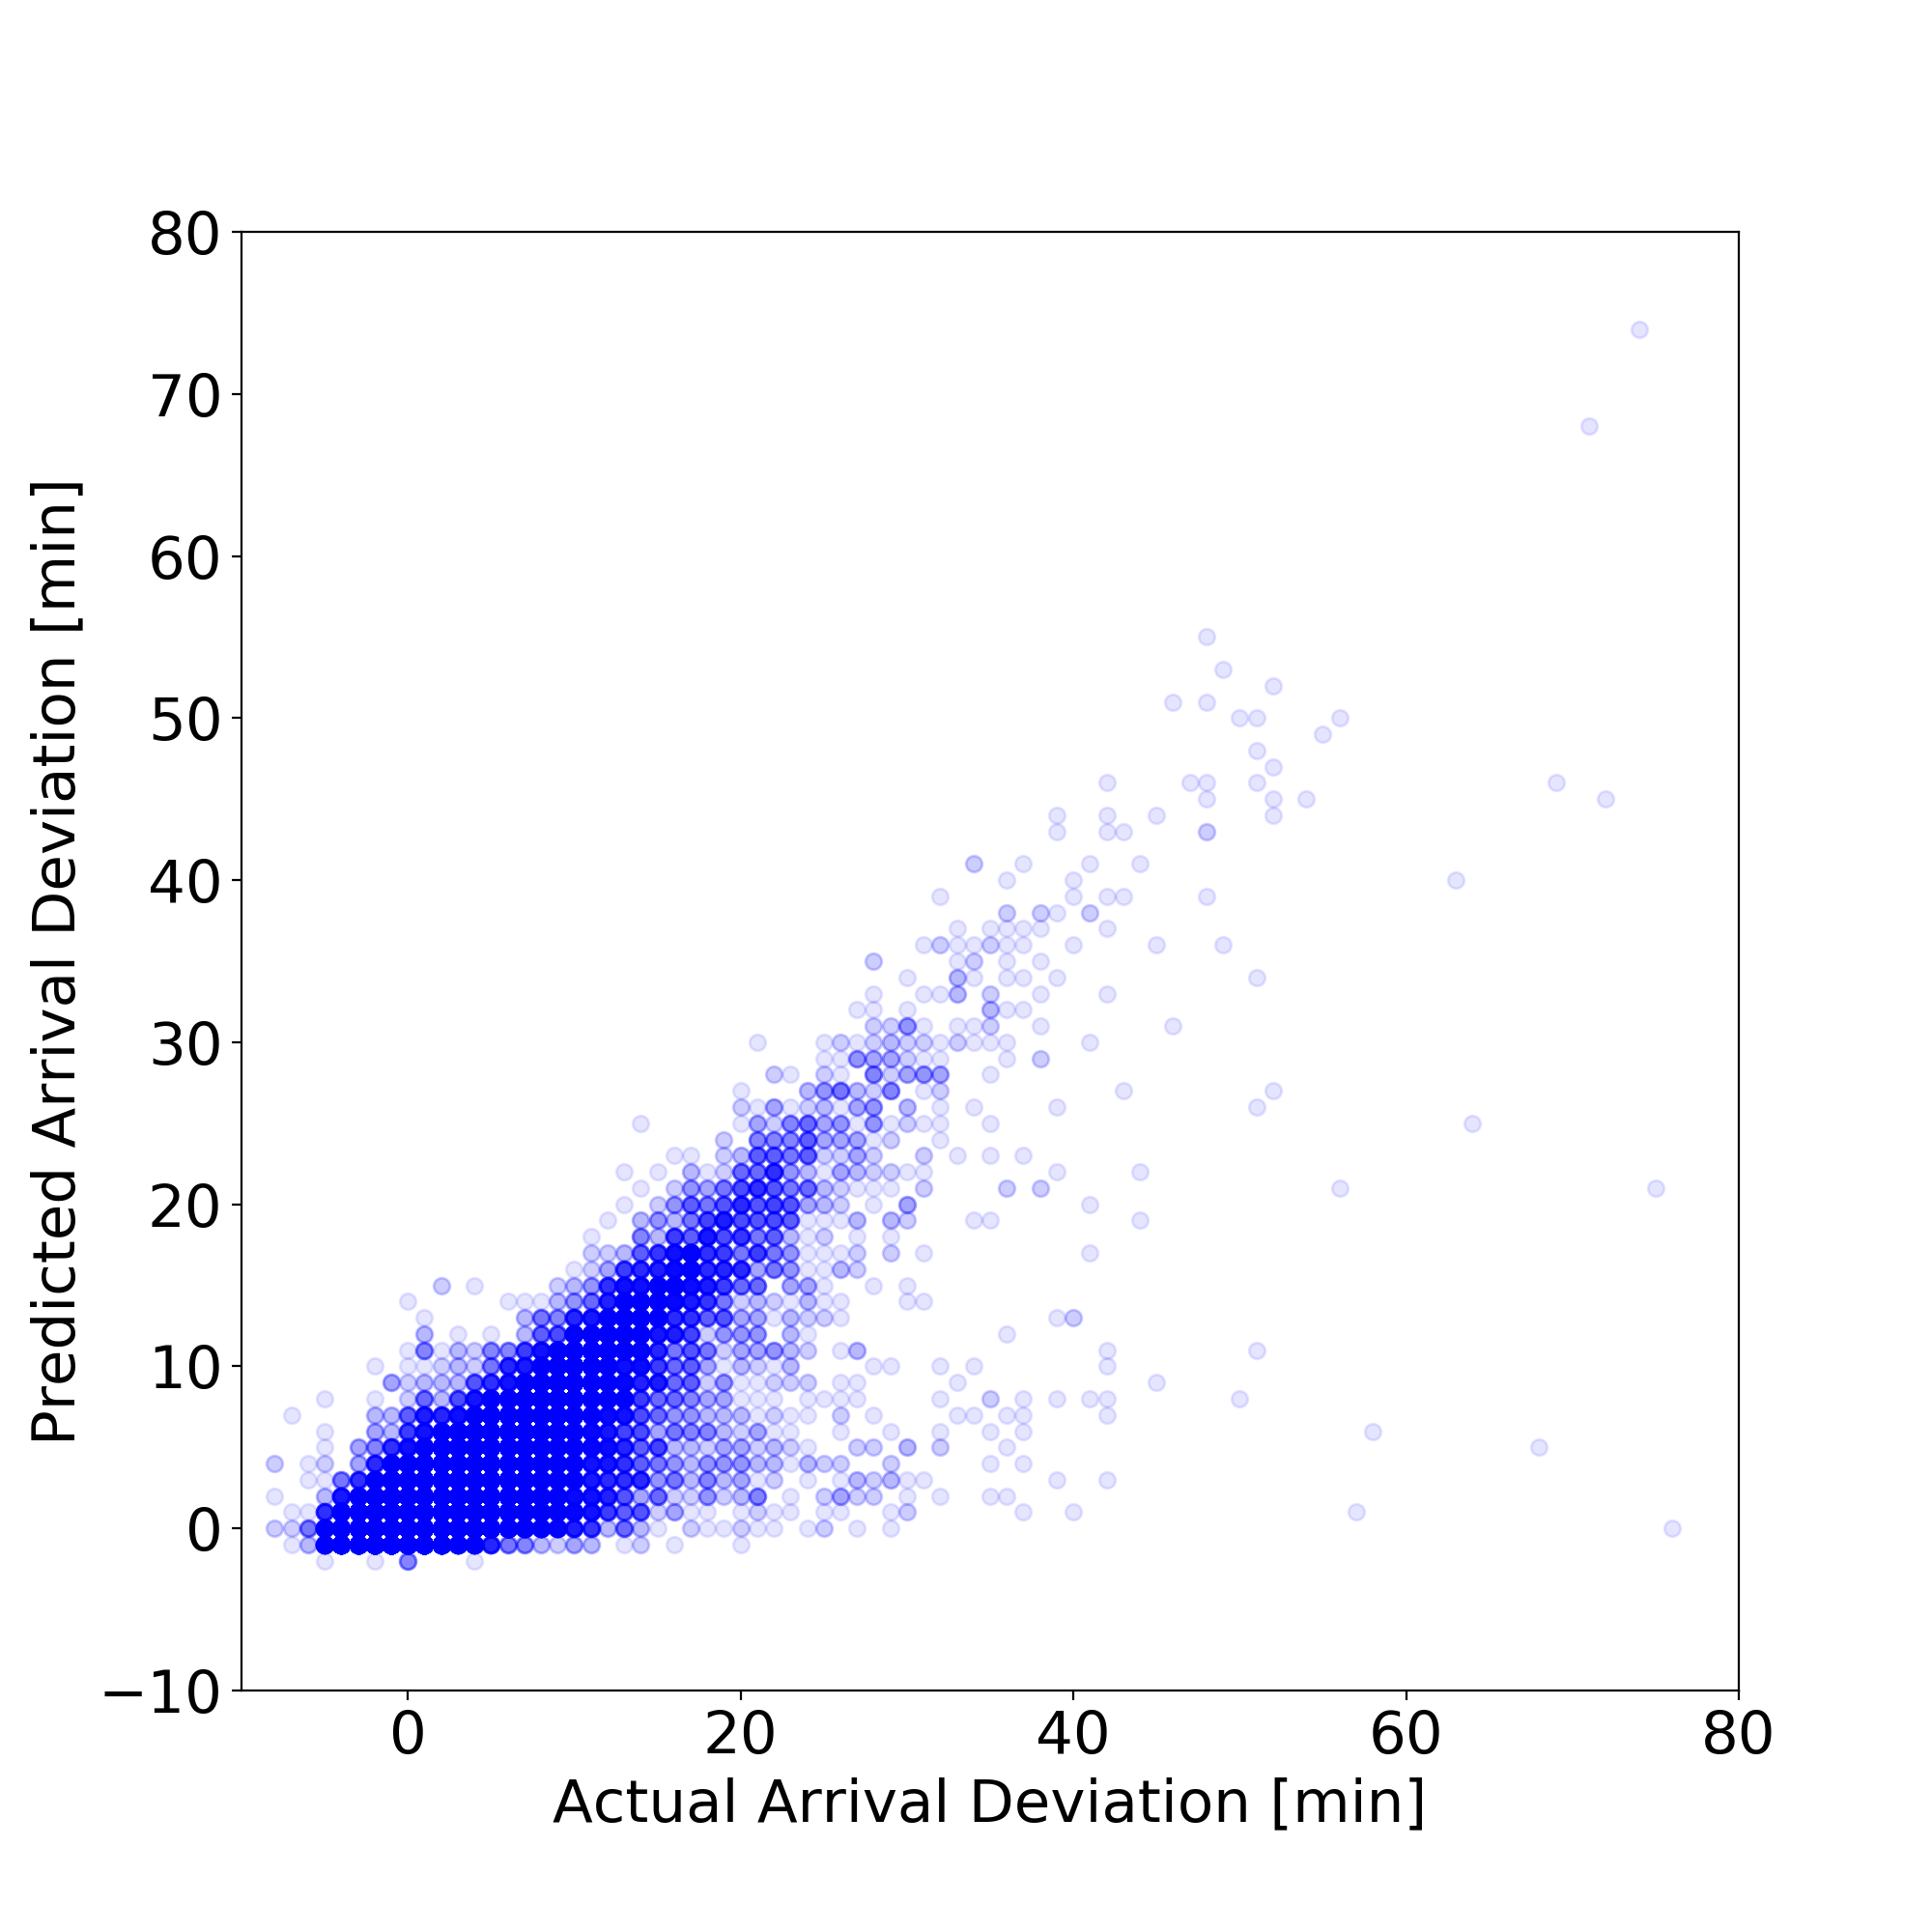
\includegraphics[width=0.5\textwidth]{Images/DNN_plot/2_step/2_step_arrival_deviation.png}\label{fig:2_step_arrival_deviation}}
\subfloat[\tiny{2-Step XGBoost Deviation from Arrival}]{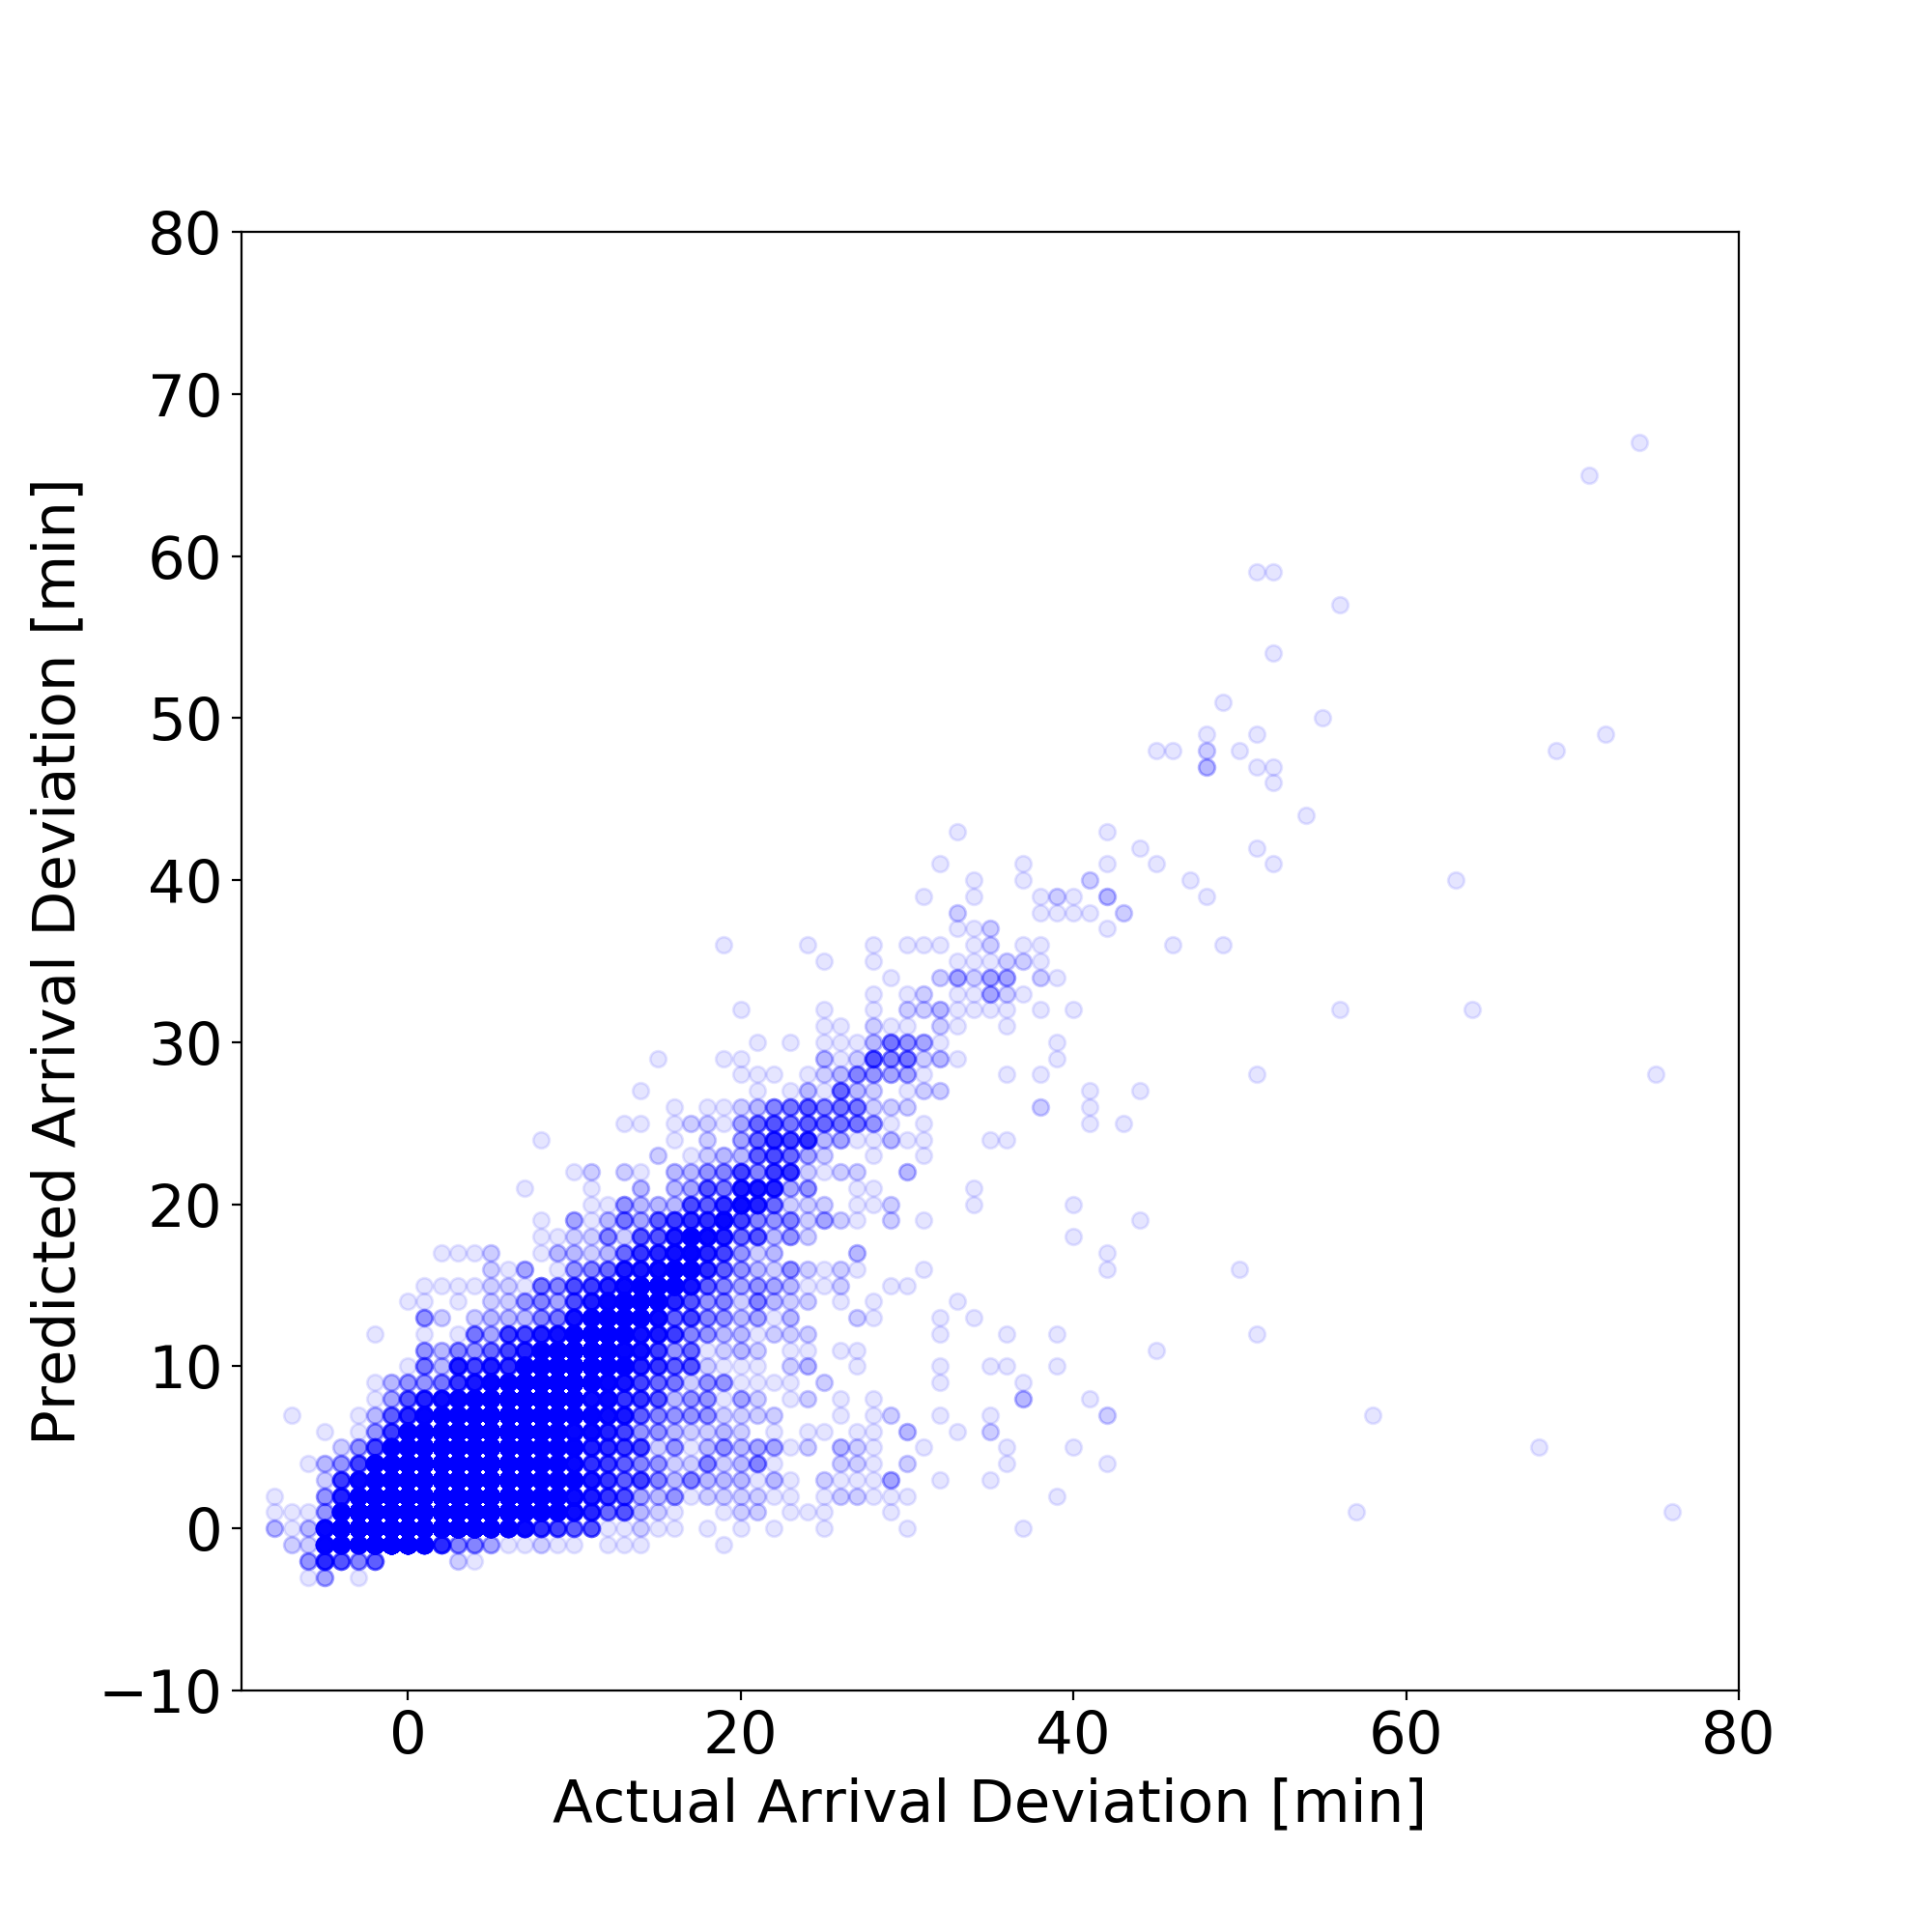
\includegraphics[width=0.5\textwidth]{Images/XGBoost_plot/2_step/2_step_arrival_deviation.png}\label{fig:2_step_arrival_deviation}}
\end{figure}
\begin{figure}[H]
\centering
\subfloat[\tiny{2-Step DNN Deviation from Departure}]{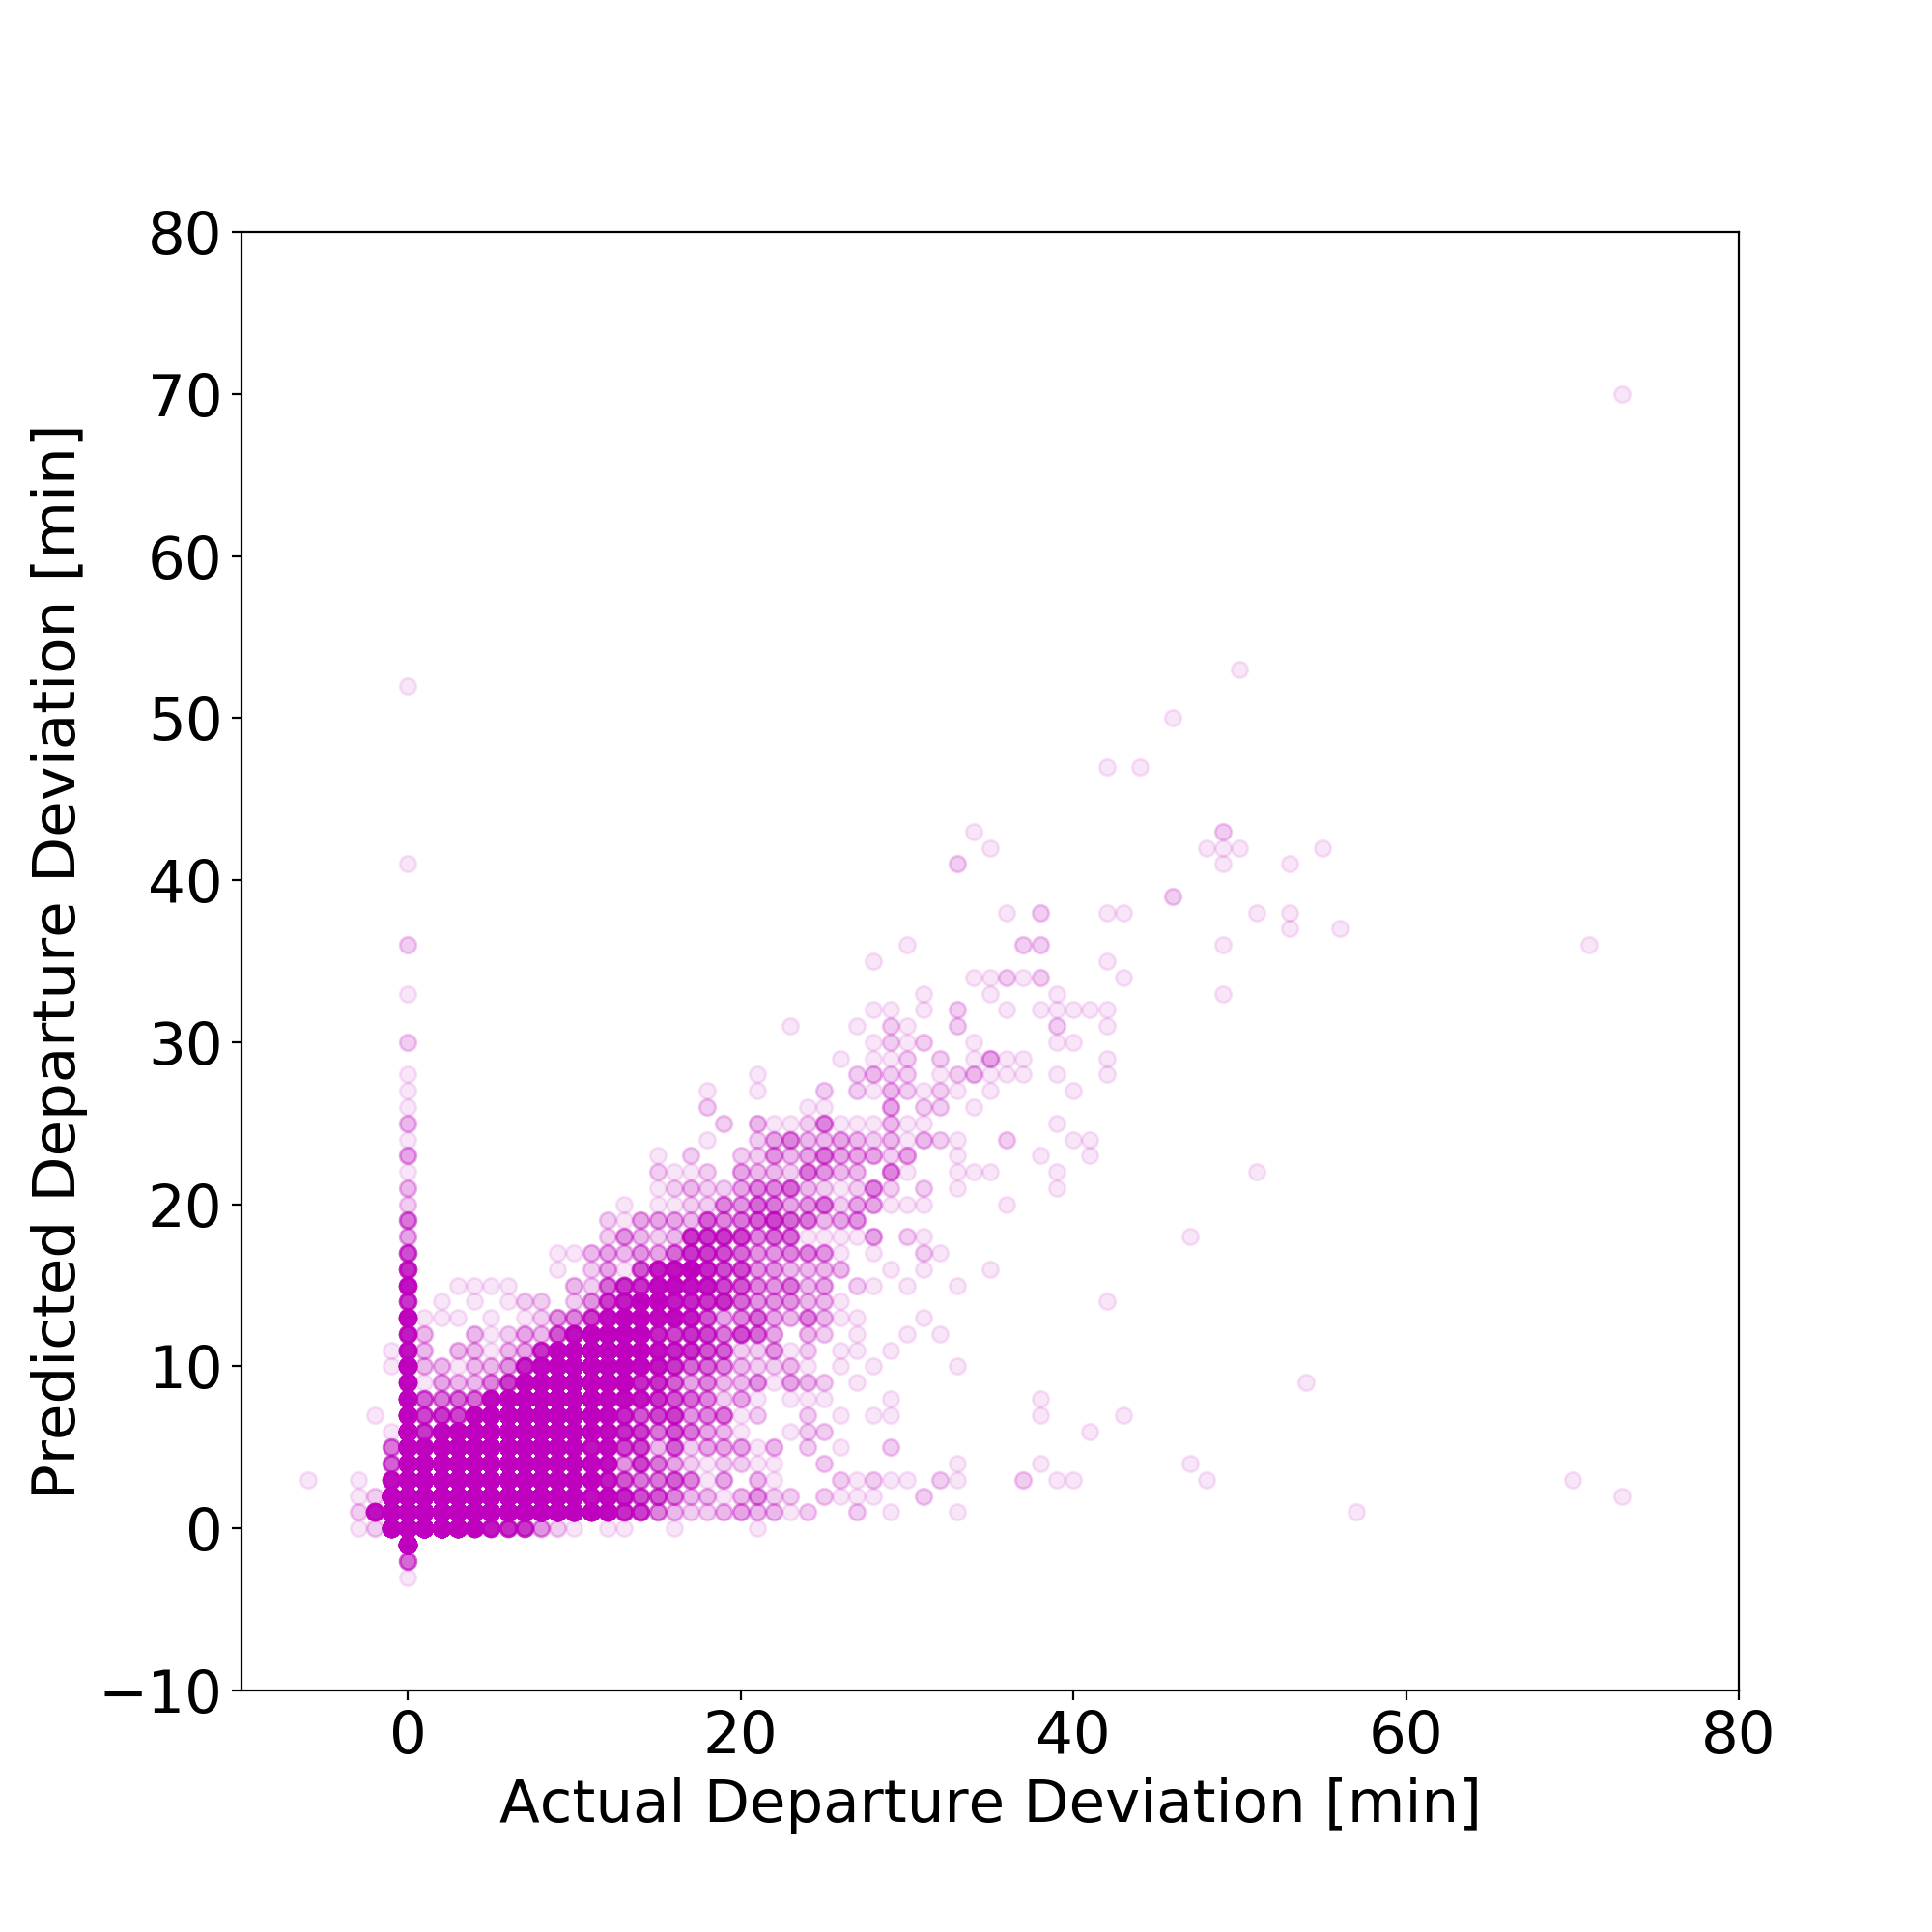
\includegraphics[width=0.5\textwidth]{Images/DNN_plot/2_step/2_step_depature_deviation.png}\label{fig:2_step_depature_deviation}}
\subfloat[\tiny{2-Step XGBoost Deviation from Departure}]{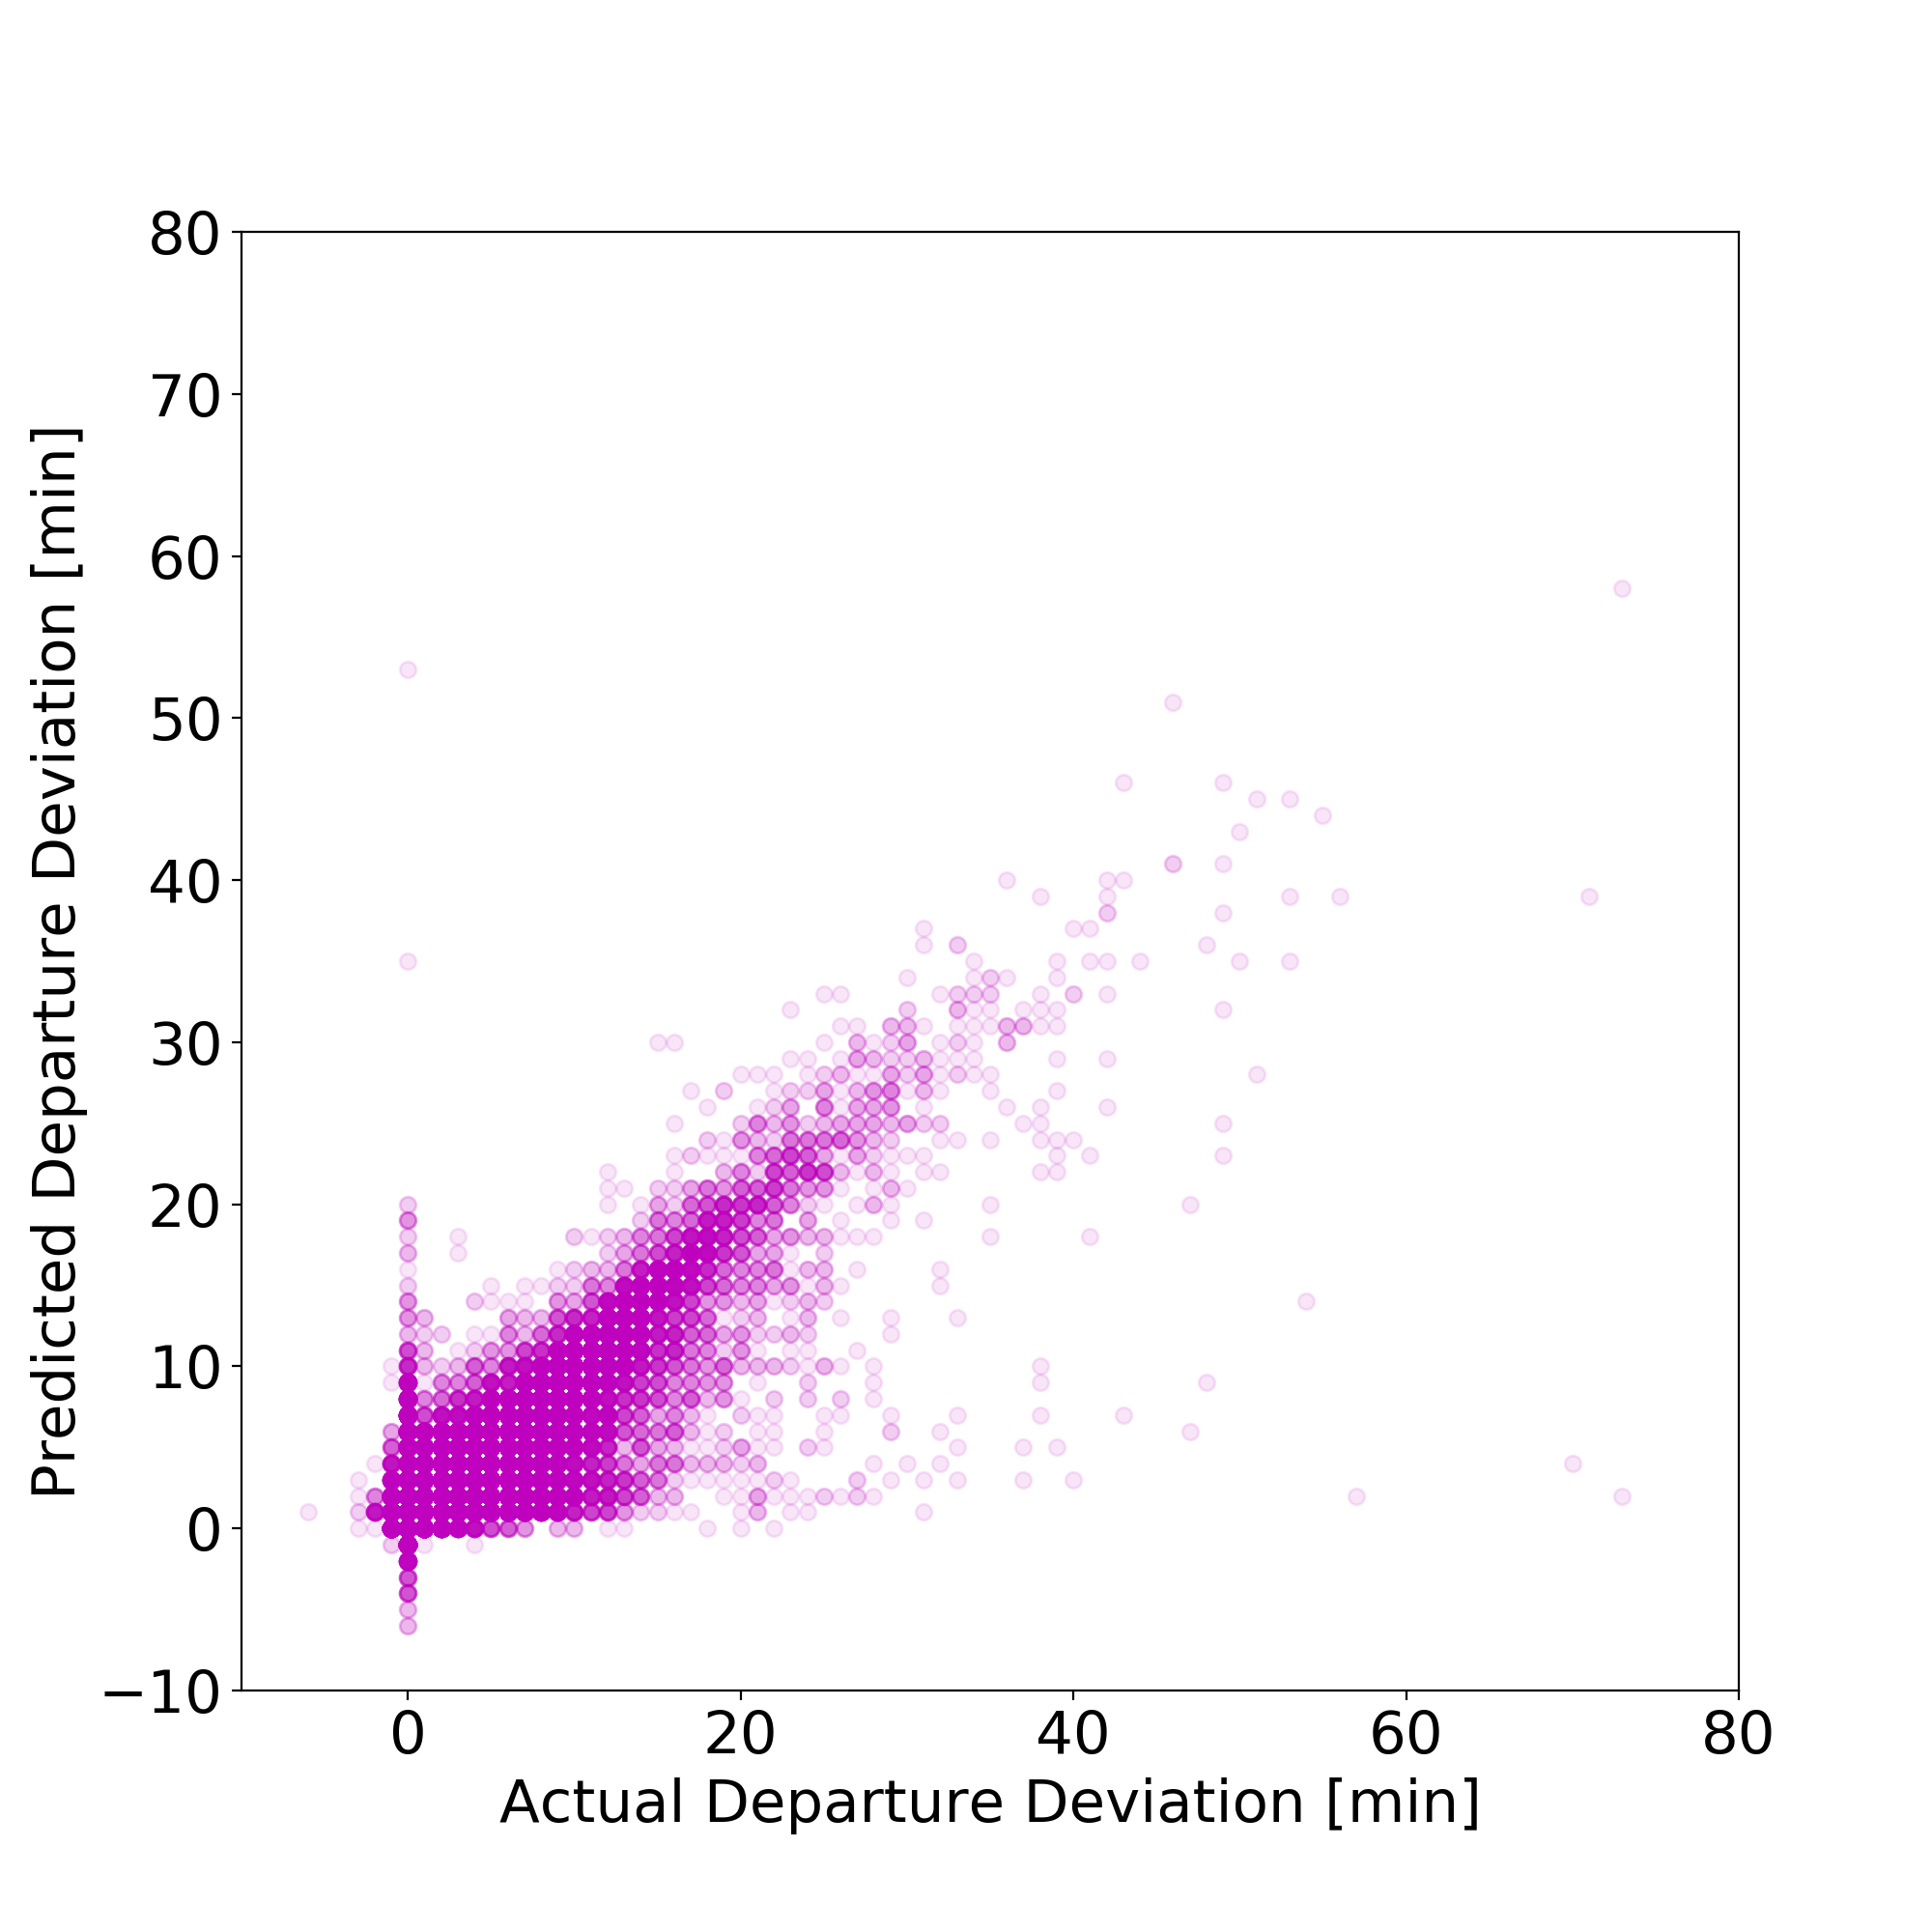
\includegraphics[width=0.5\textwidth]{Images/XGBoost_plot/2_step/2_step_depature_deviation.png}\label{fig:2_step_depature_deviation}}
\end{figure}
\begin{figure}[H]
\centering
\subfloat[\tiny{2-Step DNN Travel Time}]{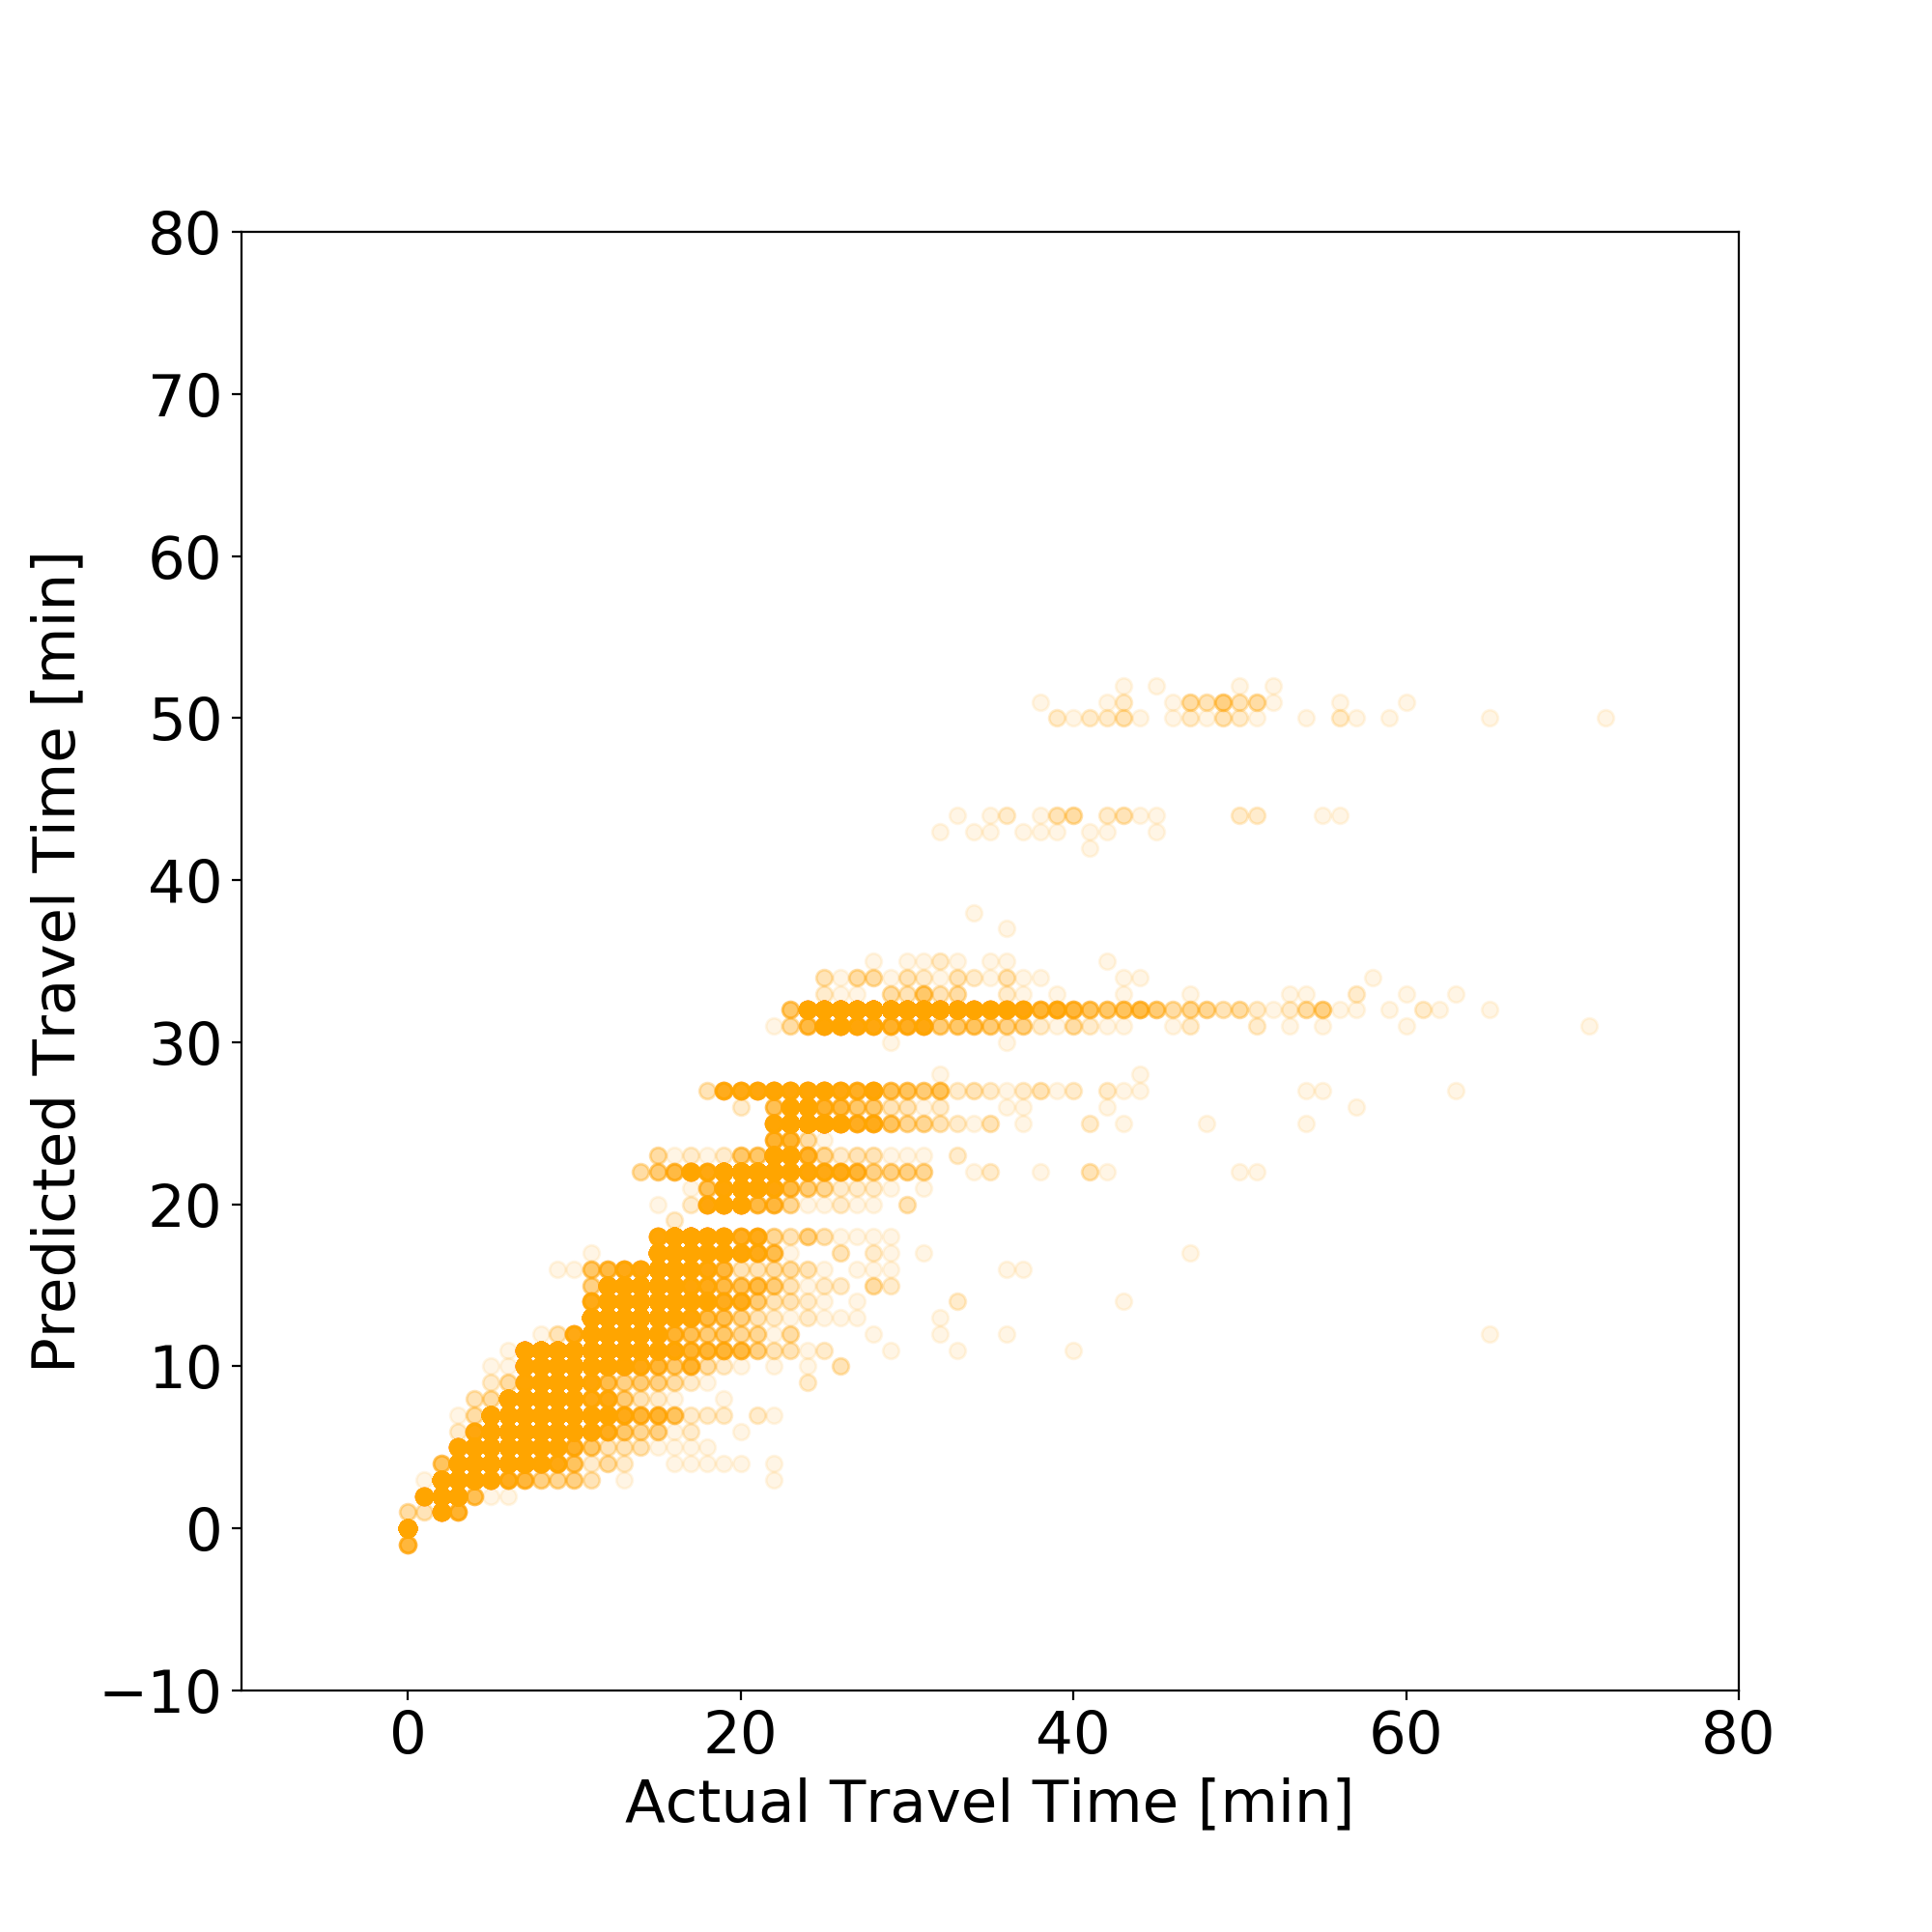
\includegraphics[width=0.5\textwidth]{Images/DNN_plot/2_step/2_step_travel_time.png}\label{fig:2_step_travel_time}}
\subfloat[\tiny{2-Step XGBoost Travel Time}]{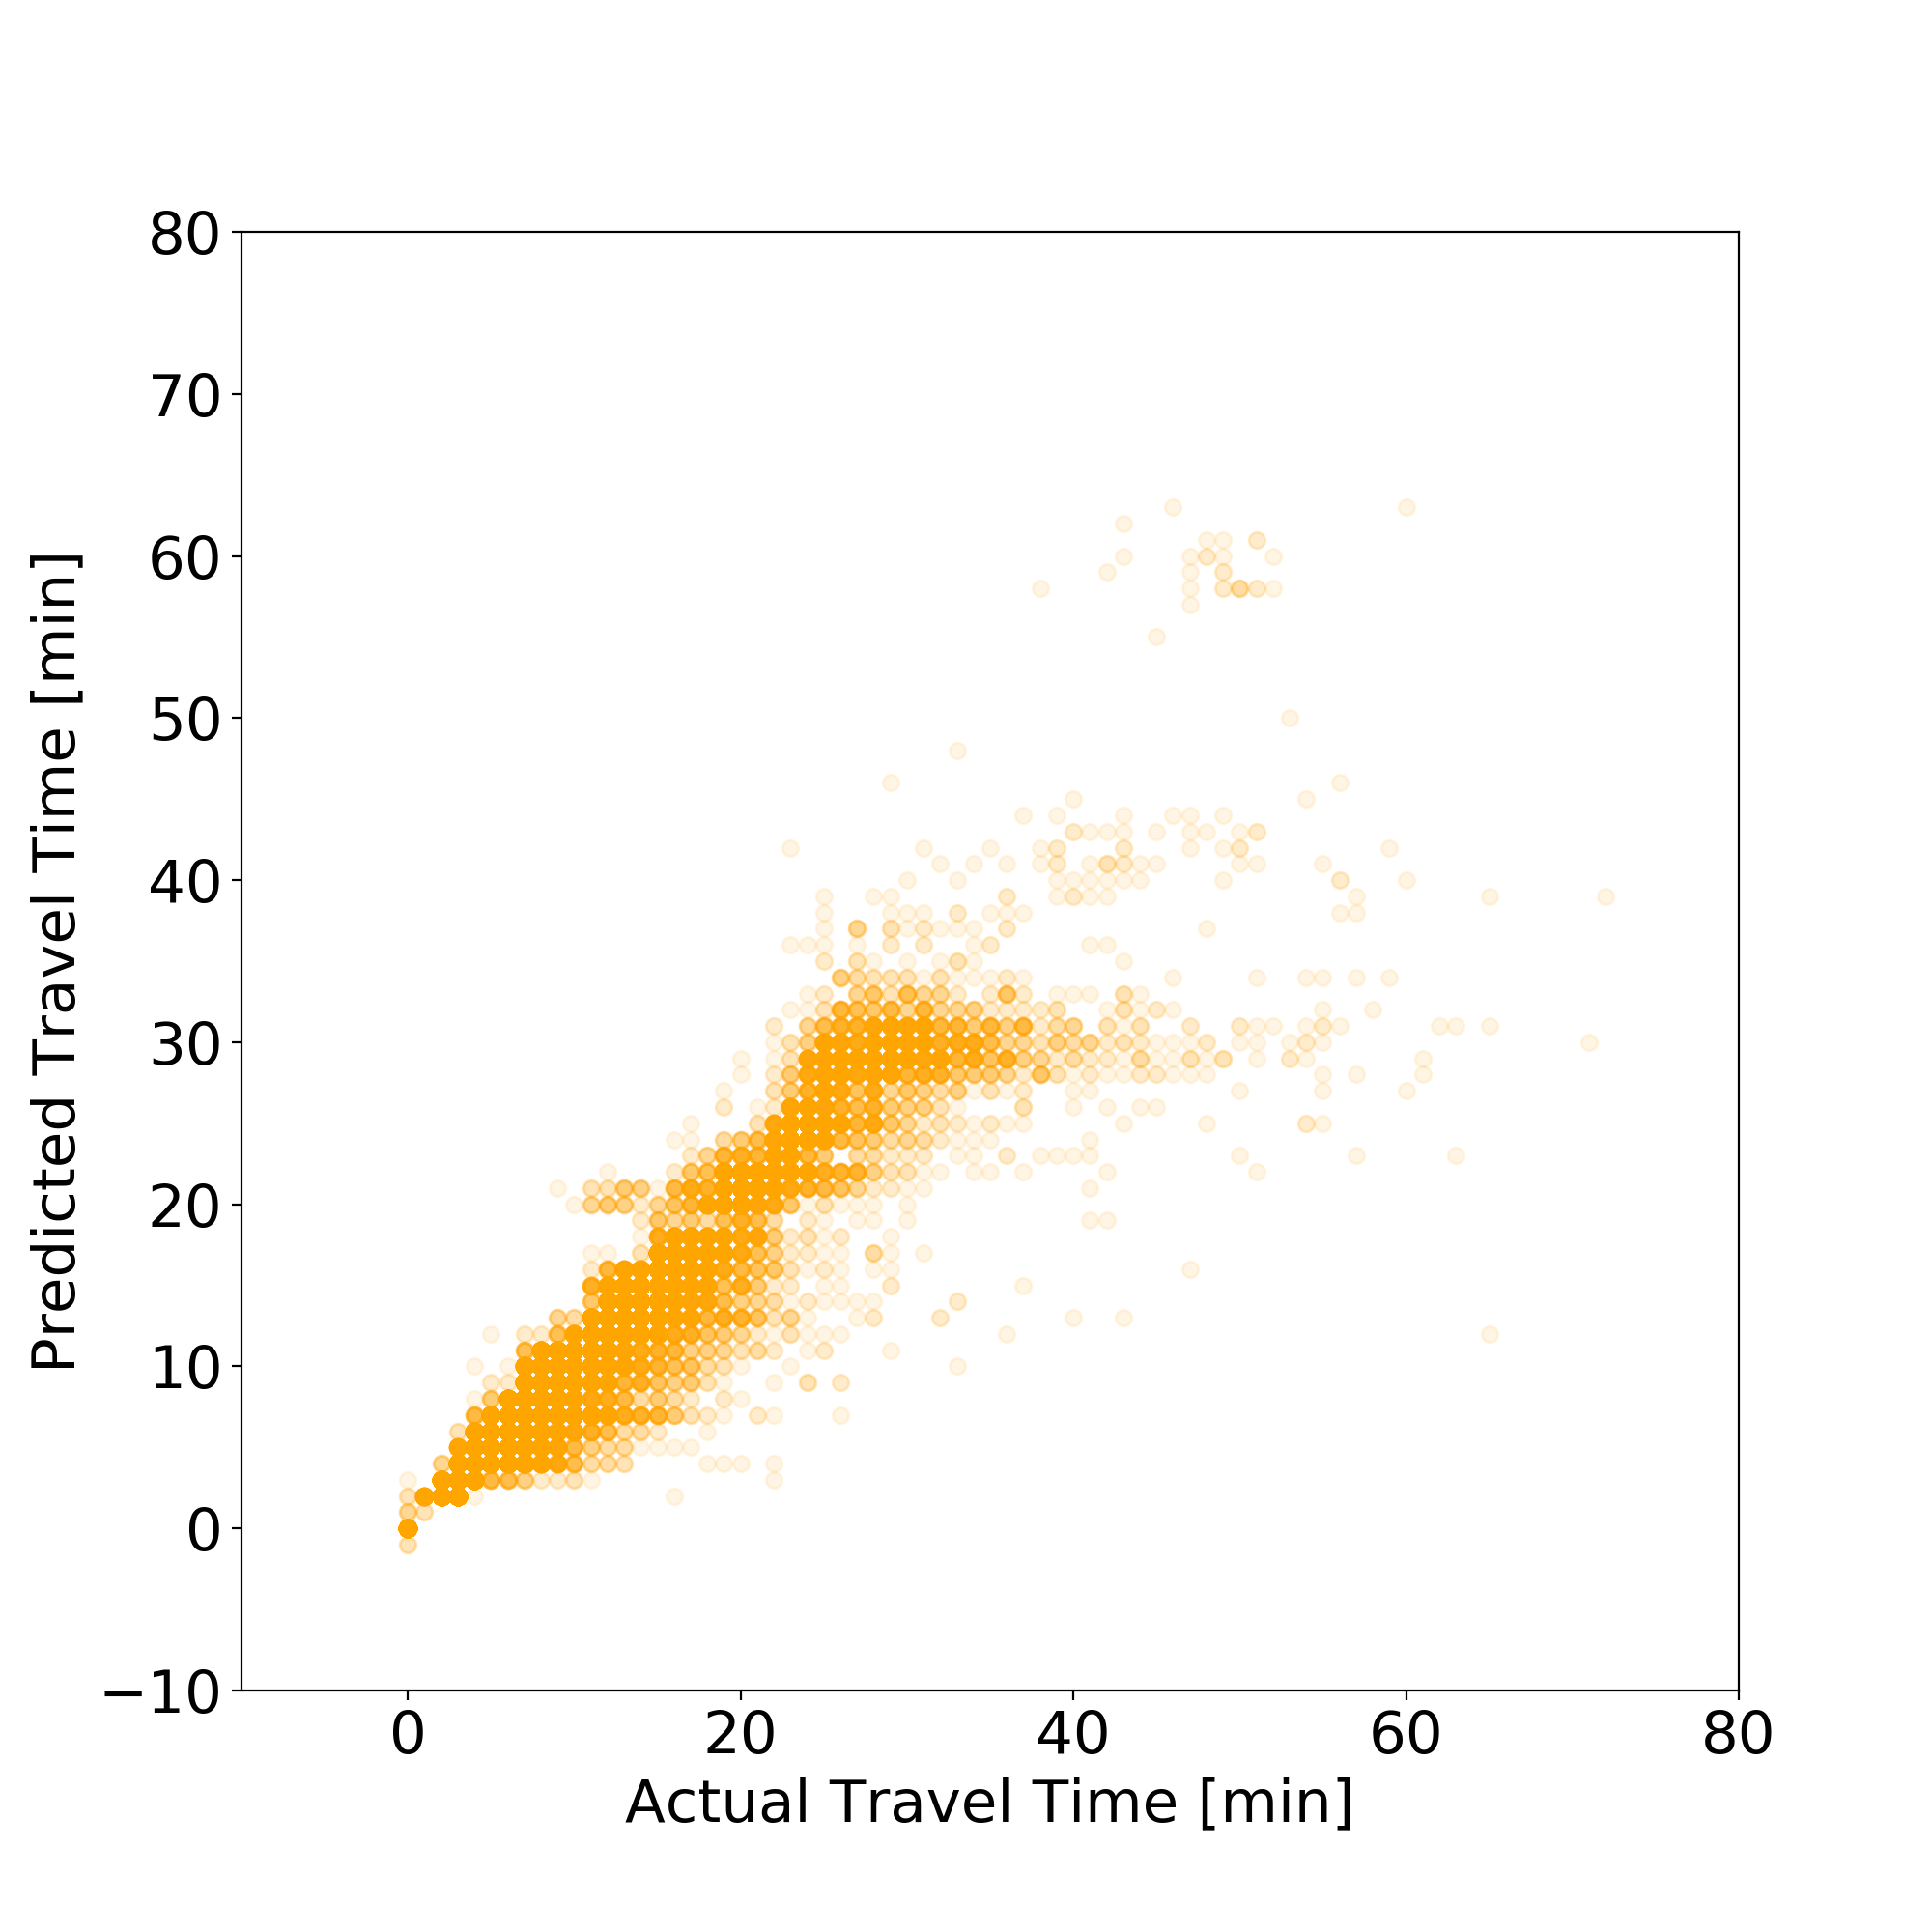
\includegraphics[width=0.5\textwidth]{Images/XGBoost_plot/2_step/2_step_travel_time.png}\label{fig:2_step_travel_time}}
\end{figure}
\begin{figure}[H]
\centering
\subfloat[\tiny{2-Step DNN Dwell Time}]{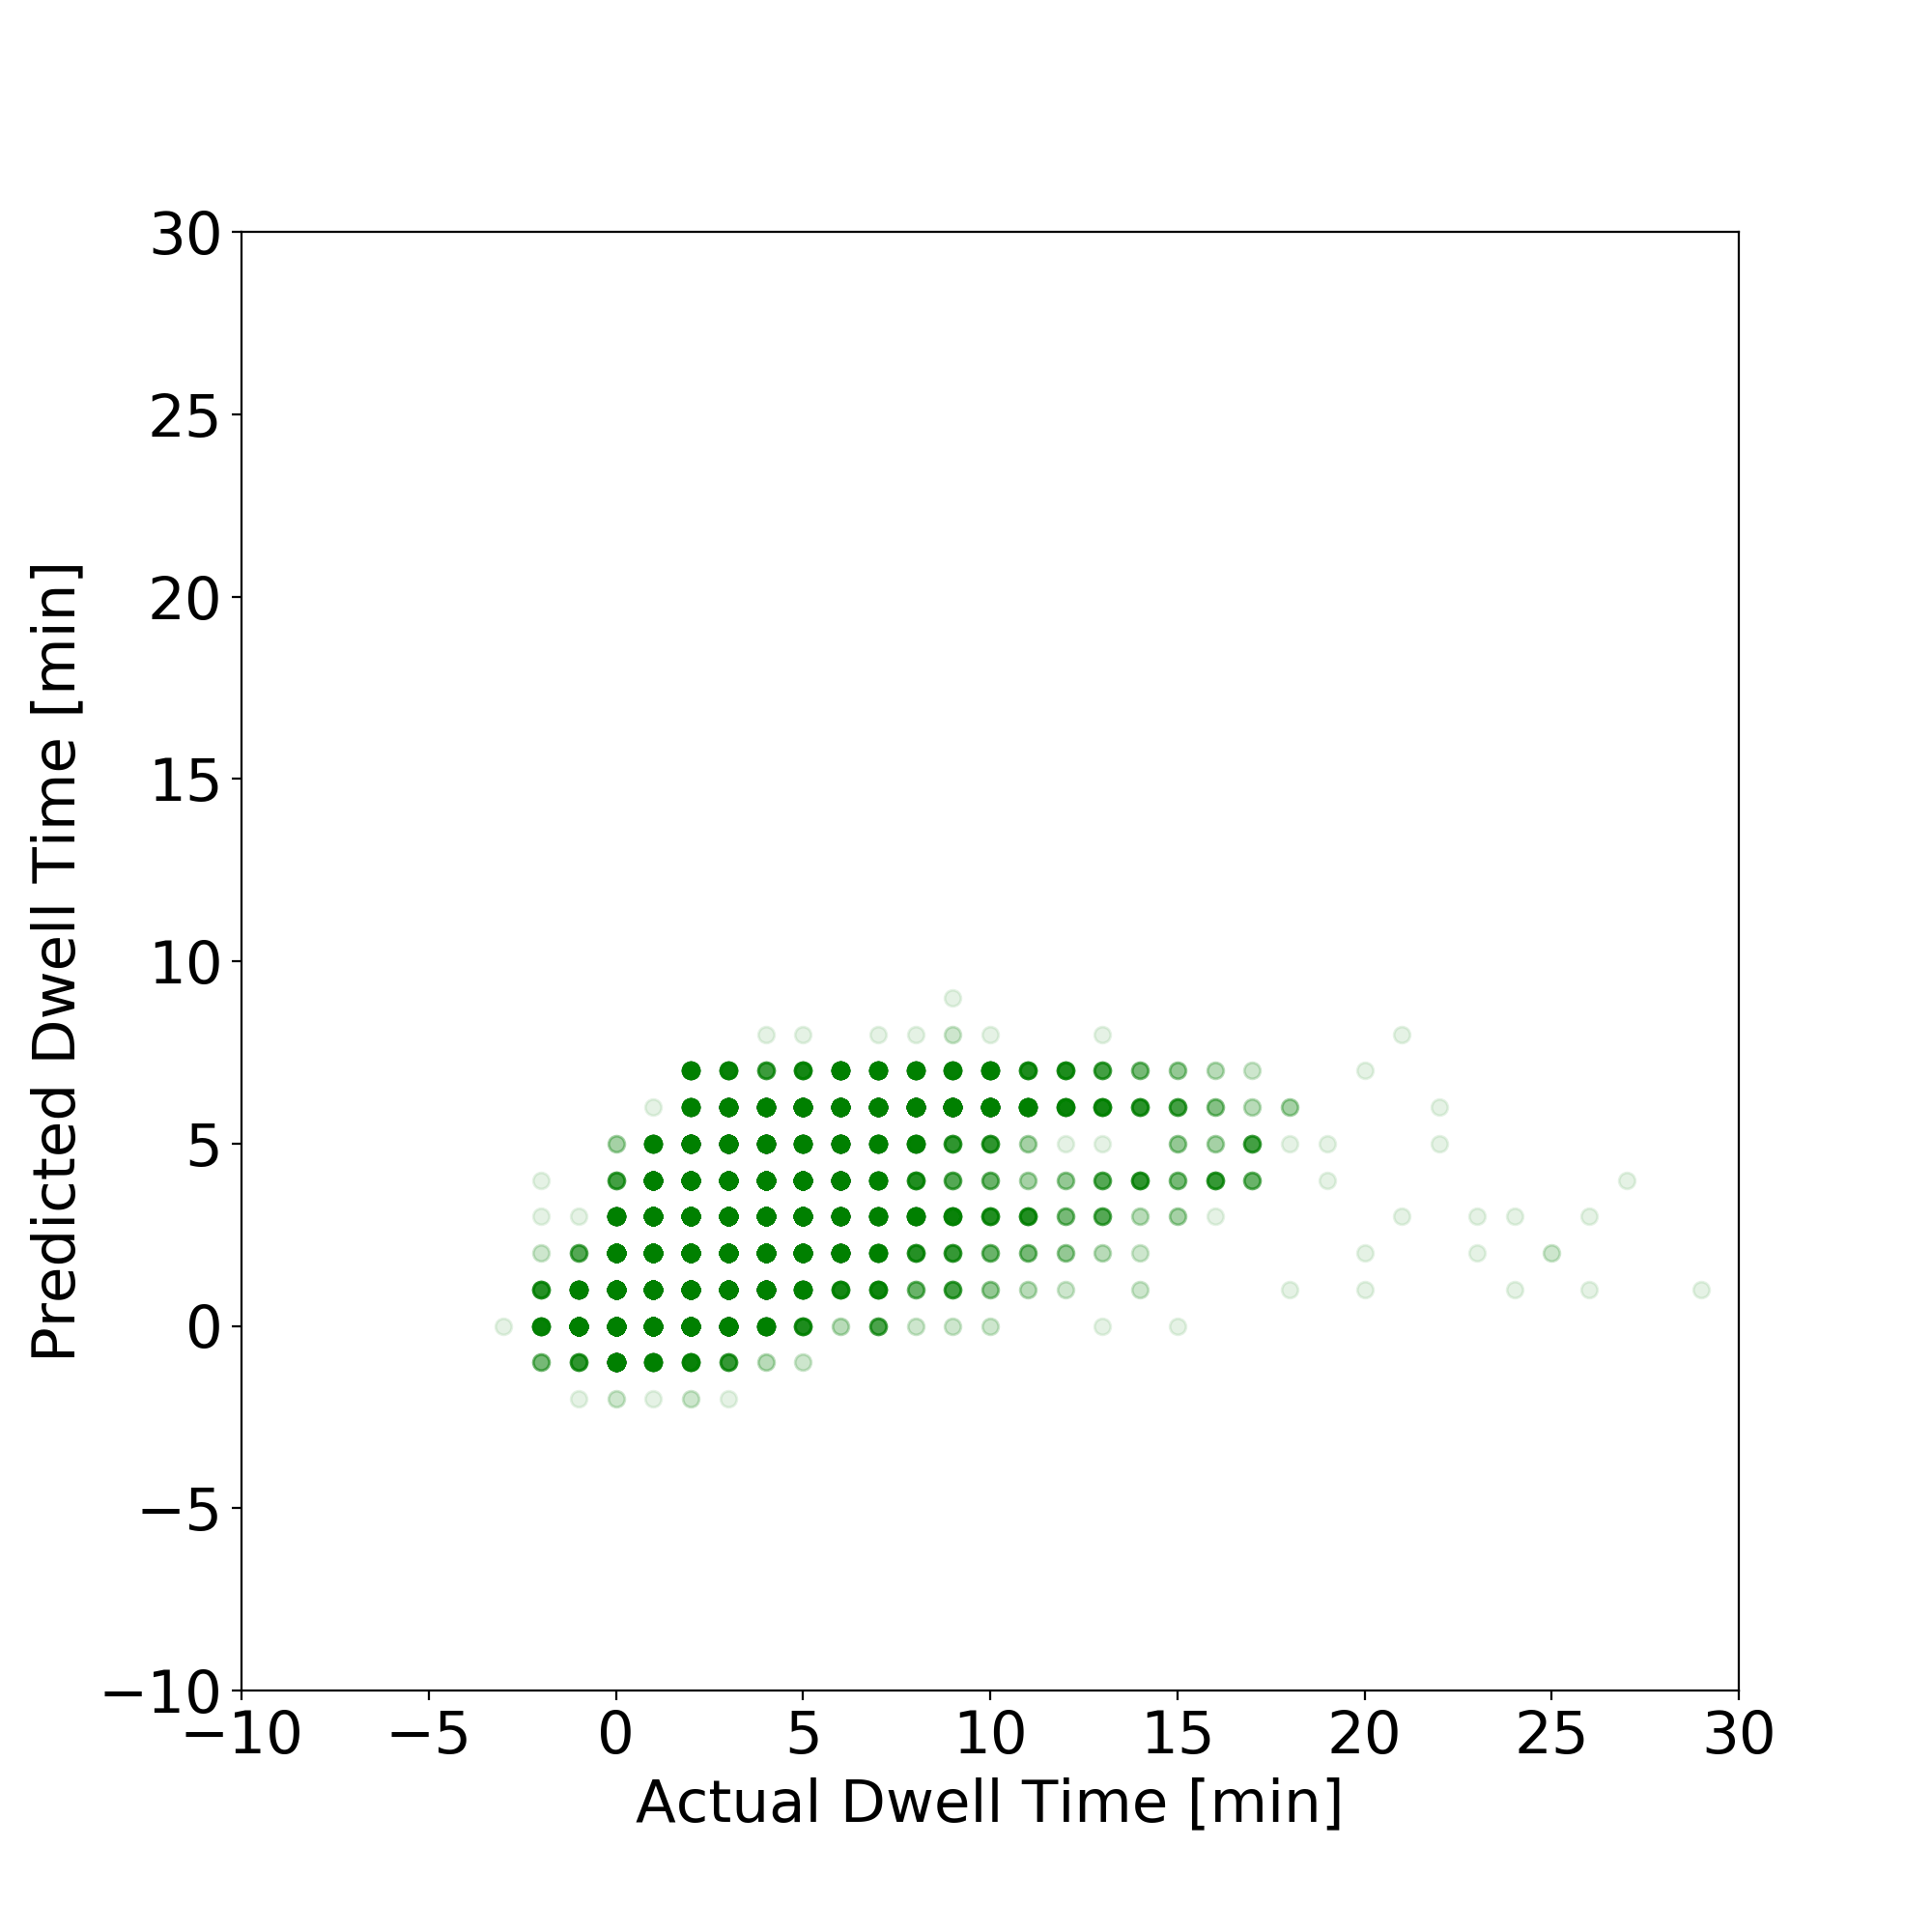
\includegraphics[width=0.5\textwidth]{Images/DNN_plot/2_step/2_step_dwell_time.png}\label{fig:2_step_dwell_time}}
\subfloat[\tiny{2-Step XGBoost Dwell Time}]{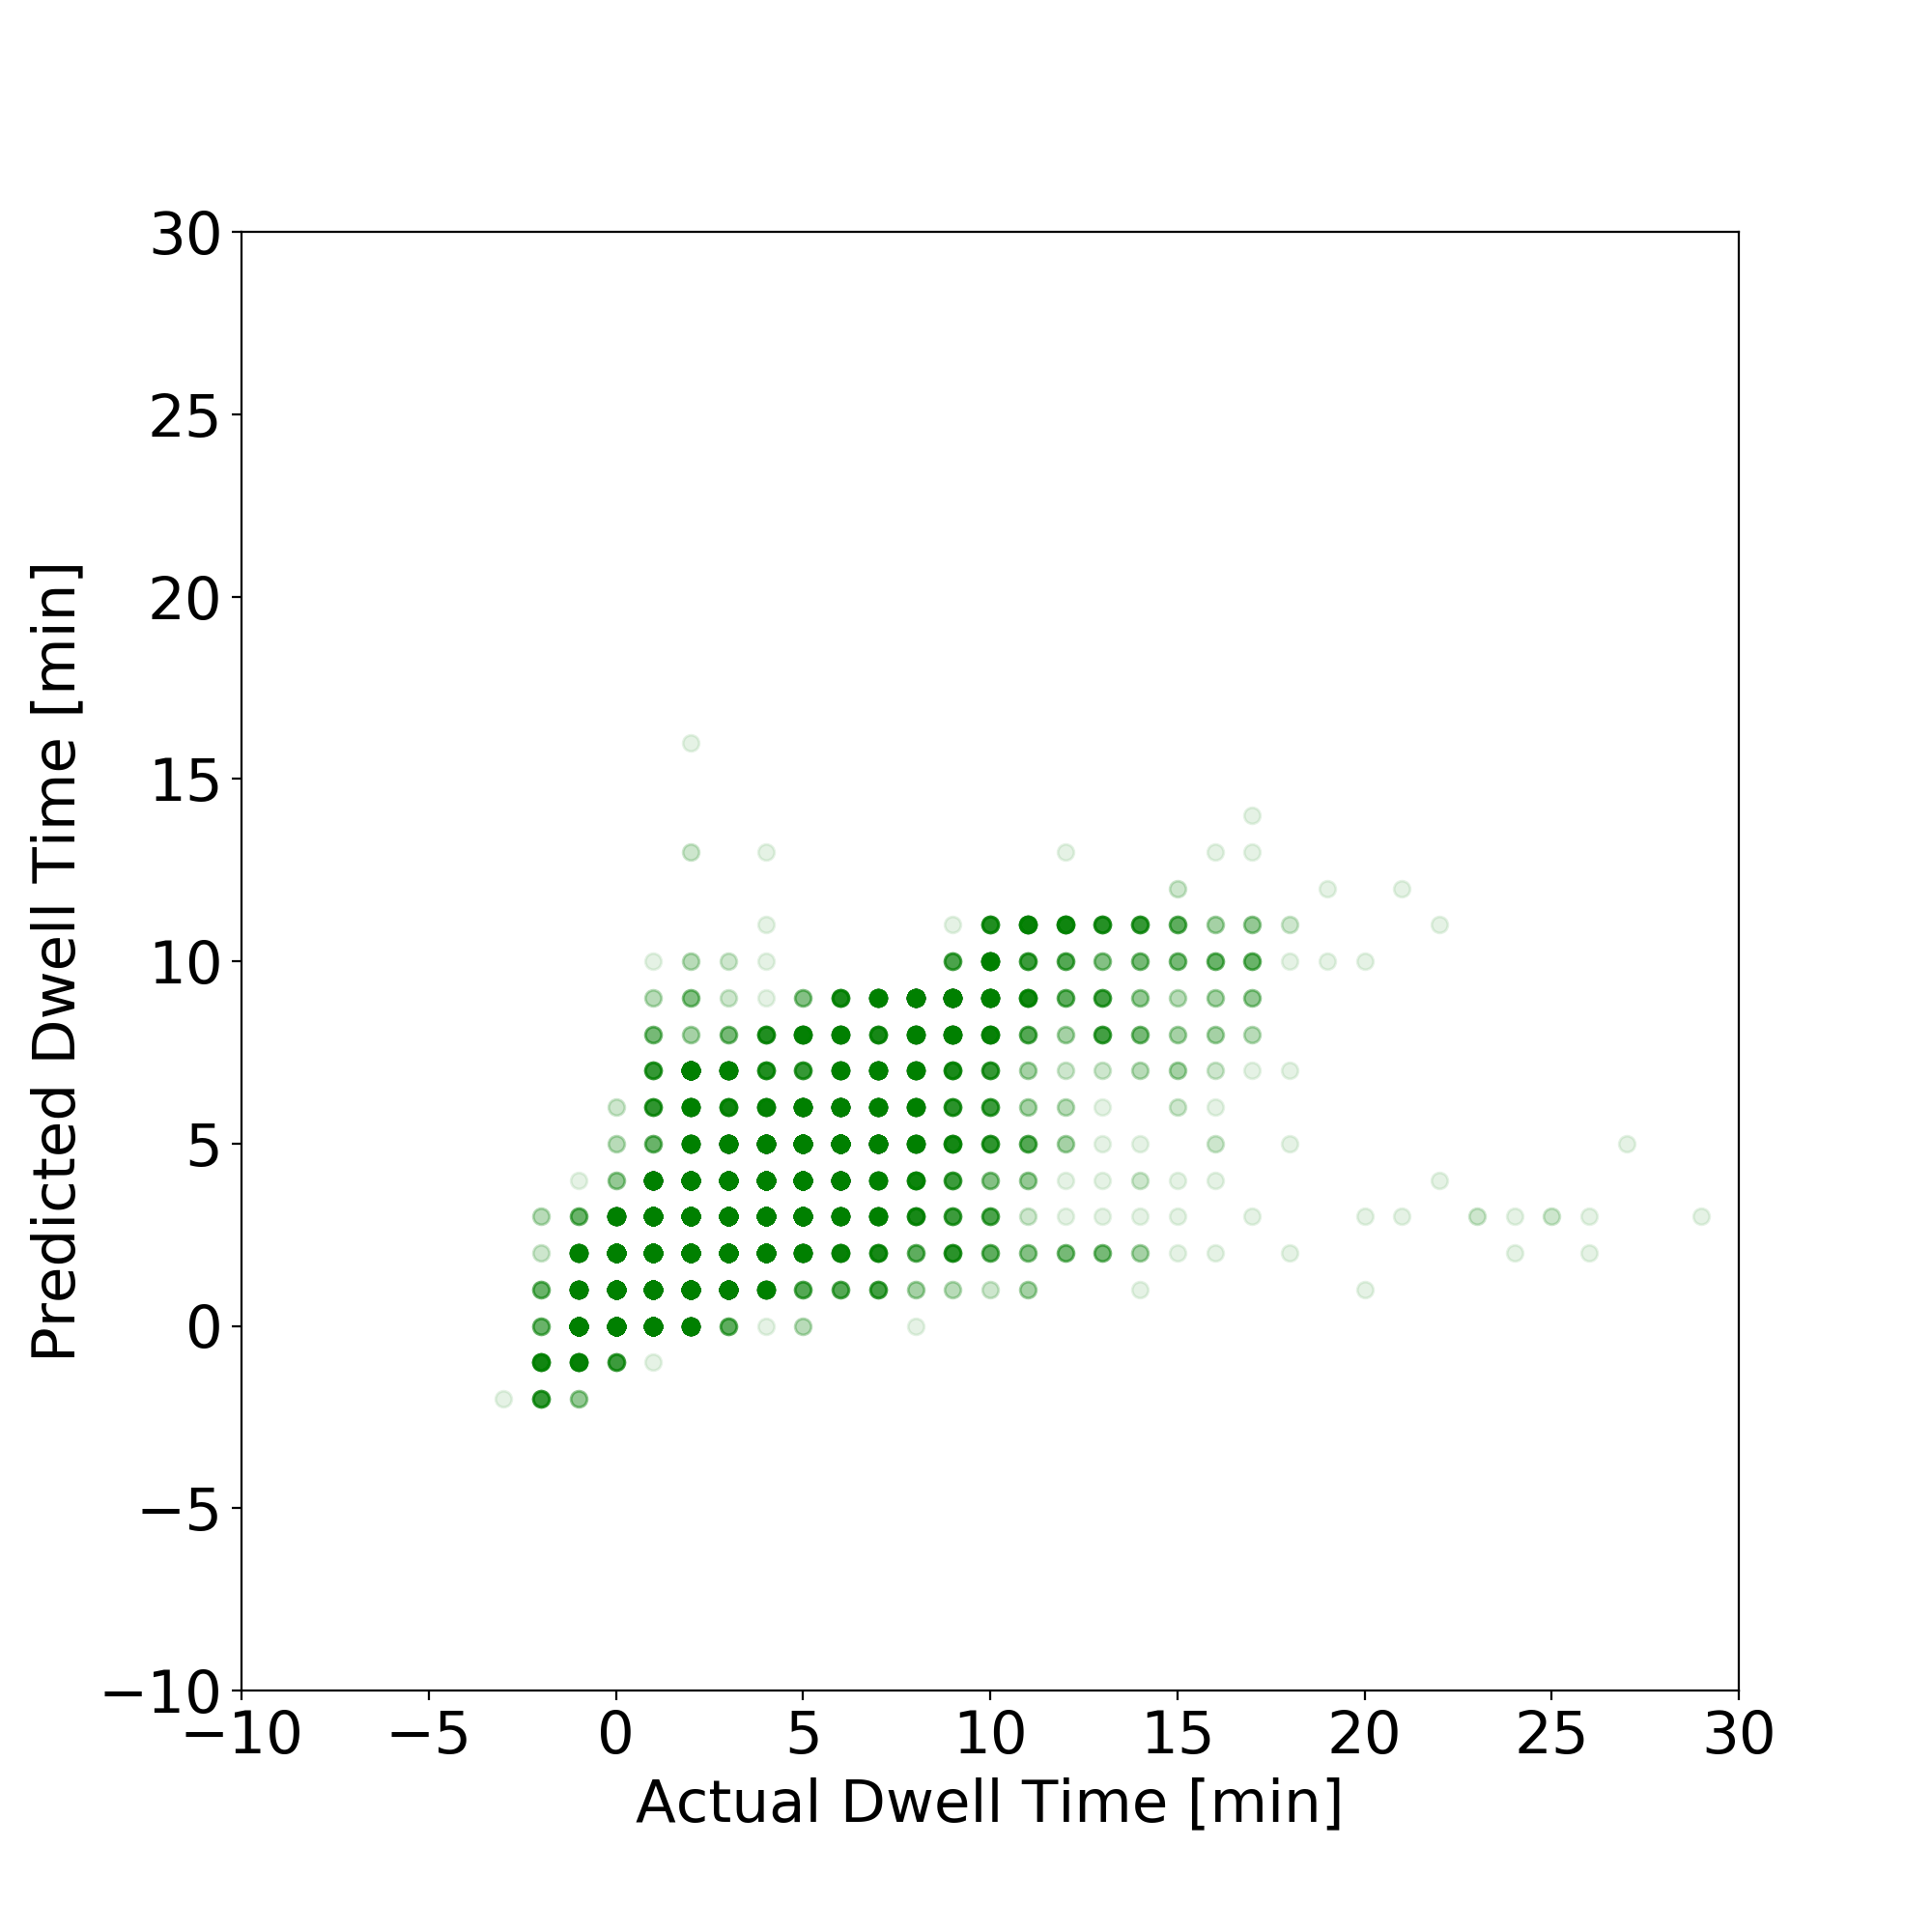
\includegraphics[width=0.5\textwidth]{Images/XGBoost_plot/2_step/2_step_dwell_time.png}\label{fig:2_step_dwell_time}}
\end{figure}

\begin{figure}[H]
\centering
\subfloat[\tiny{3-Step DNN Deviation from Arrival}]{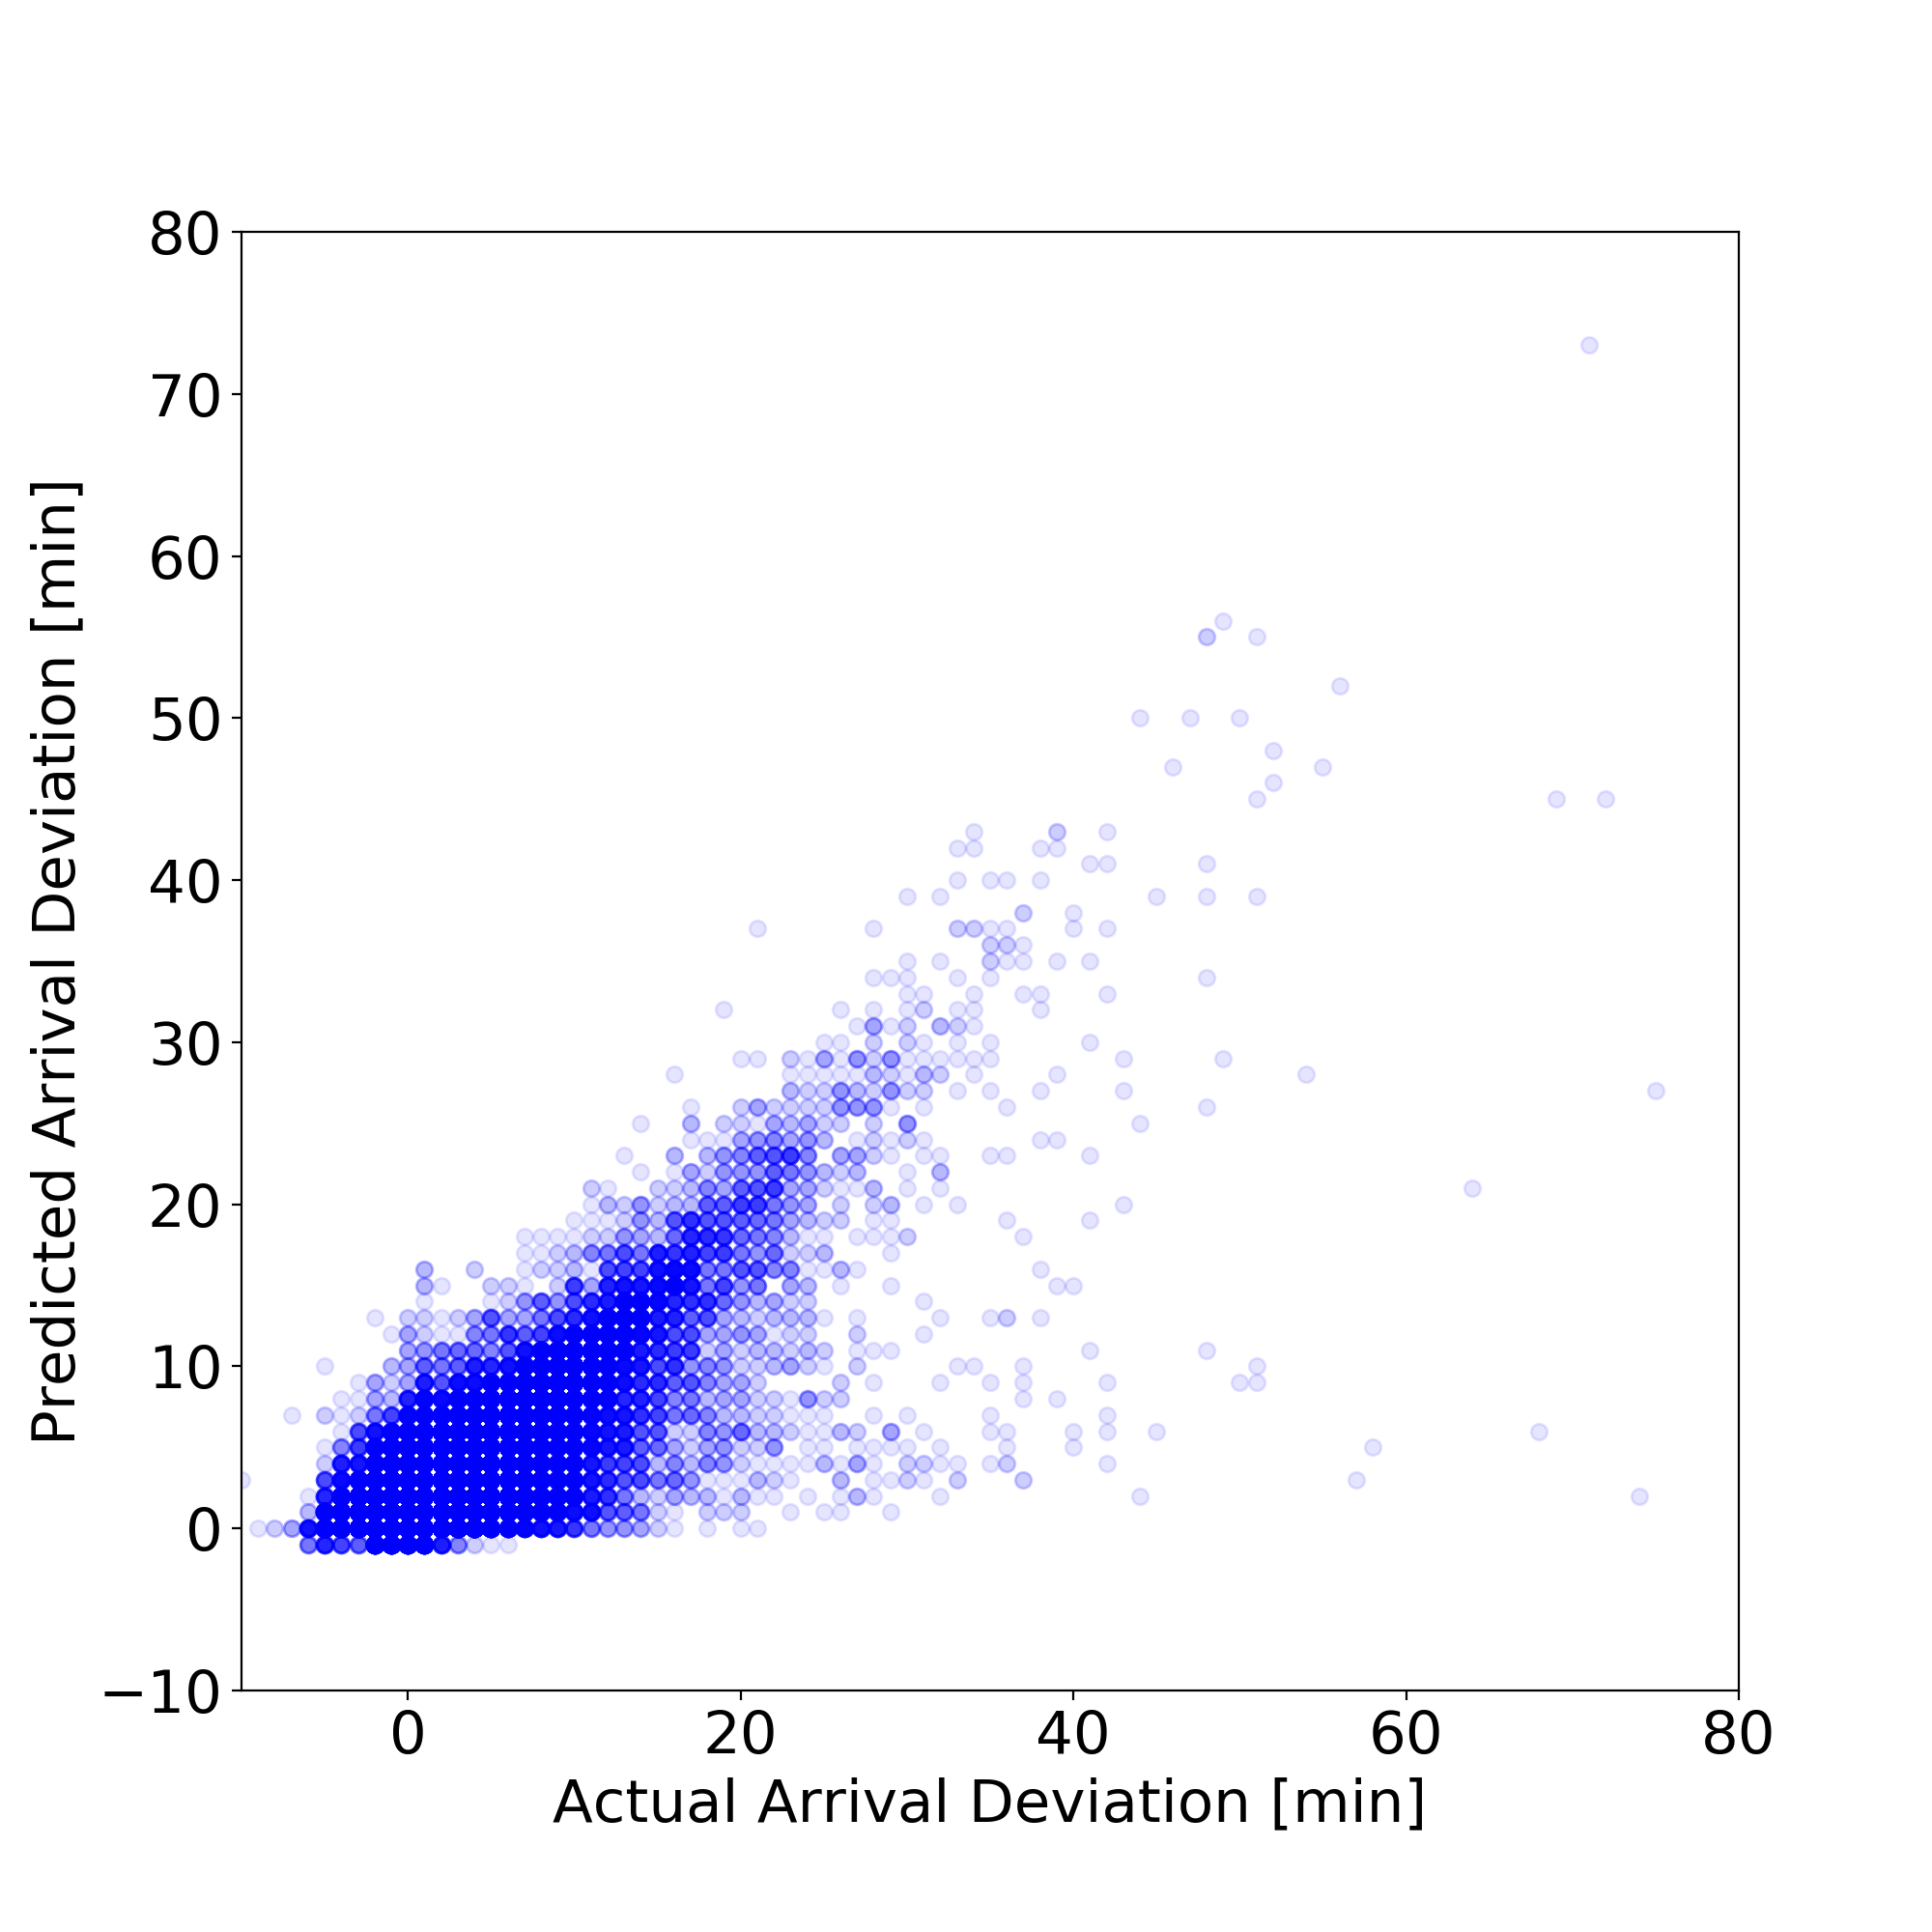
\includegraphics[width=0.5\textwidth]{Images/DNN_plot/3_step/3_step_arrival_deviation.png}\label{fig:3_step_arrival_deviation}}
\subfloat[\tiny{3-Step XGBoost Deviation from Arrival}]{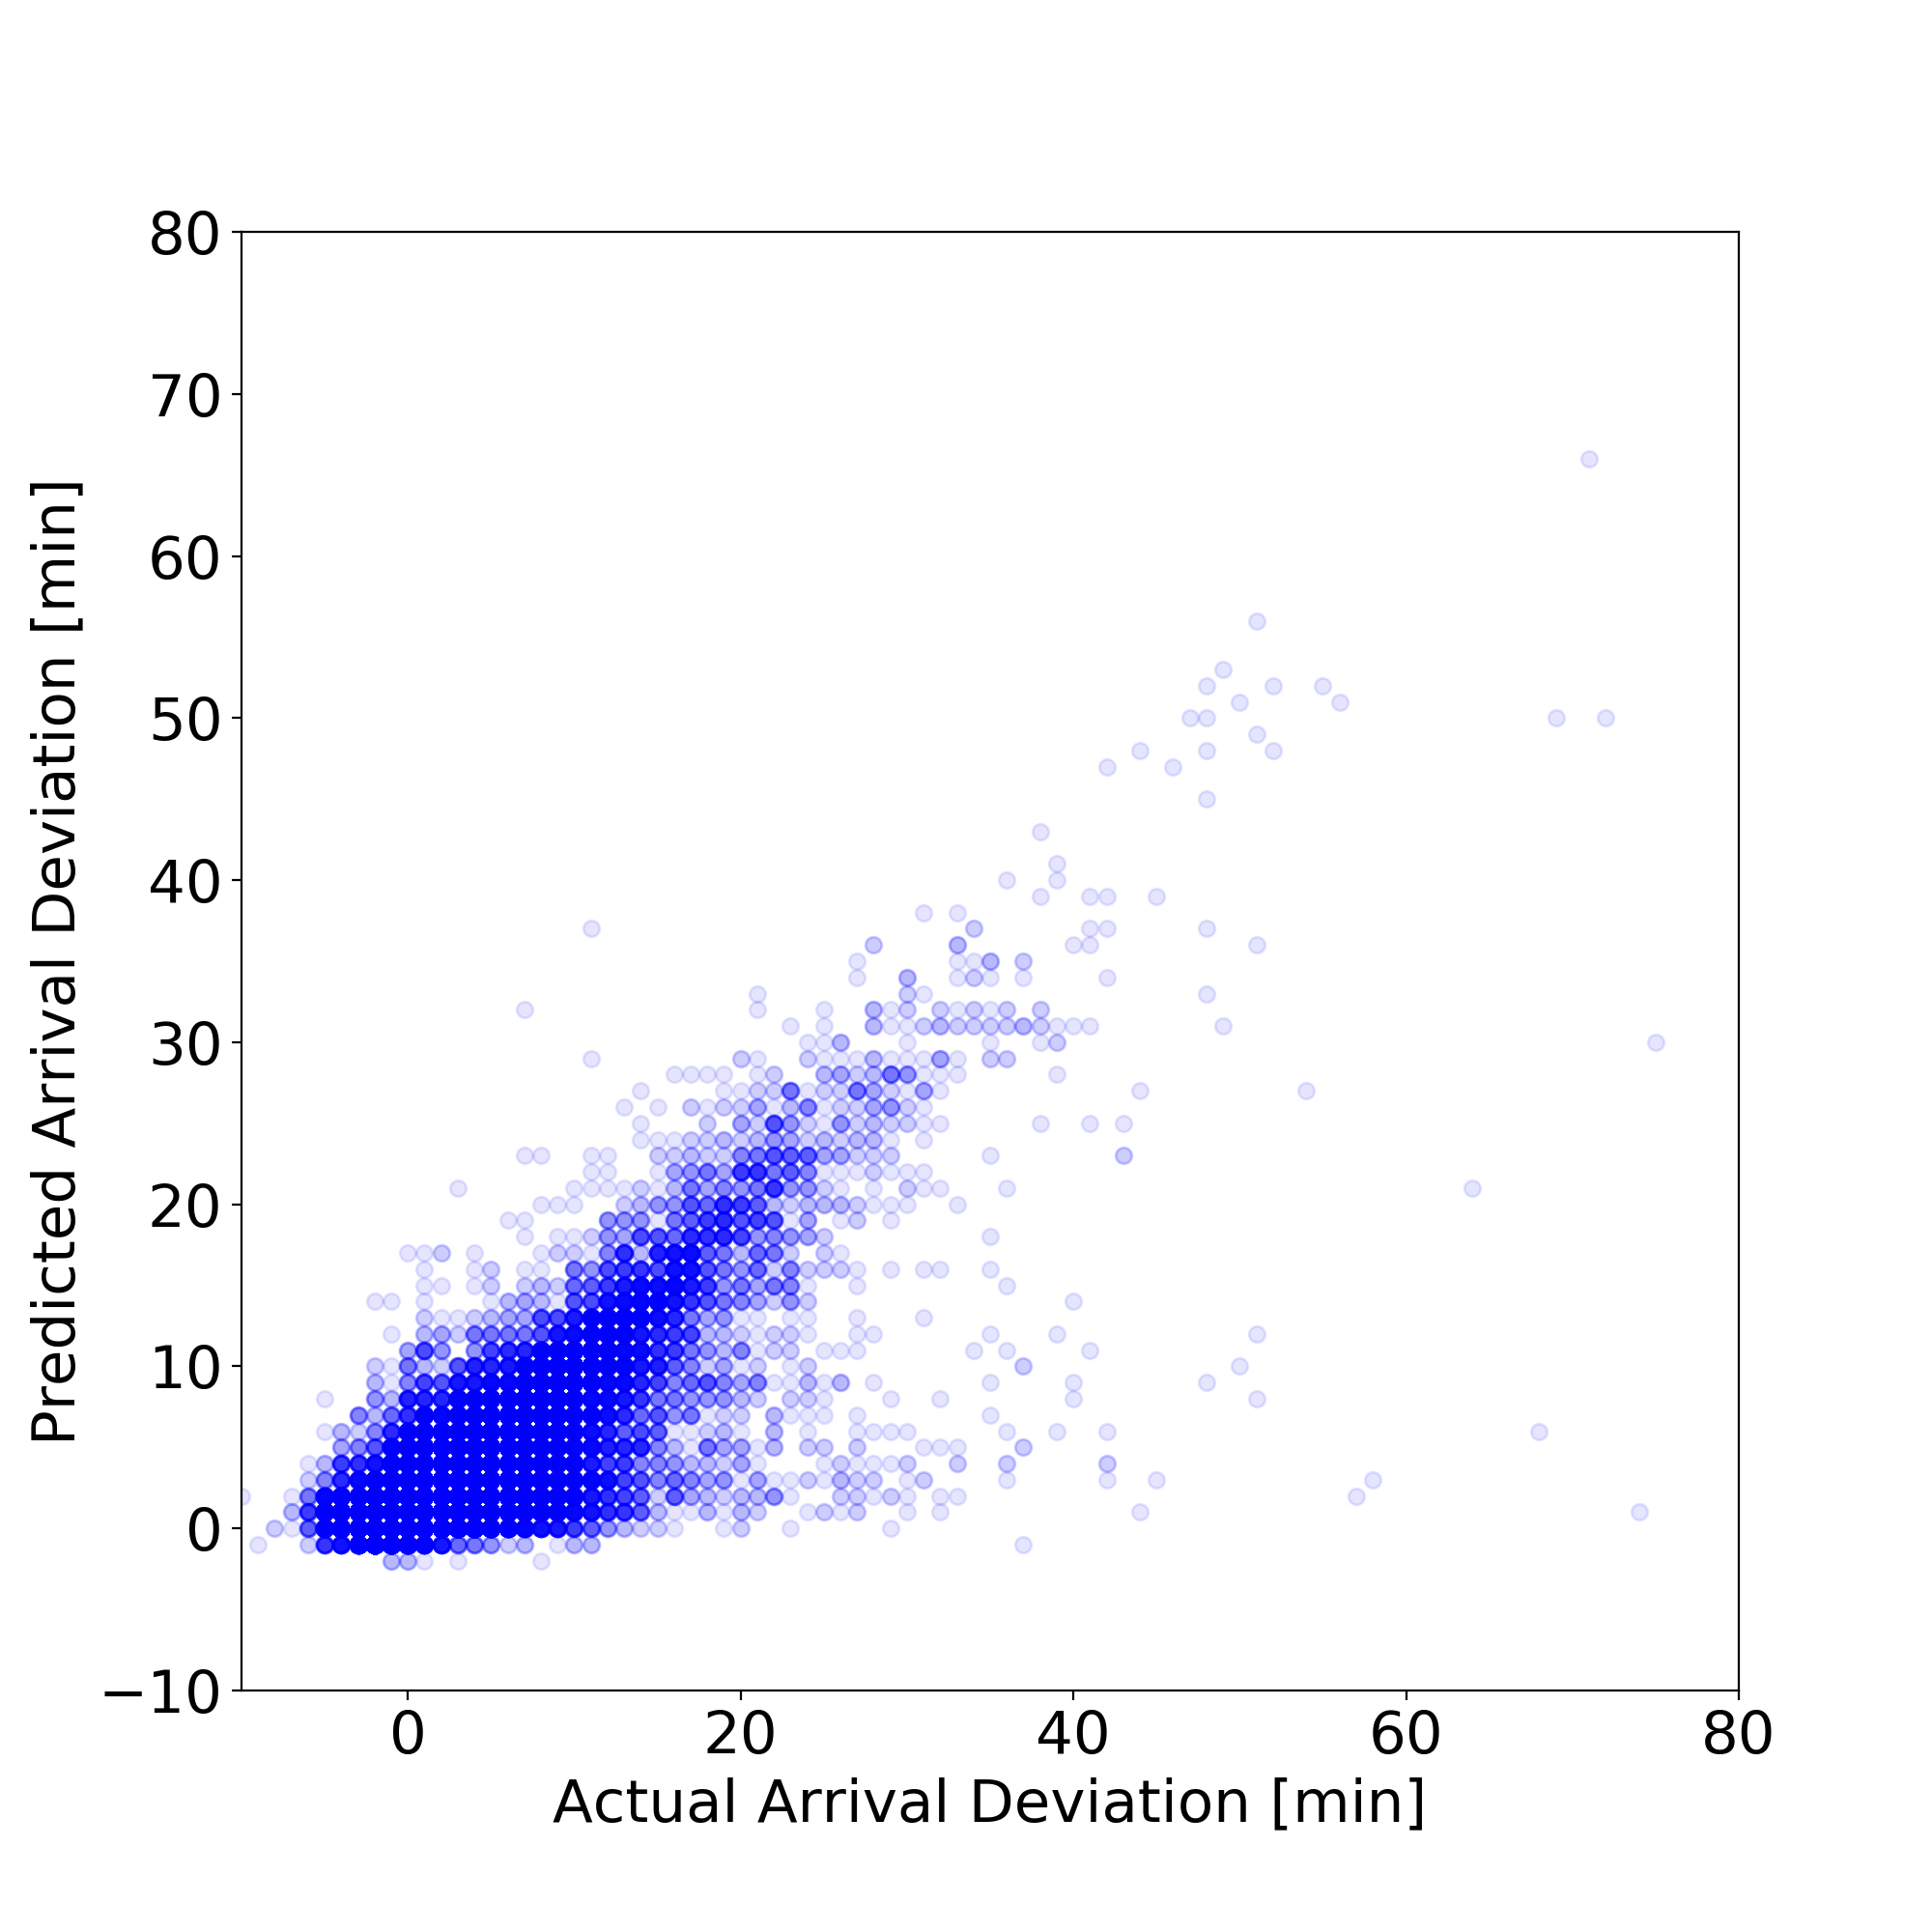
\includegraphics[width=0.5\textwidth]{Images/XGBoost_plot/3_step/3_step_arrival_deviation.png}\label{fig:3_step_arrival_deviation}}
\end{figure}
\begin{figure}[H]
\centering
\subfloat[\tiny{3-Step DNN Deviation from Departure}]{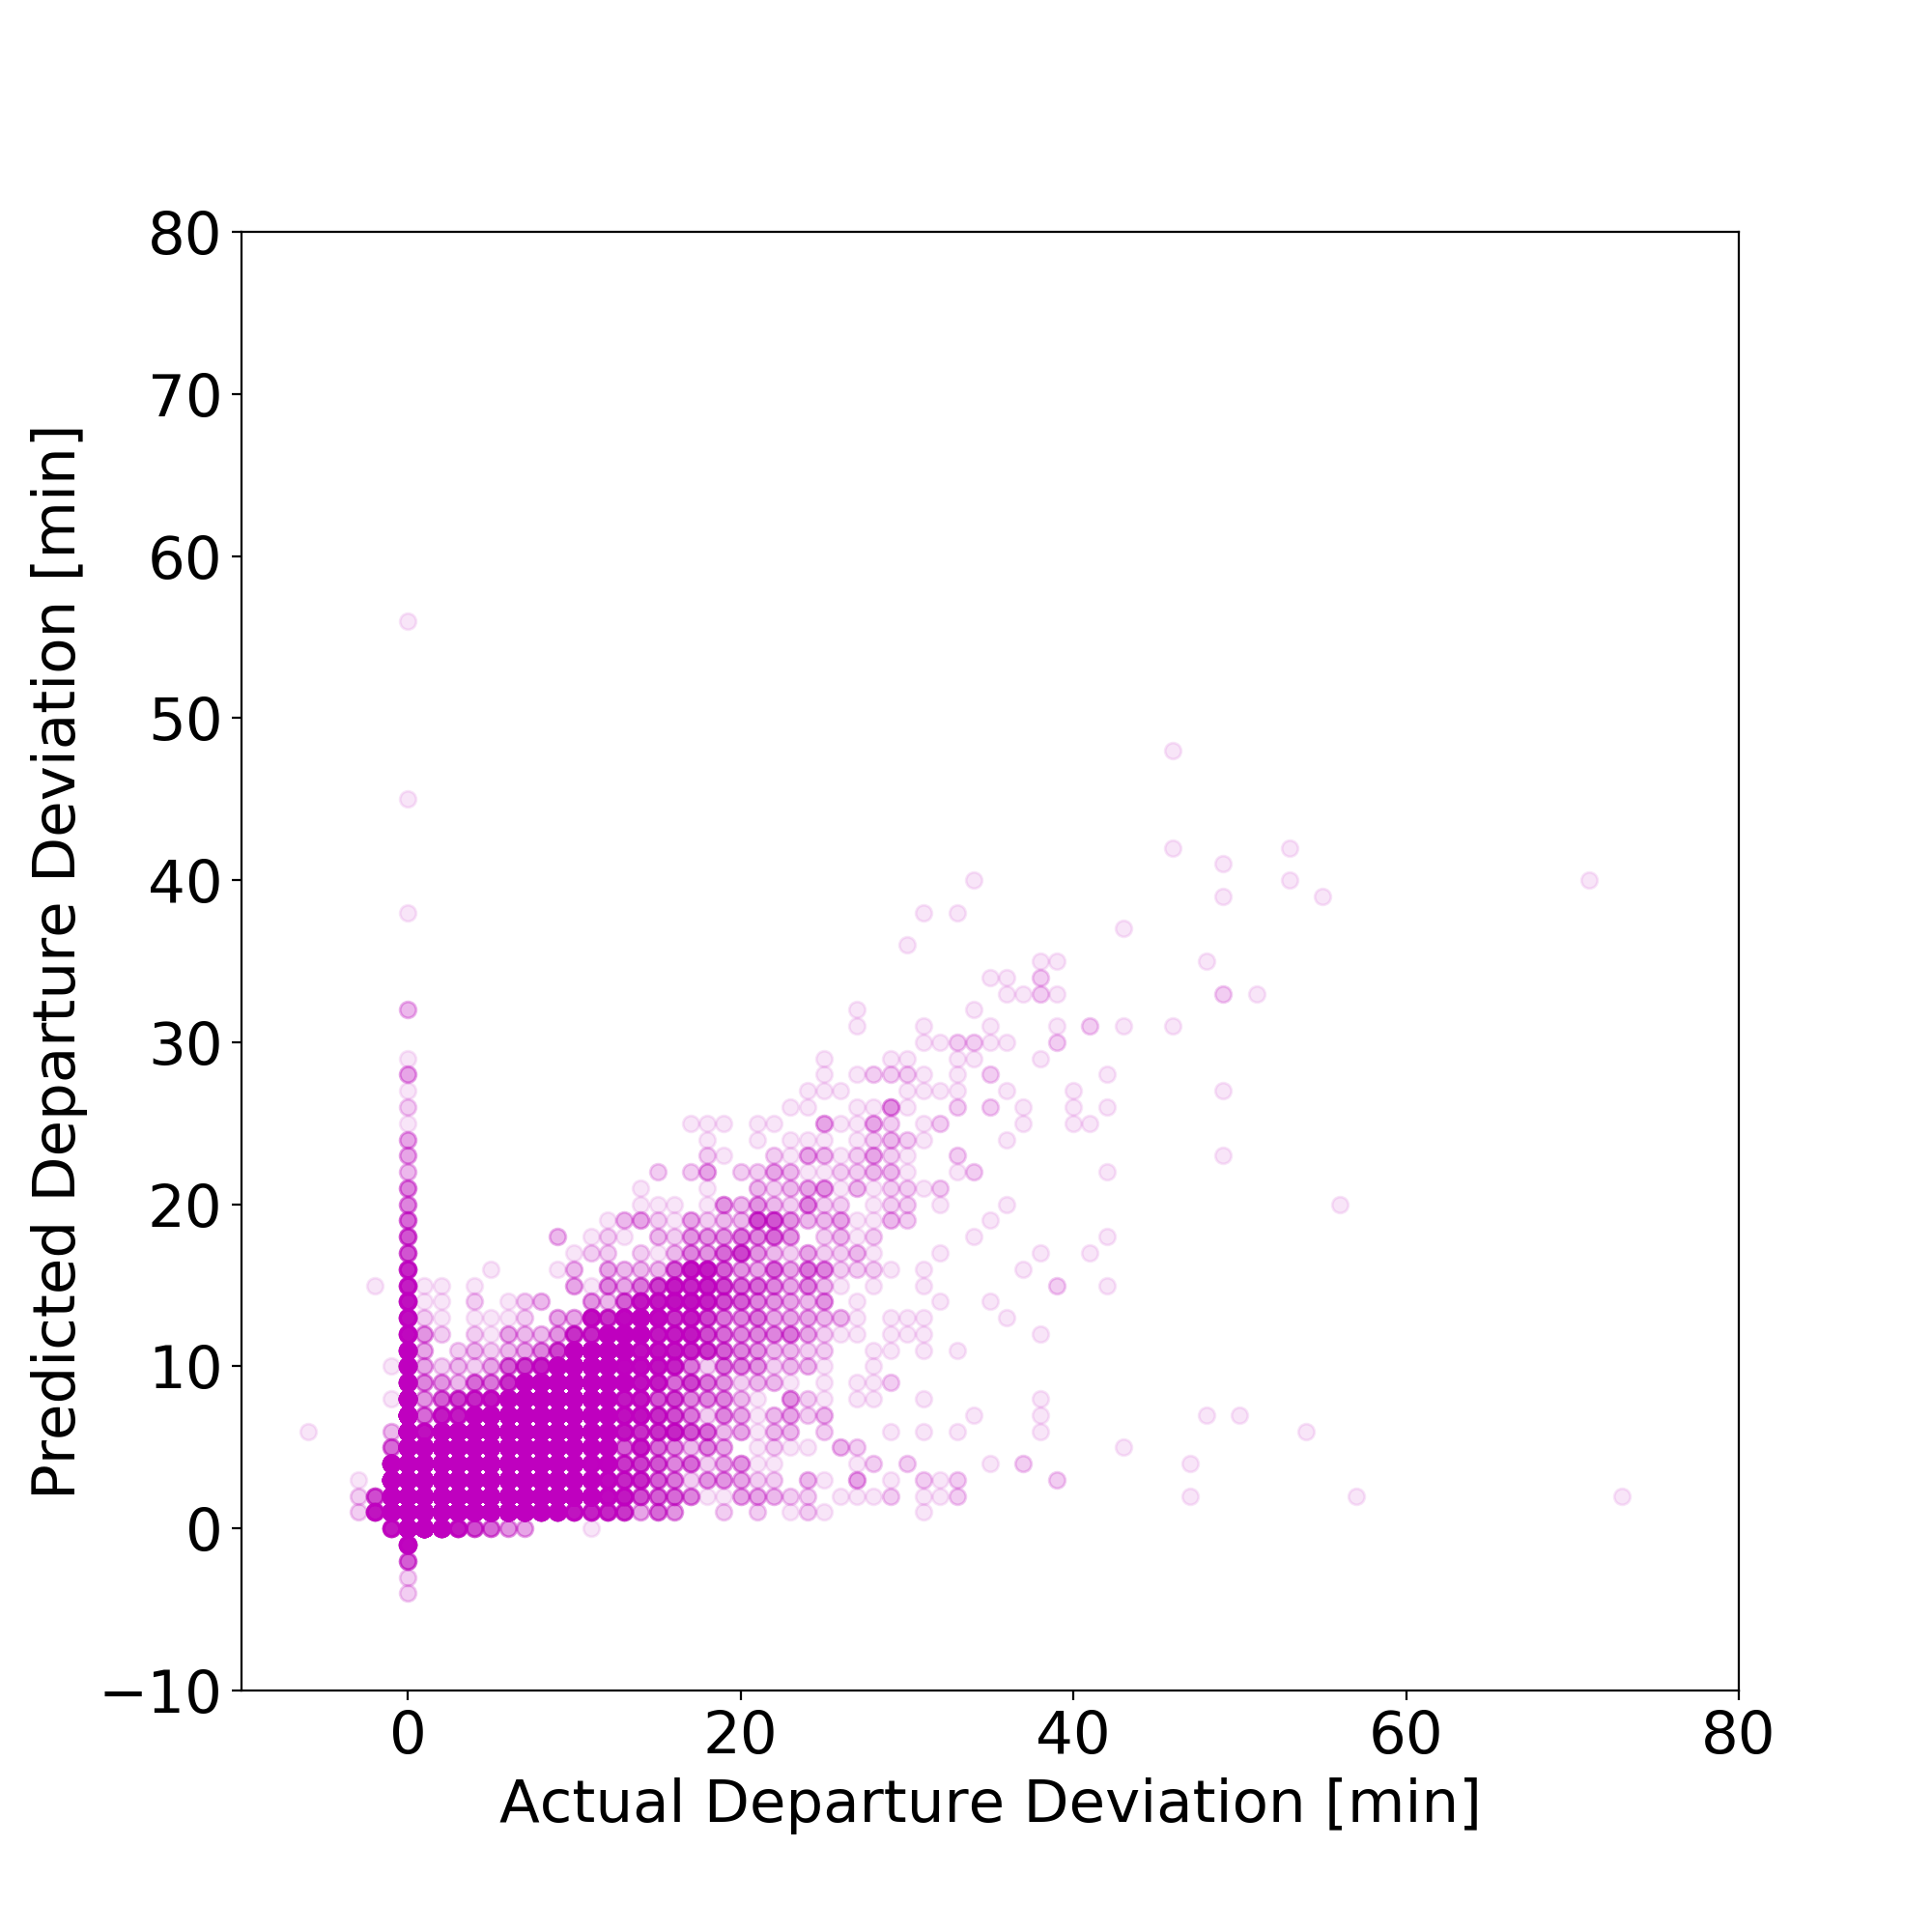
\includegraphics[width=0.5\textwidth]{Images/DNN_plot/3_step/3_step_depature_deviation.png}\label{fig:3_step_depature_deviation}}
\subfloat[\tiny{3-Step XGBoost Deviation from Departure}]{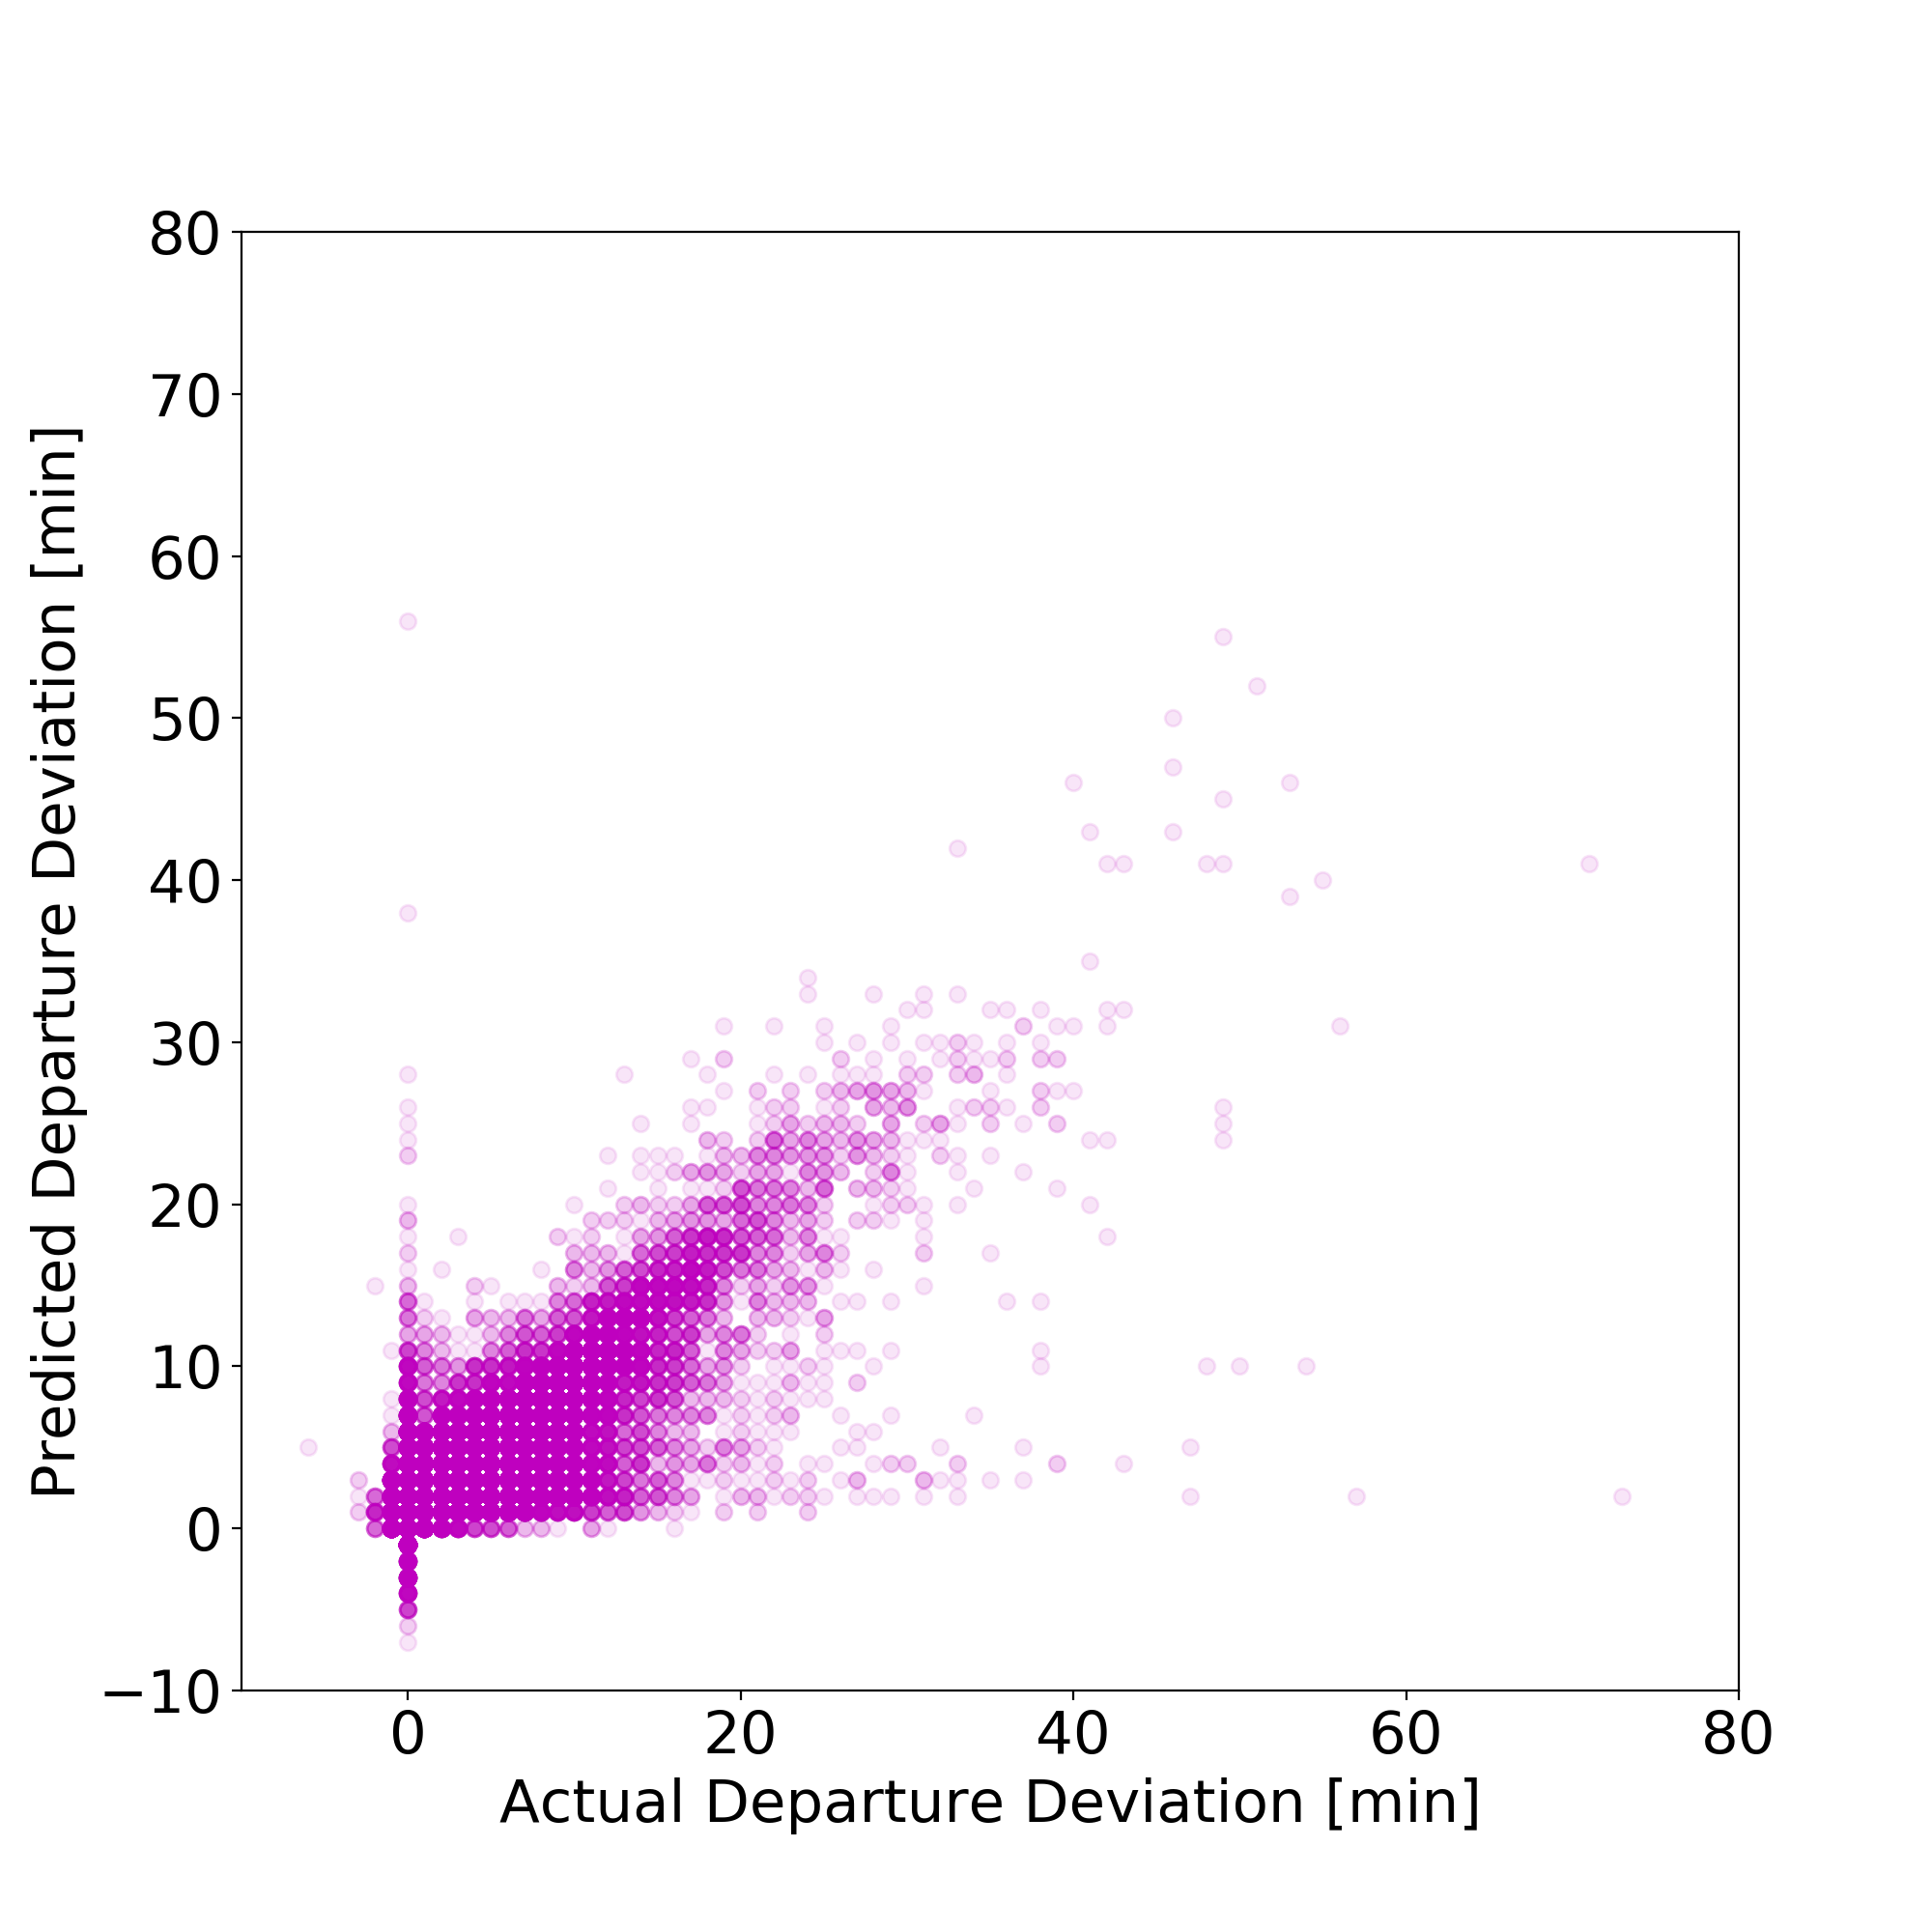
\includegraphics[width=0.5\textwidth]{Images/XGBoost_plot/3_step/3_step_depature_deviation.png}\label{fig:3_step_depature_deviation}}
\end{figure}
\begin{figure}[H]
\centering
\subfloat[\tiny{3-Step DNN Travel Time}]{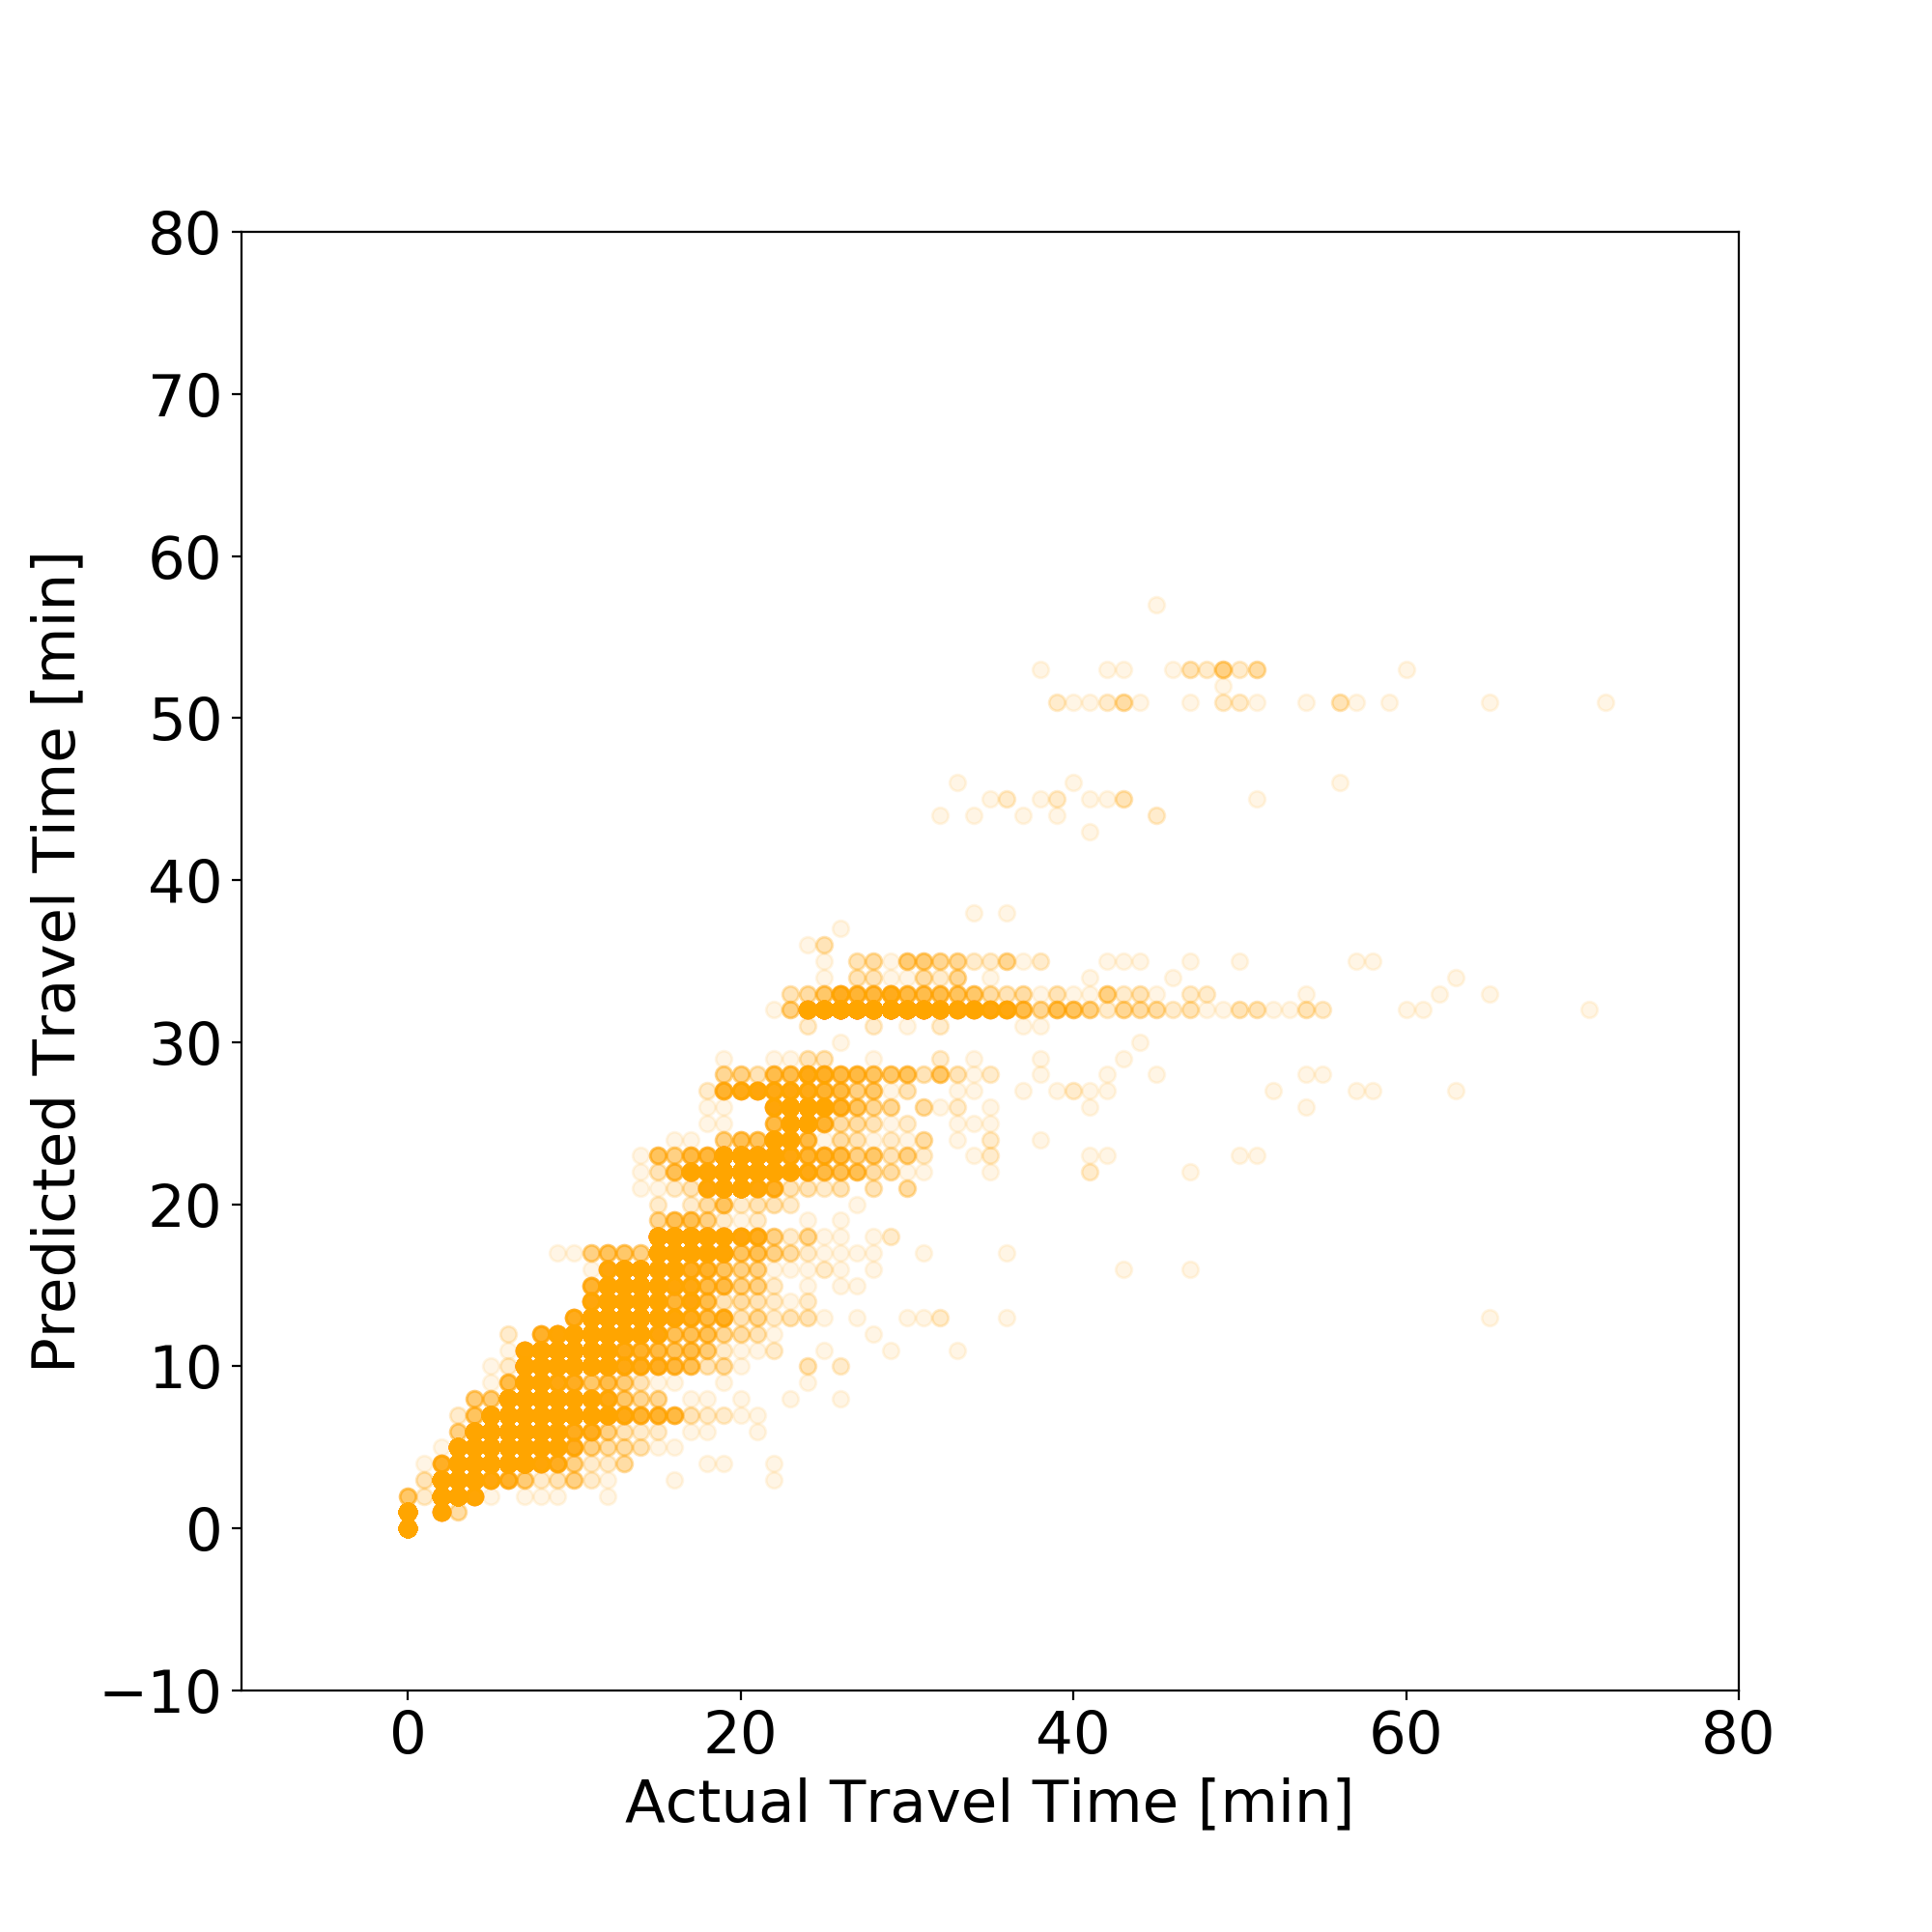
\includegraphics[width=0.5\textwidth]{Images/DNN_plot/3_step/3_step_travel_time.png}\label{fig:3_step_travel_time}}
\subfloat[\tiny{3-Step XGBoost Travel Time}]{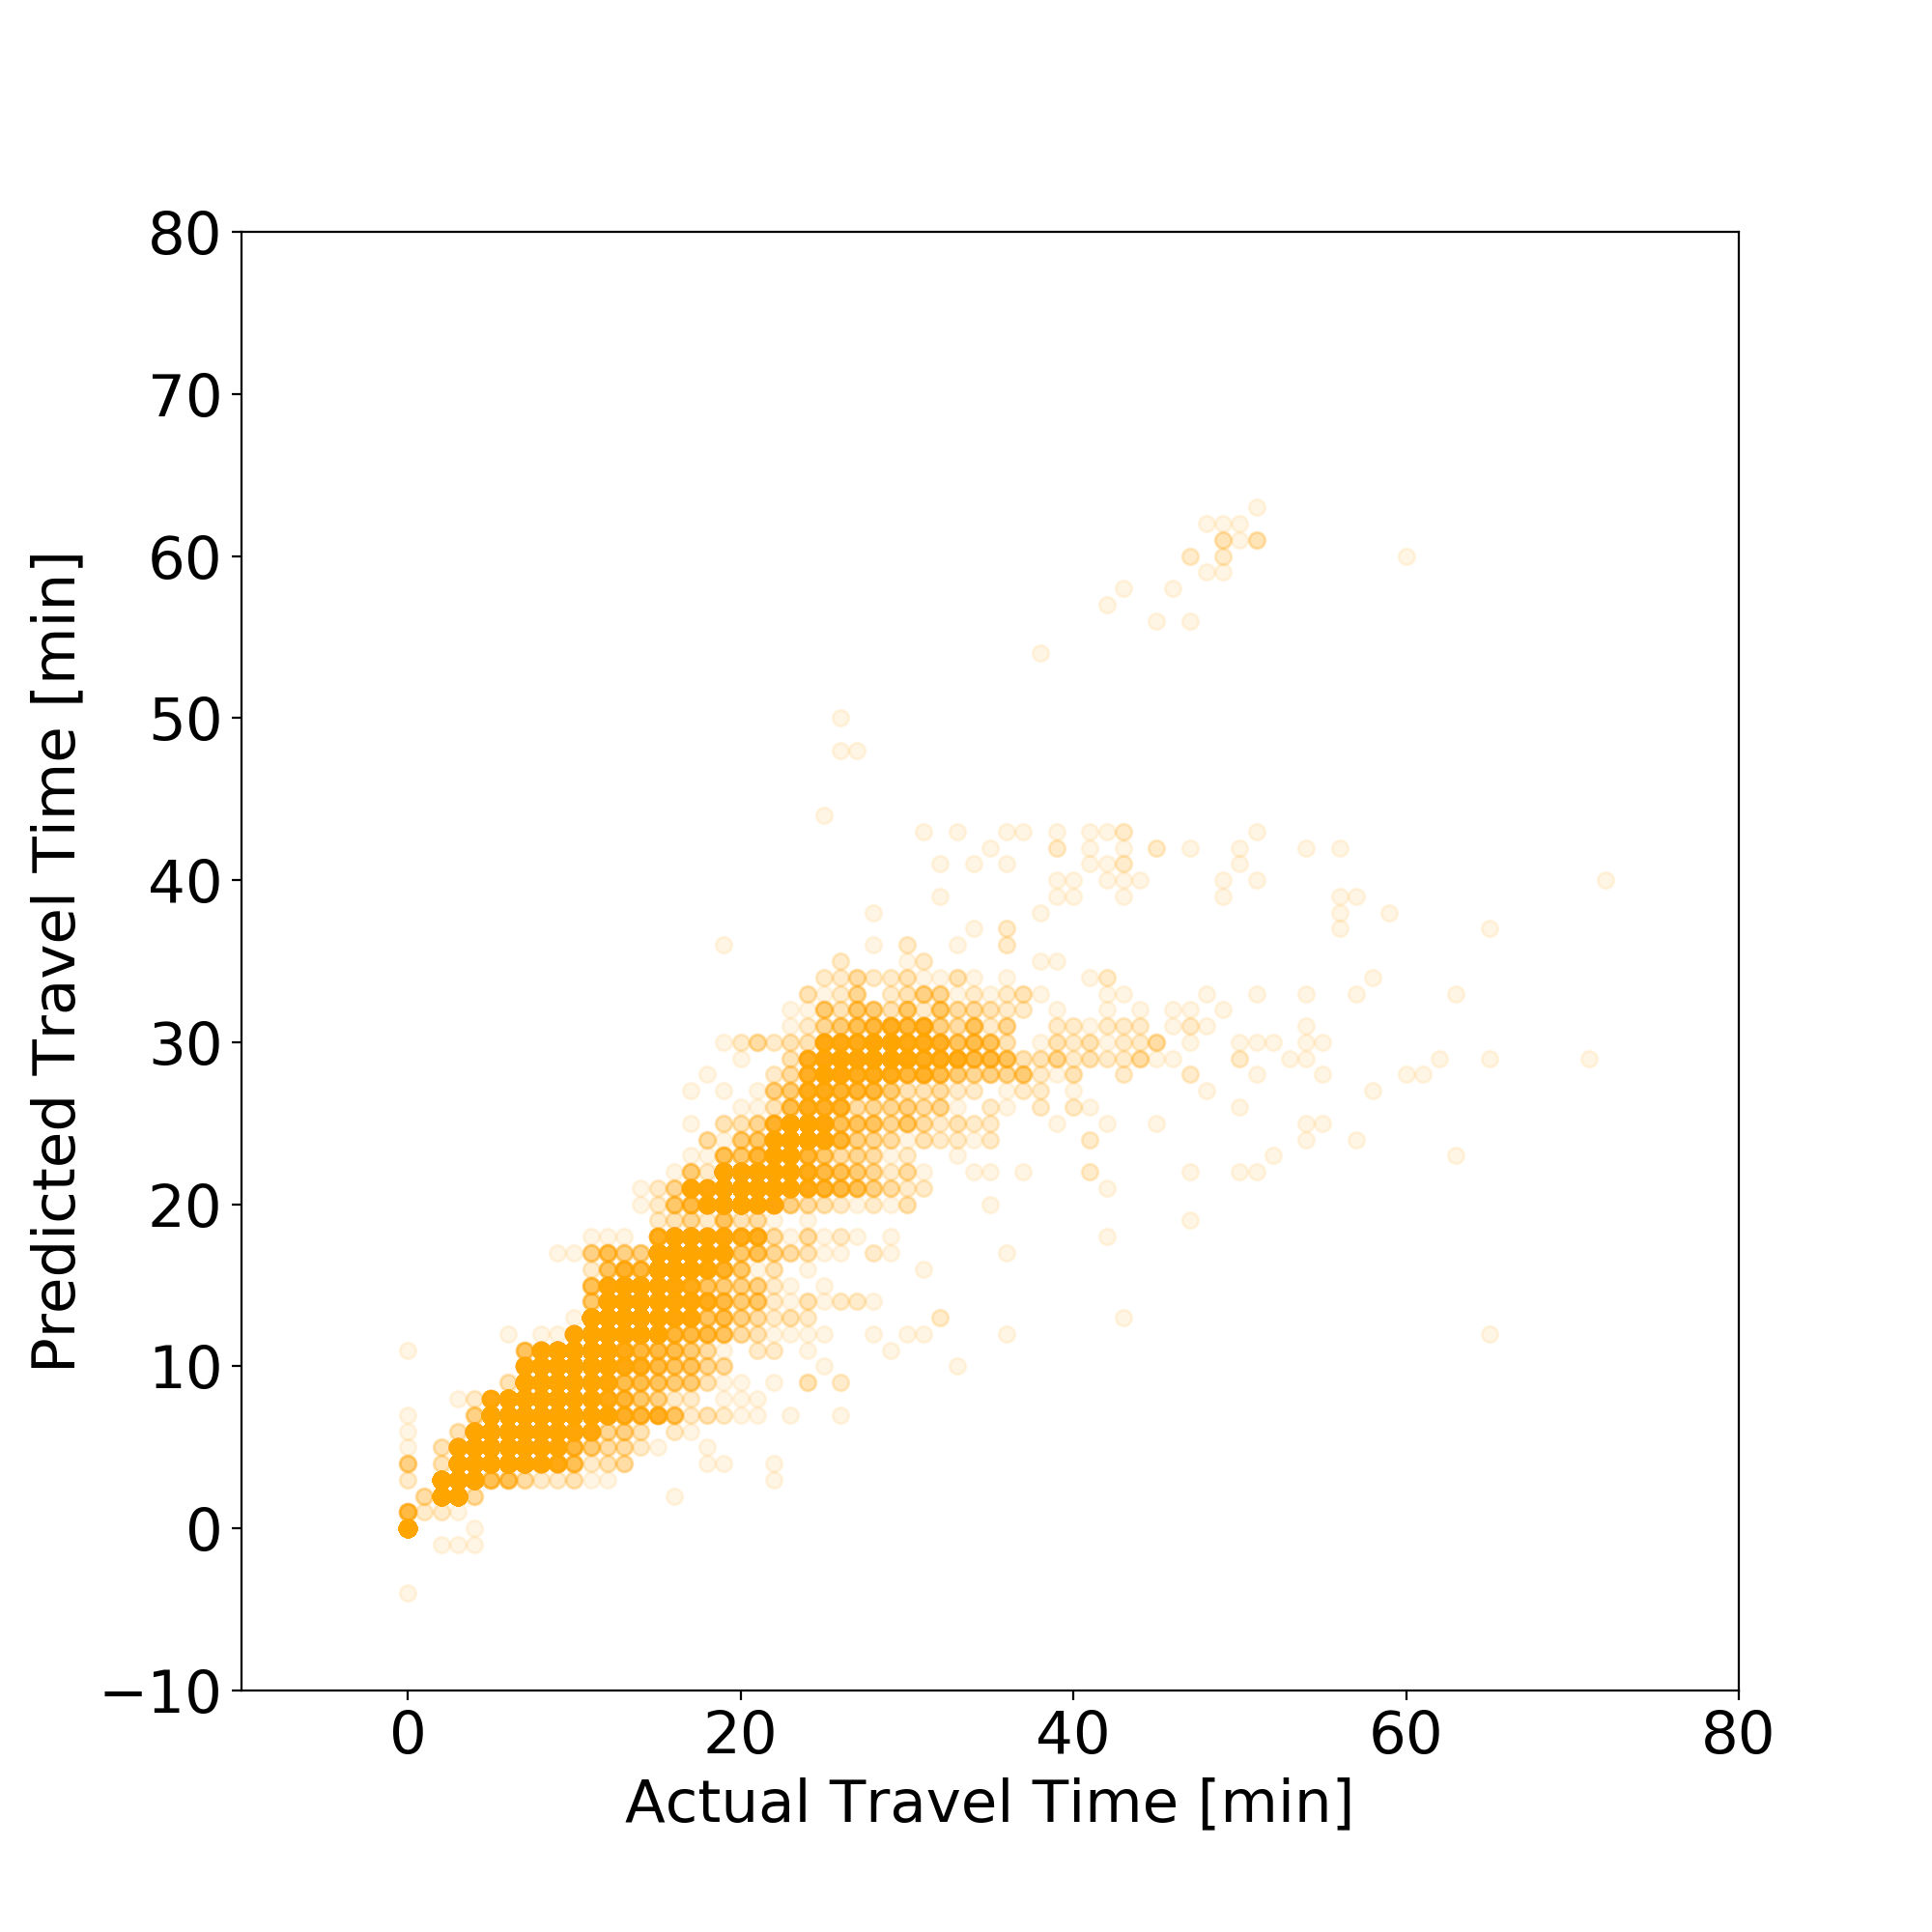
\includegraphics[width=0.5\textwidth]{Images/XGBoost_plot/3_step/3_step_travel_time.png}\label{fig:3_step_travel_time}}
\end{figure}
\begin{figure}[H]
\centering
\subfloat[\tiny{3-Step DNN Dwell Time}]{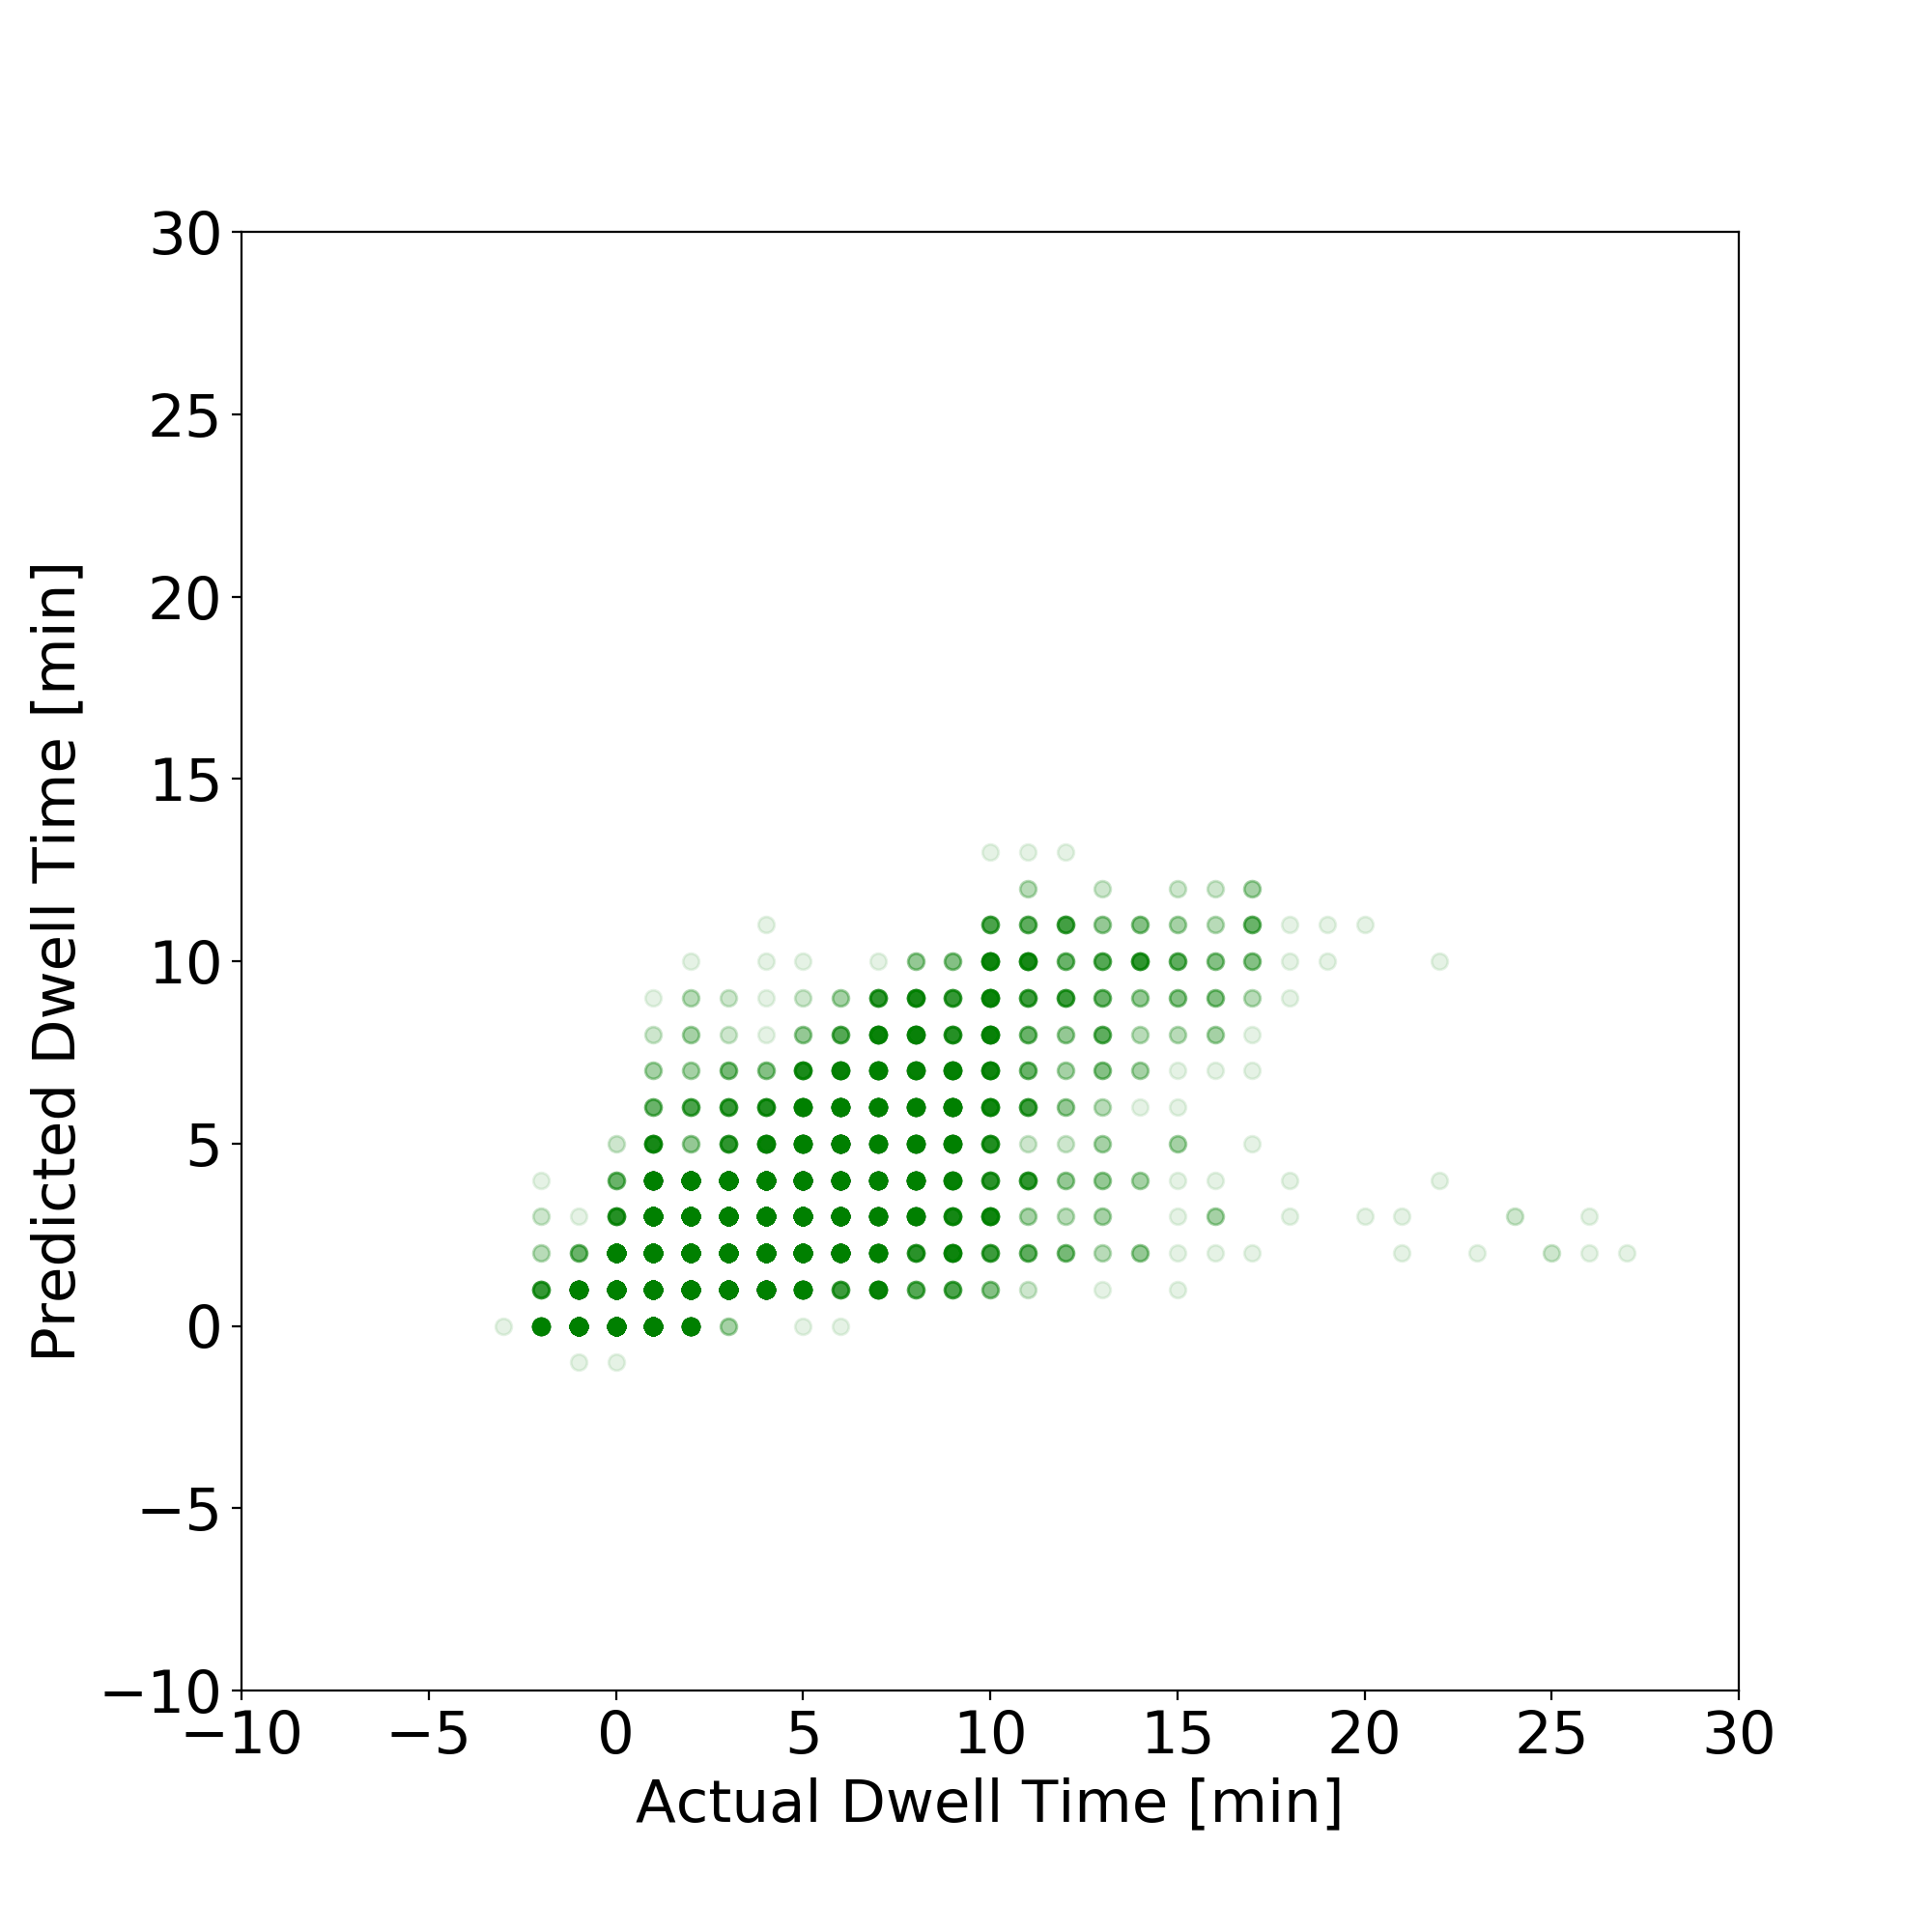
\includegraphics[width=0.5\textwidth]{Images/DNN_plot/3_step/3_step_dwell_time.png}\label{fig:3_step_dwell_time}}
\subfloat[\tiny{3-Step XGBoost Dwell Time}]{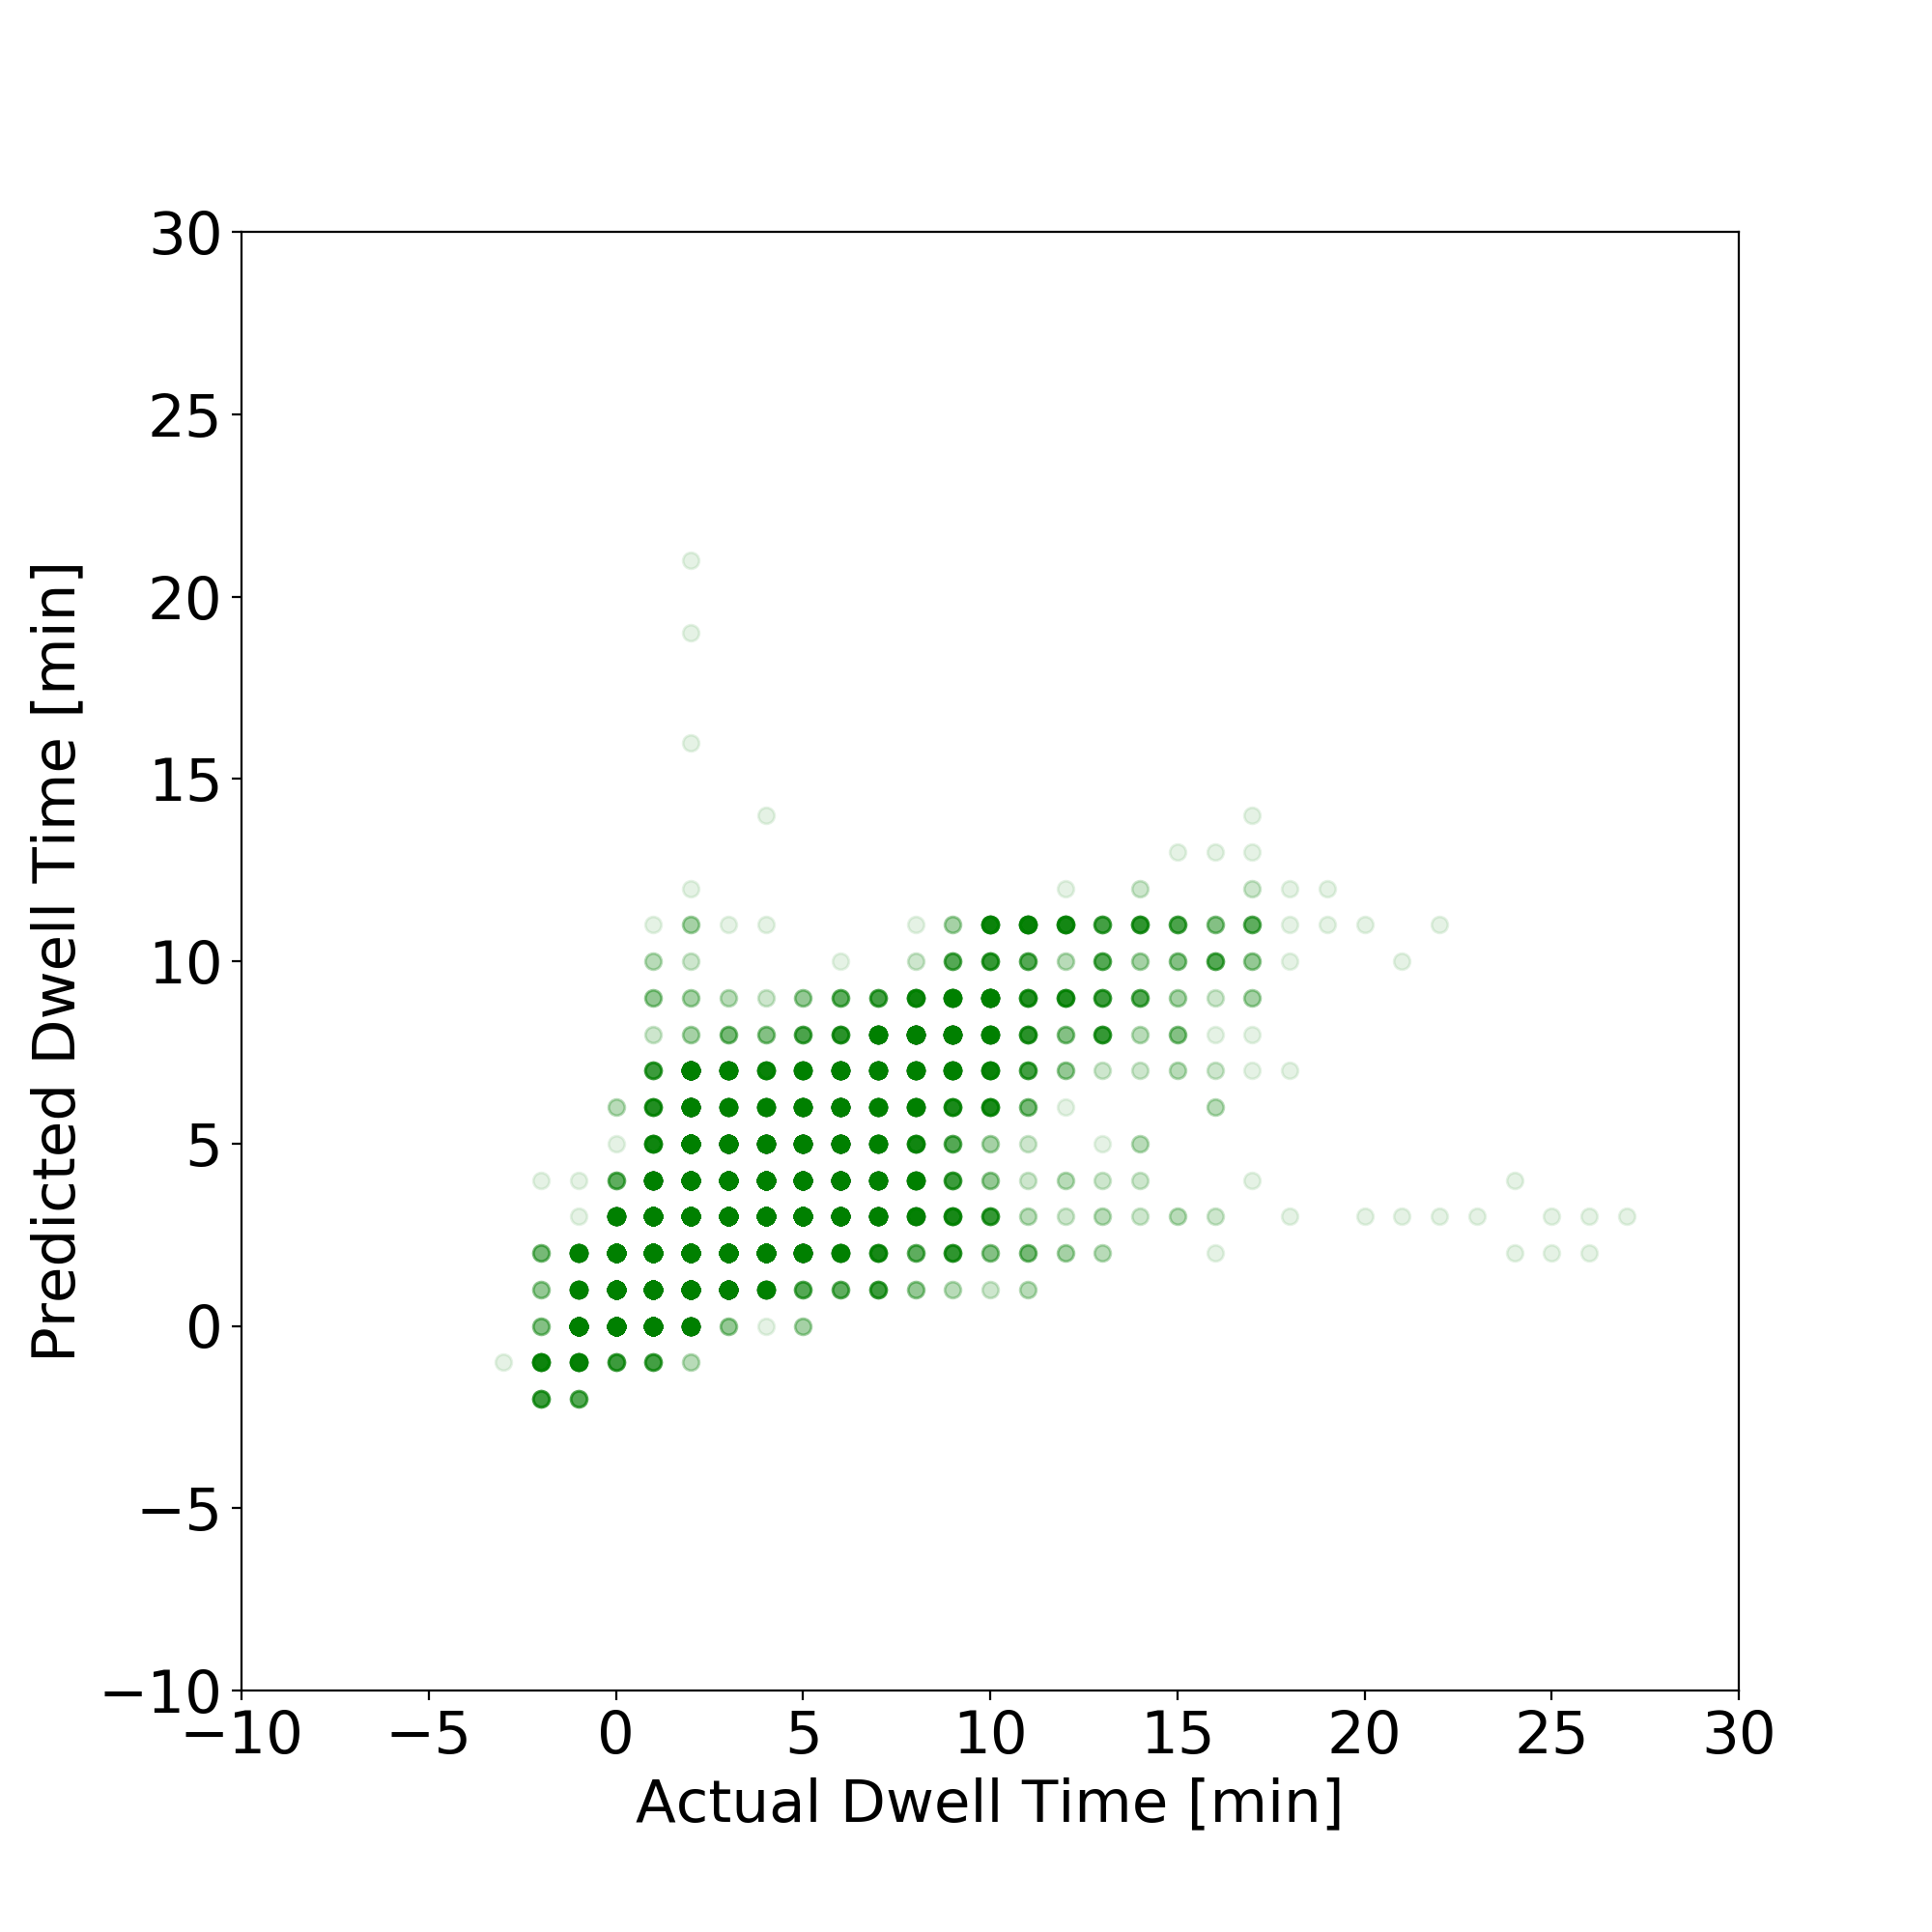
\includegraphics[width=0.5\textwidth]{Images/XGBoost_plot/3_step/3_step_dwell_time.png}\label{fig:3_step_dwell_time}}
\end{figure}

\begin{figure}[H]
\centering
\subfloat[\tiny{4-Step DNN Deviation from Arrival}]{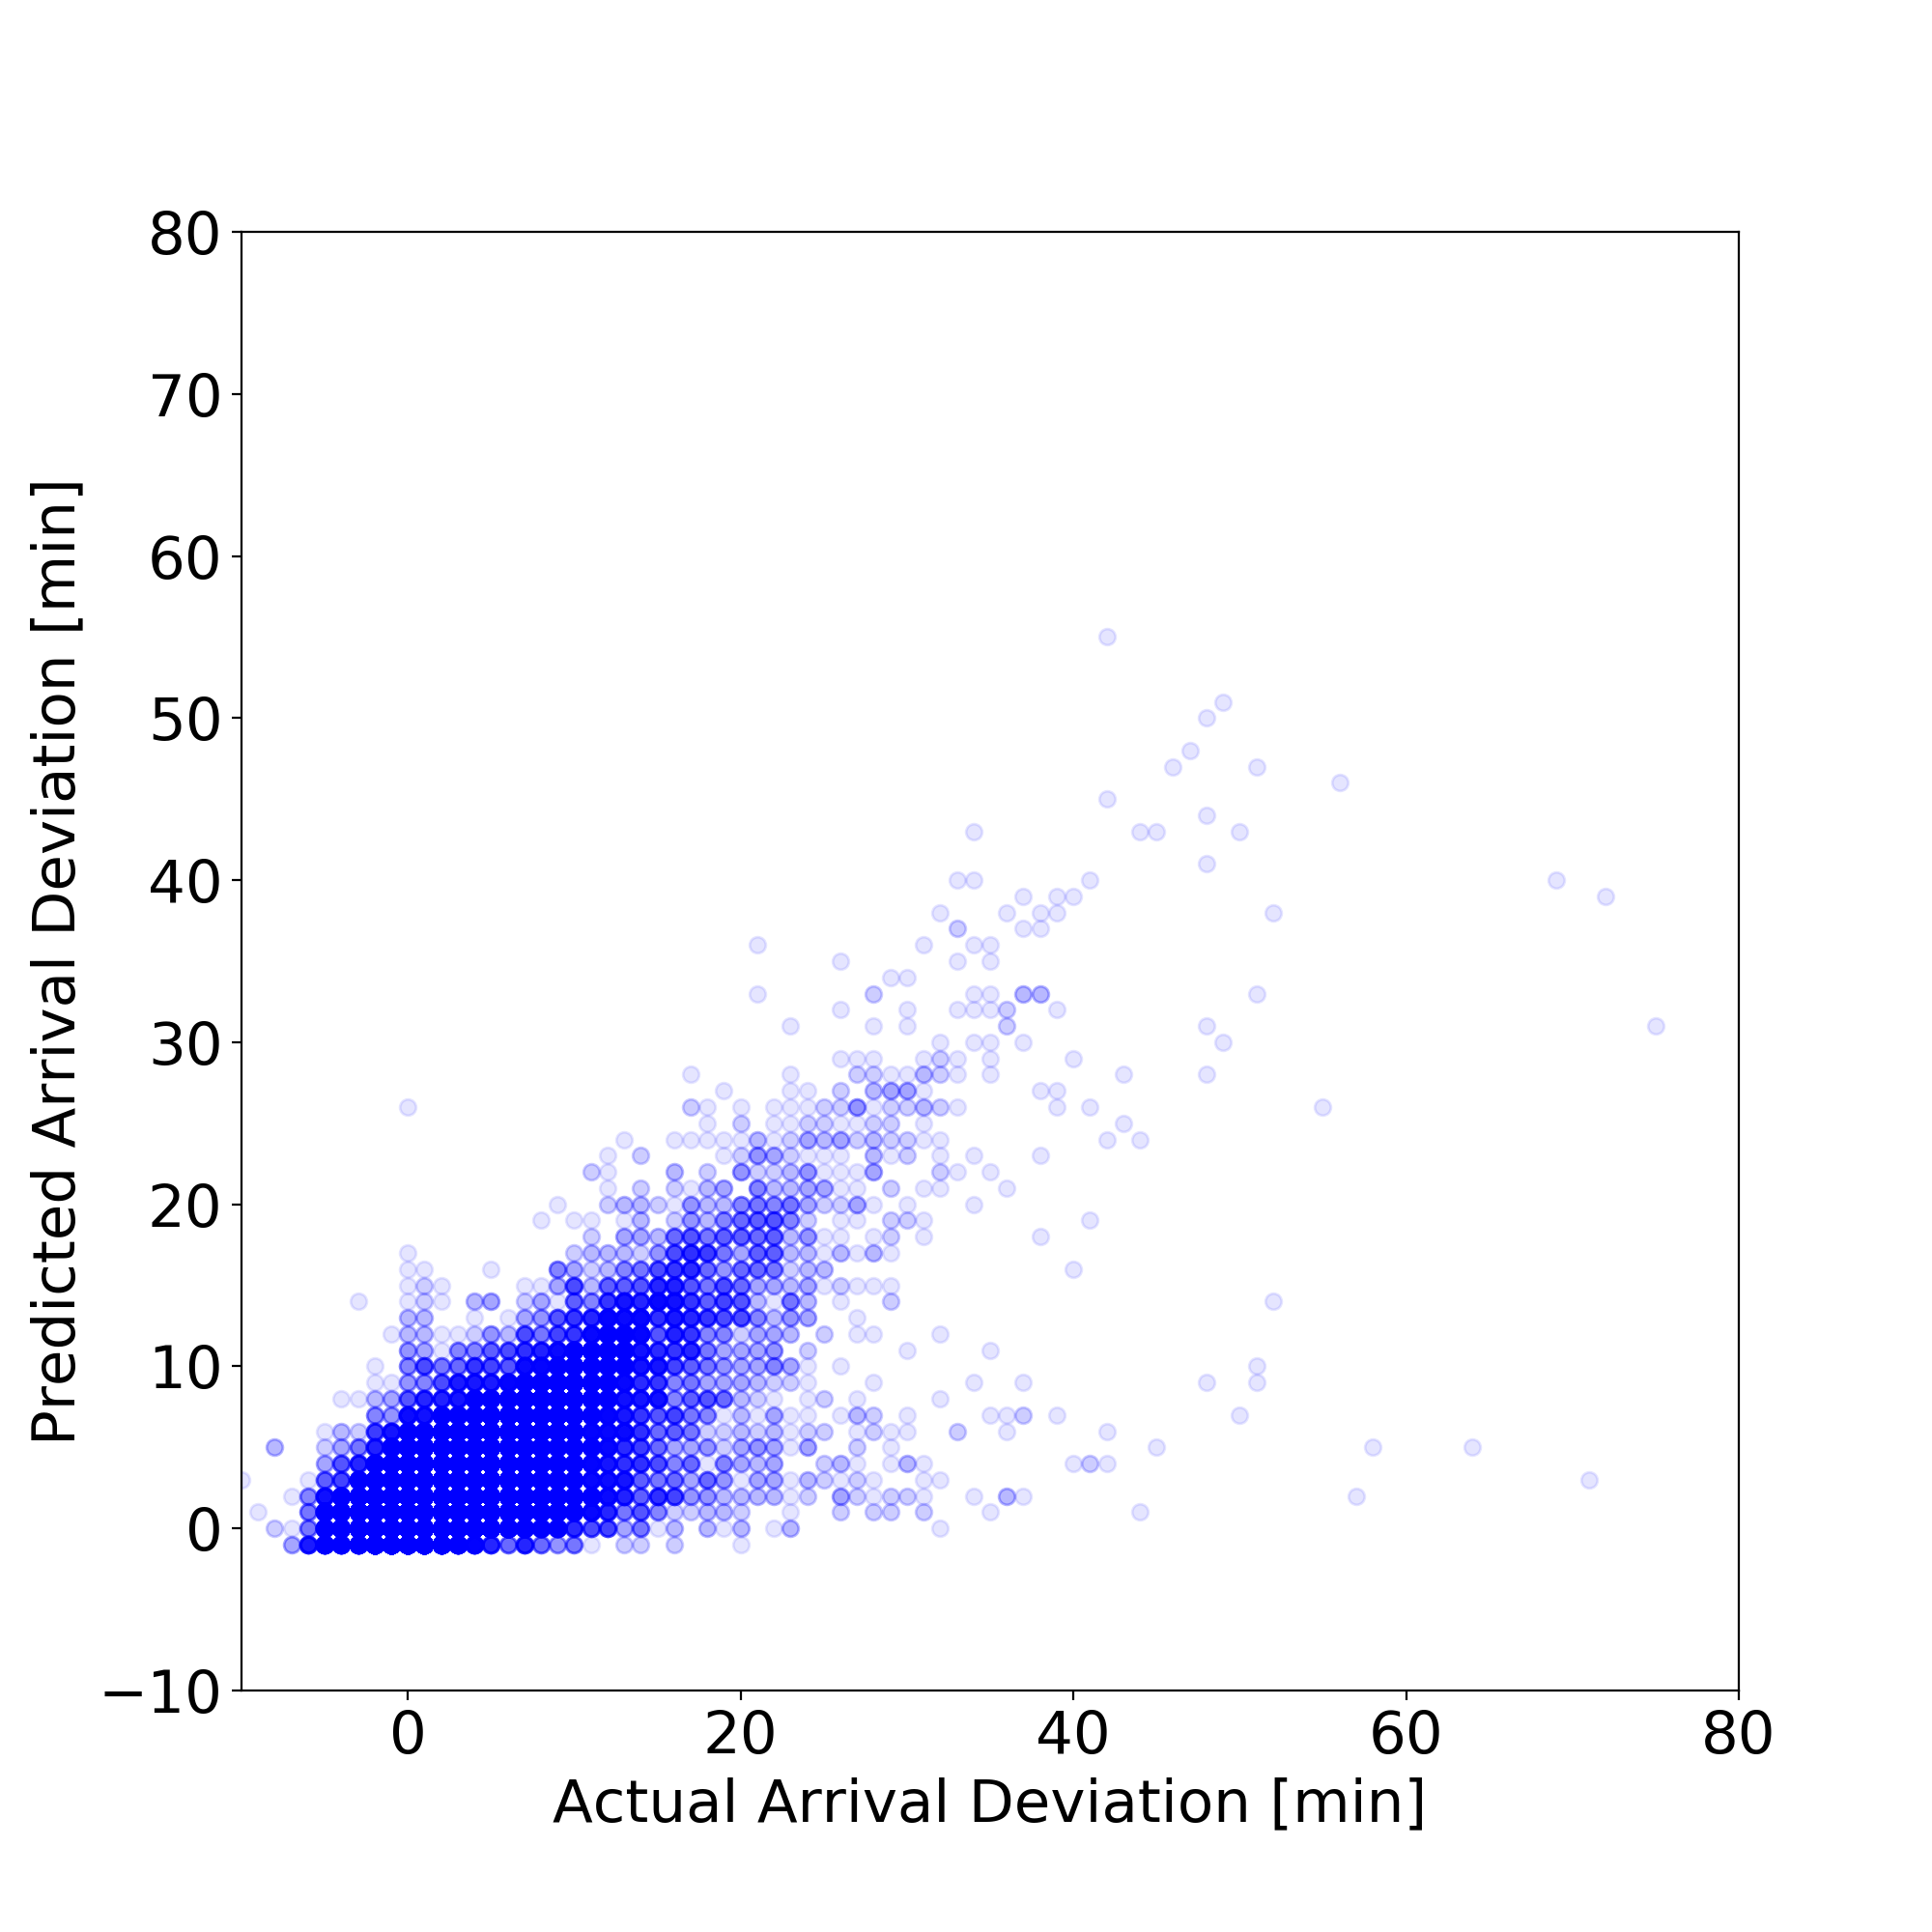
\includegraphics[width=0.5\textwidth]{Images/DNN_plot/4_step/4_step_arrival_deviation.png}\label{fig:4_step_arrival_deviation}}
\subfloat[\tiny{4-Step XGBoost Deviation from Arrival}]{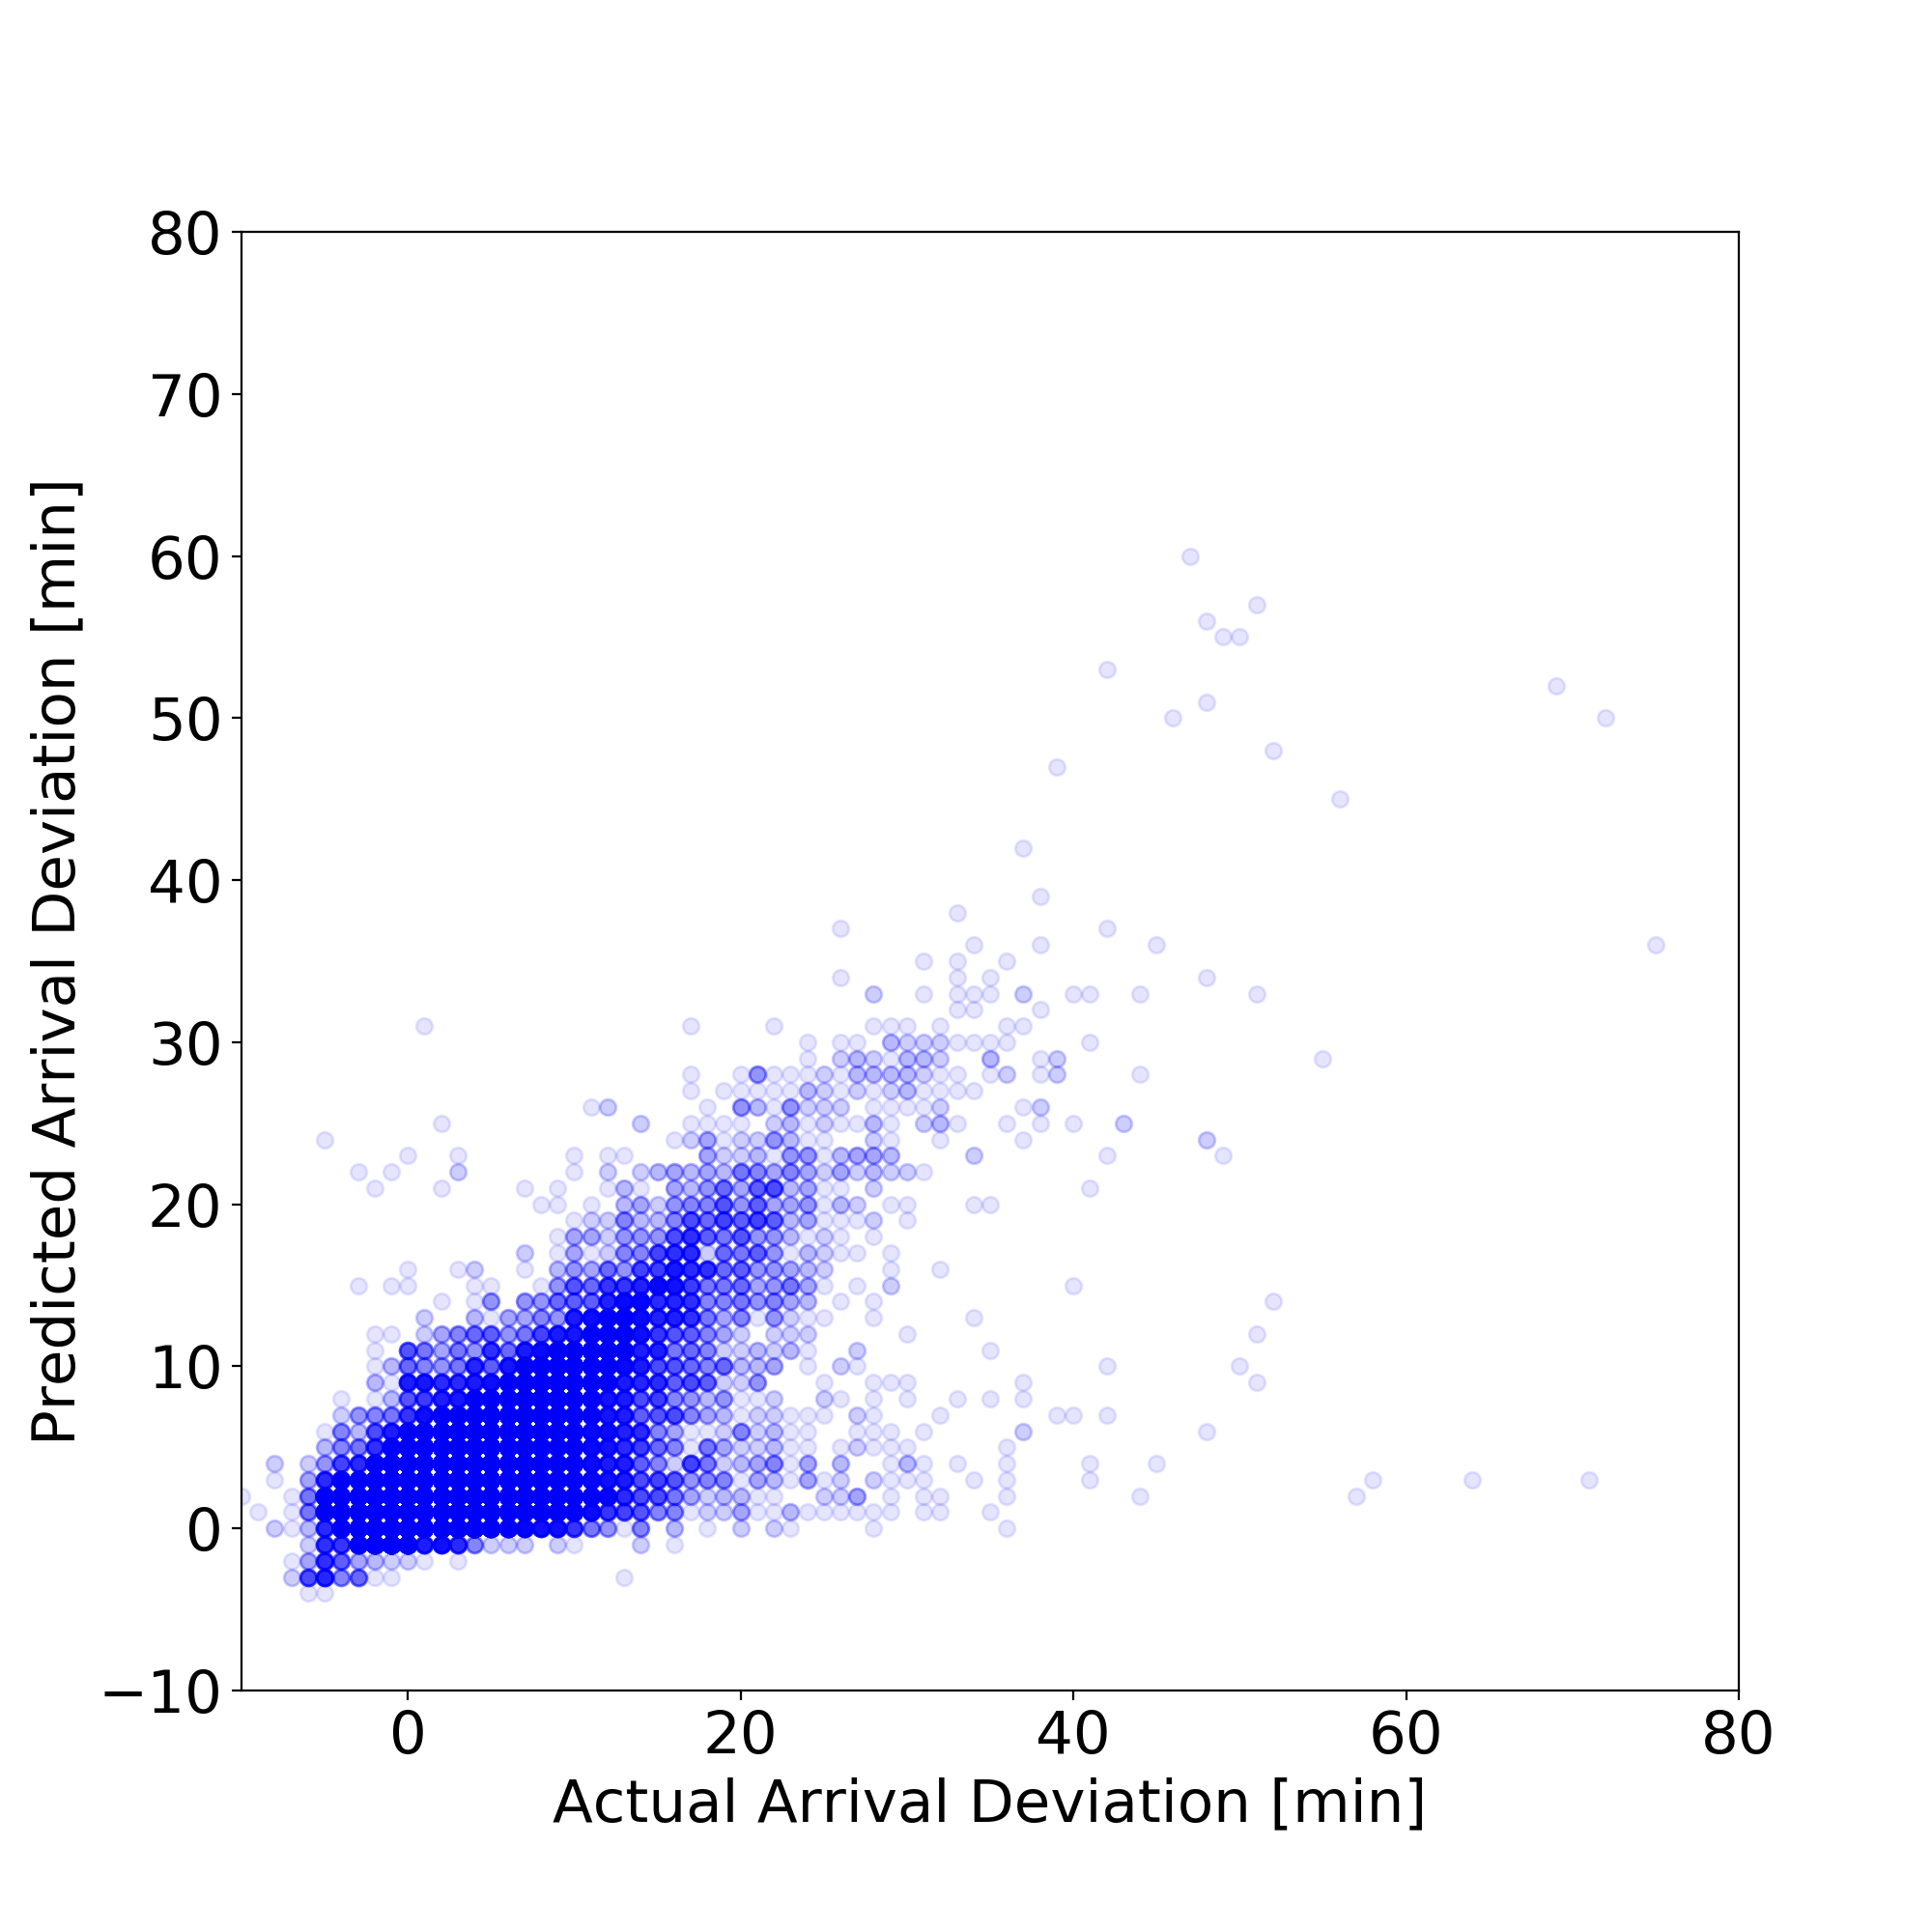
\includegraphics[width=0.5\textwidth]{Images/XGBoost_plot/4_step/4_step_arrival_deviation.png}\label{fig:4_step_arrival_deviation}}
\end{figure}
\begin{figure}[H]
\centering
\subfloat[\tiny{4-Step DNN Deviation from Departure}]{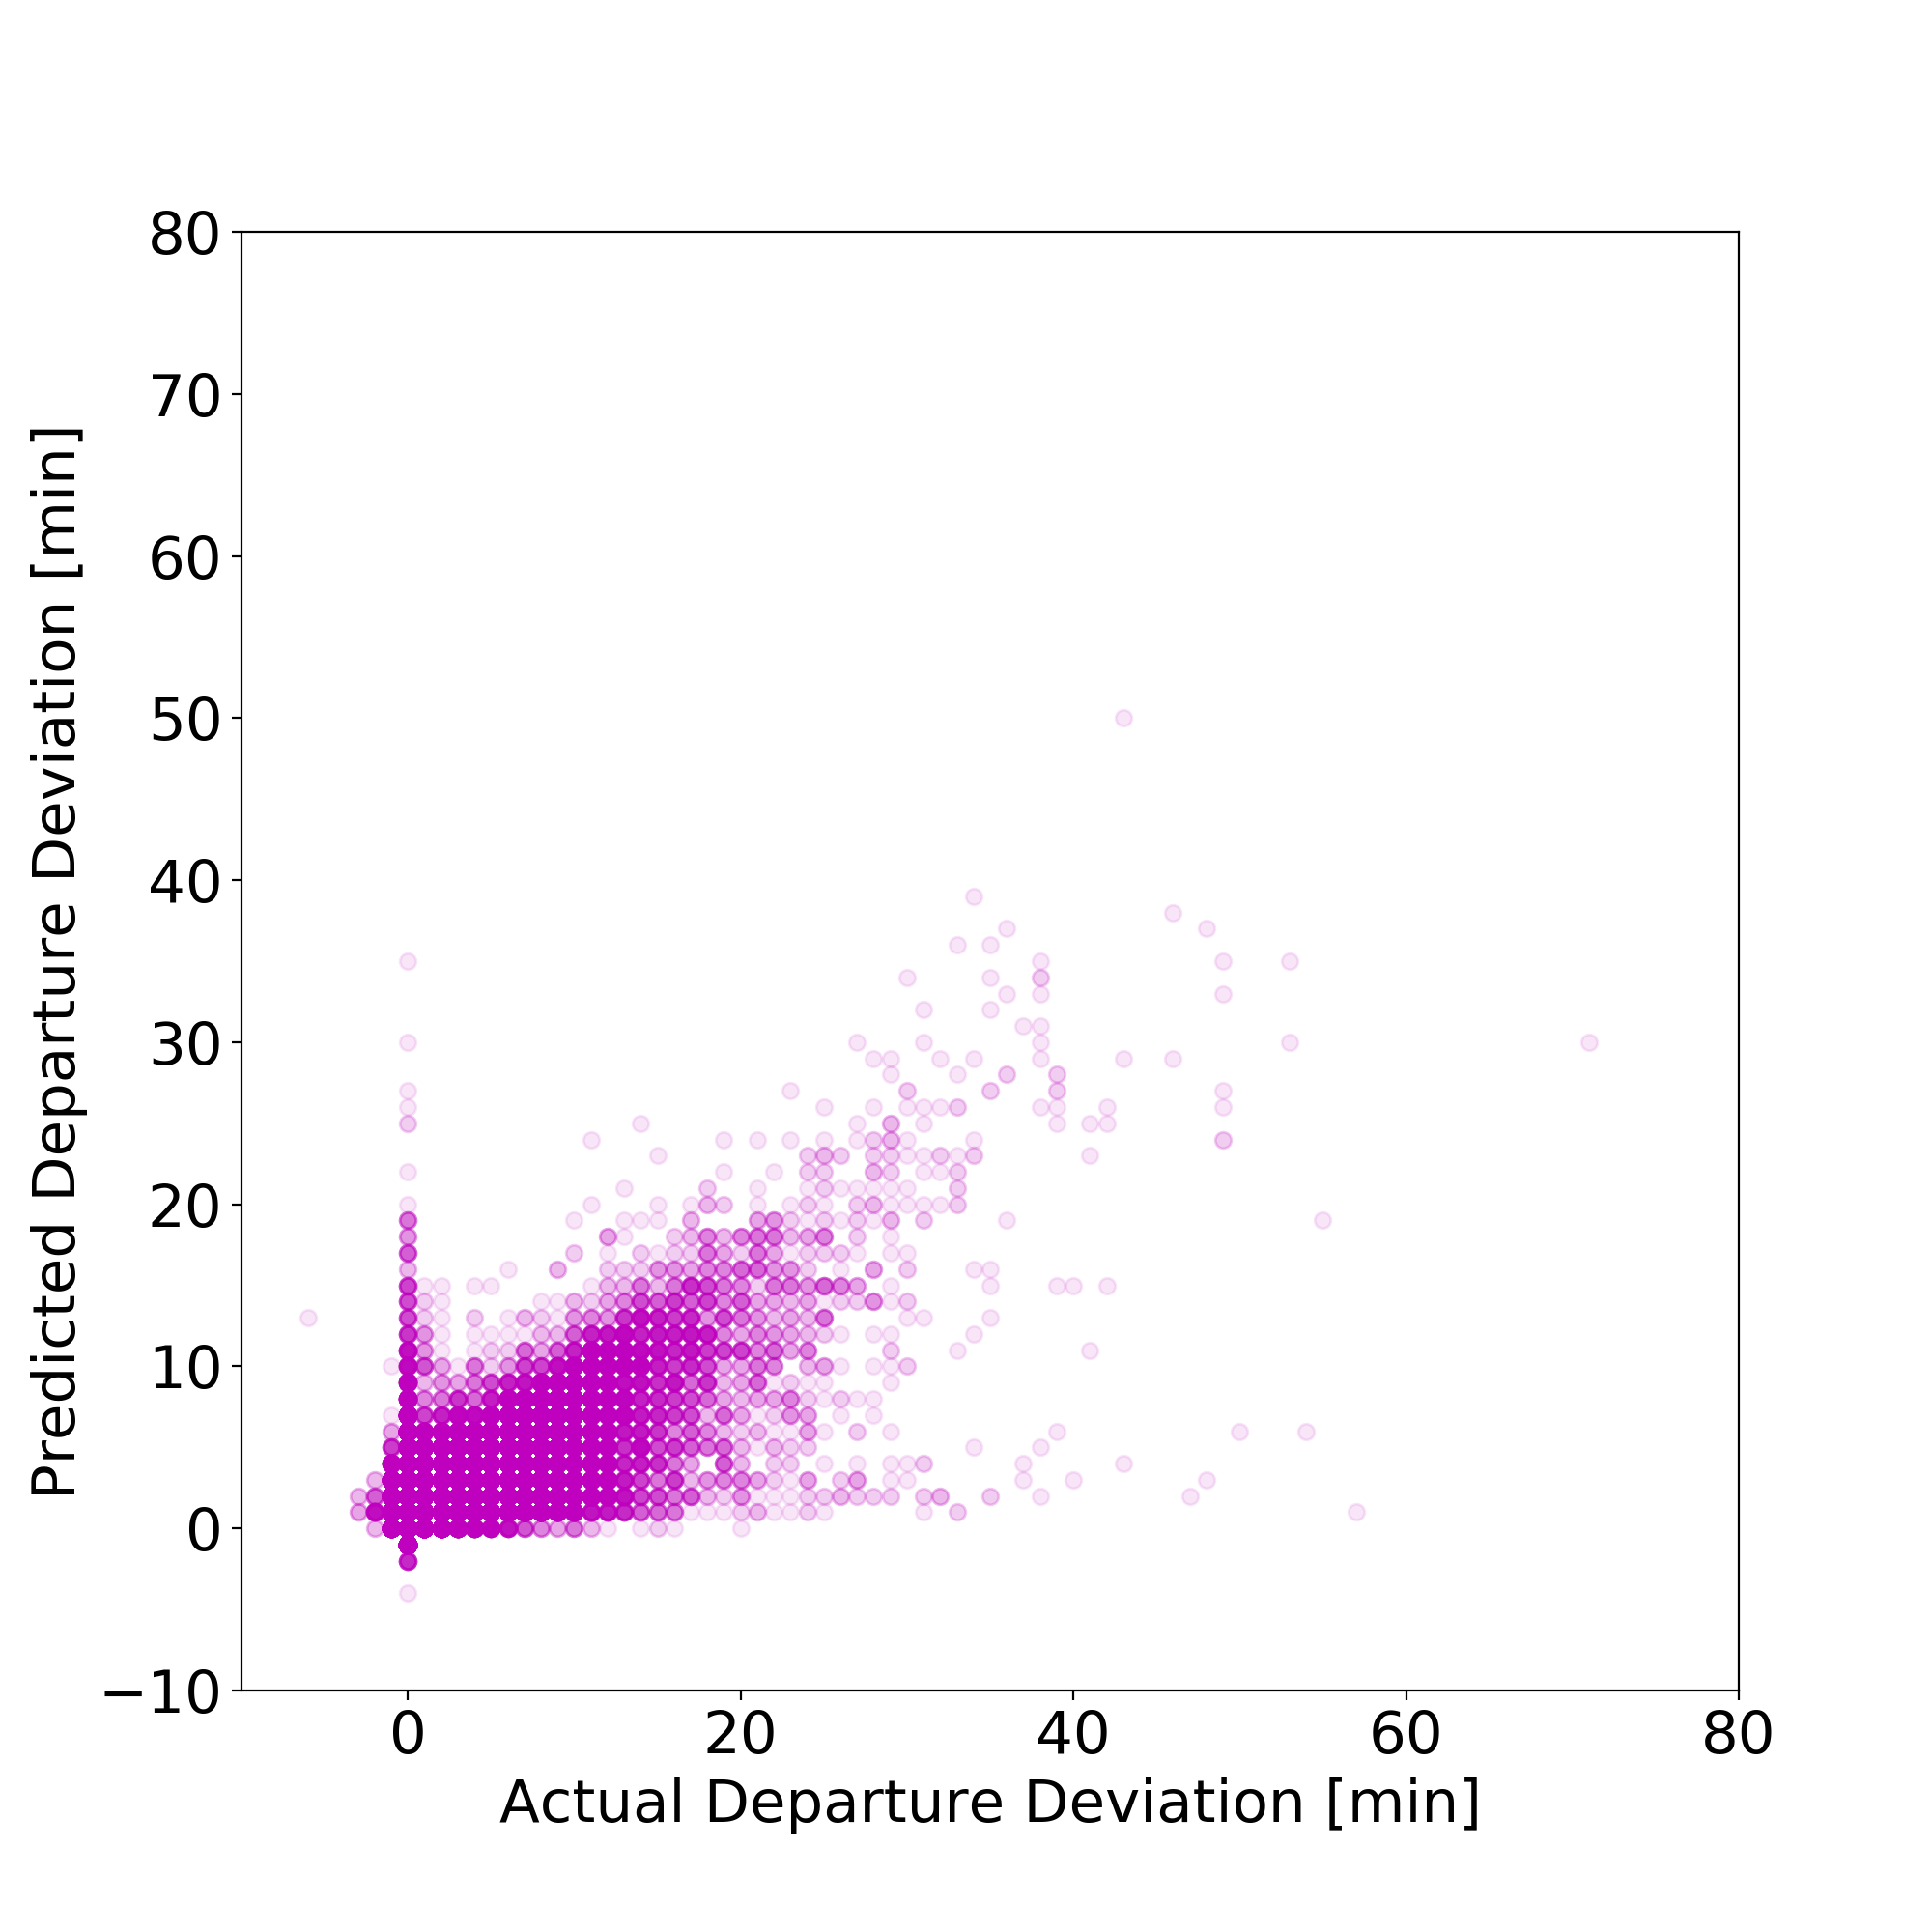
\includegraphics[width=0.5\textwidth]{Images/DNN_plot/4_step/4_step_depature_deviation.png}\label{fig:4_step_depature_deviation}}
\subfloat[\tiny{4-Step XGBoost Deviation from Departure}]{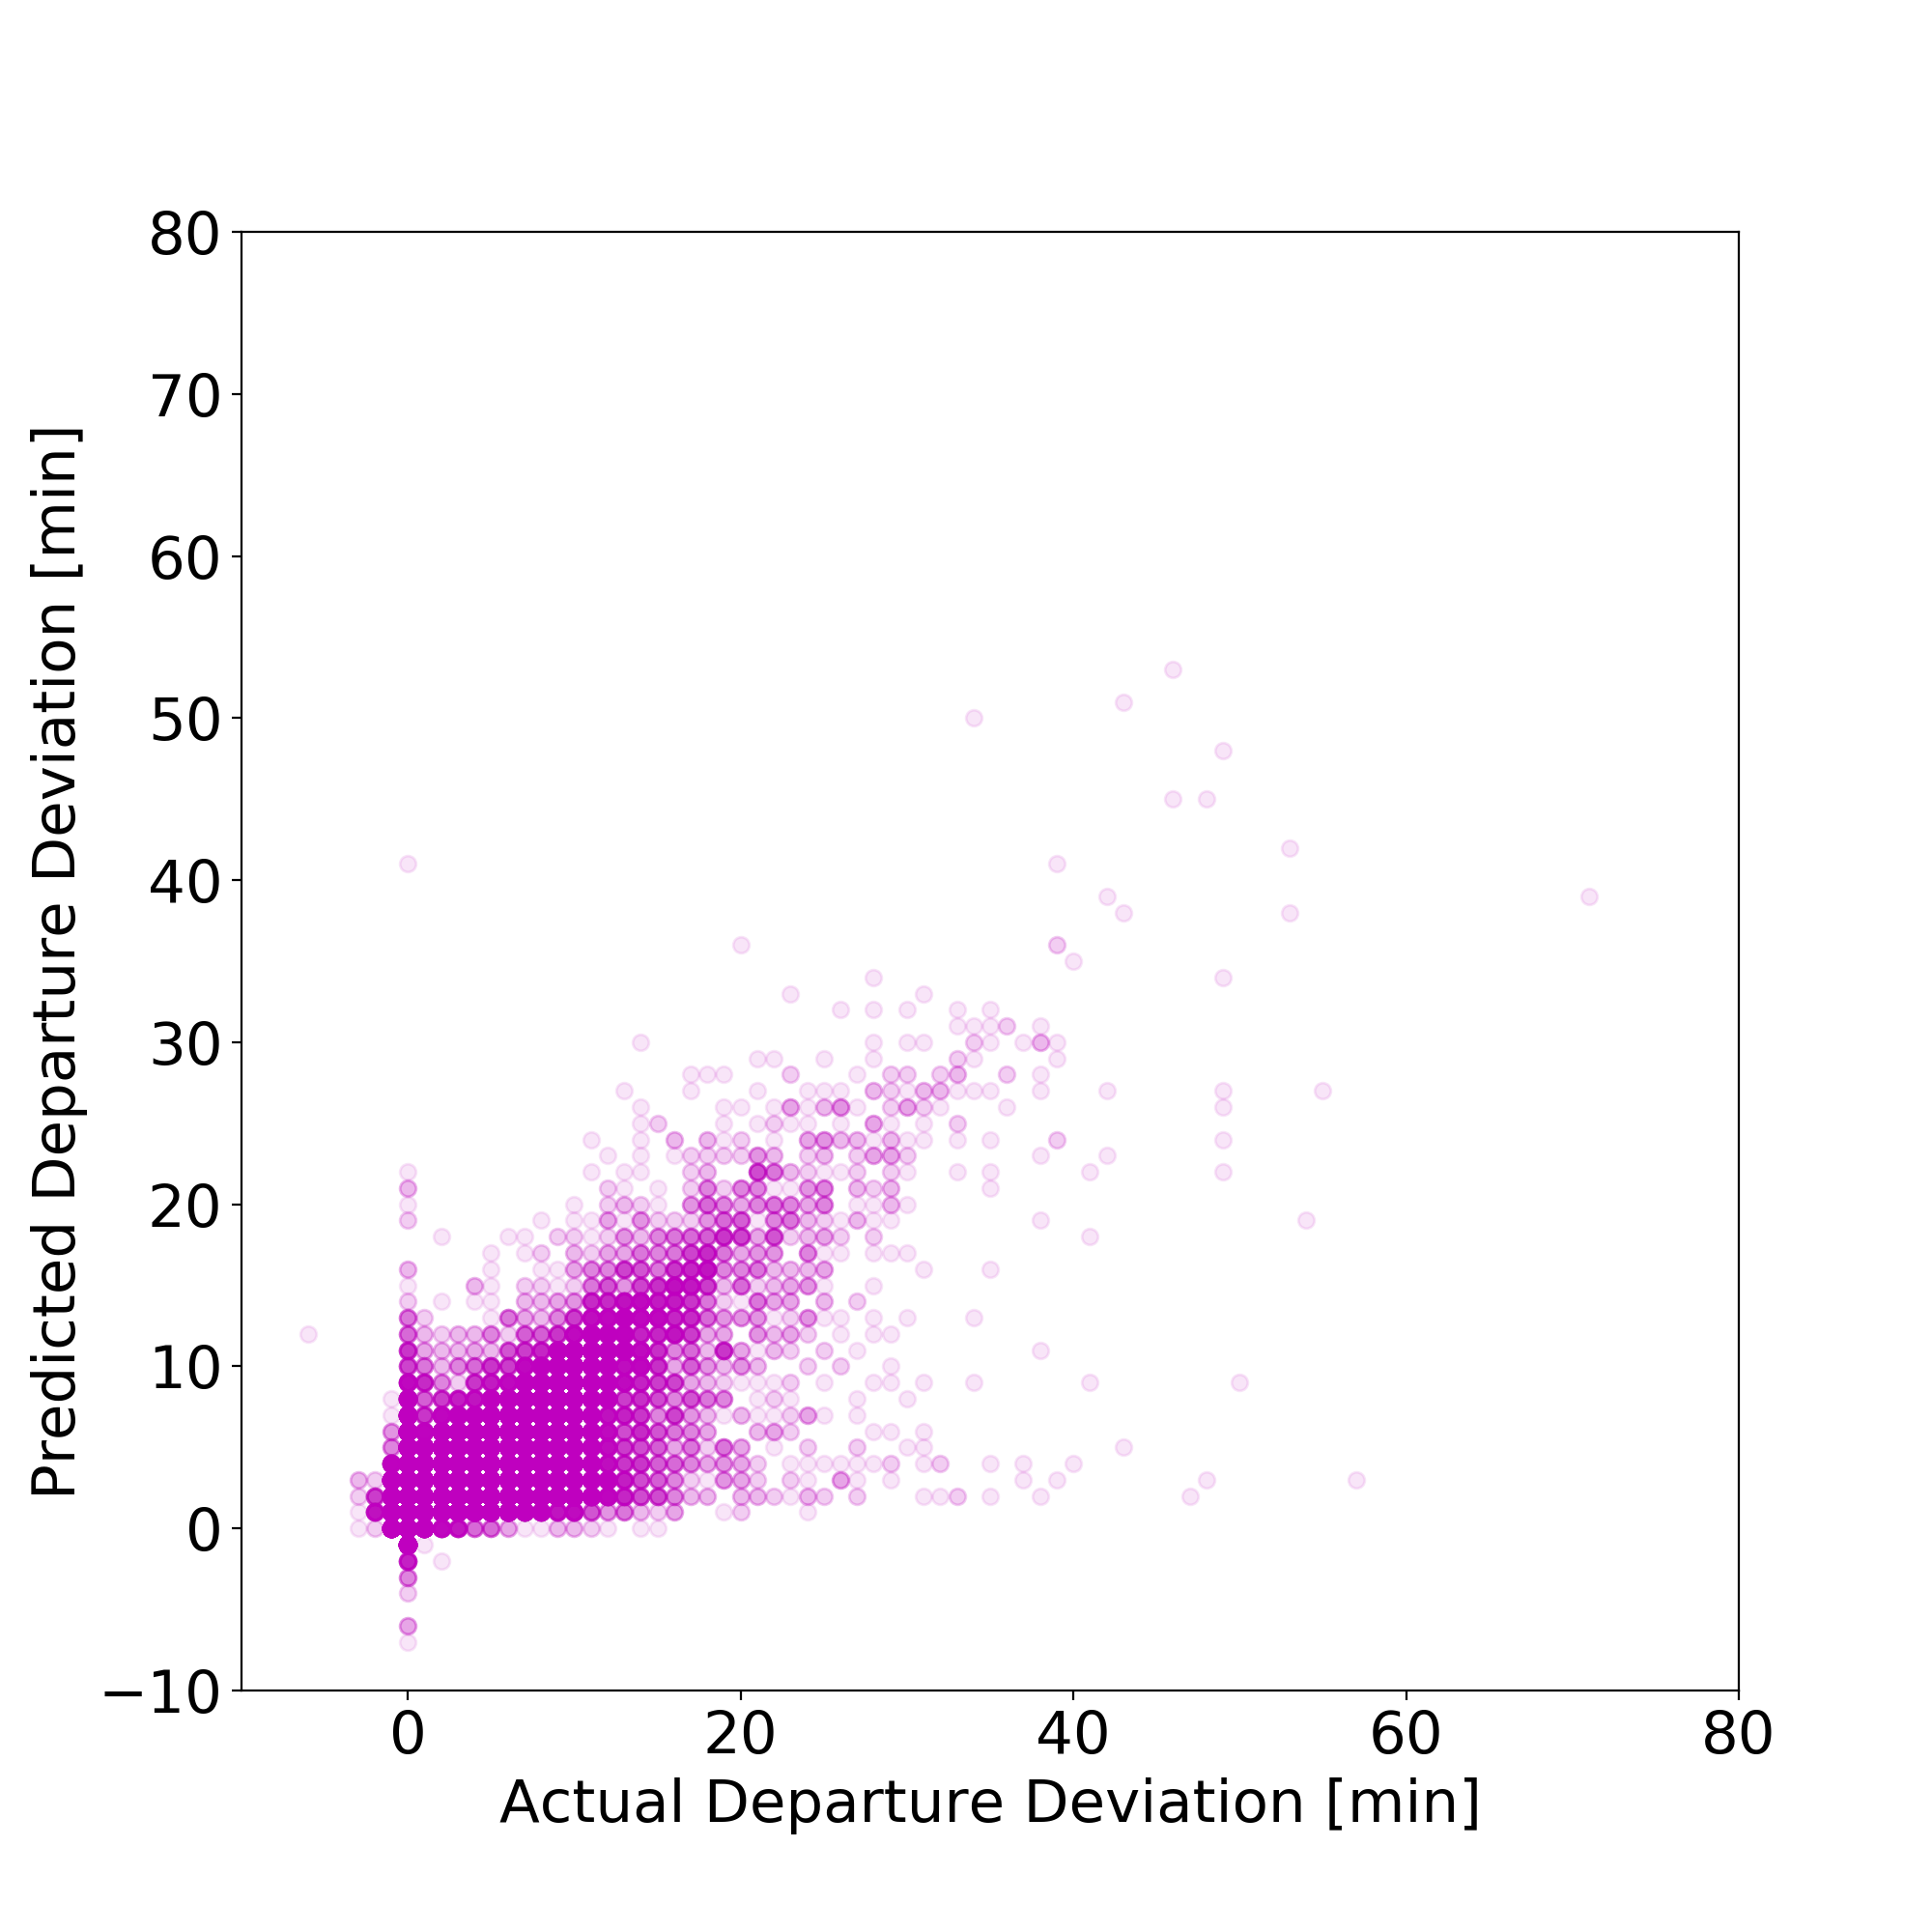
\includegraphics[width=0.5\textwidth]{Images/XGBoost_plot/4_step/4_step_depature_deviation.png}\label{fig:4_step_depature_deviation}}
\end{figure}
\begin{figure}[H]
\centering
\subfloat[\tiny{4-Step DNN Travel Time}]{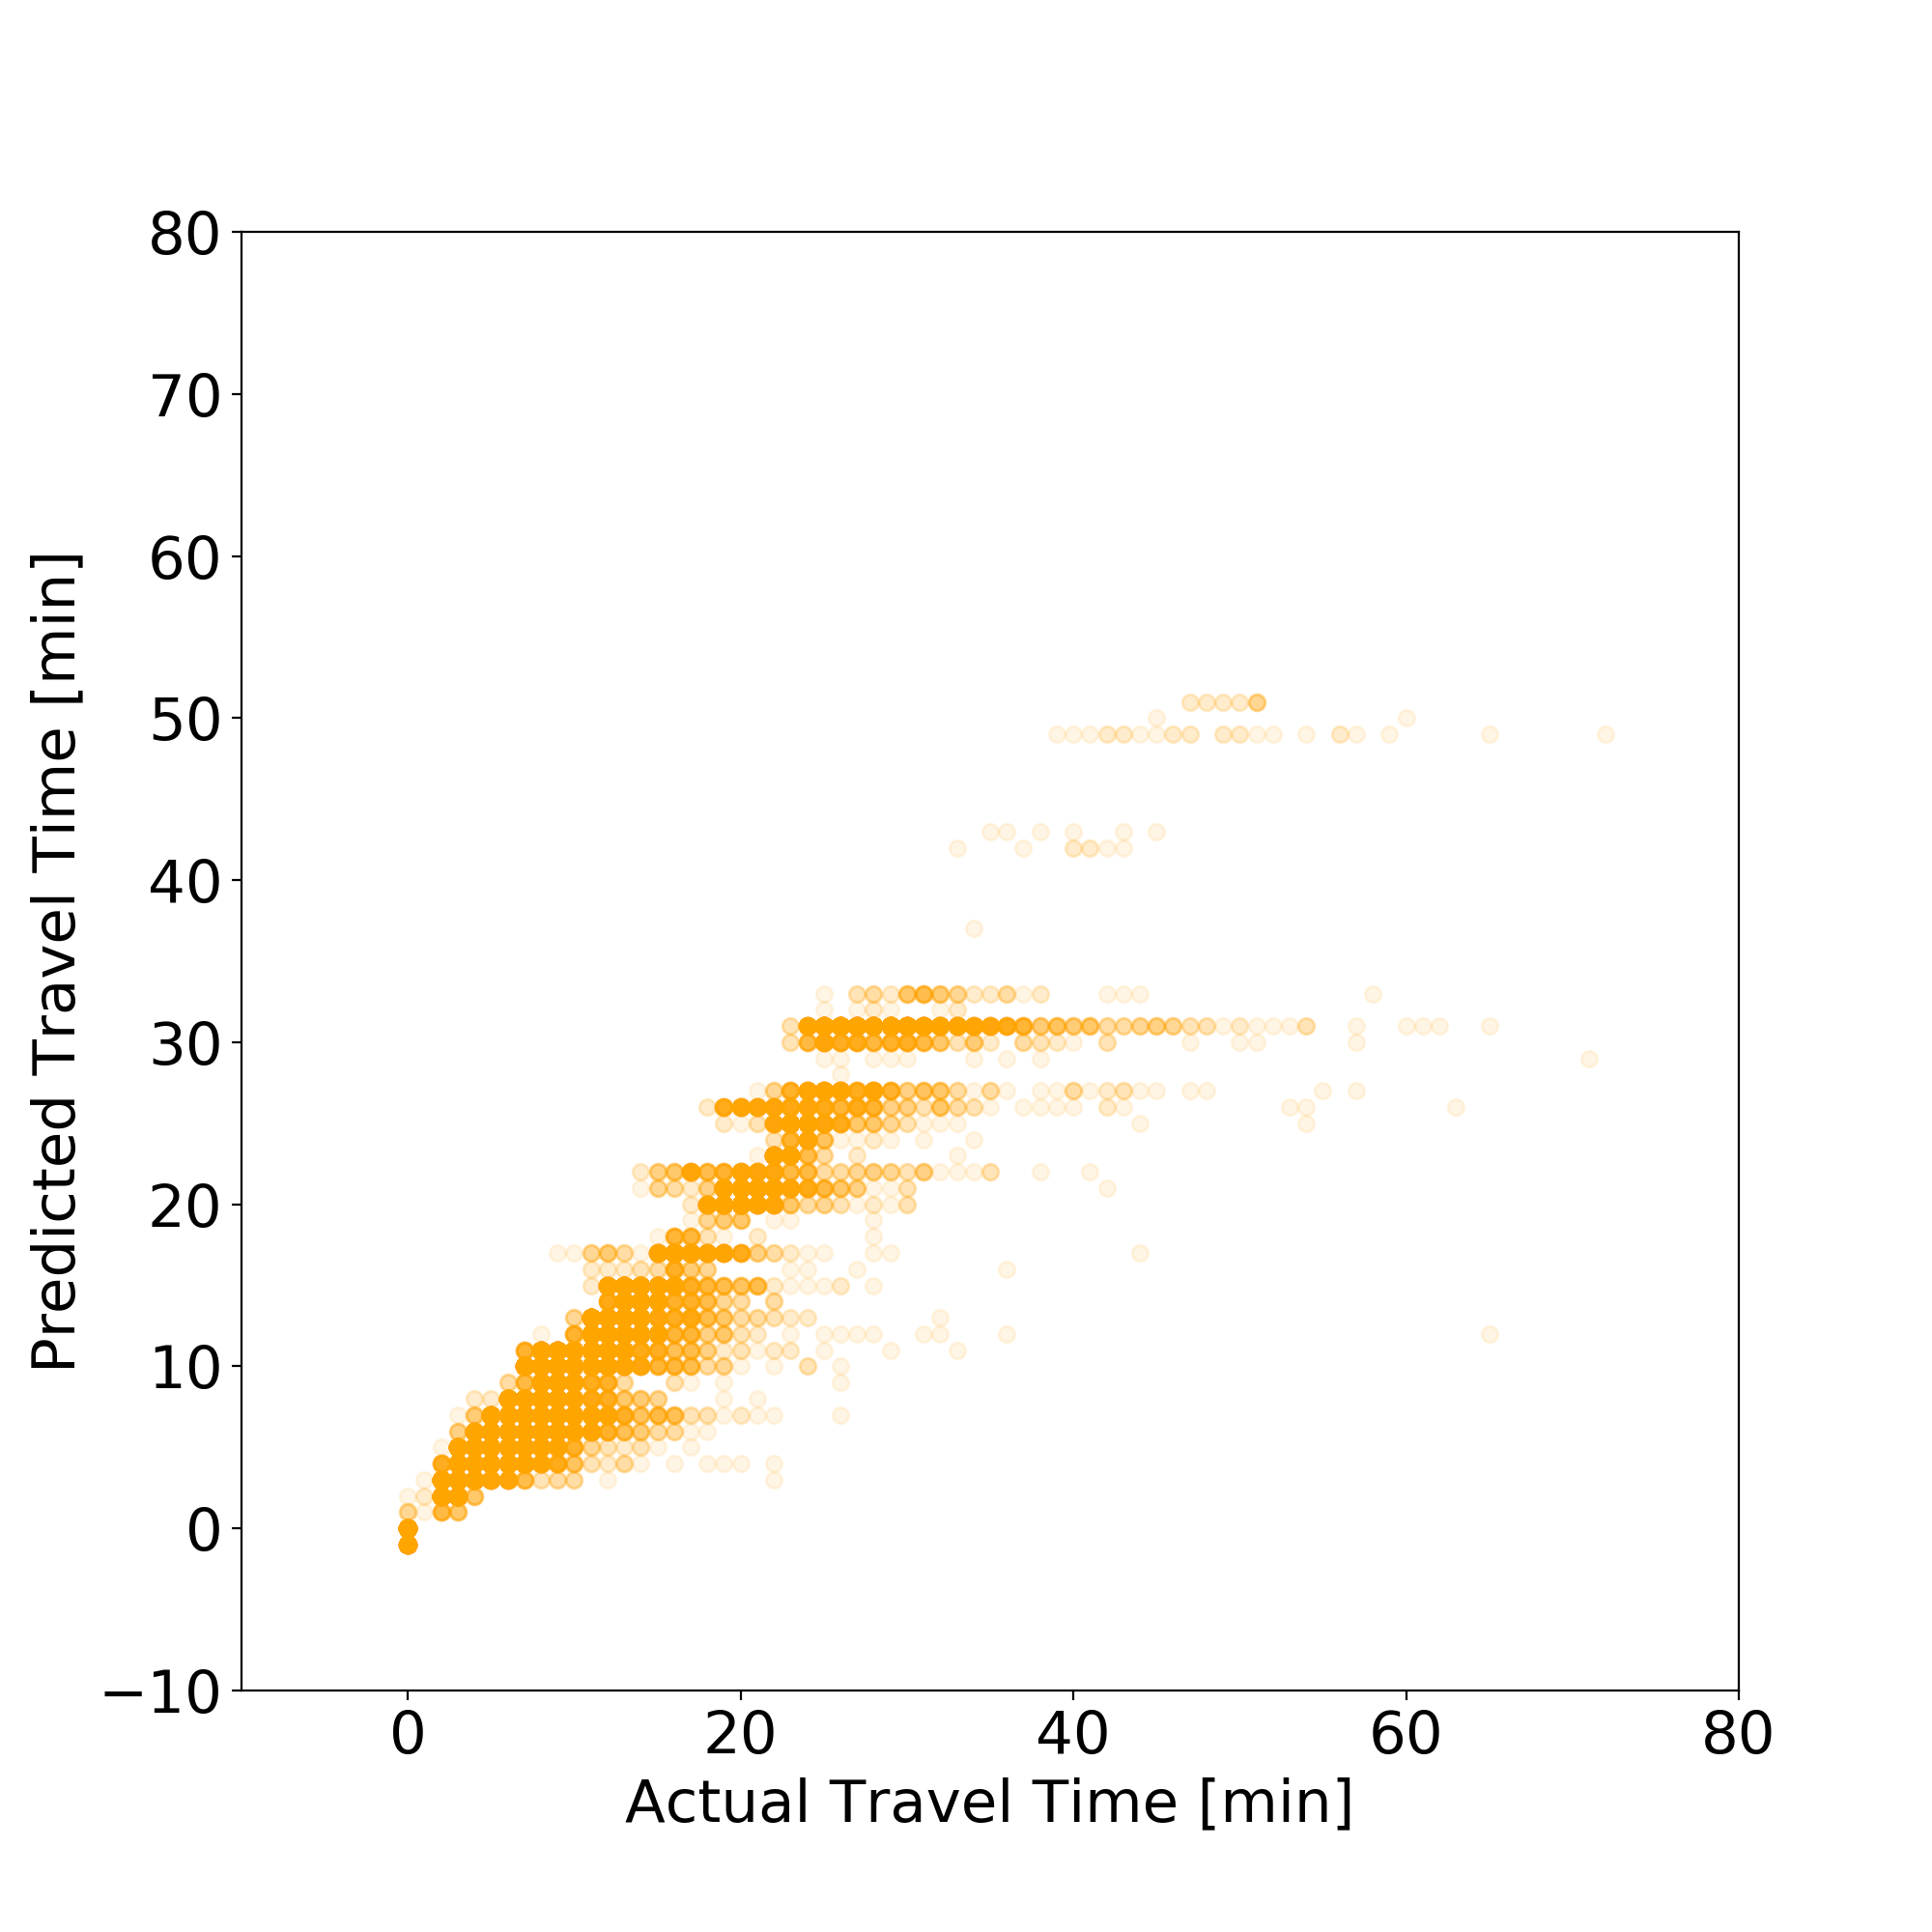
\includegraphics[width=0.5\textwidth]{Images/DNN_plot/4_step/4_step_travel_time.png}\label{fig:4_step_travel_time}}
\subfloat[\tiny{4-Step XGBoost Travel Time}]{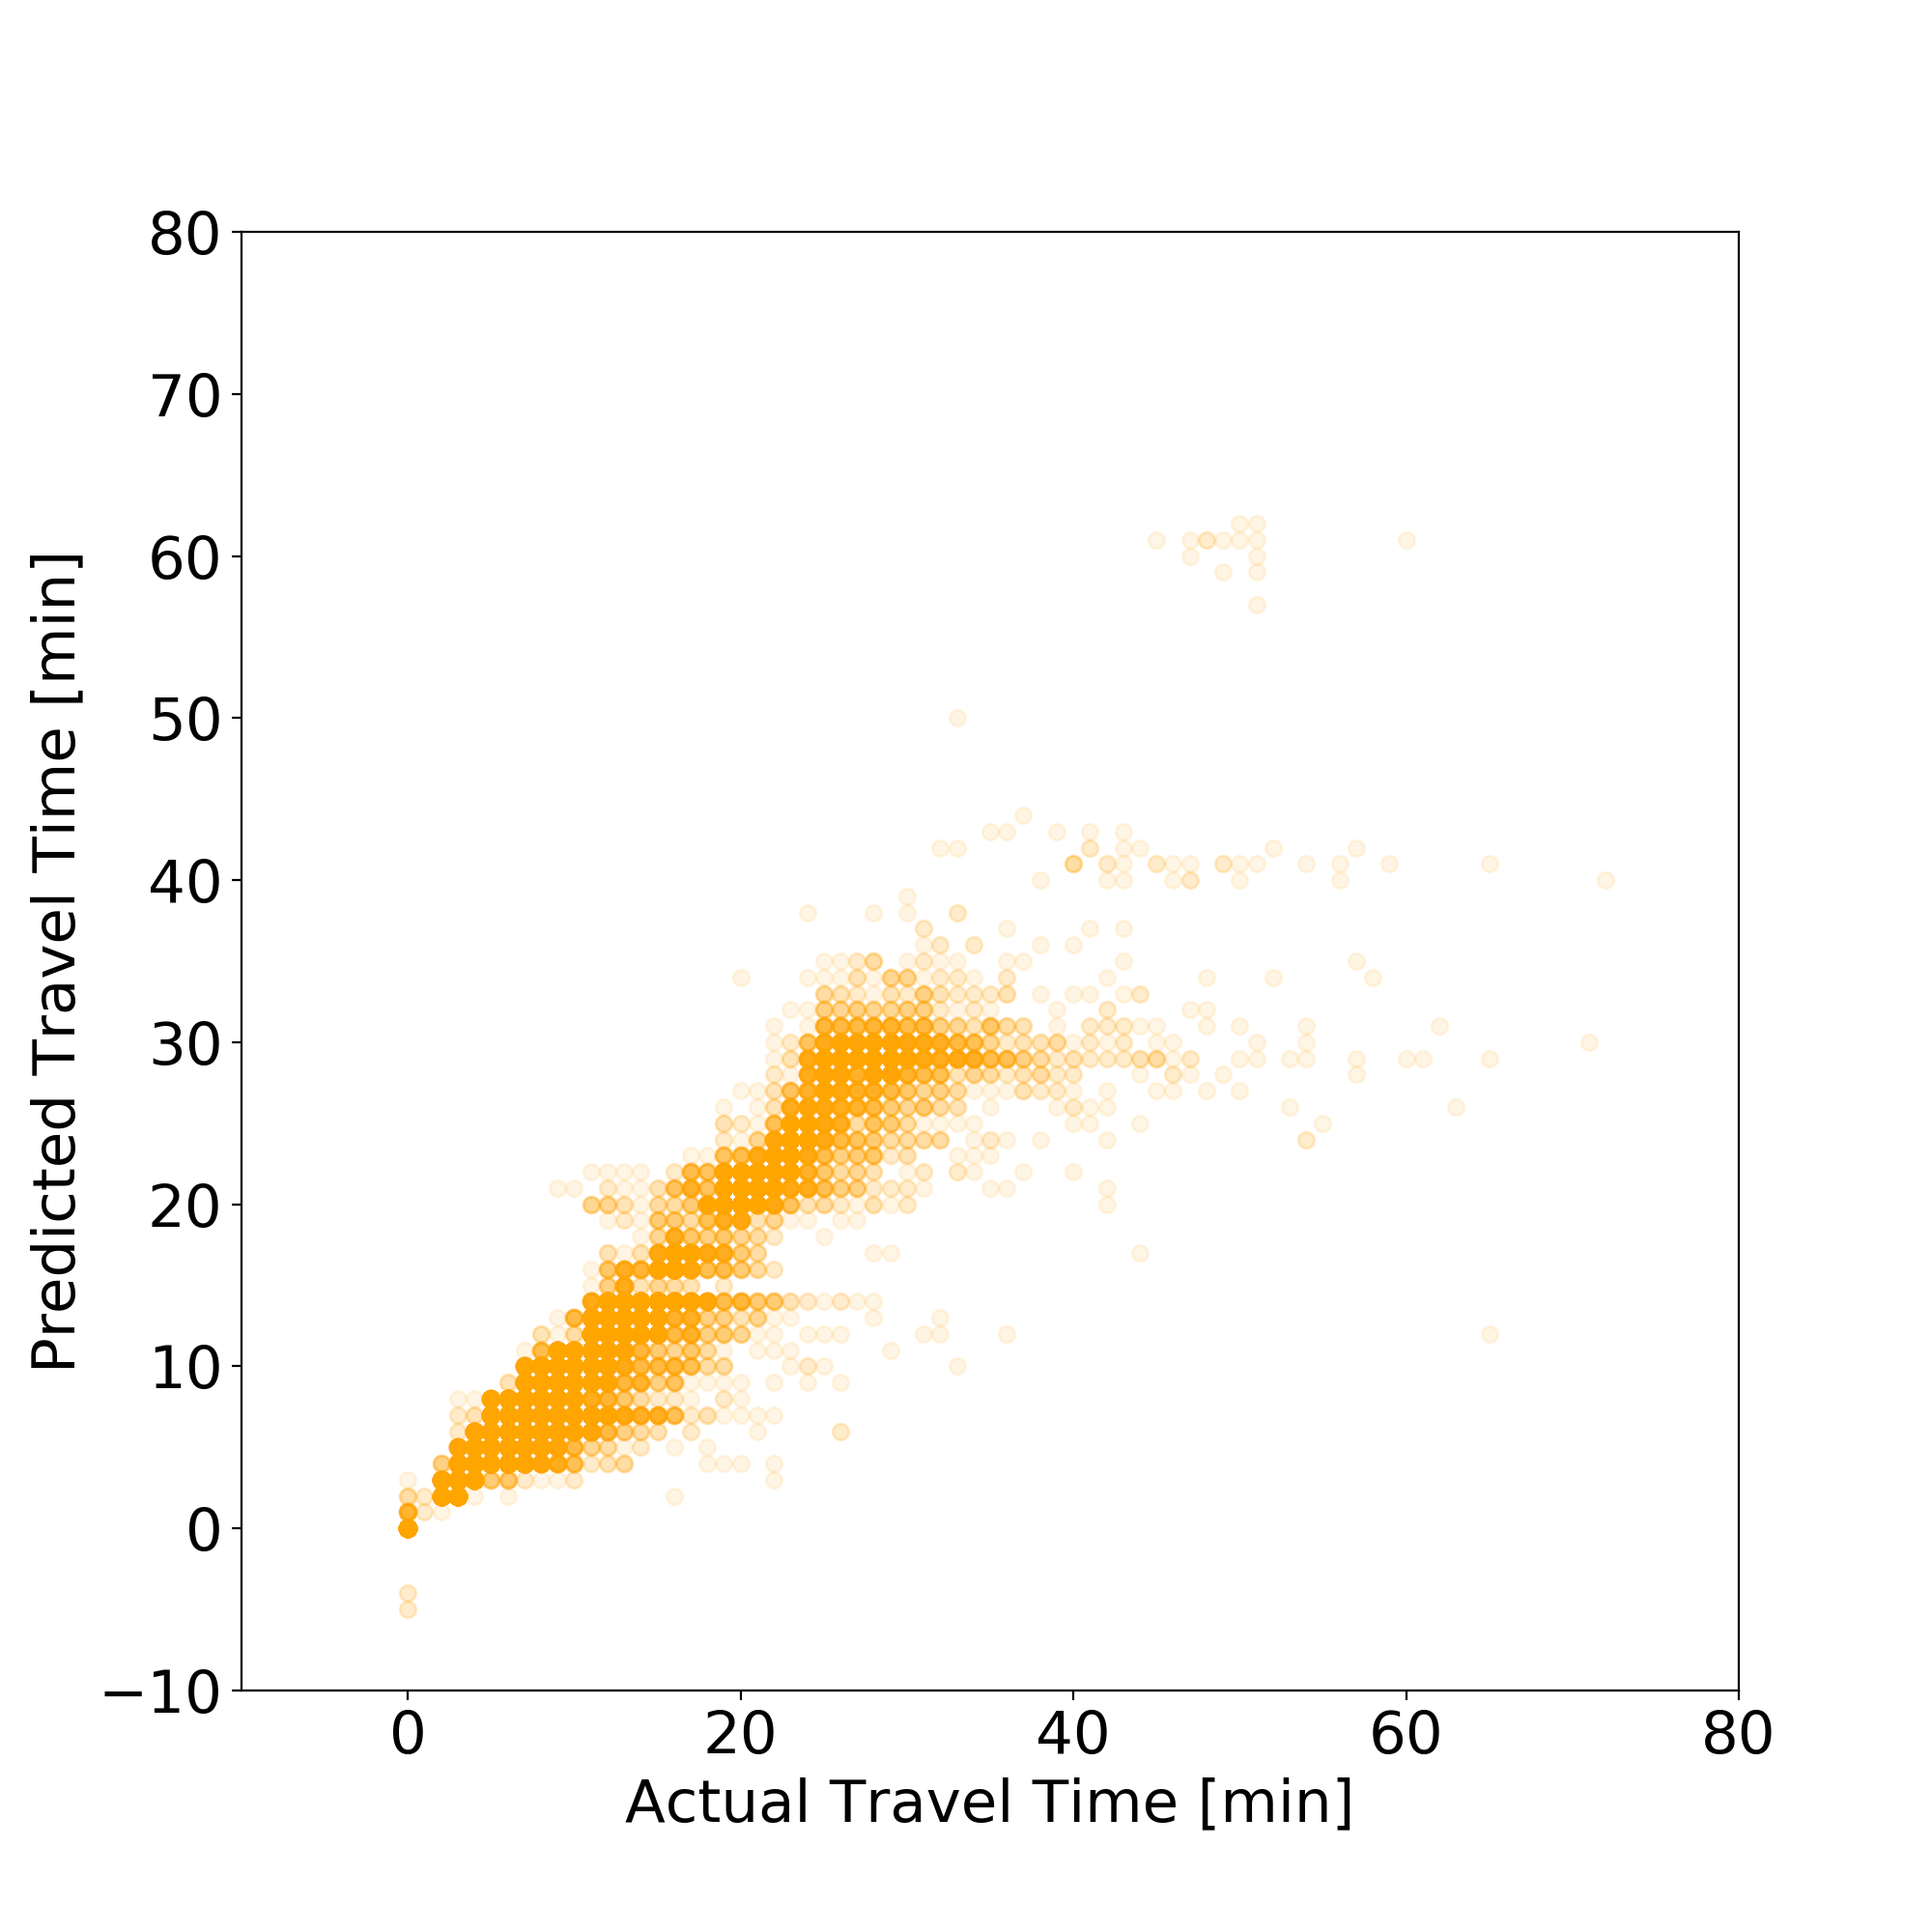
\includegraphics[width=0.5\textwidth]{Images/XGBoost_plot/4_step/4_step_travel_time.png}\label{fig:4_step_travel_time}}
\end{figure}
\begin{figure}[H]
\centering
\subfloat[\tiny{4-Step DNN Dwell Time}]{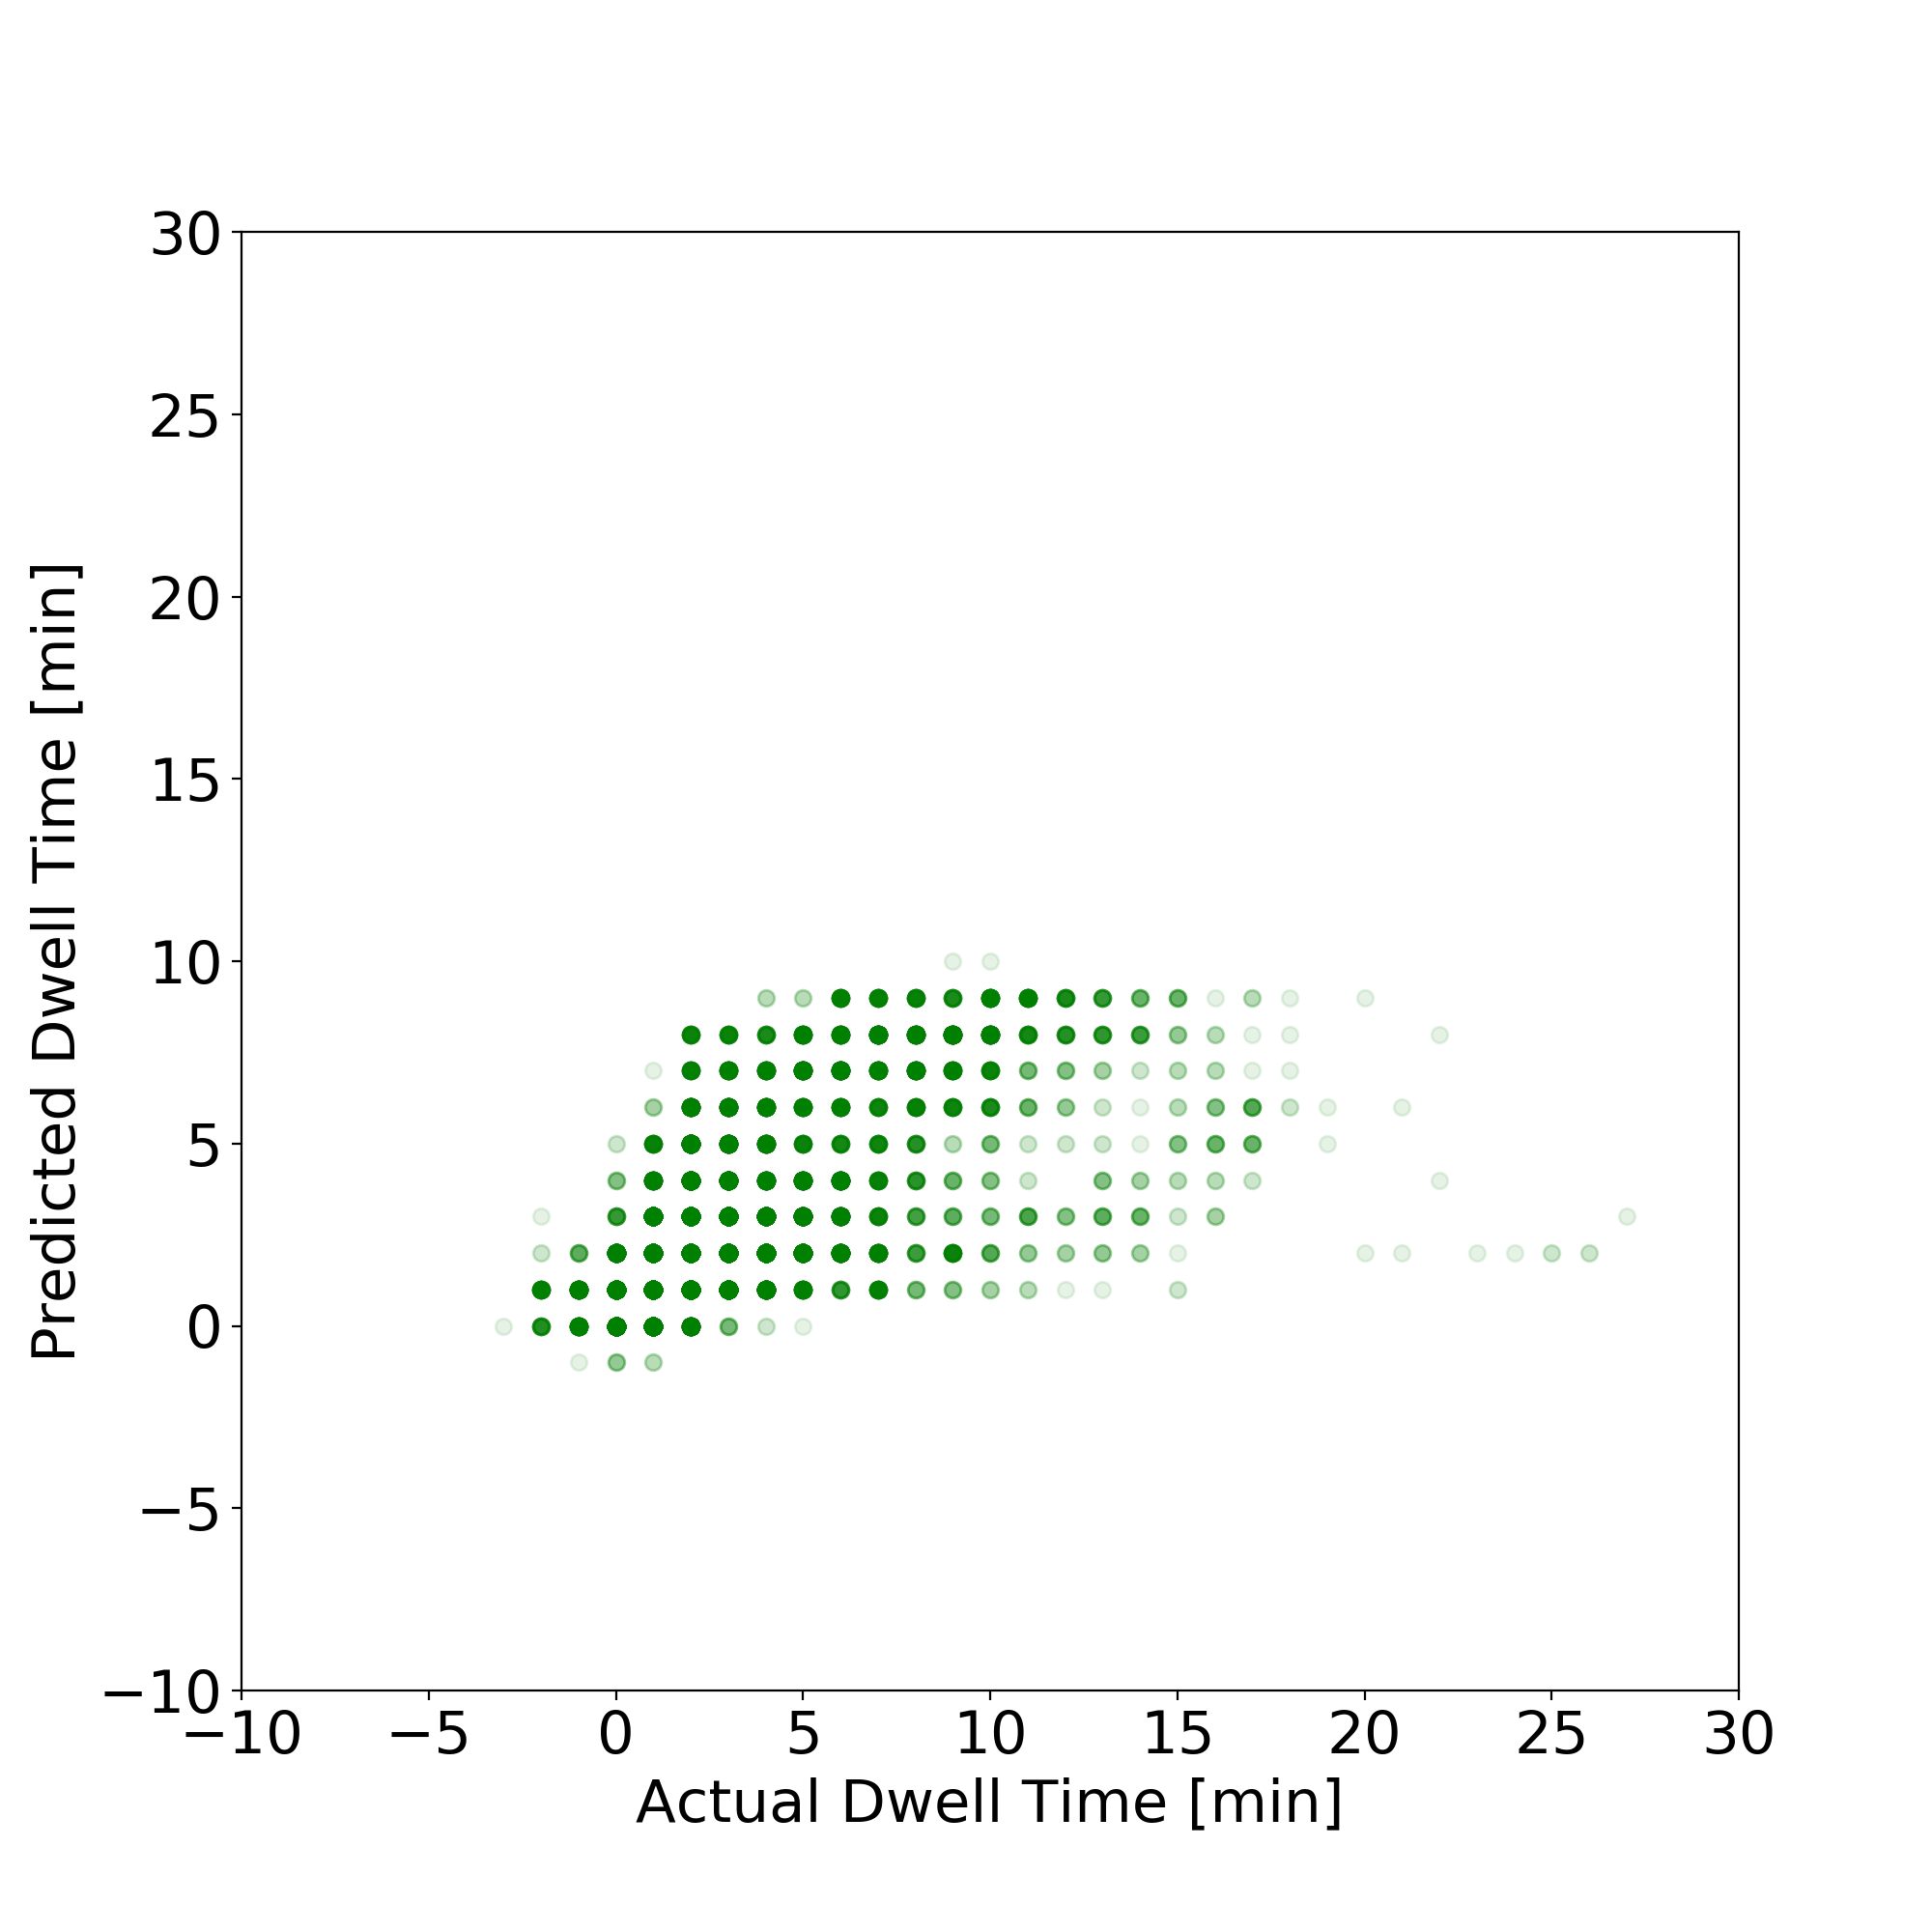
\includegraphics[width=0.5\textwidth]{Images/DNN_plot/4_step/4_step_dwell_time.png}\label{fig:4_step_dwell_time}}
\subfloat[\tiny{4-Step XGBoost Dwell Time}]{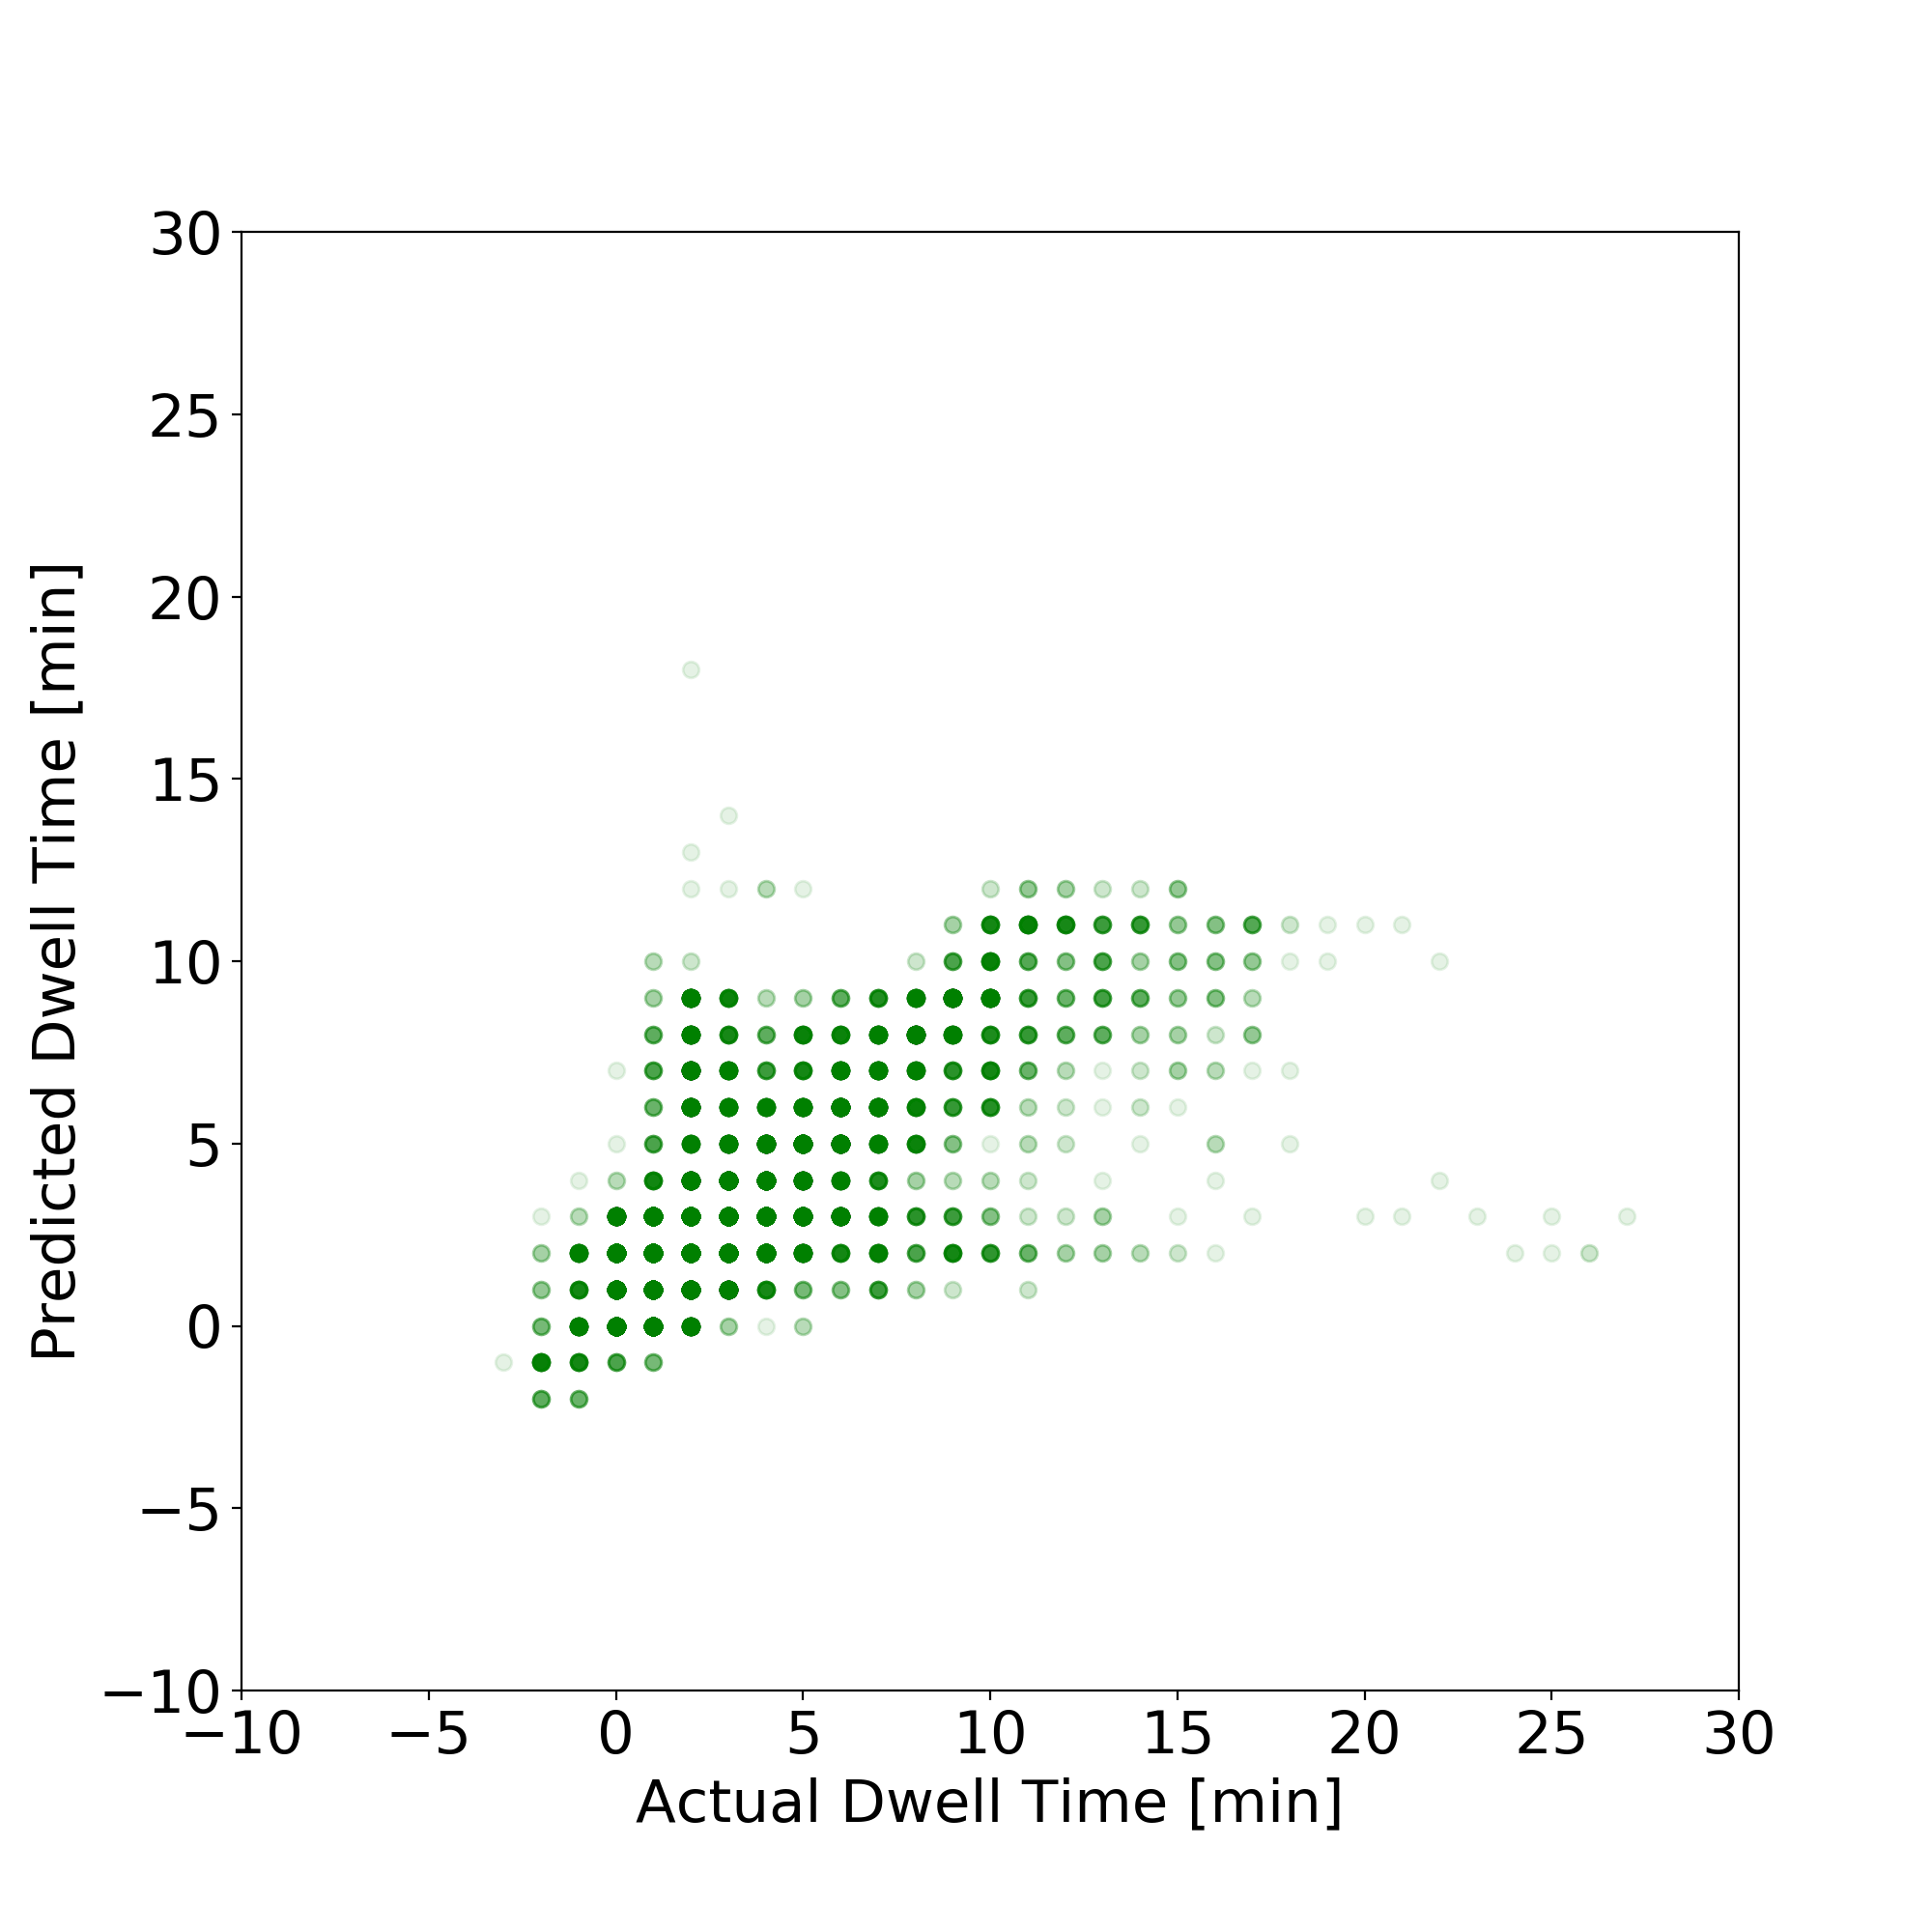
\includegraphics[width=0.5\textwidth]{Images/XGBoost_plot/4_step/4_step_dwell_time.png}\label{fig:4_step_dwell_time}}
\end{figure}

\begin{figure}[H]
\centering
\subfloat[\tiny{5-Step DNN Deviation from Arrival}]{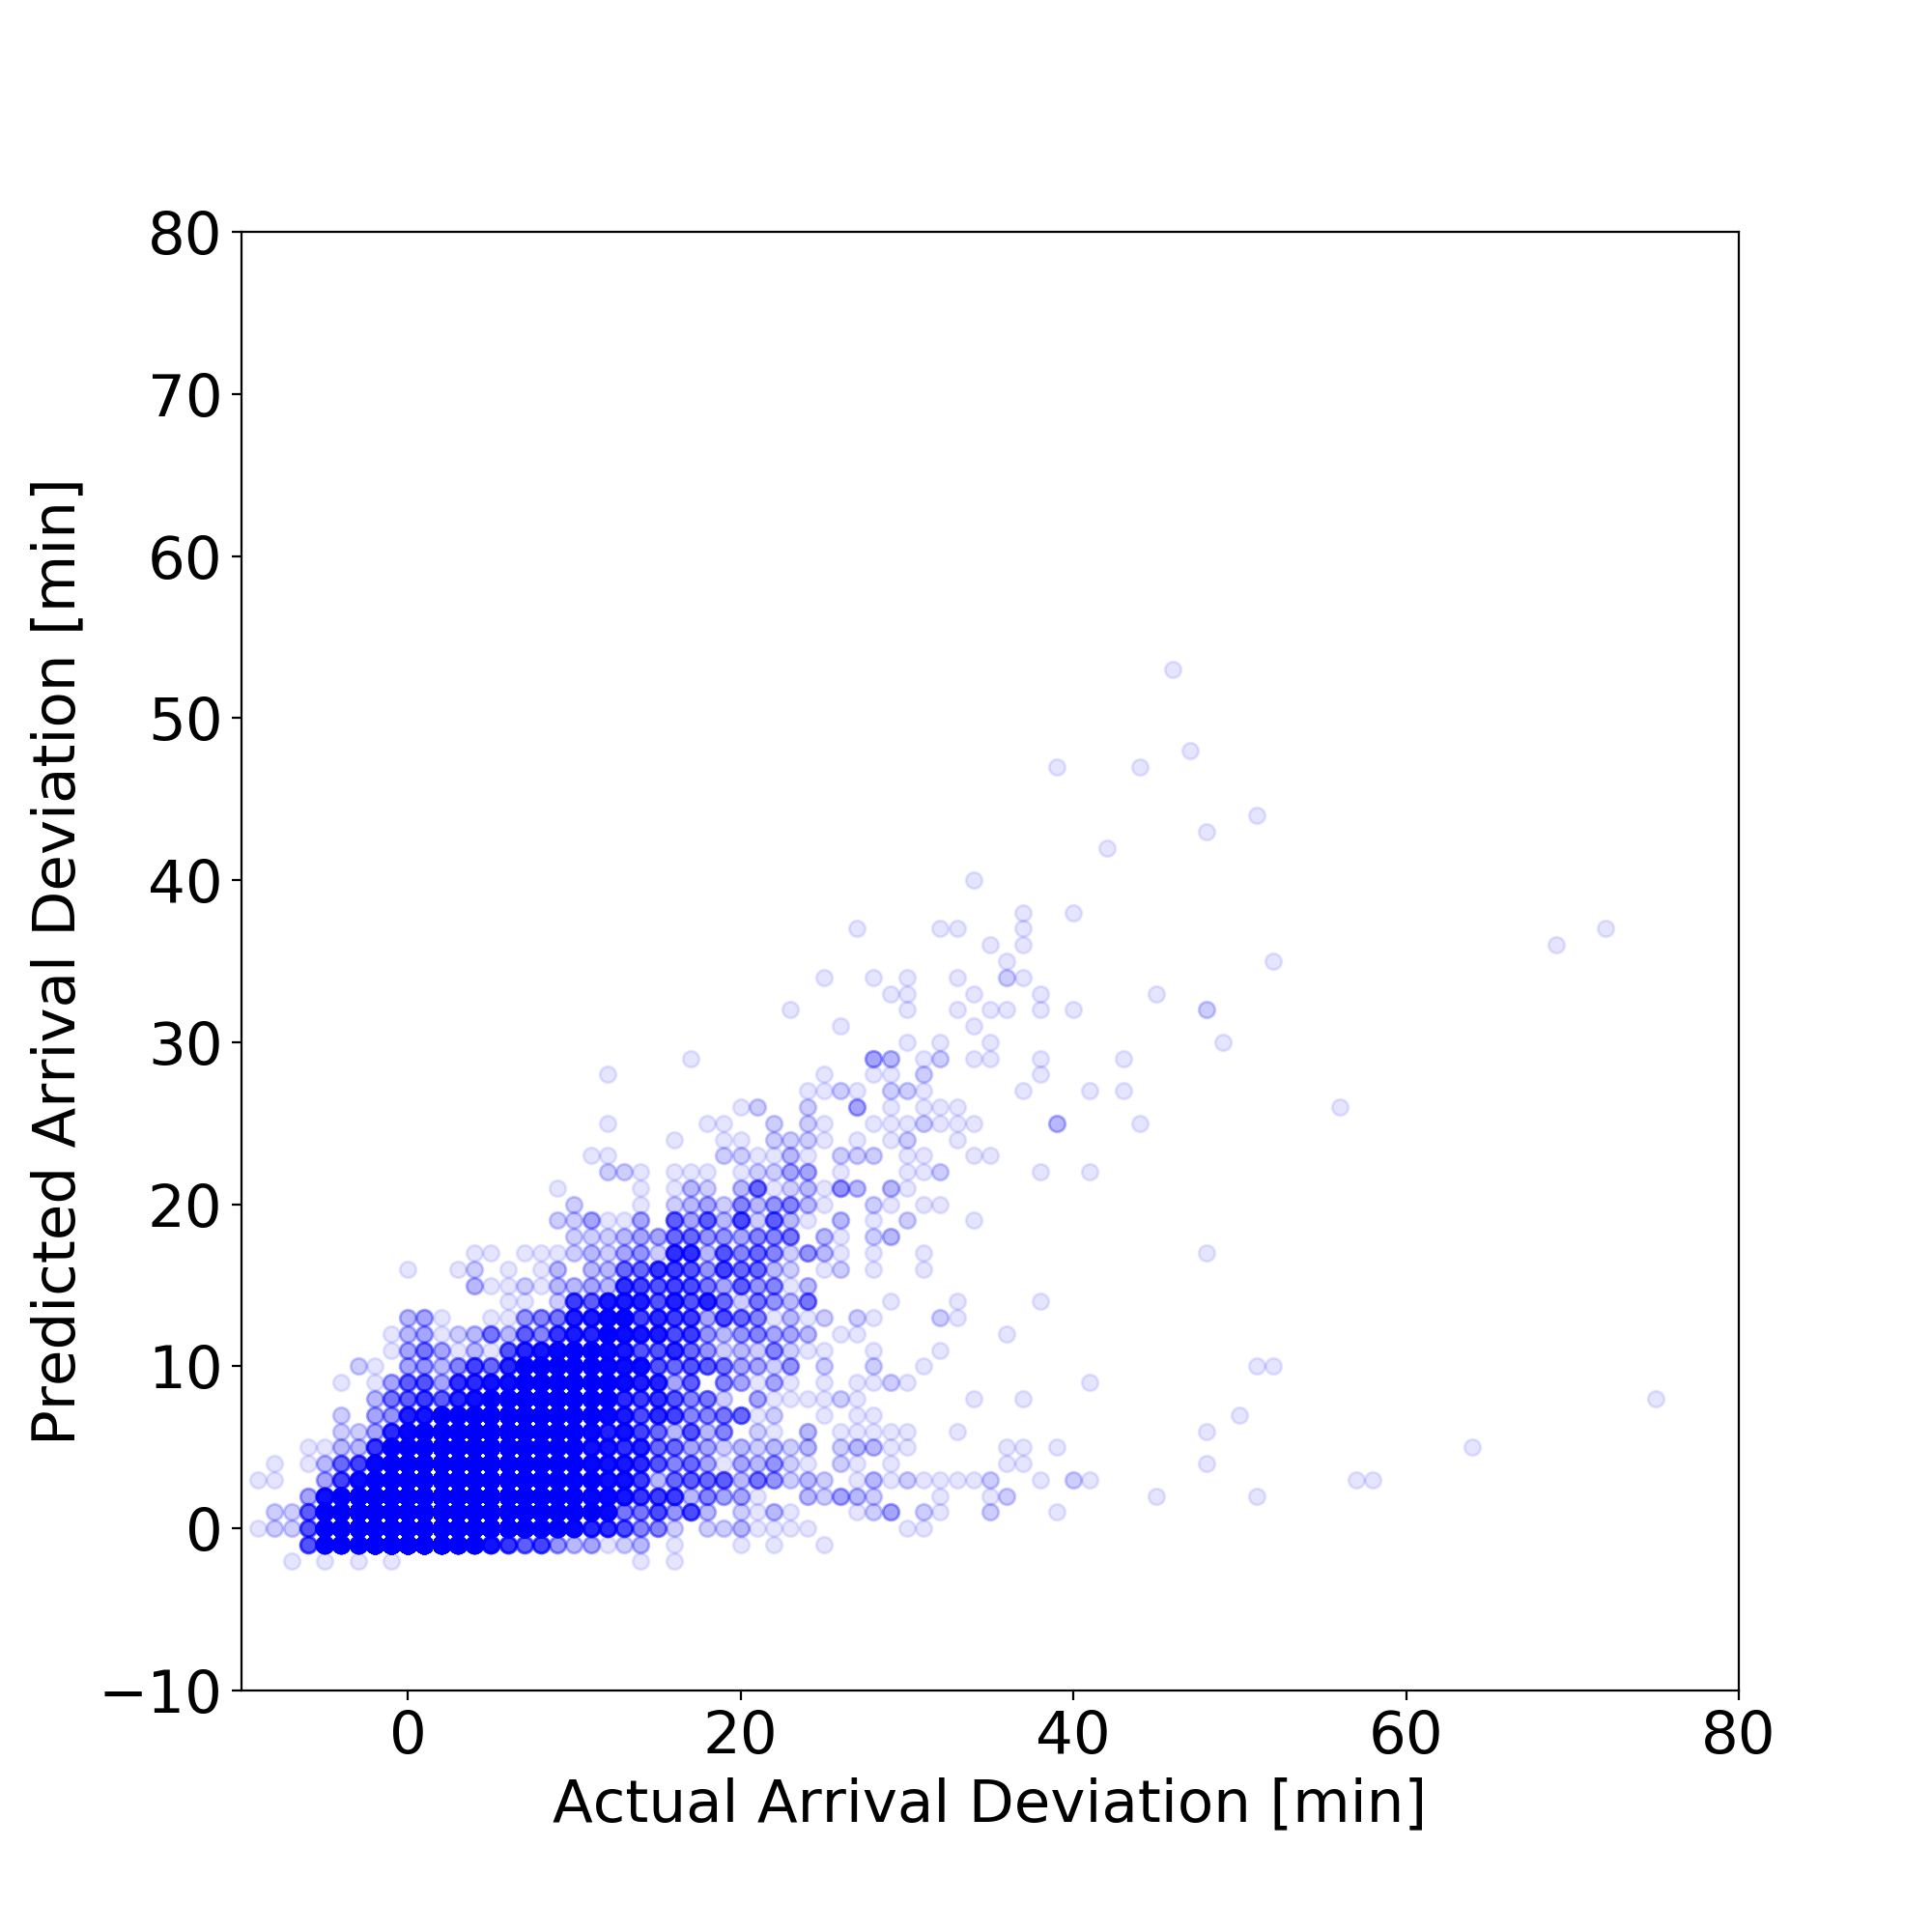
\includegraphics[width=0.5\textwidth]{Images/DNN_plot/5_step/5_step_arrival_deviation.png}\label{fig:5_step_arrival_deviation}}
\subfloat[\tiny{5-Step XGBoost Deviation from Arrival}]{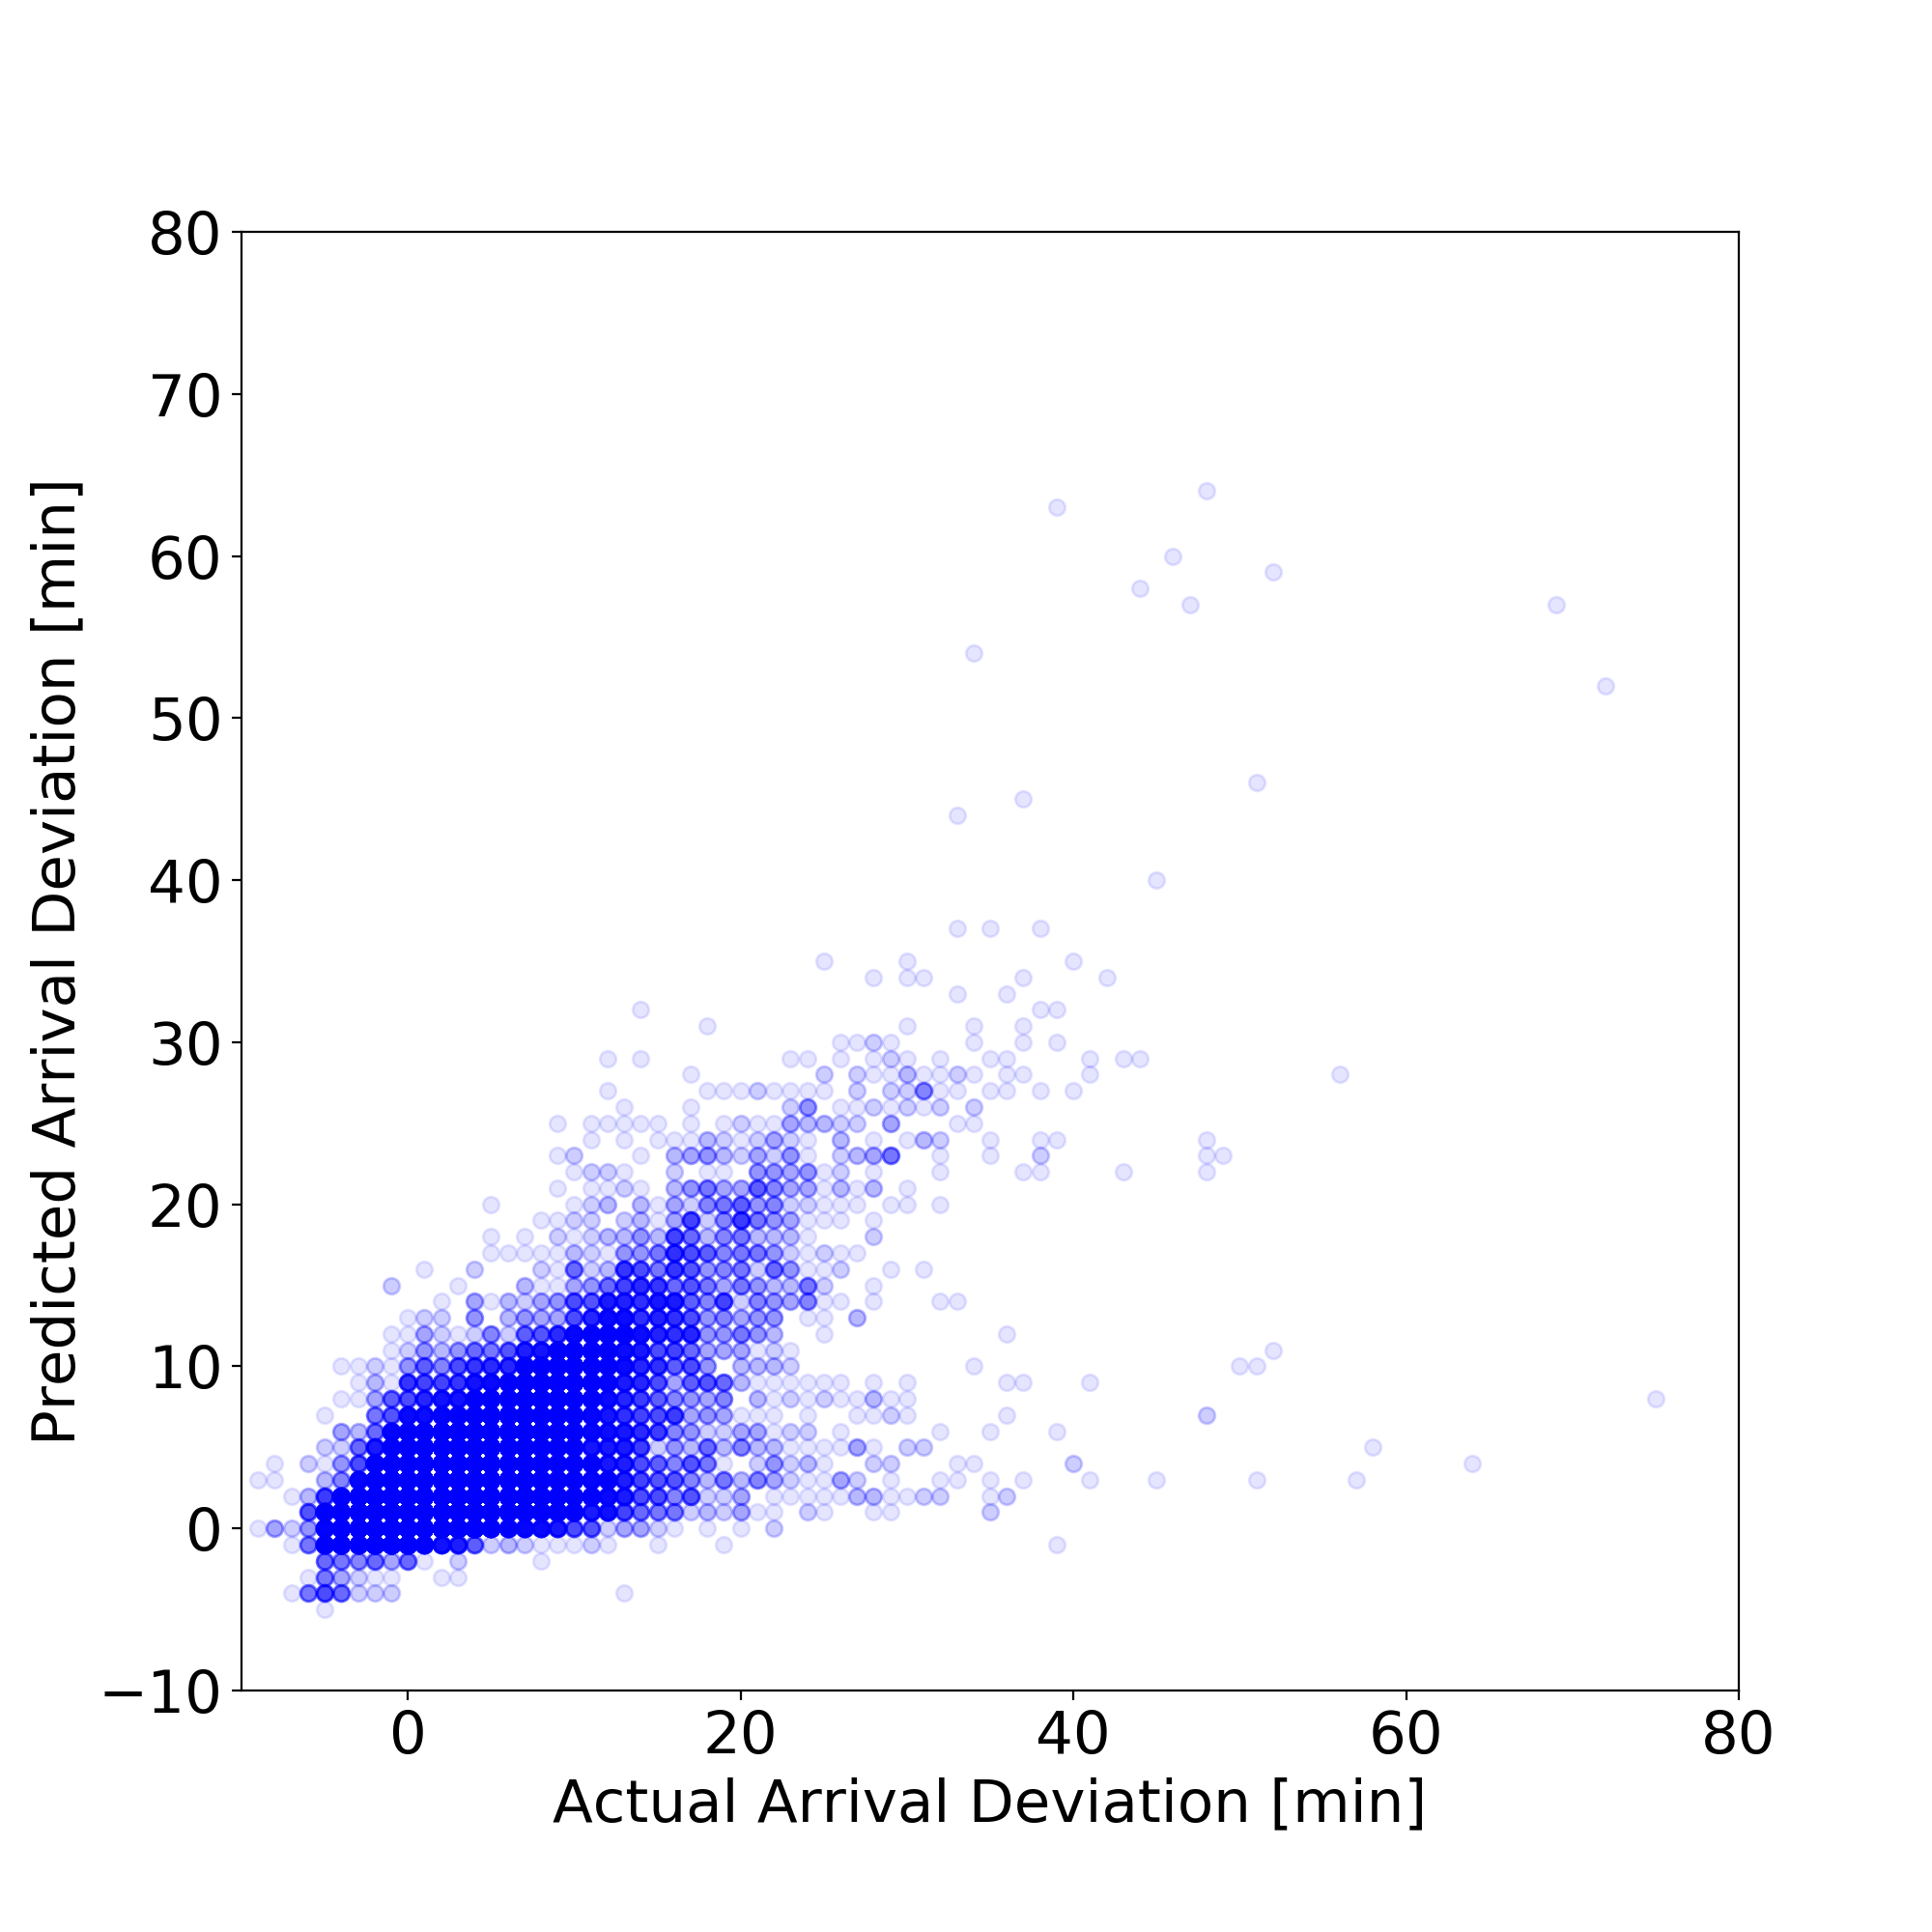
\includegraphics[width=0.5\textwidth]{Images/XGBoost_plot/5_step/5_step_arrival_deviation.png}\label{fig:5_step_arrival_deviation}}
\end{figure}
\begin{figure}[H]
\centering
\subfloat[\tiny{5-Step DNN Deviation from Departure}]{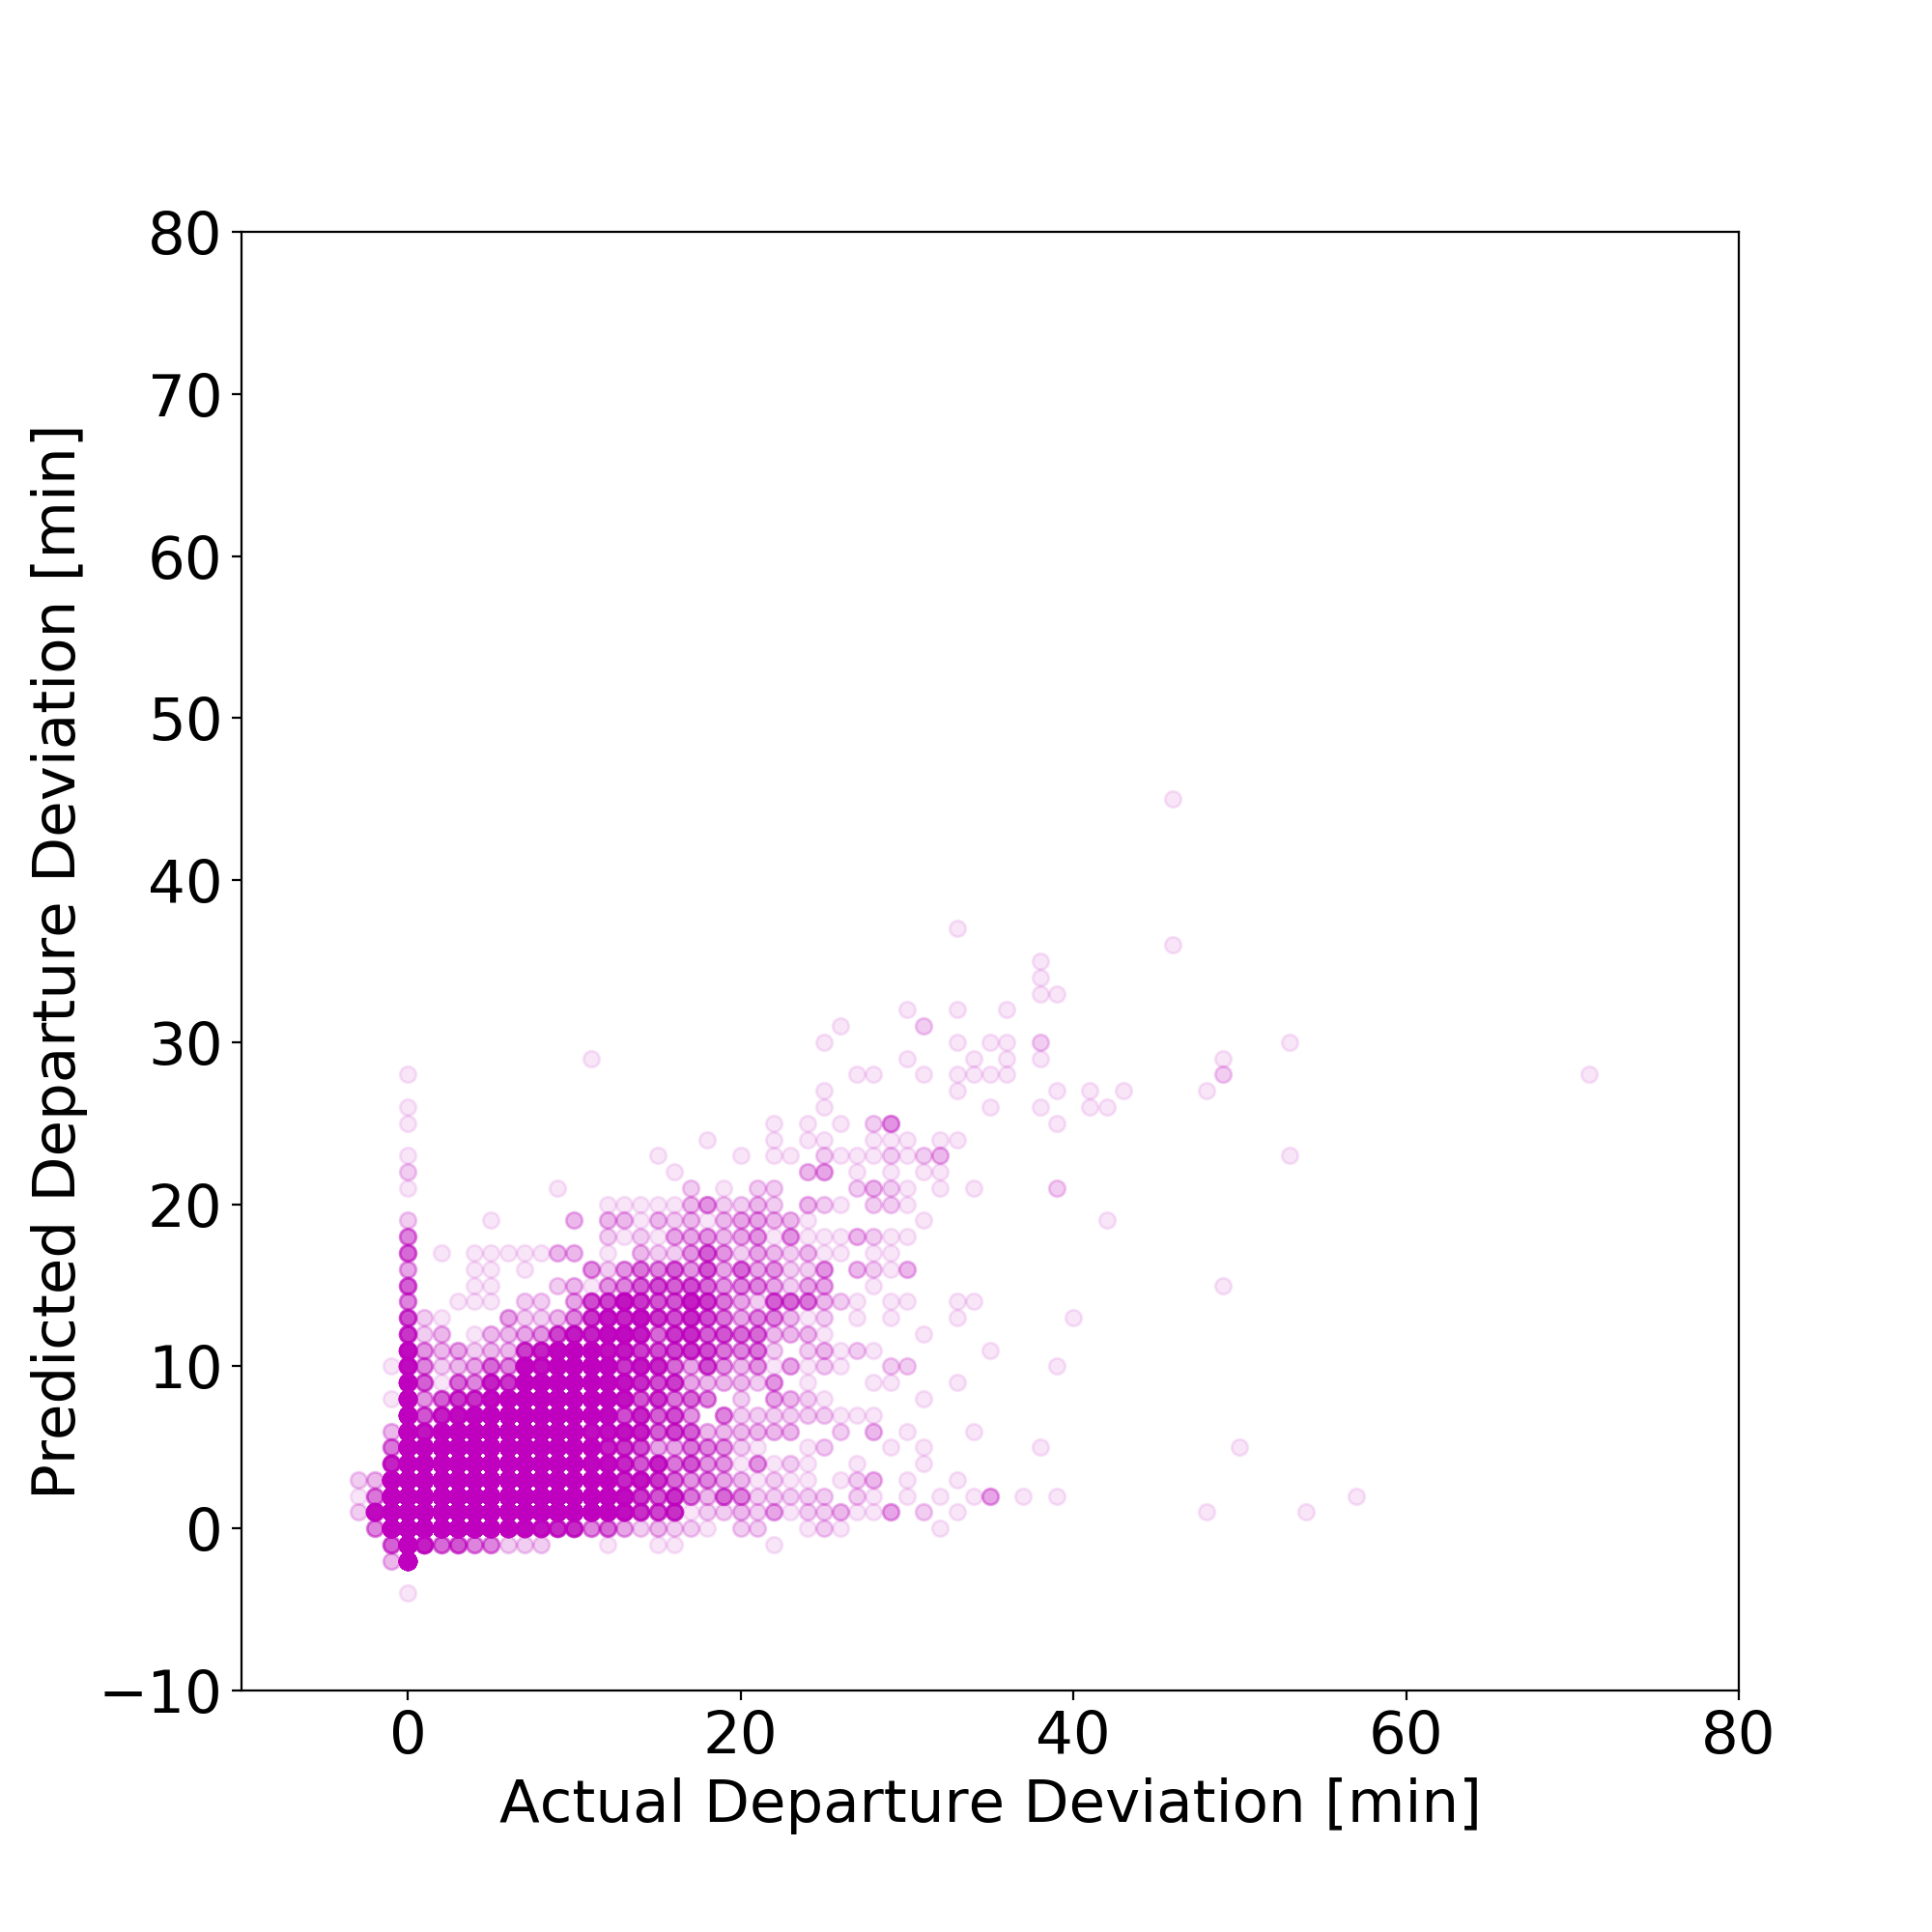
\includegraphics[width=0.5\textwidth]{Images/DNN_plot/5_step/5_step_depature_deviation.png}\label{fig:5_step_depature_deviation}}
\subfloat[\tiny{5-Step XGBoost Deviation from Departure}]{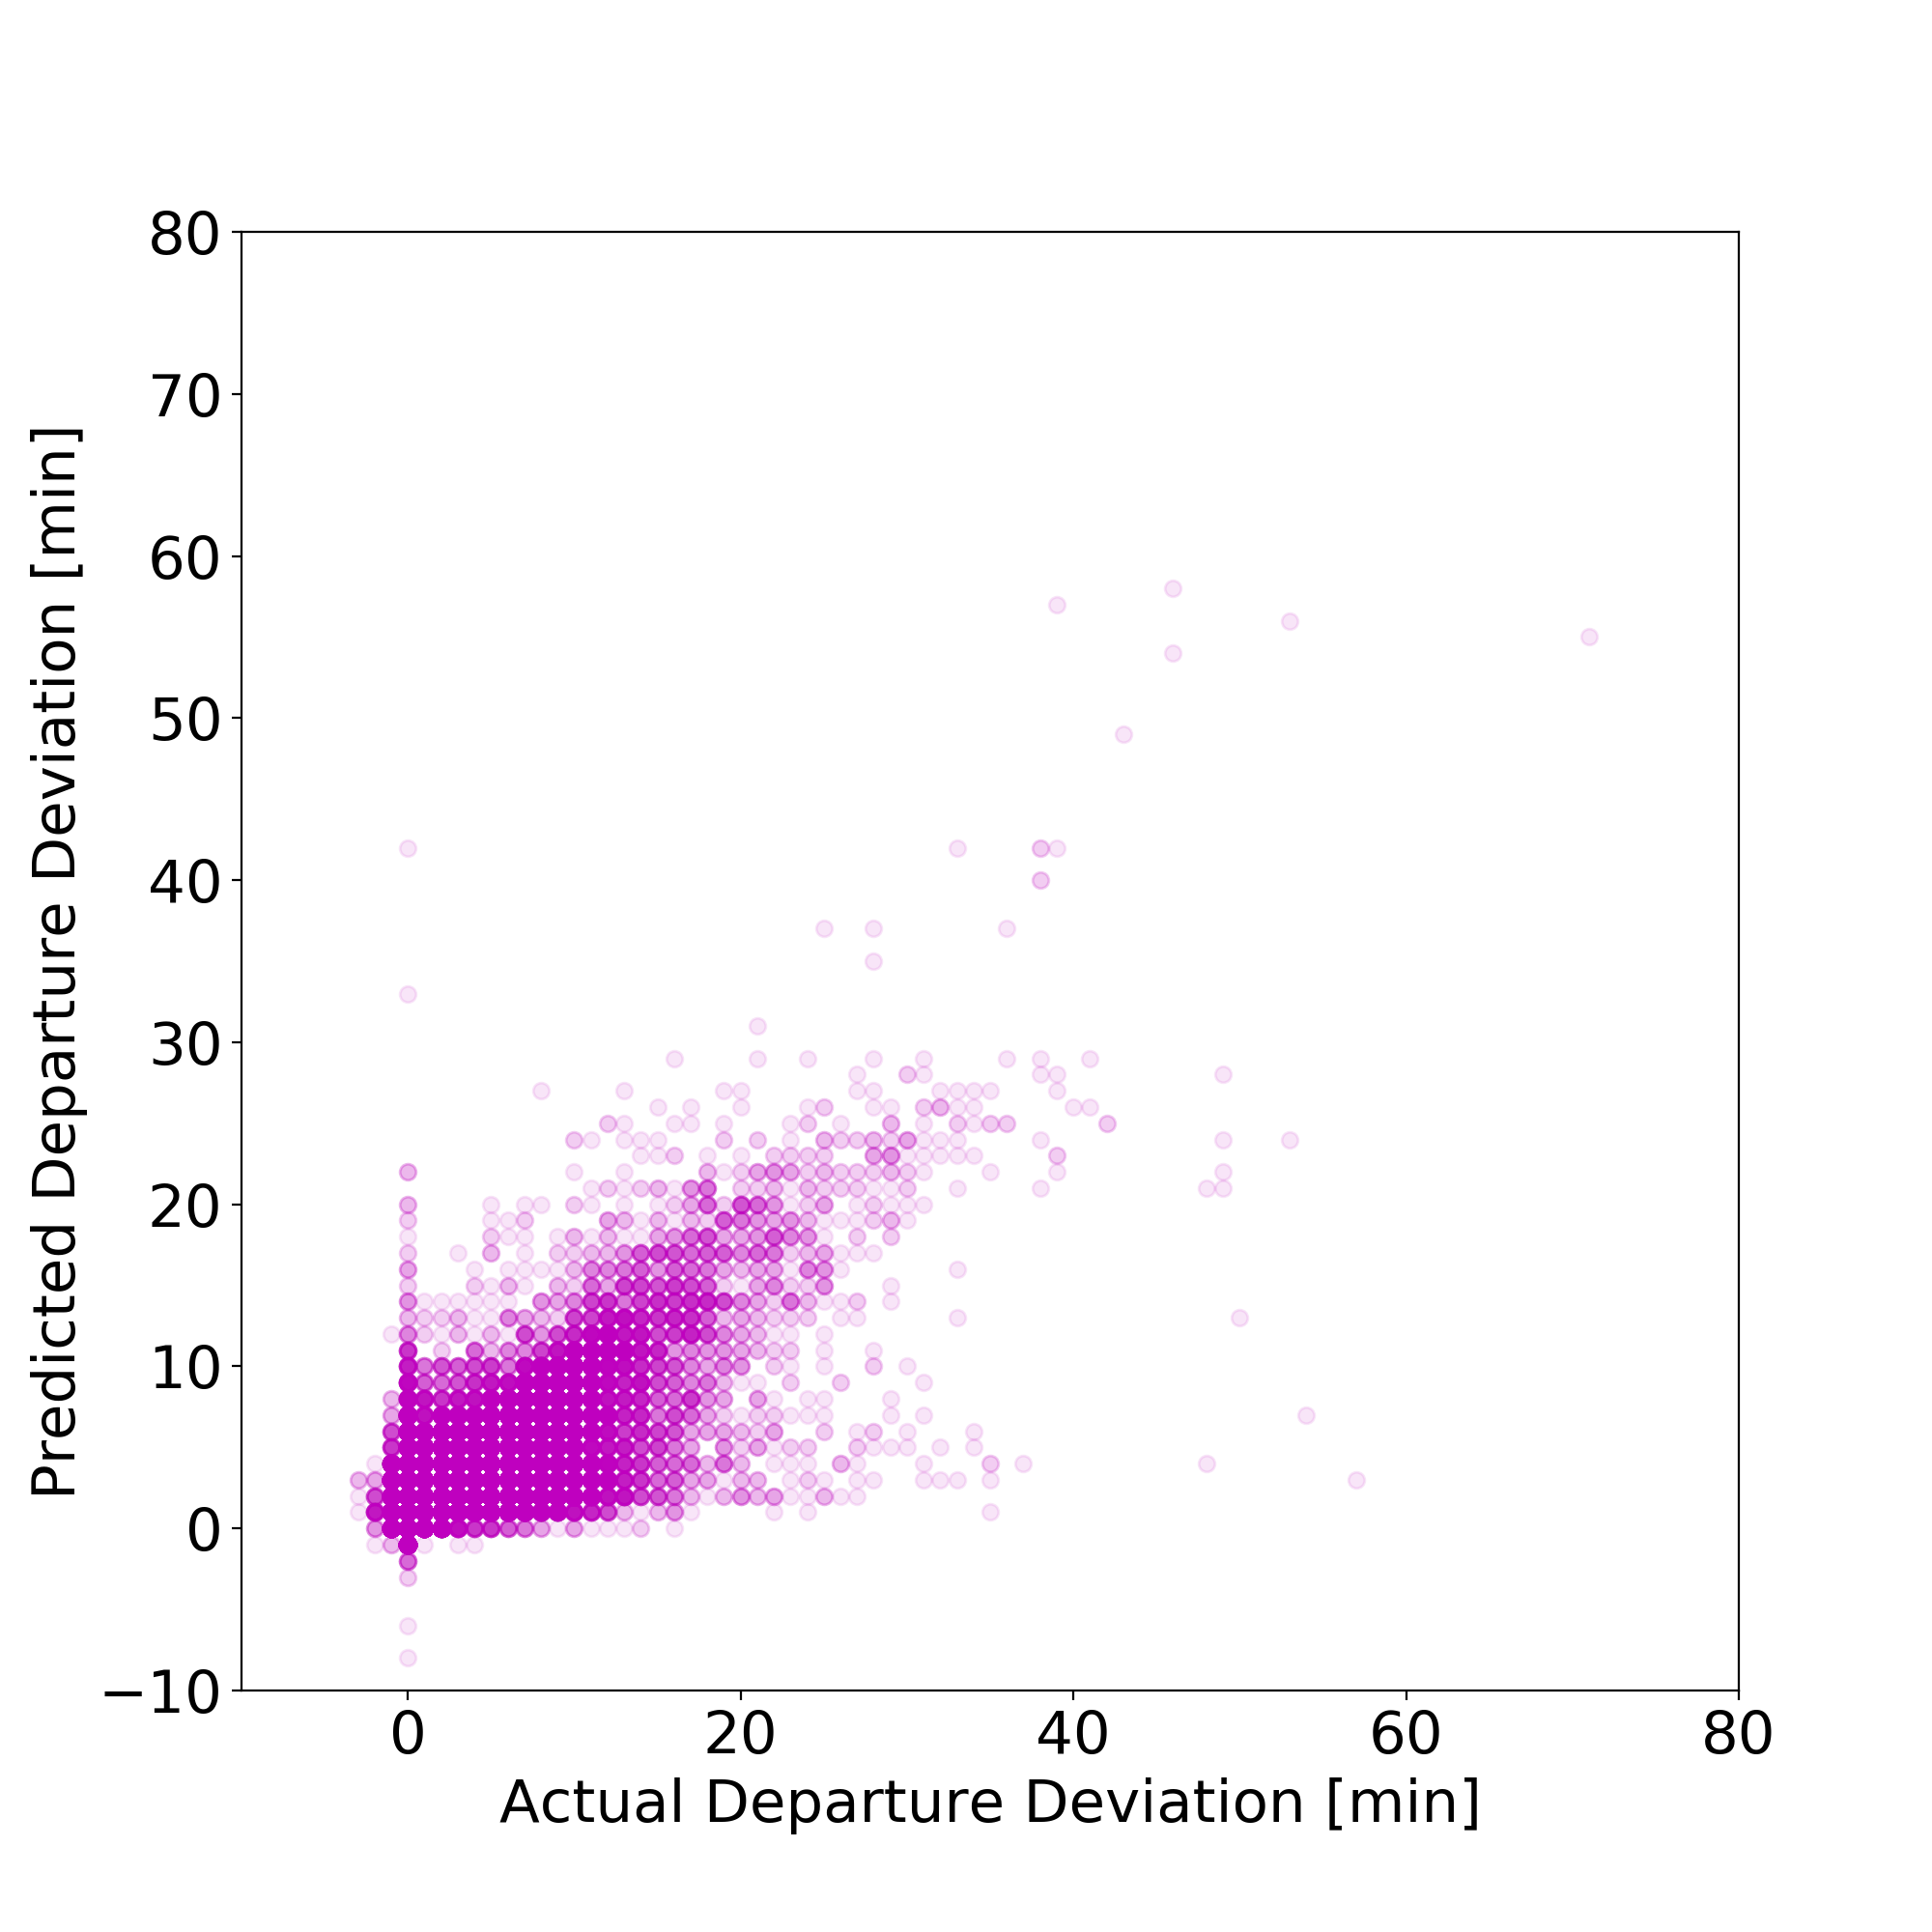
\includegraphics[width=0.5\textwidth]{Images/XGBoost_plot/5_step/5_step_depature_deviation.png}\label{fig:5_step_depature_deviation}}
\end{figure}
\begin{figure}[H]
\centering
\subfloat[\tiny{5-Step DNN Travel Time}]{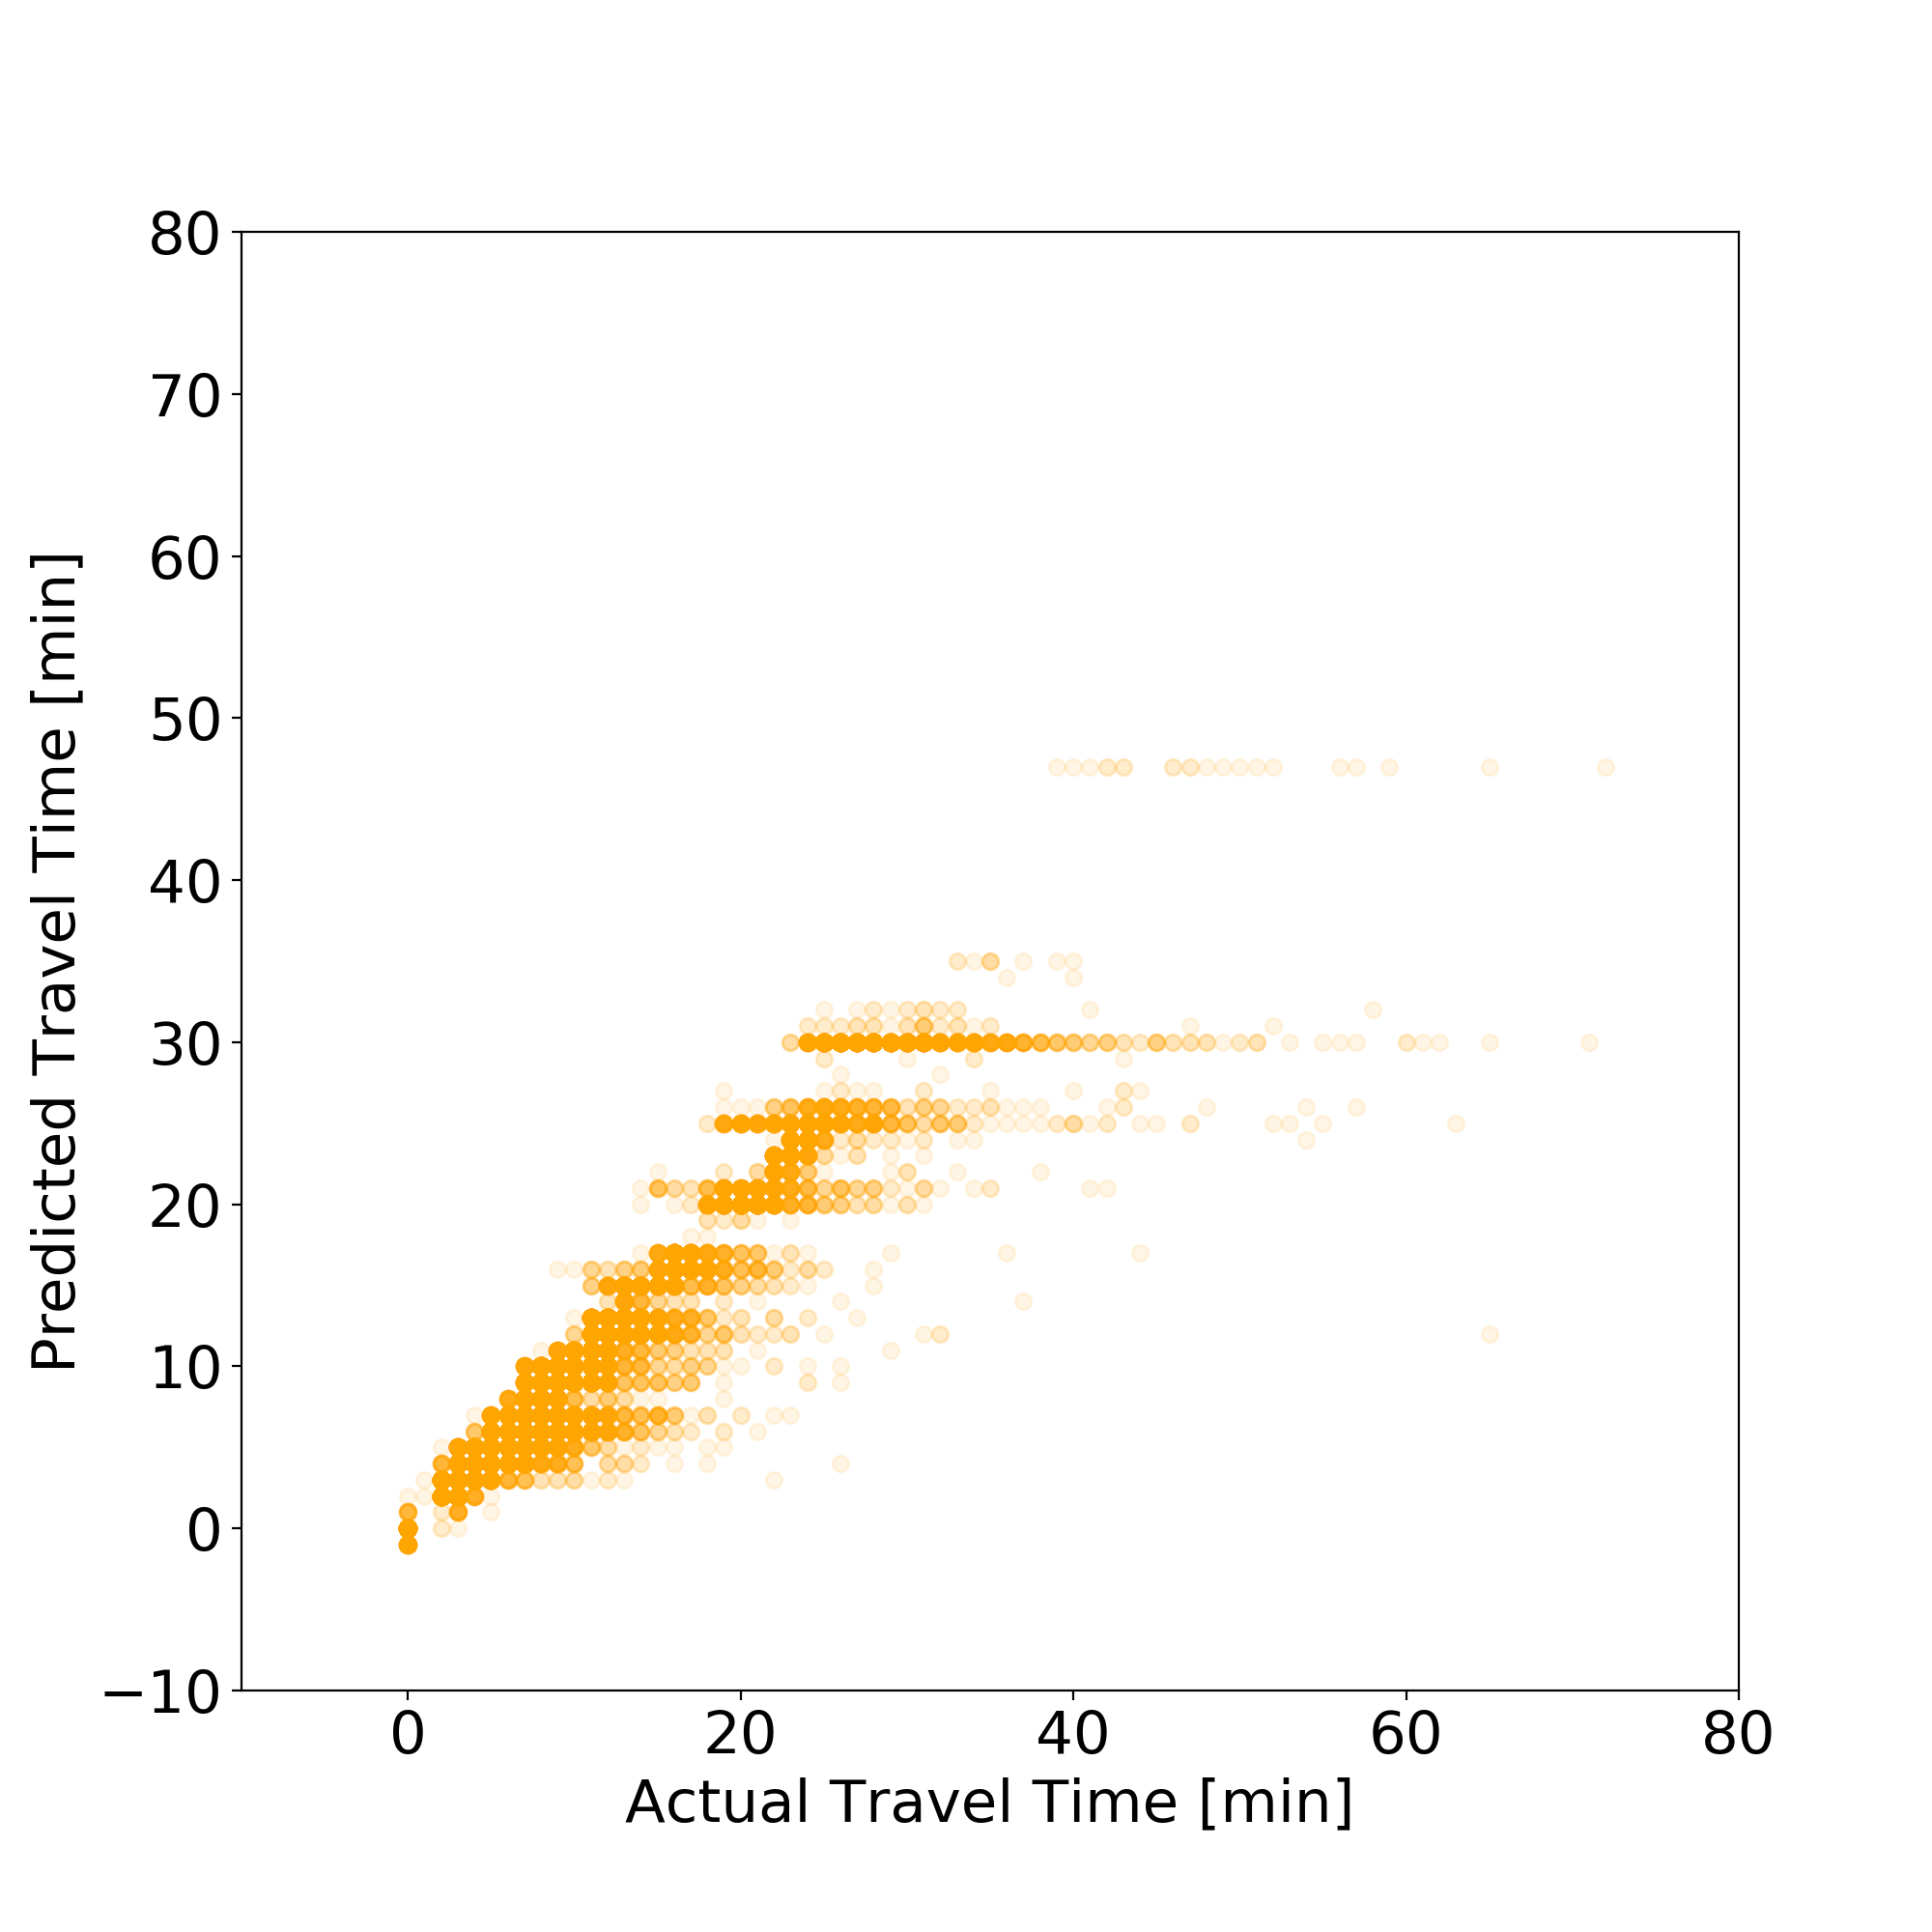
\includegraphics[width=0.5\textwidth]{Images/DNN_plot/5_step/5_step_travel_time.png}\label{fig:5_step_travel_time}}
\subfloat[\tiny{5-Step XGBoost Travel Time}]{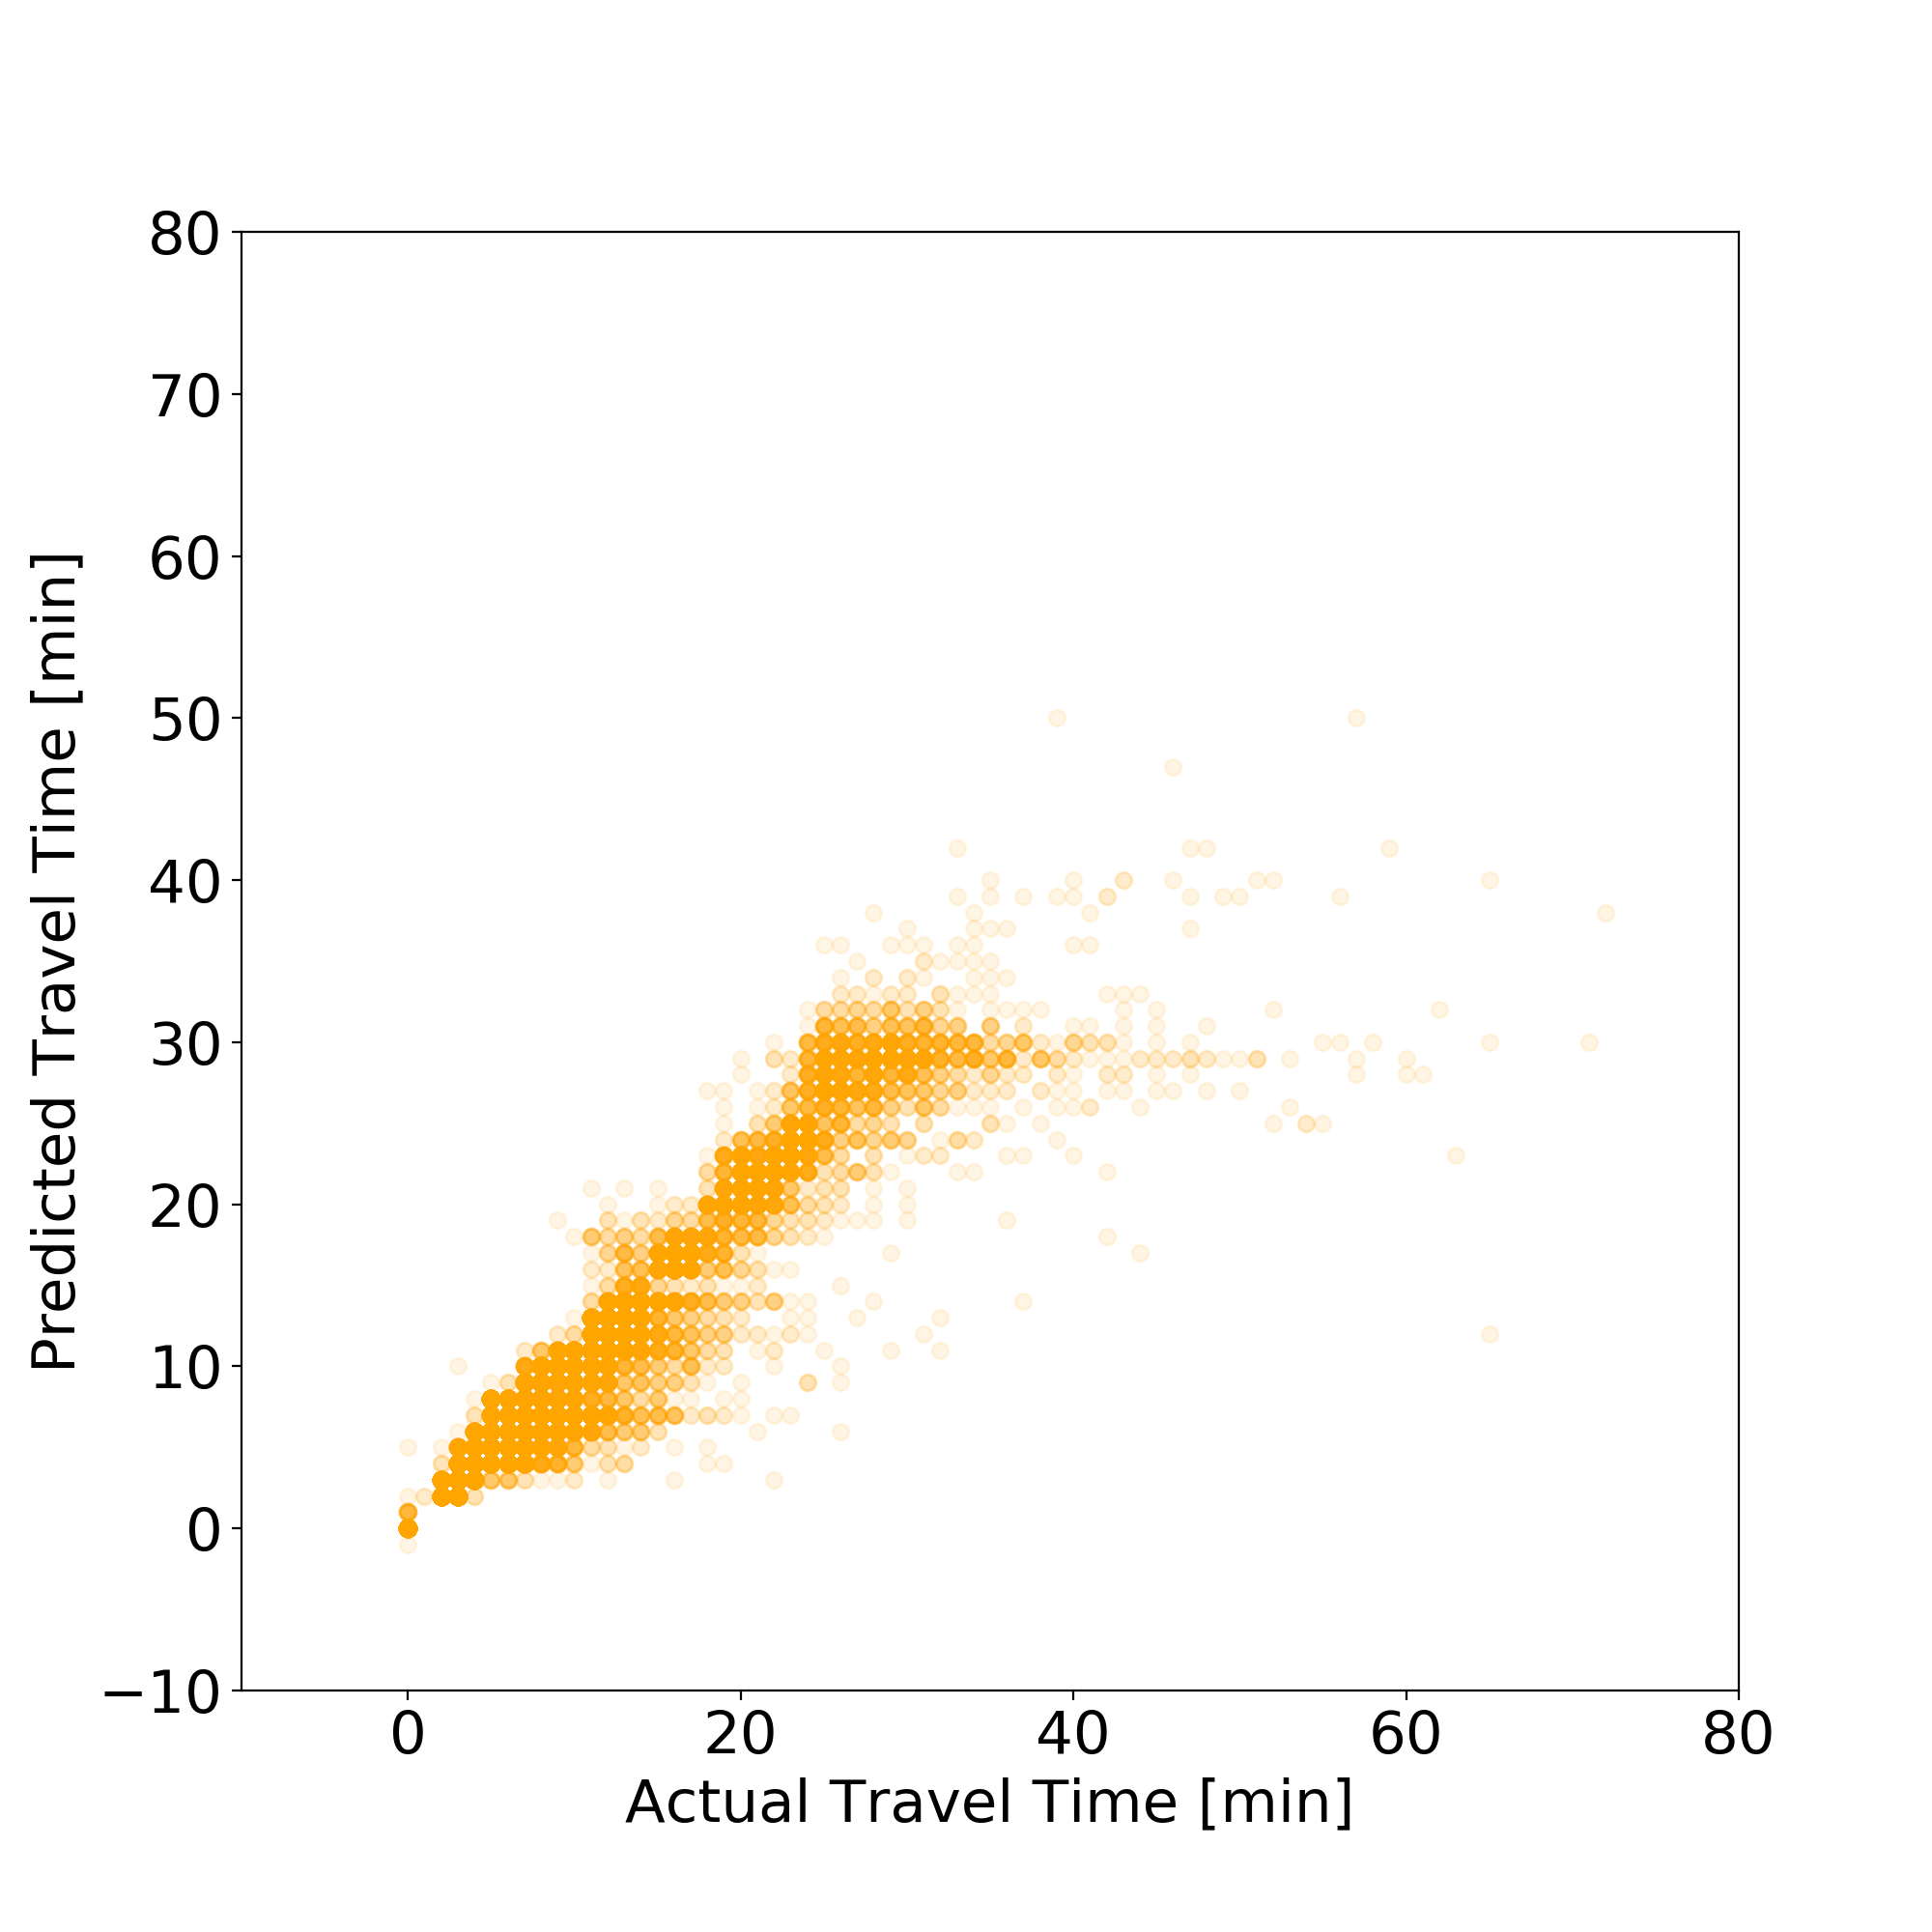
\includegraphics[width=0.5\textwidth]{Images/XGBoost_plot/5_step/5_step_travel_time.png}\label{fig:5_step_travel_time}}
\end{figure}
\begin{figure}[H]
\centering
\subfloat[\tiny{5-Step DNN Dwell Time}]{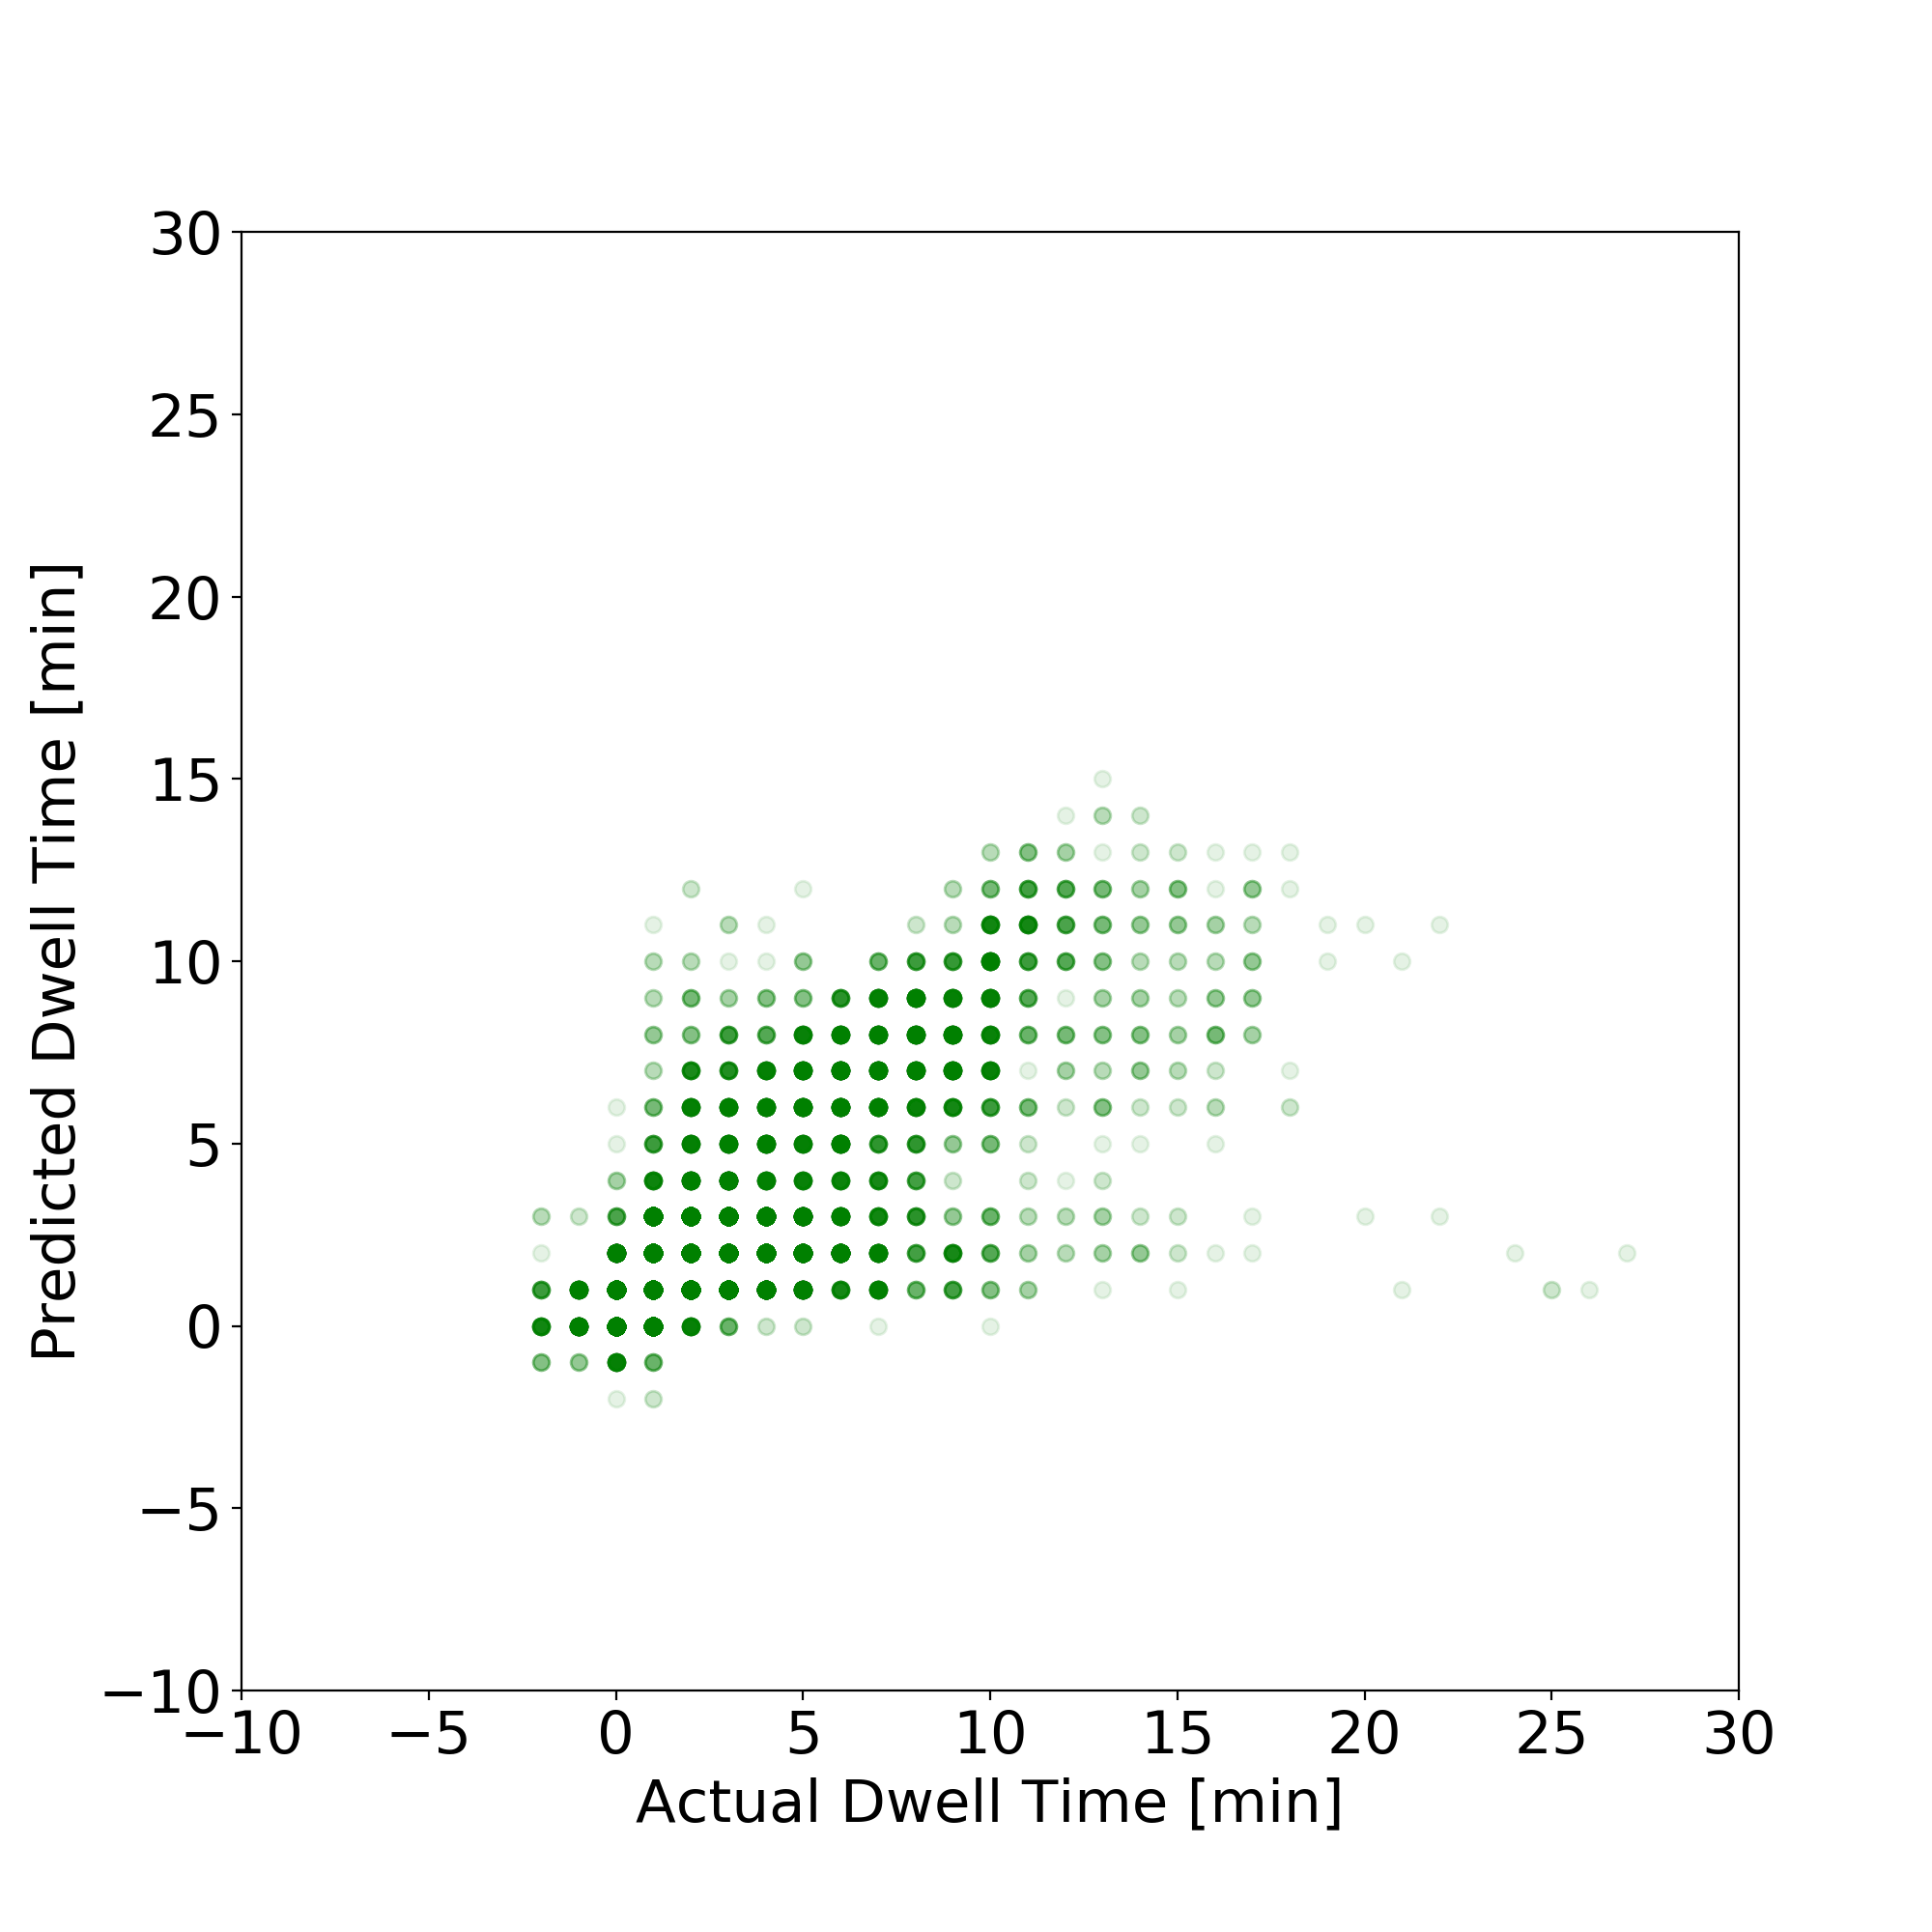
\includegraphics[width=0.5\textwidth]{Images/DNN_plot/5_step/5_step_dwell_time.png}\label{fig:5_step_dwell_time}}
\subfloat[\tiny{5-Step XGBoost Dwell Time}]{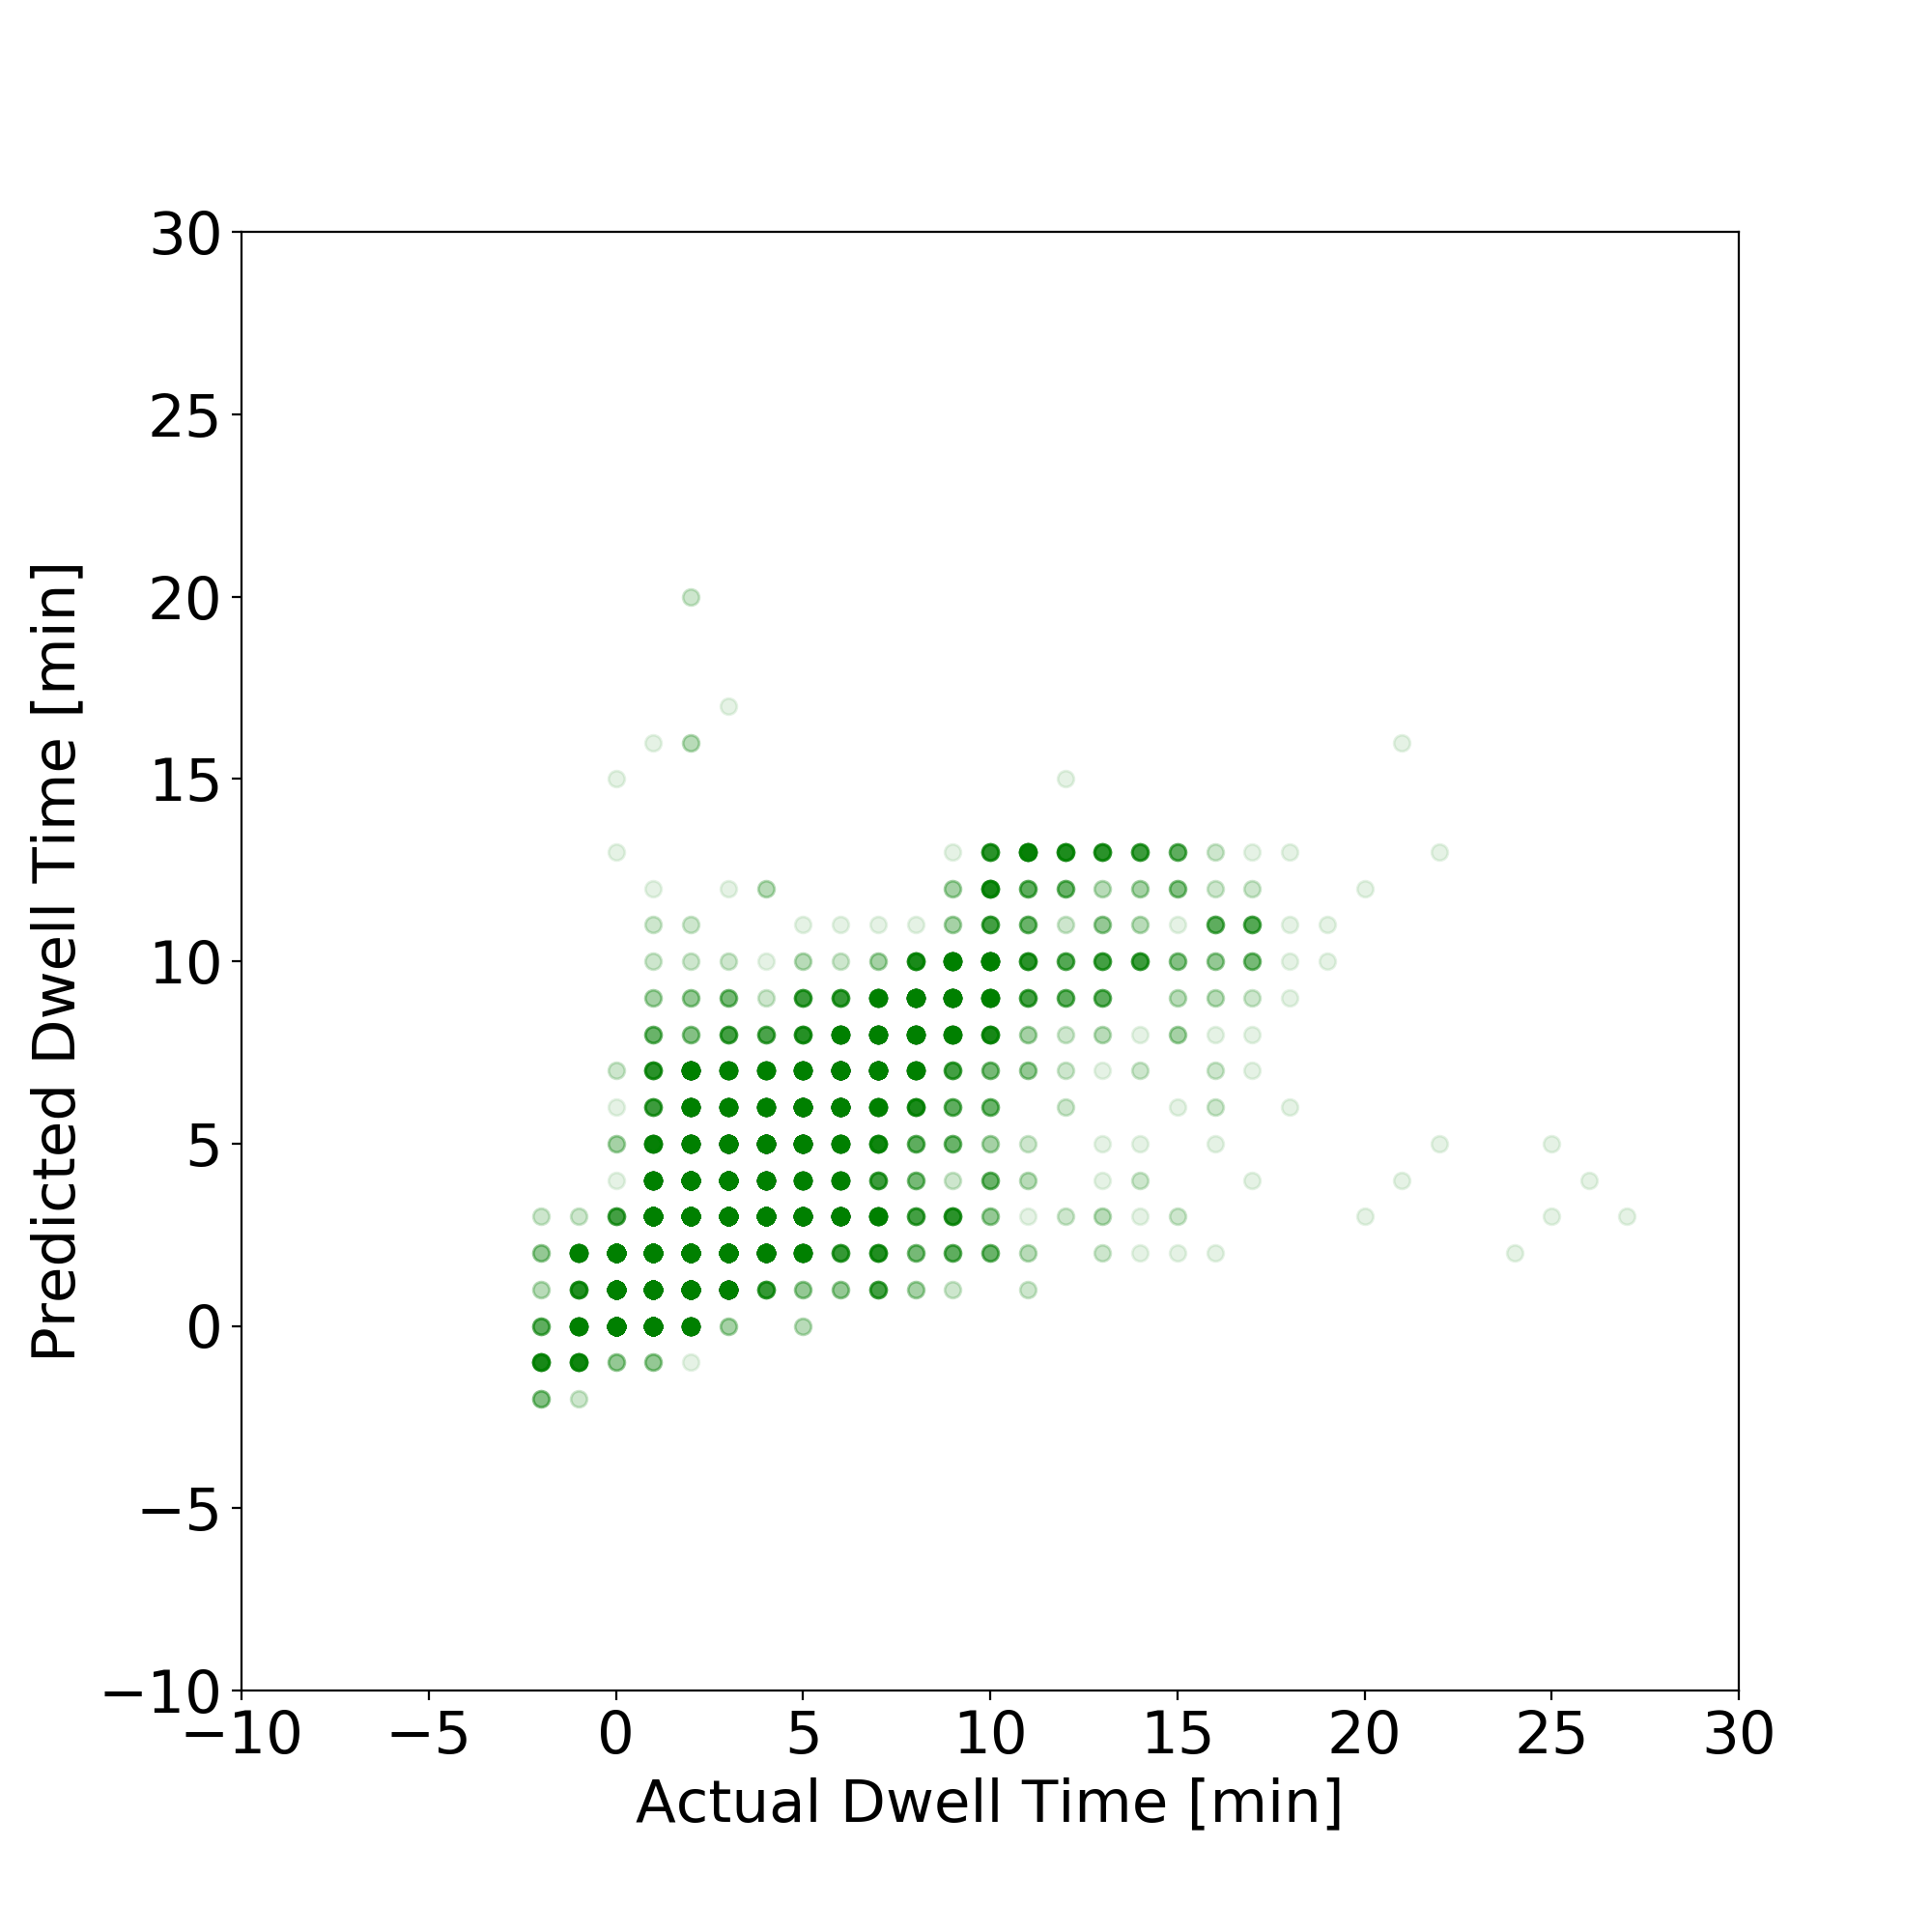
\includegraphics[width=0.5\textwidth]{Images/XGBoost_plot/5_step/5_step_dwell_time.png}\label{fig:5_step_dwell_time}}
\end{figure}

\begin{figure}[H]
\centering
\subfloat[\tiny{6-Step DNN Deviation from Arrival}]{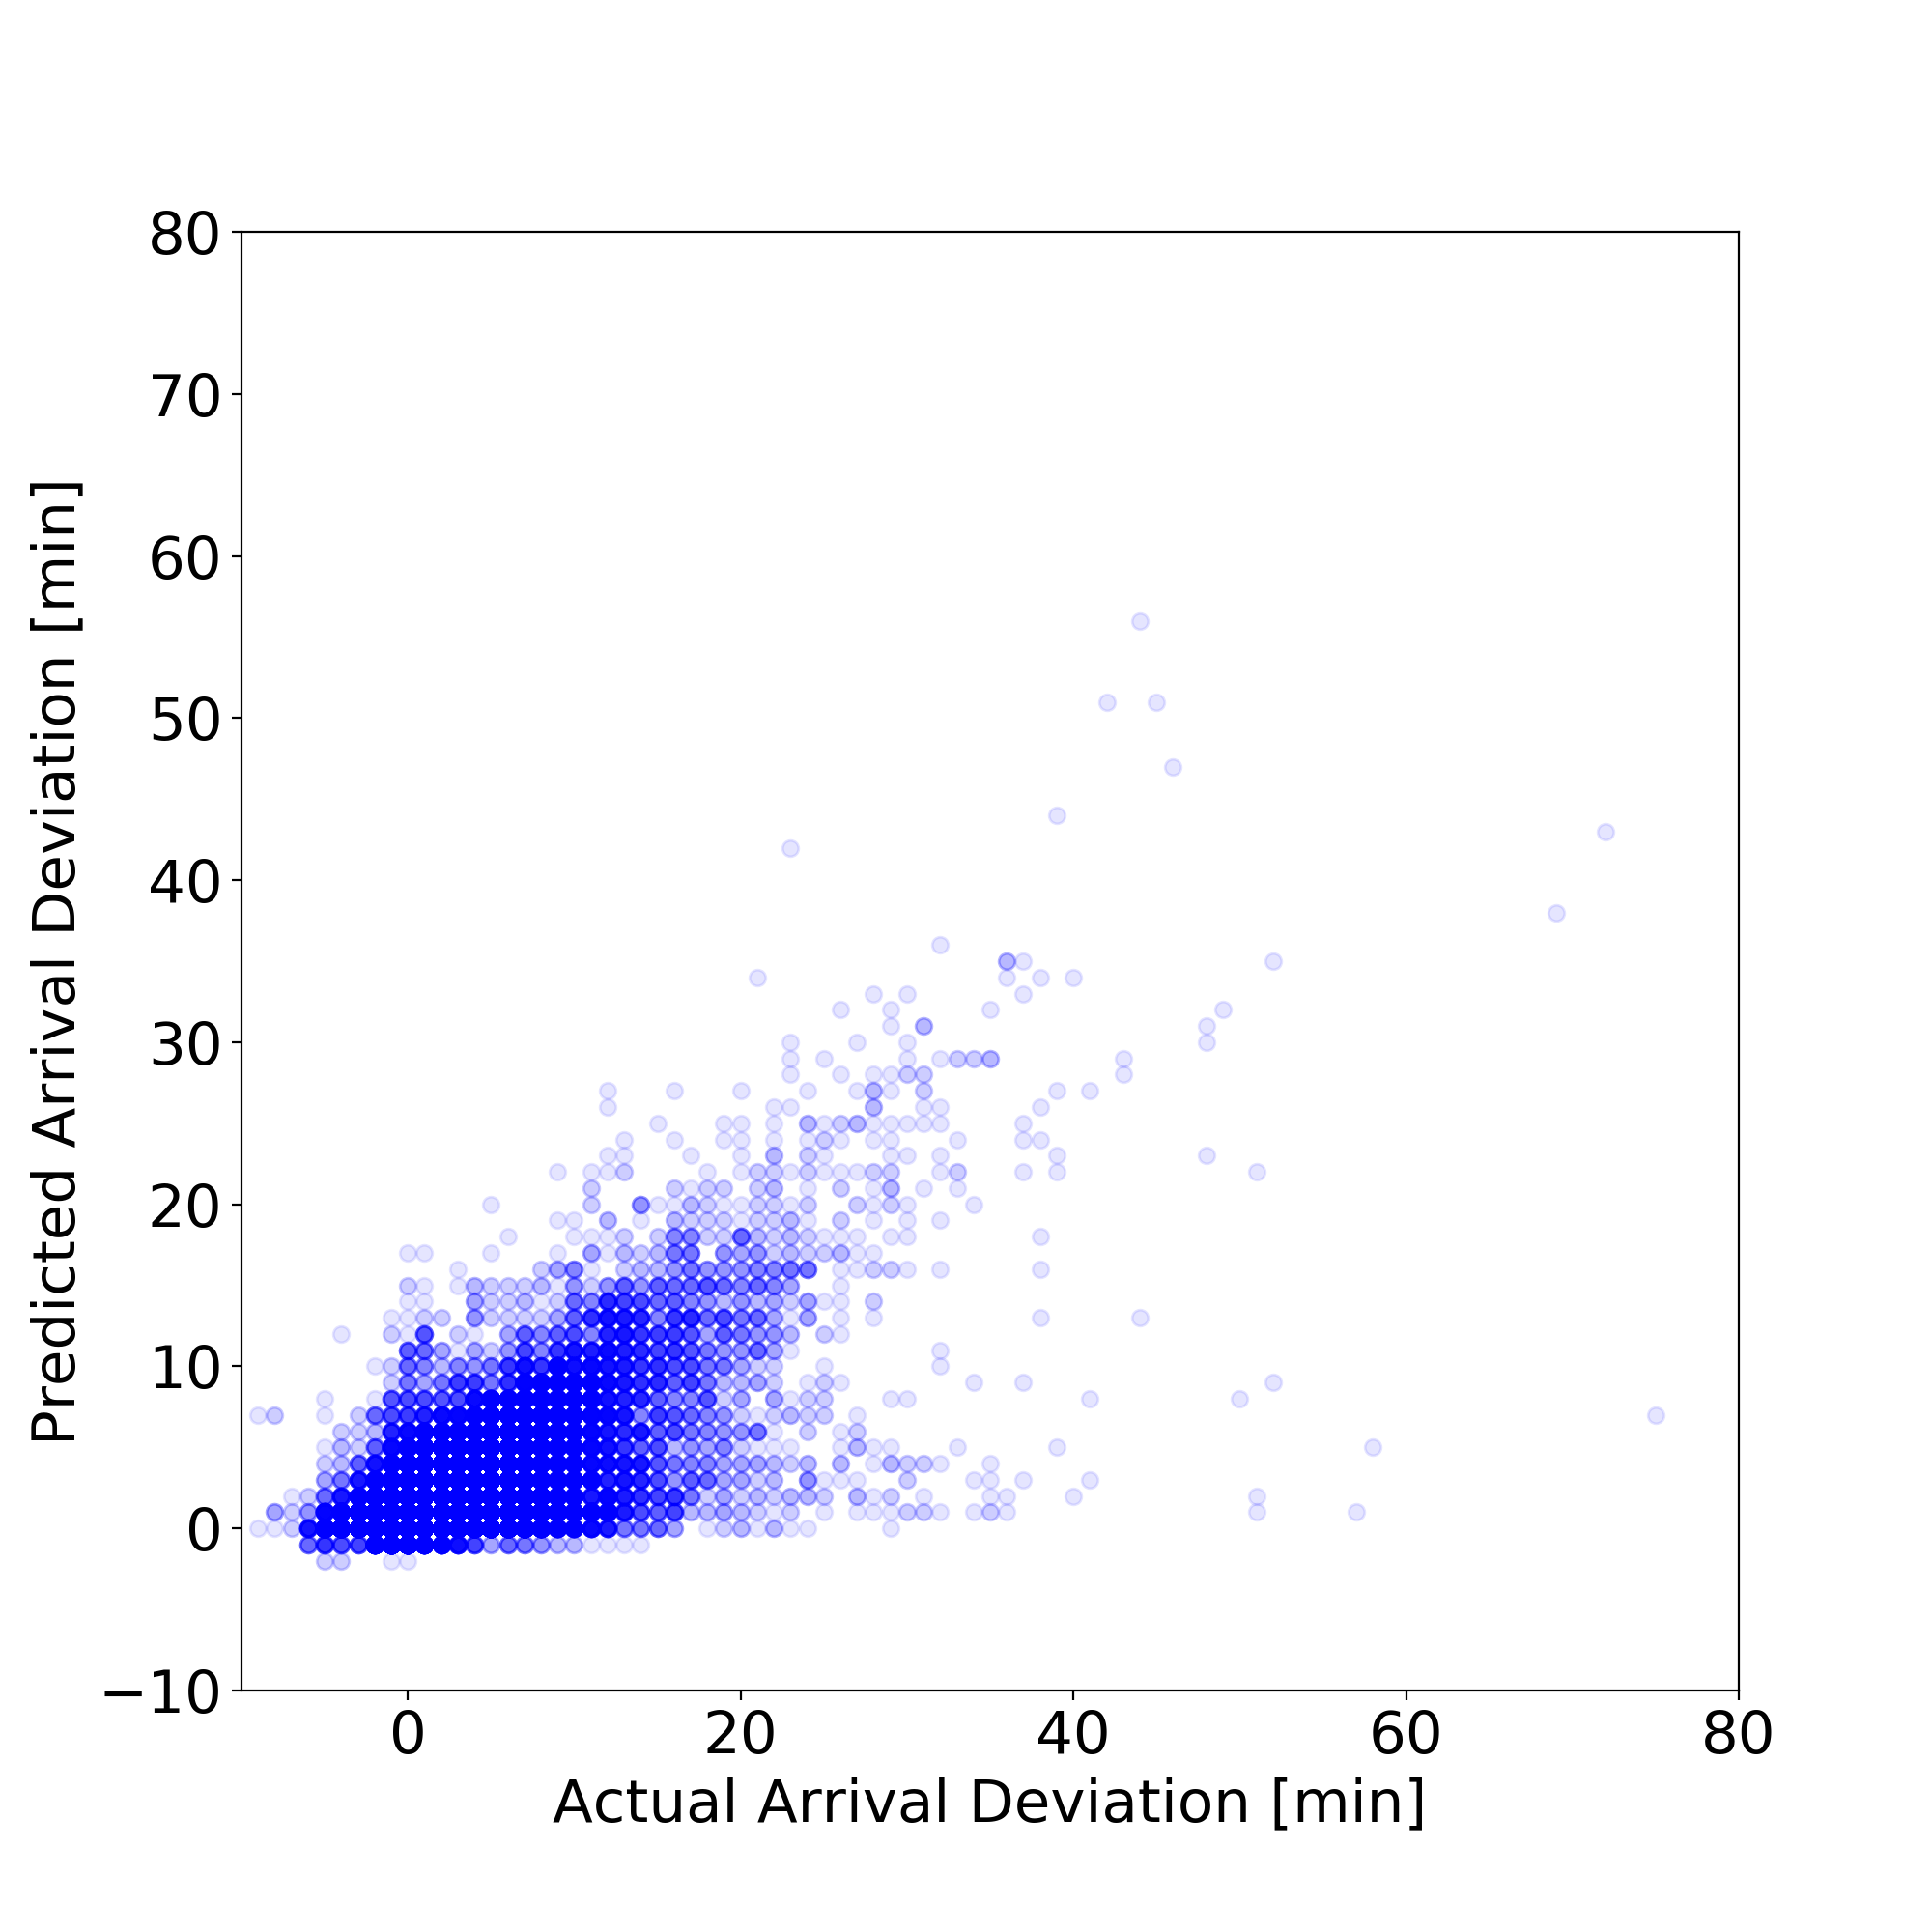
\includegraphics[width=0.5\textwidth]{Images/DNN_plot/6_step/6_step_arrival_deviation.png}\label{fig:6_step_arrival_deviation}}
\subfloat[\tiny{6-Step XGBoost Deviation from Arrival}]{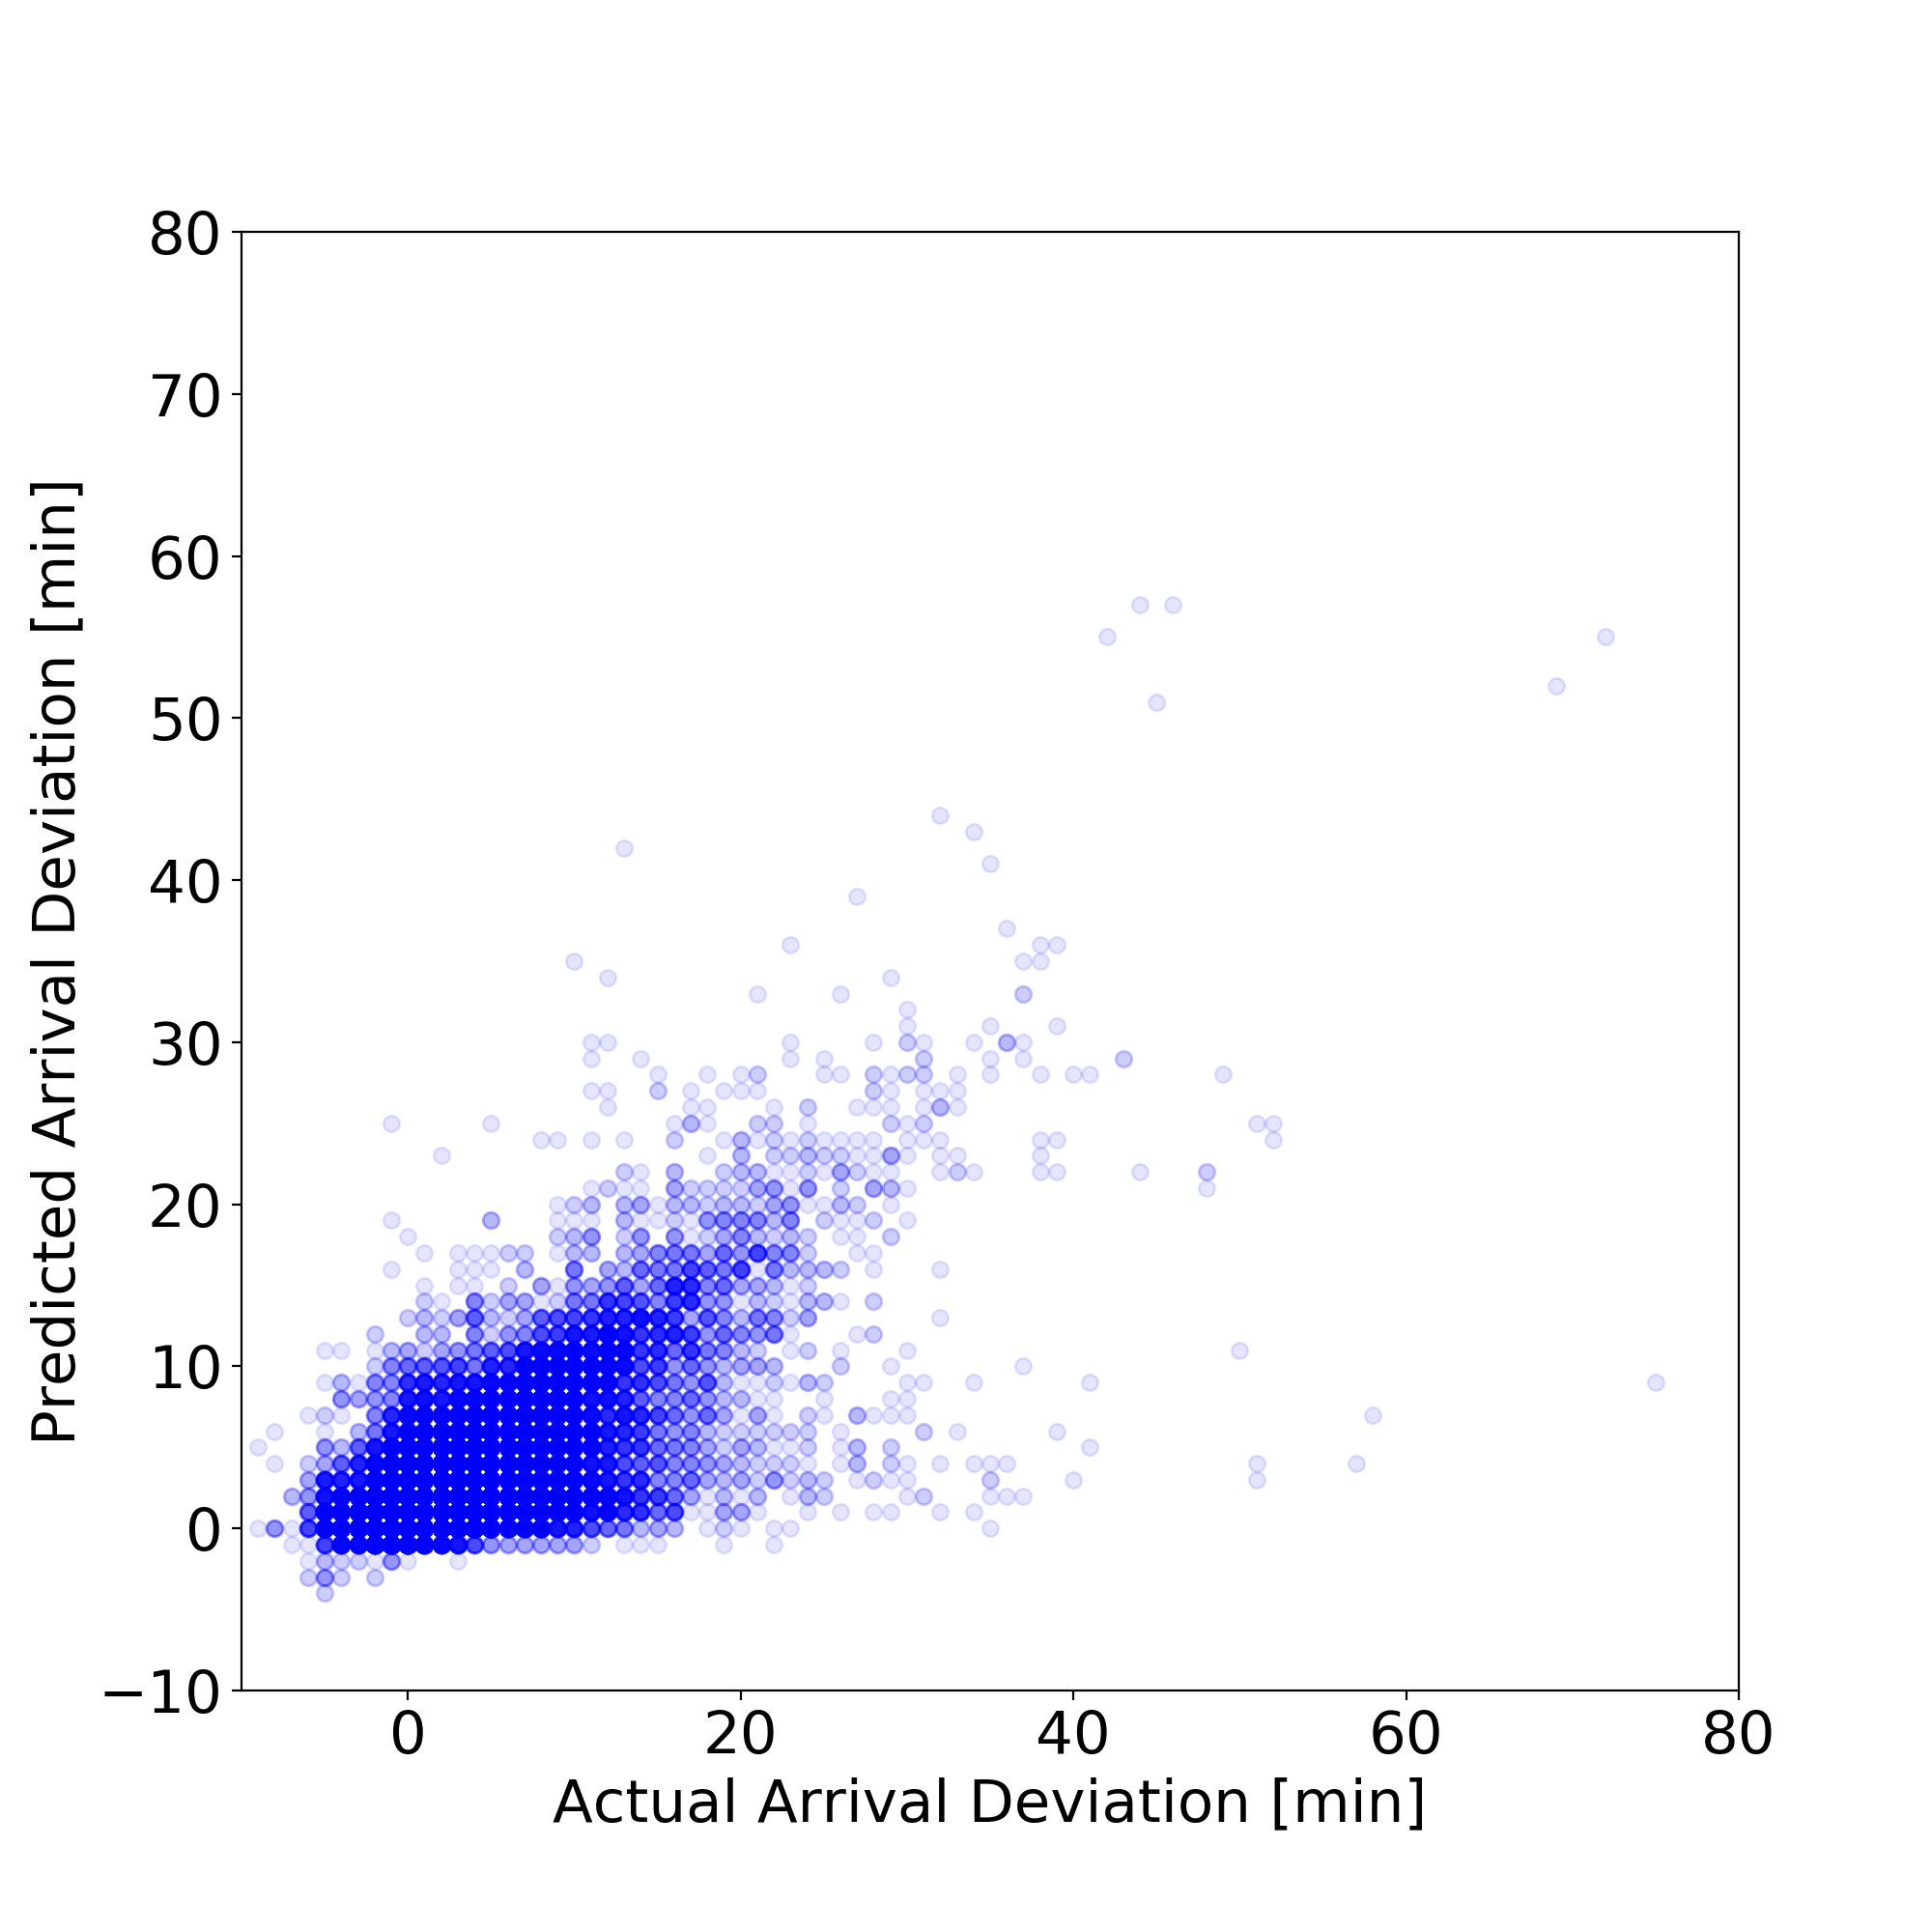
\includegraphics[width=0.5\textwidth]{Images/XGBoost_plot/6_step/6_step_arrival_deviation.png}\label{fig:6_step_arrival_deviation}}
\end{figure}
\begin{figure}[H]
\centering
\subfloat[\tiny{6-Step DNN Deviation from Departure}]{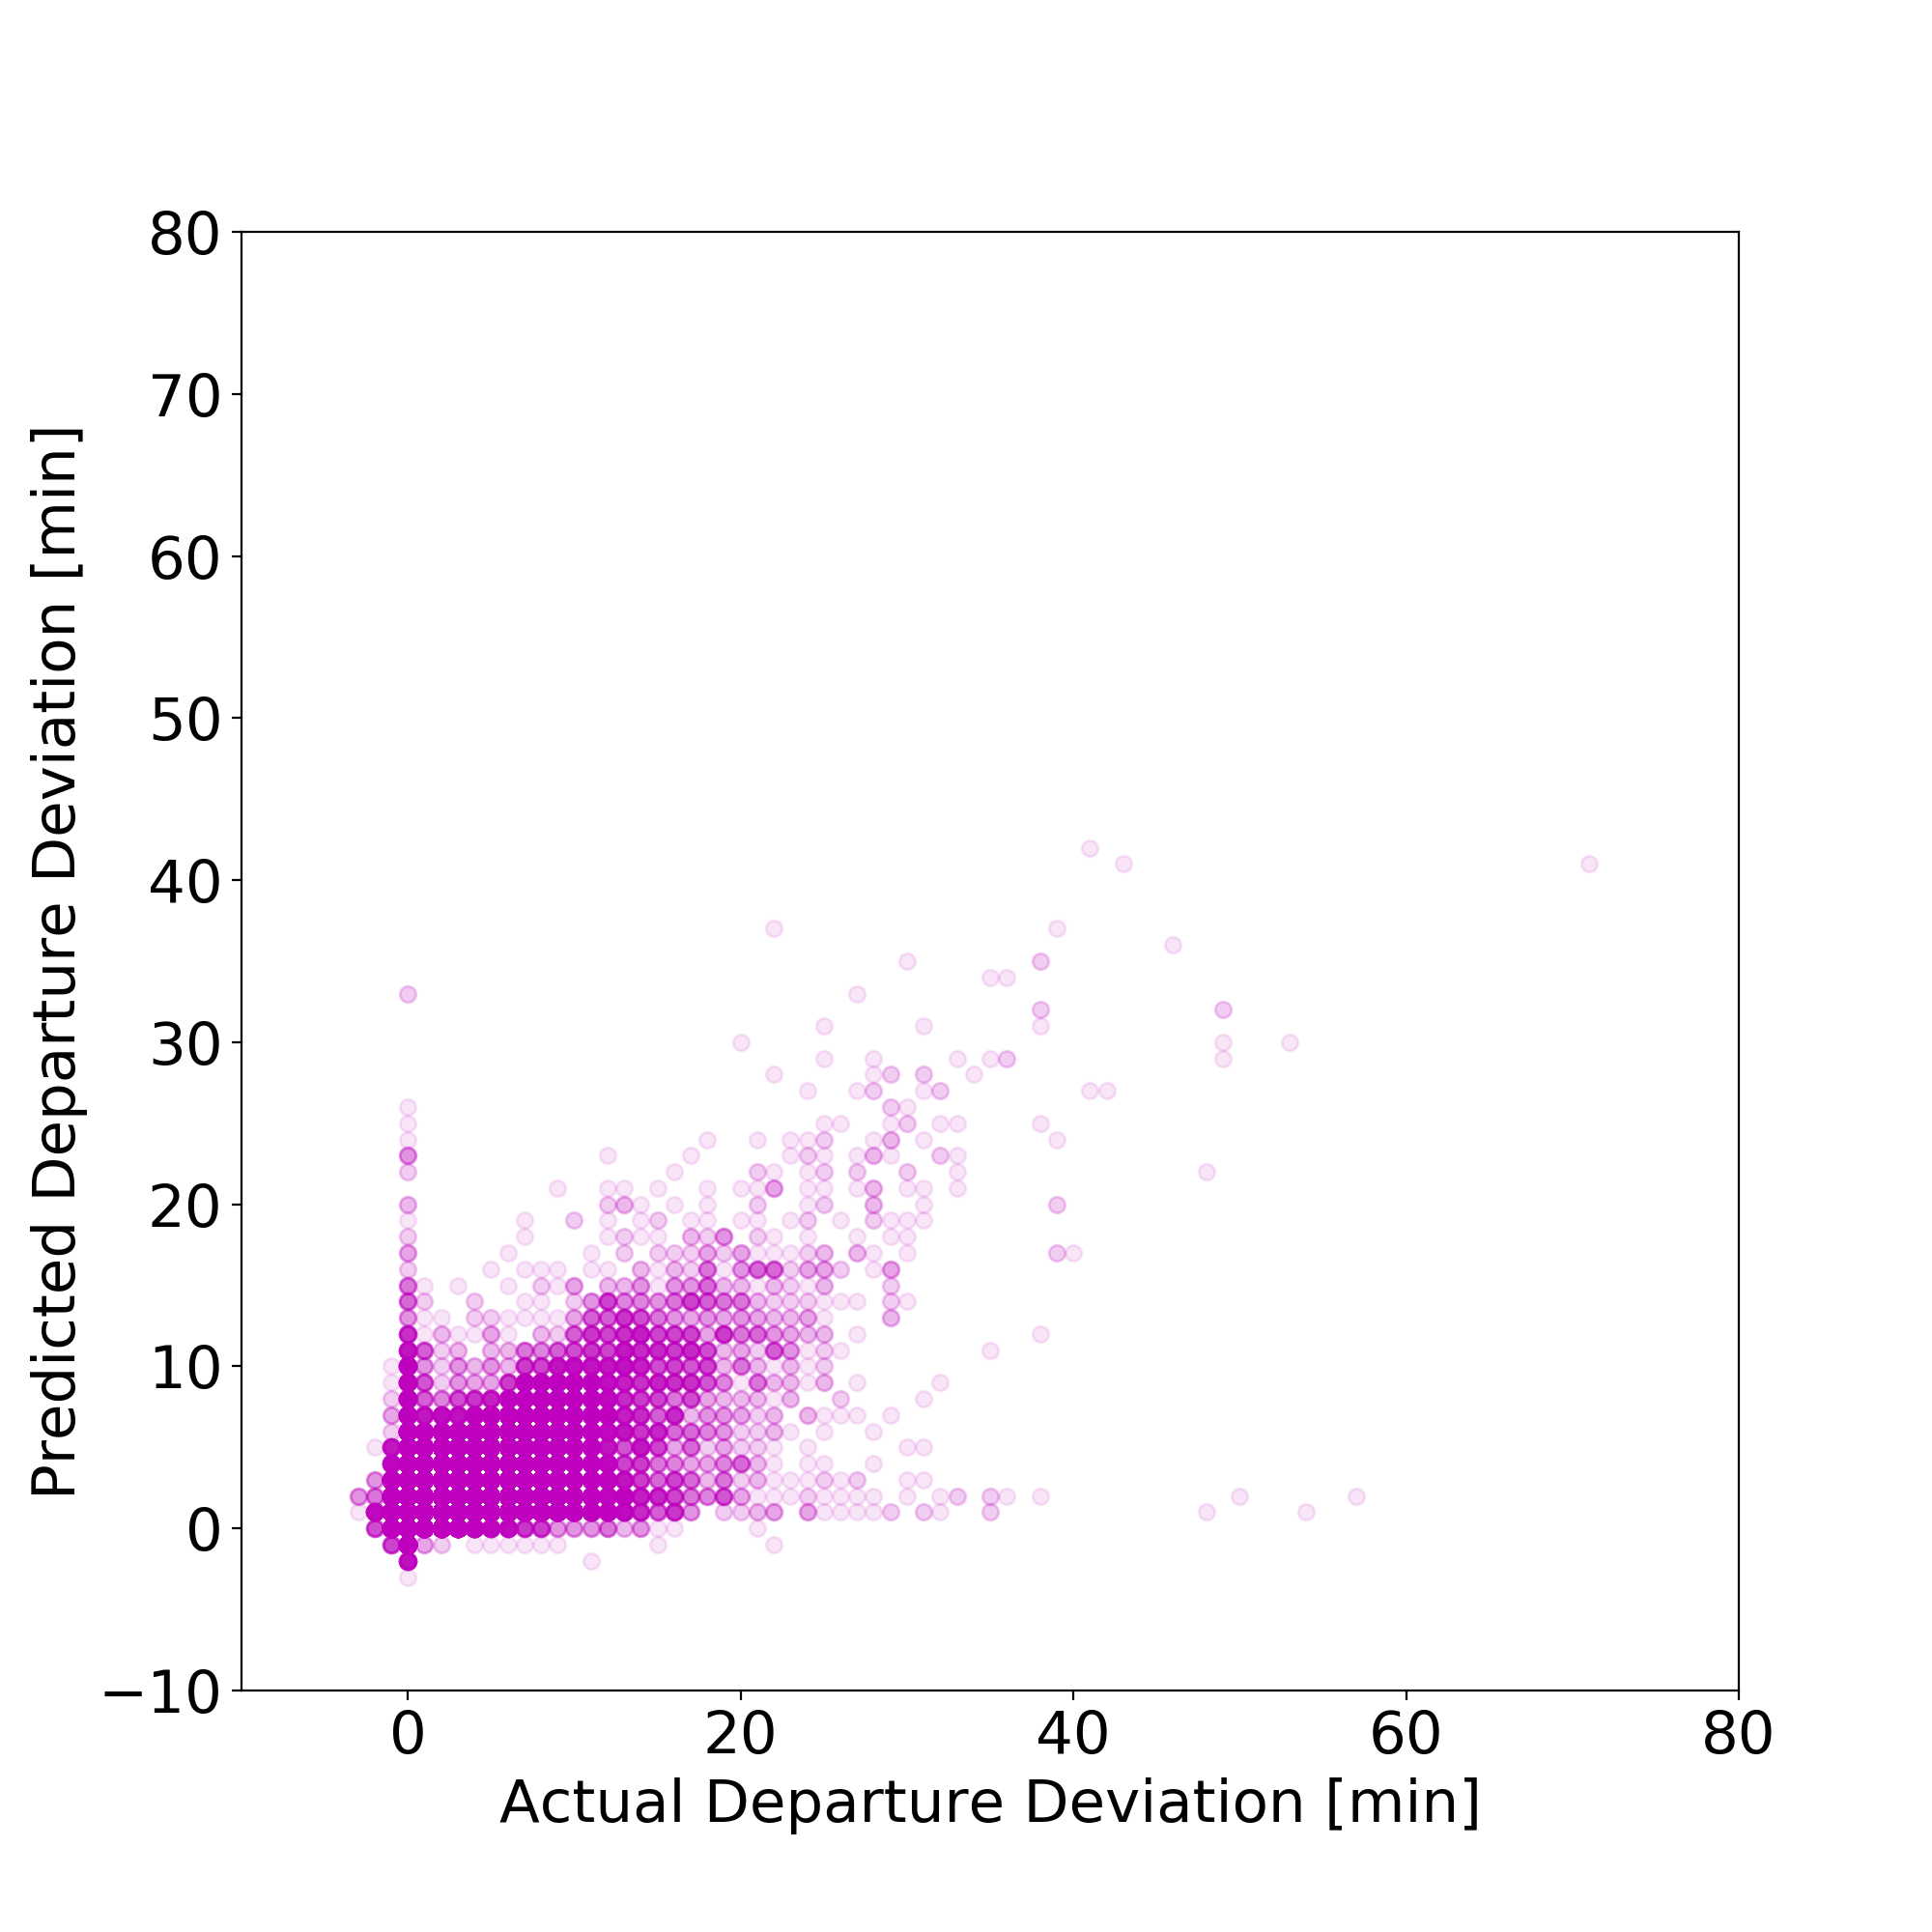
\includegraphics[width=0.5\textwidth]{Images/DNN_plot/6_step/6_step_depature_deviation.png}\label{fig:6_step_depature_deviation}}
\subfloat[\tiny{6-Step XGBoost Deviation from Departure}]{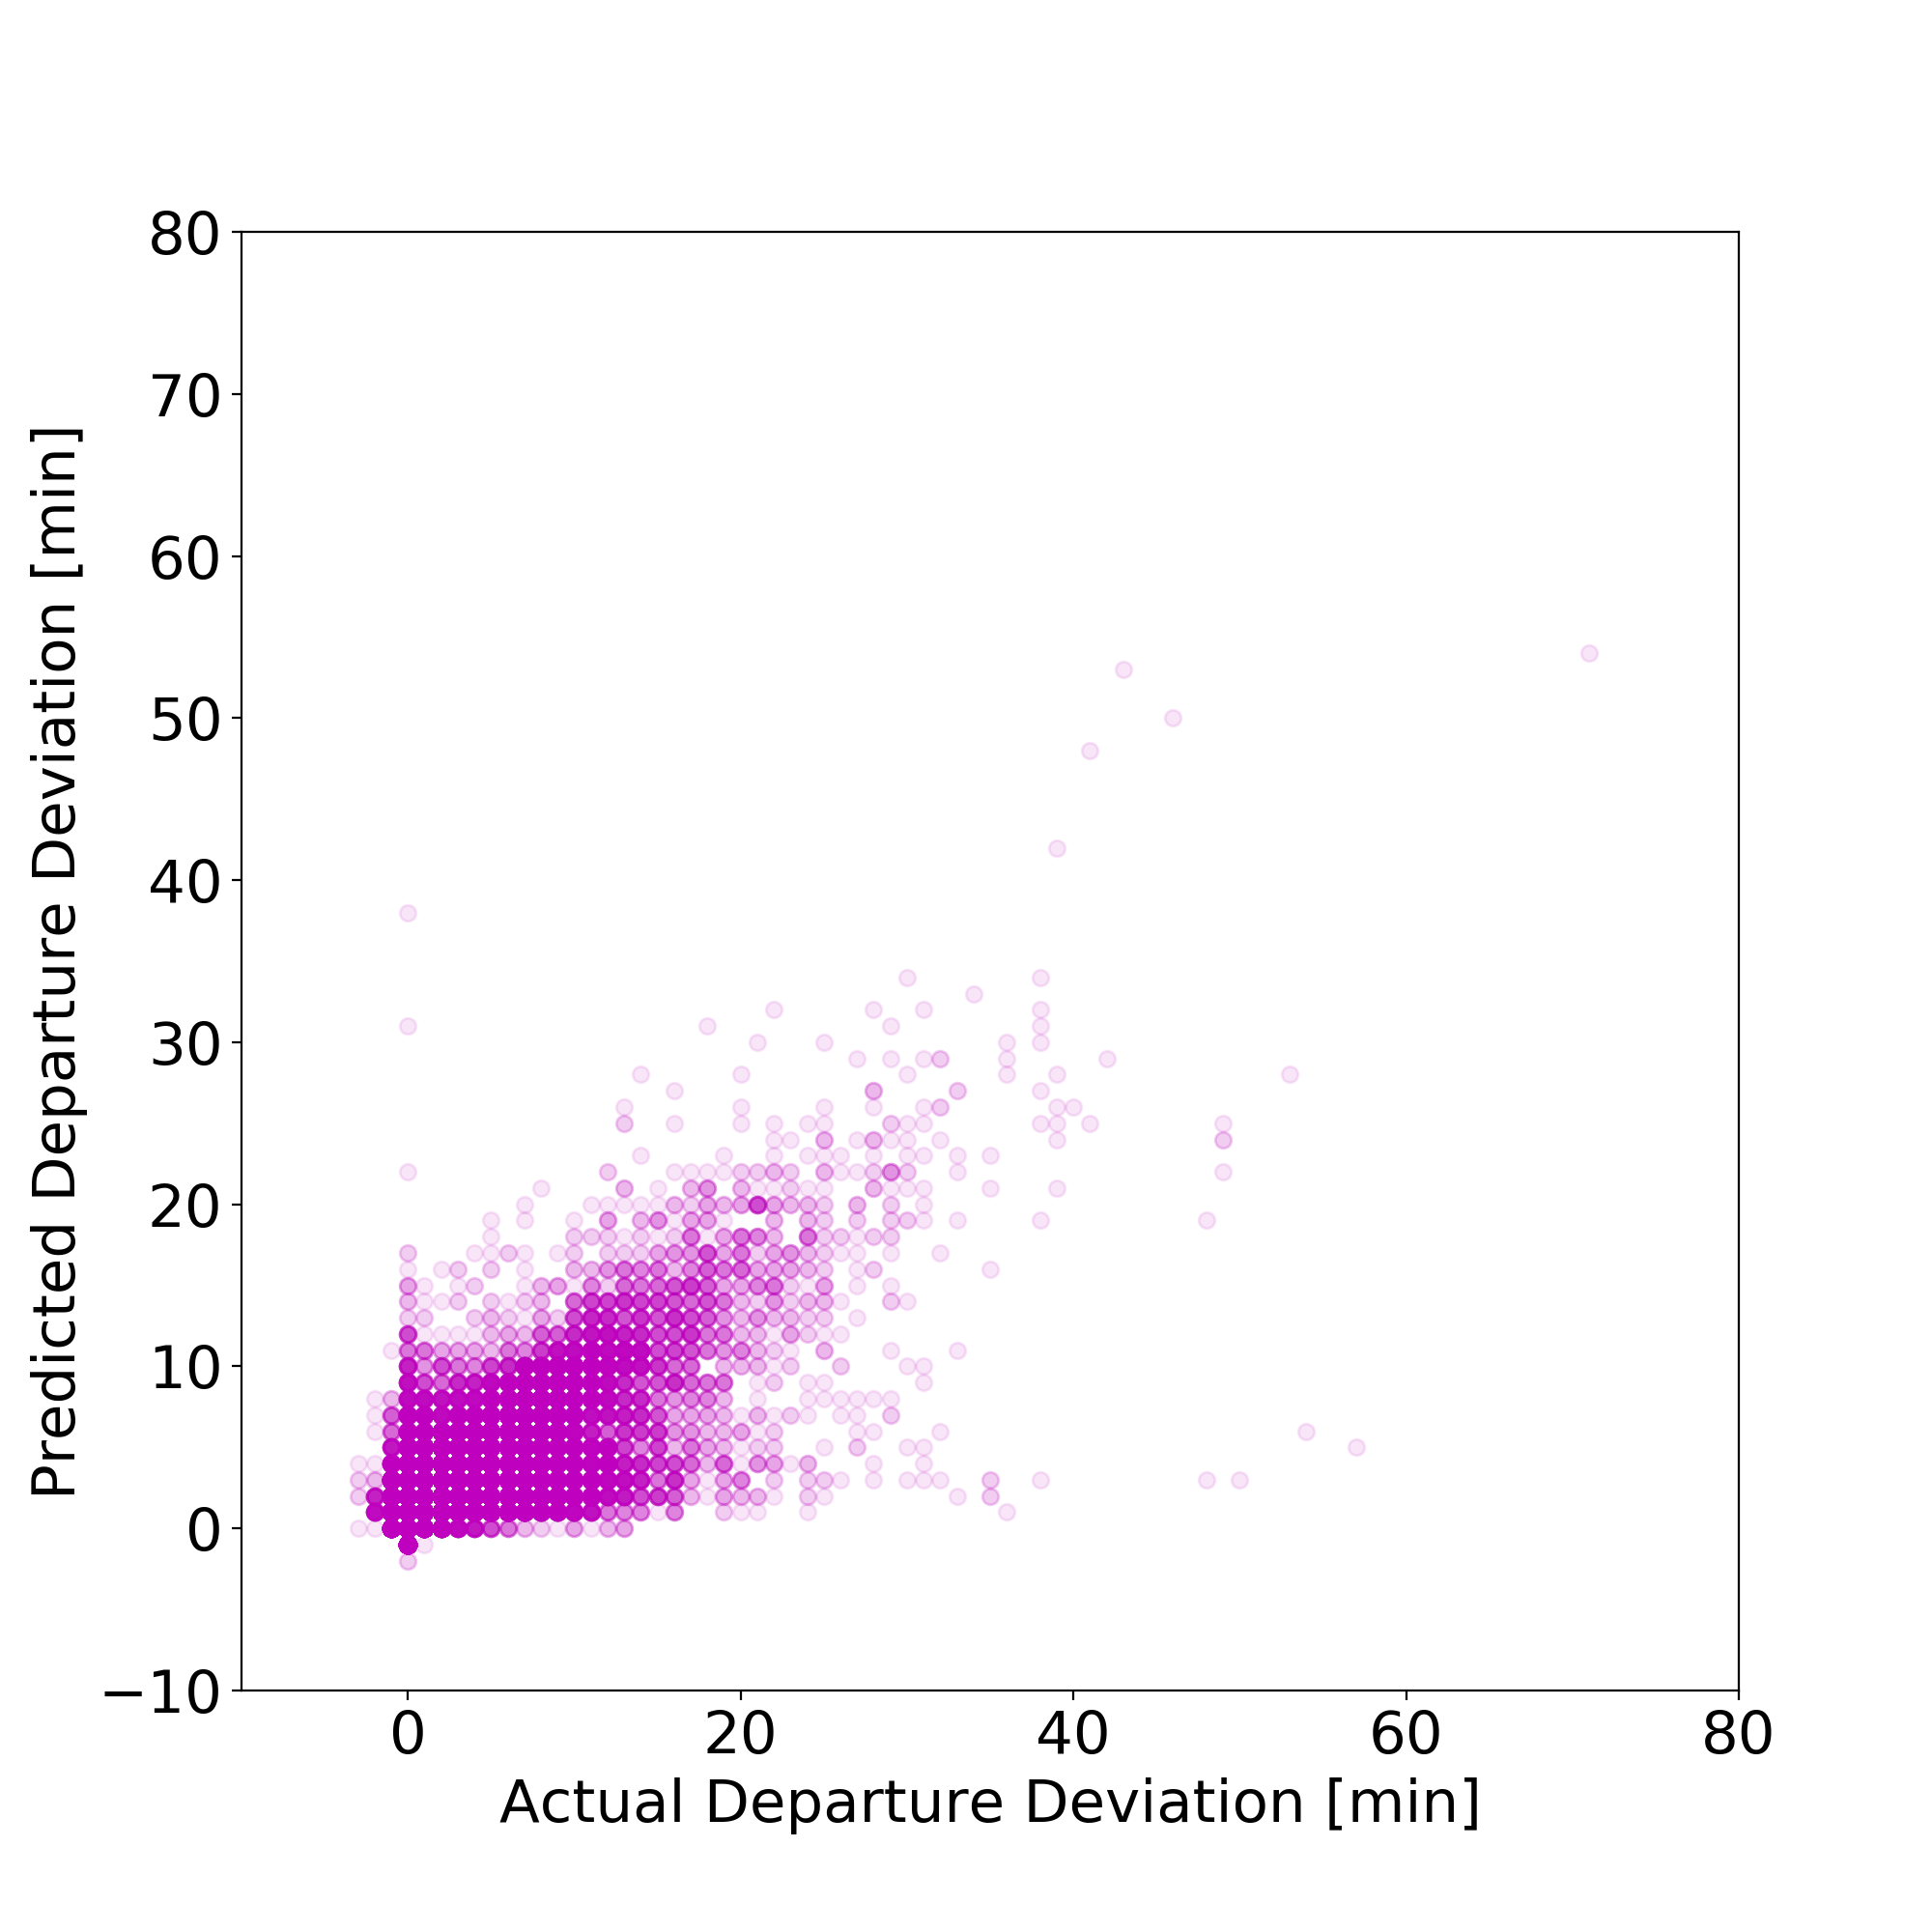
\includegraphics[width=0.5\textwidth]{Images/XGBoost_plot/6_step/6_step_depature_deviation.png}\label{fig:6_step_depature_deviation}}
\end{figure}
\begin{figure}[H]
\centering
\subfloat[\tiny{6-Step DNN Travel Time}]{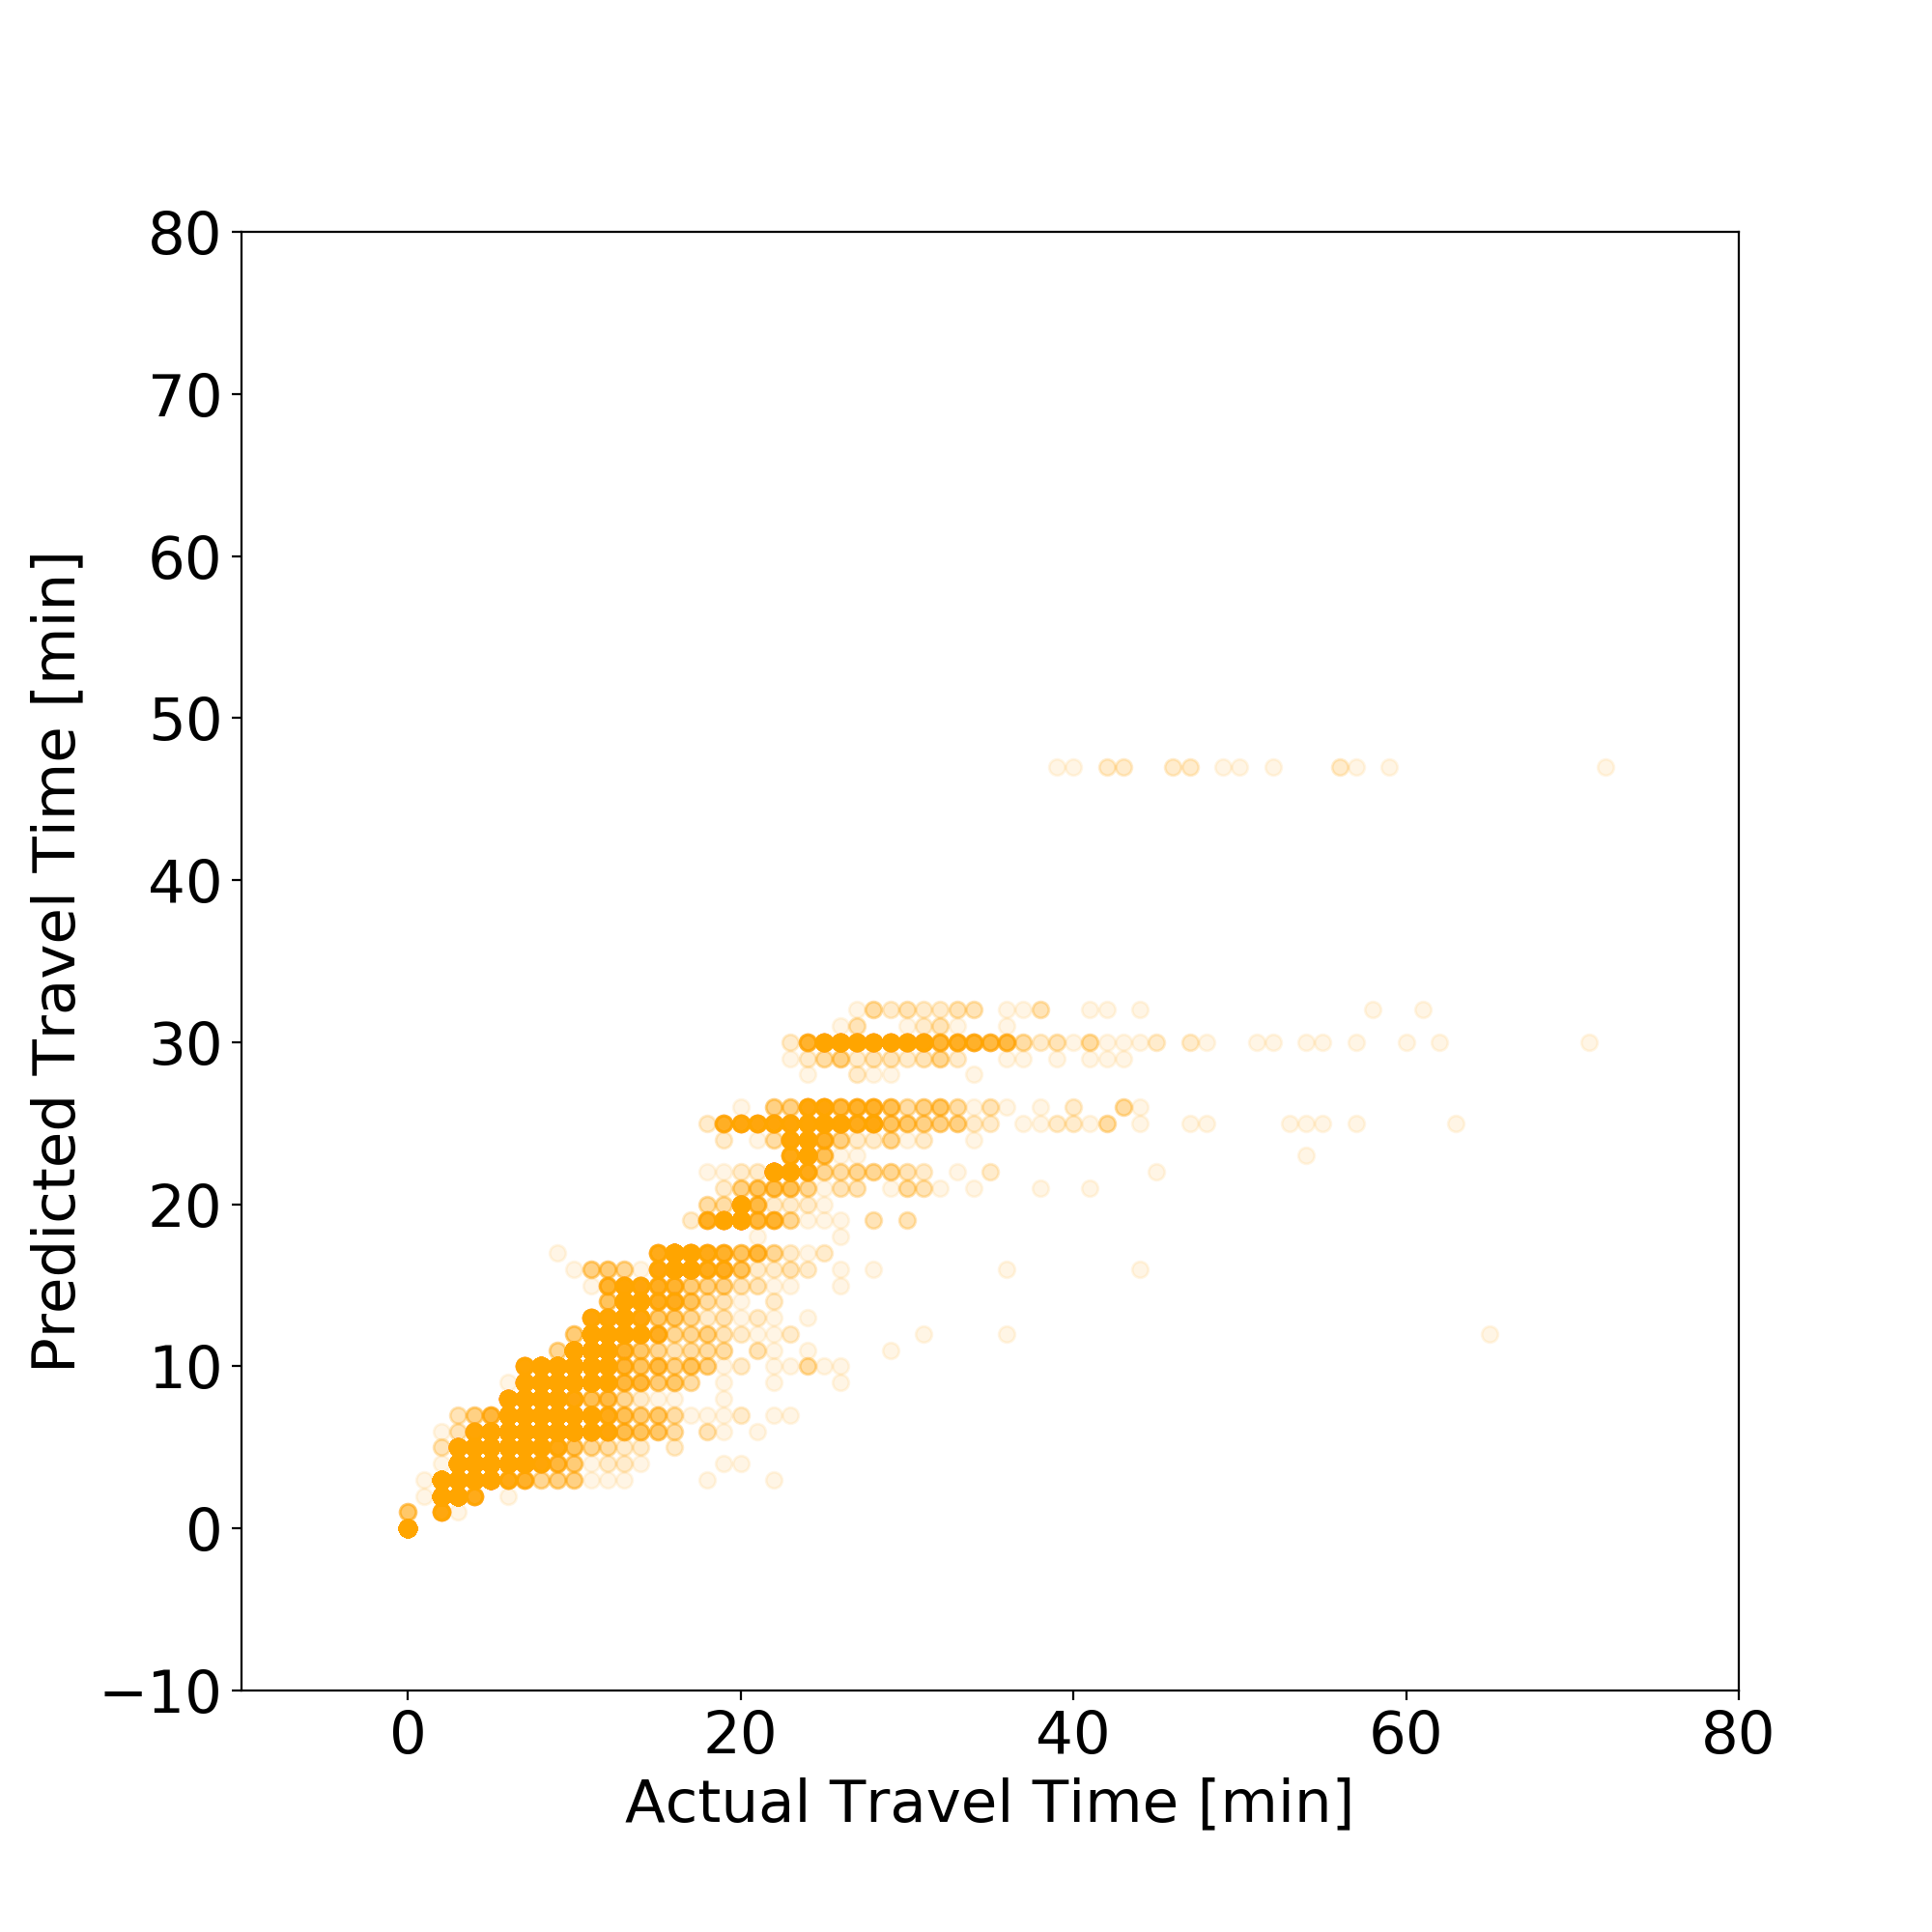
\includegraphics[width=0.5\textwidth]{Images/DNN_plot/6_step/6_step_travel_time.png}\label{fig:6_step_travel_time}}
\subfloat[\tiny{6-Step XGBoost Travel Time}]{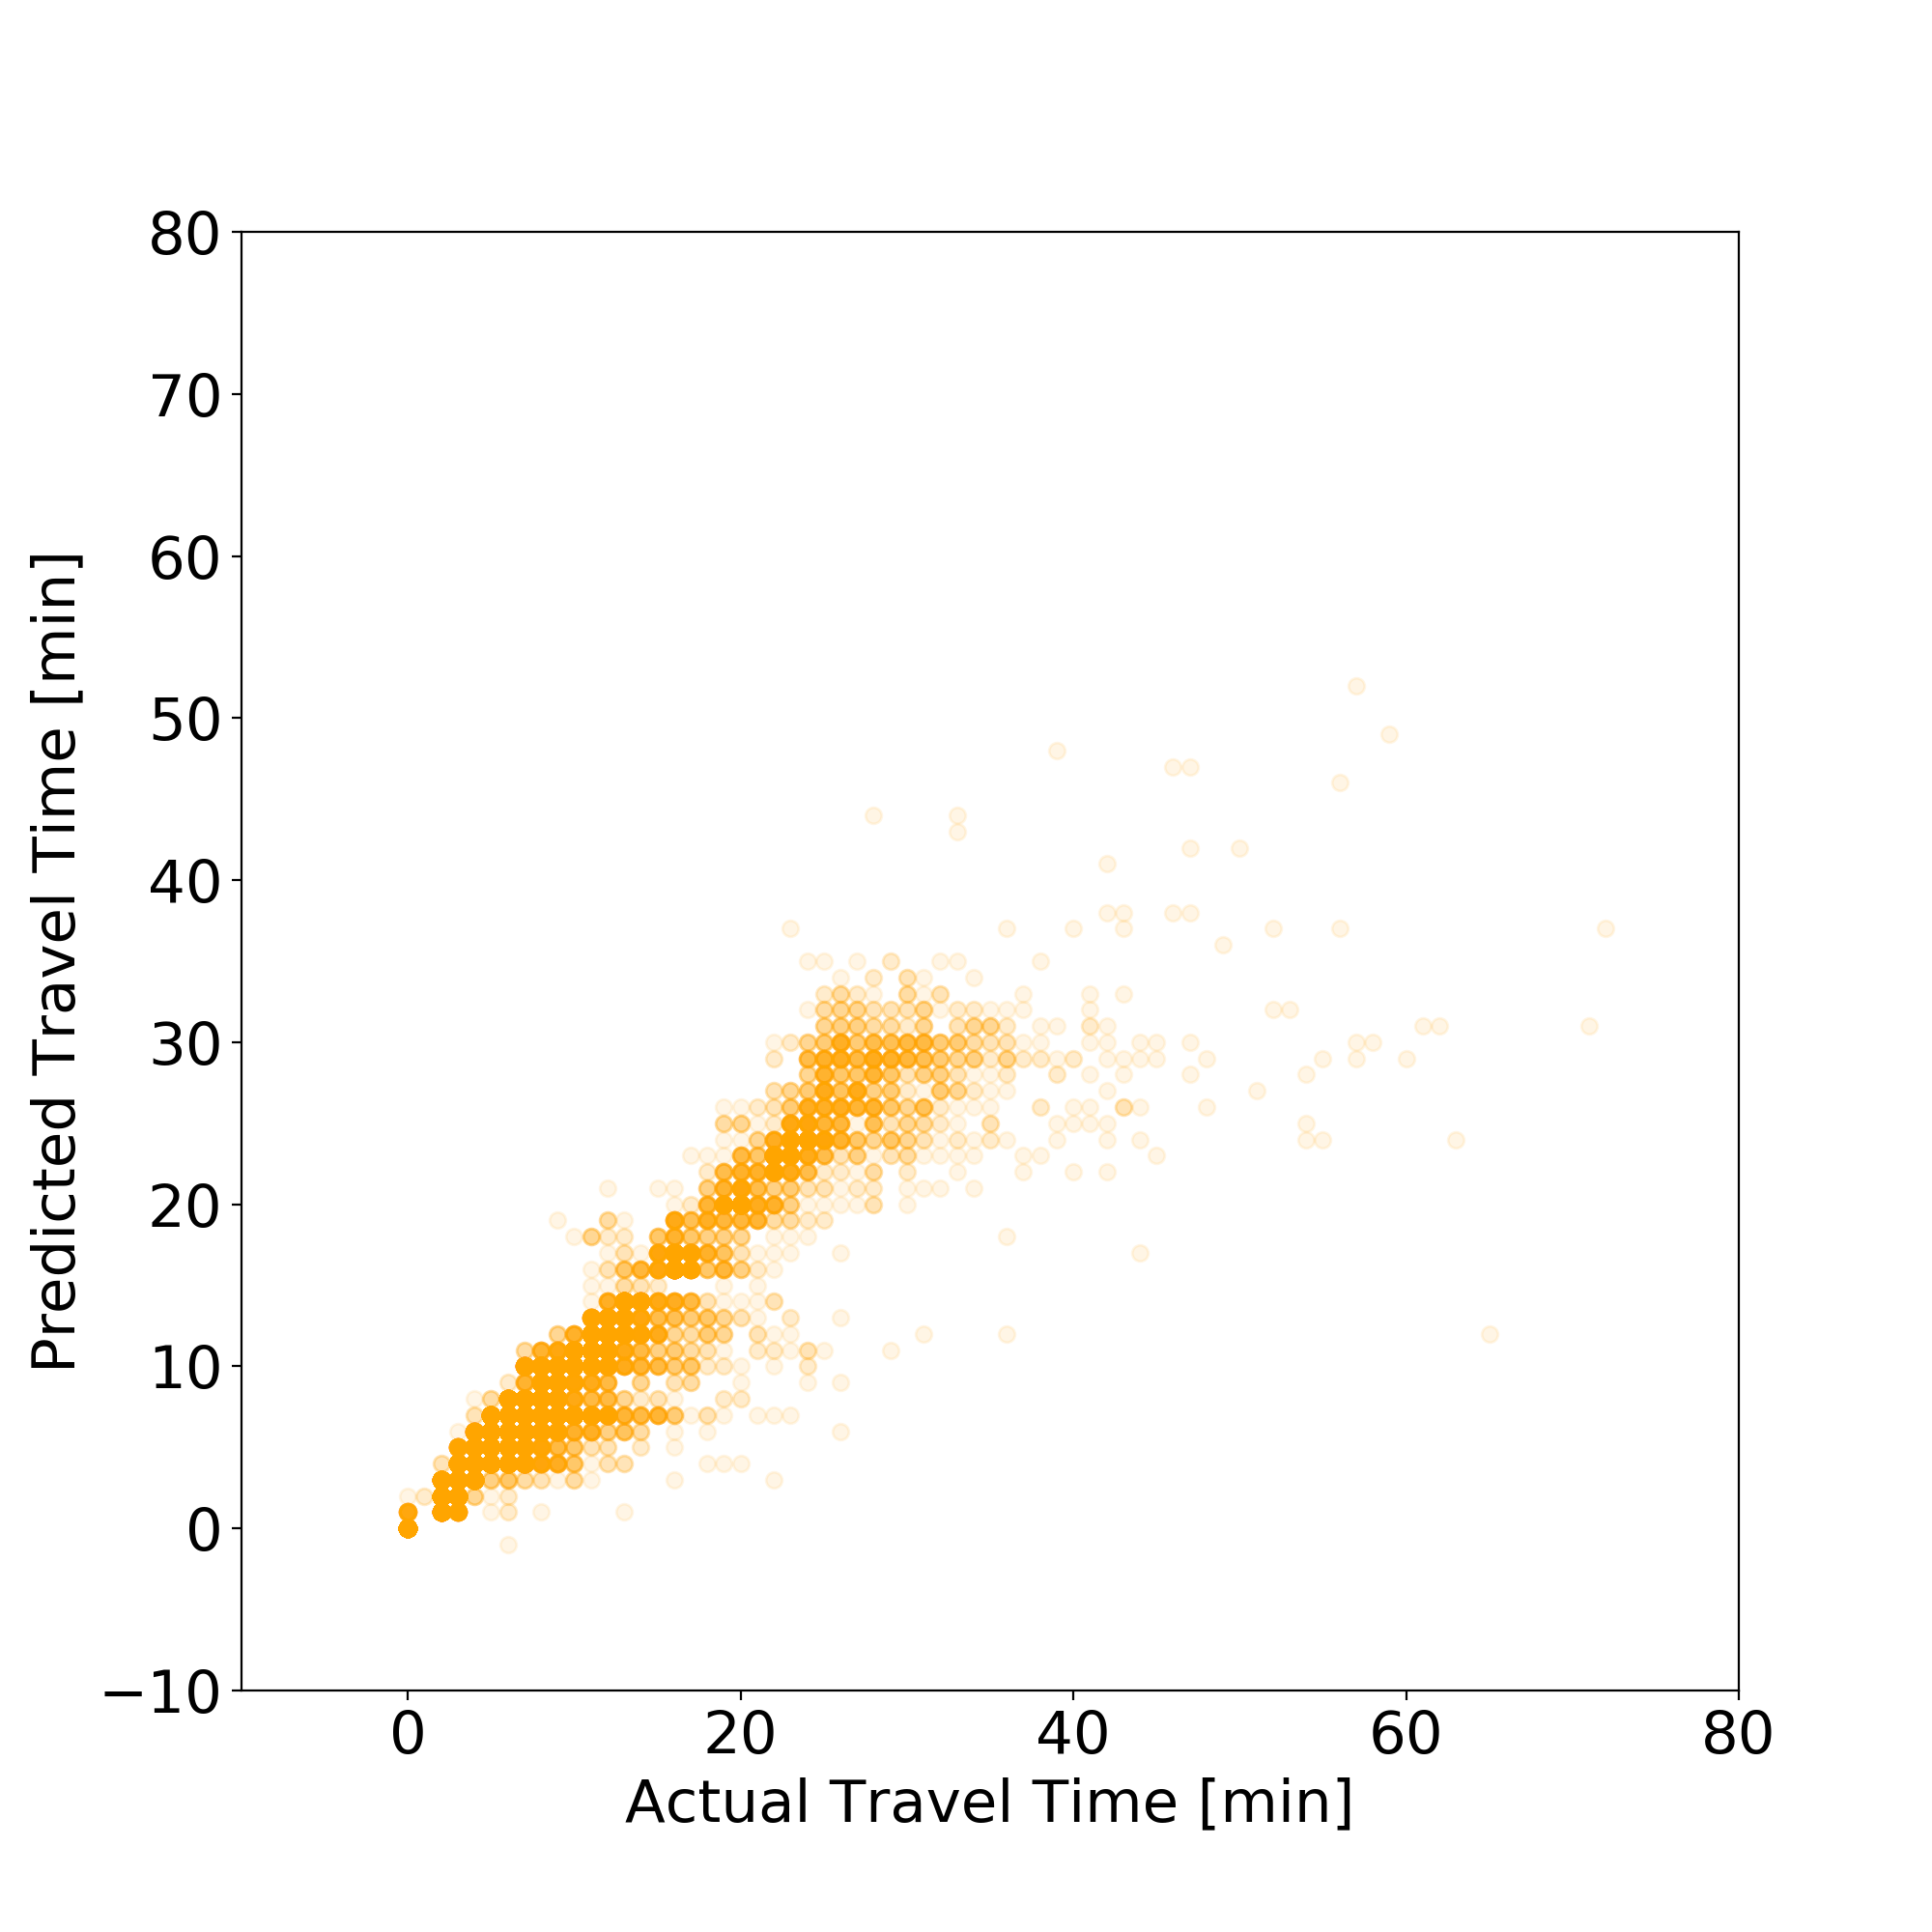
\includegraphics[width=0.5\textwidth]{Images/XGBoost_plot/6_step/6_step_travel_time.png}\label{fig:6_step_travel_time}}
\end{figure}
\begin{figure}[H]
\centering
\subfloat[\tiny{6-Step DNN Dwell Time}]{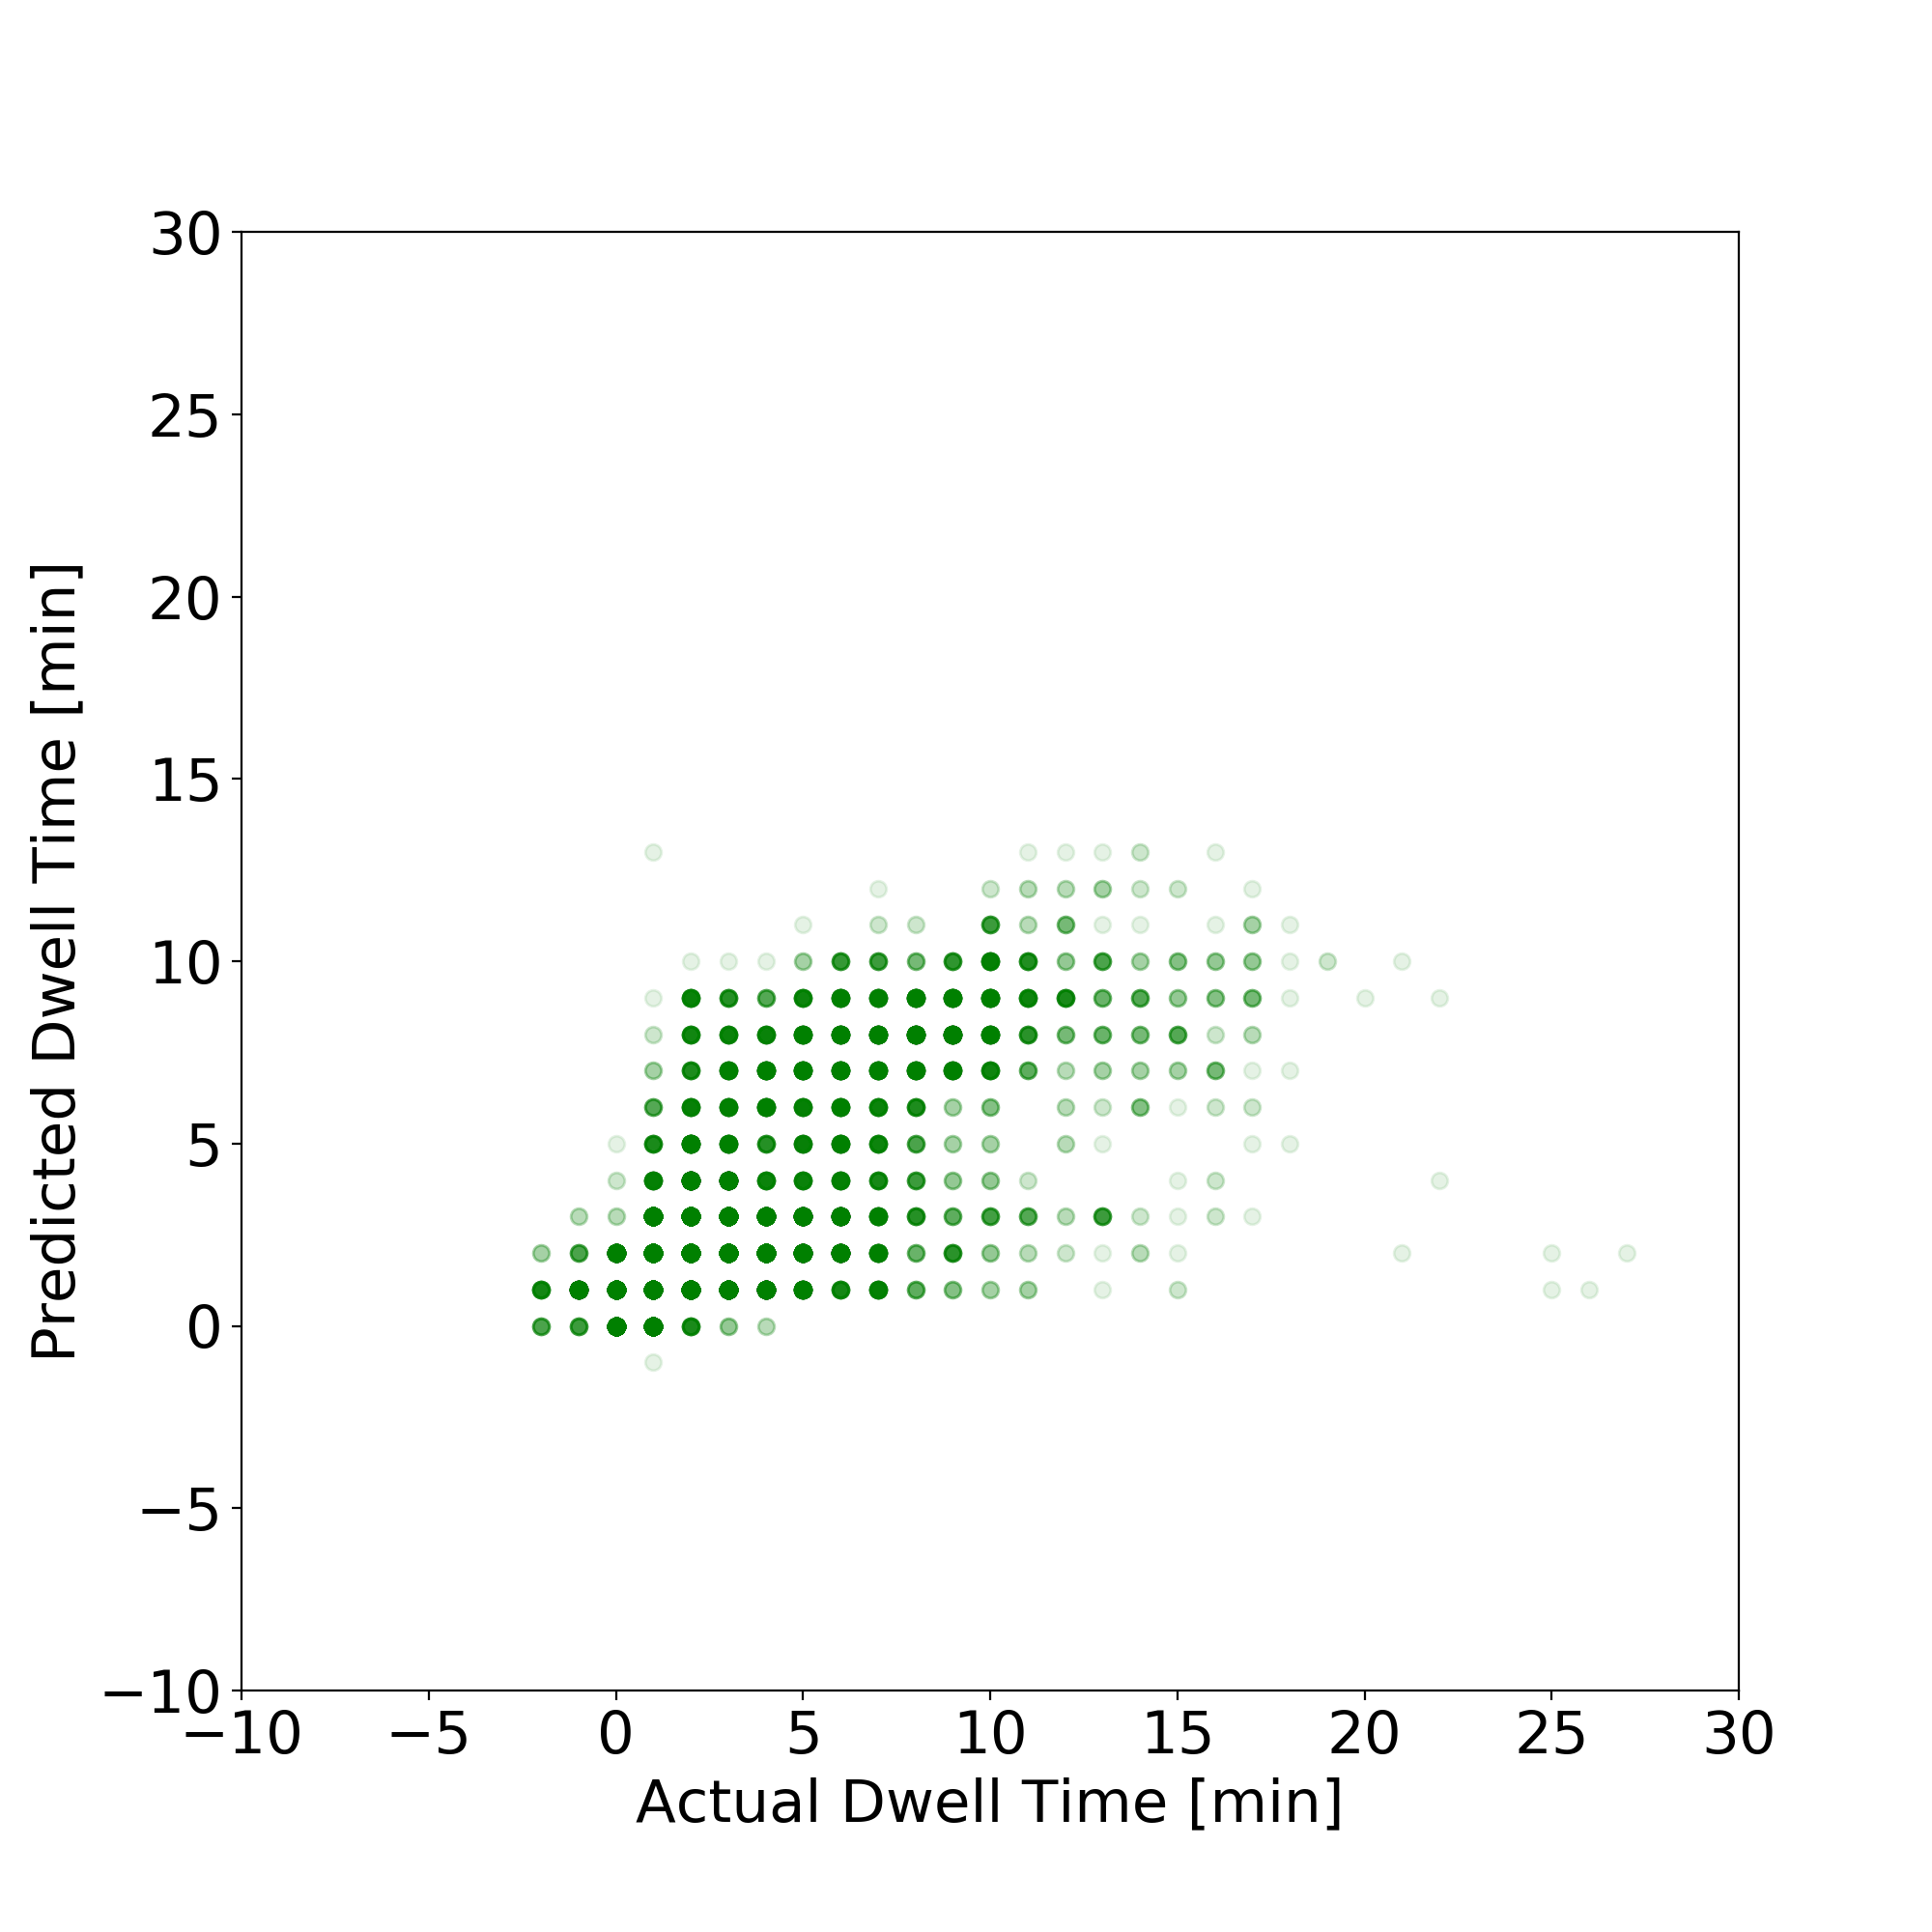
\includegraphics[width=0.5\textwidth]{Images/DNN_plot/6_step/6_step_dwell_time.png}\label{fig:6_step_dwell_time}}
\subfloat[\tiny{6-Step XGBoost Dwell Time}]{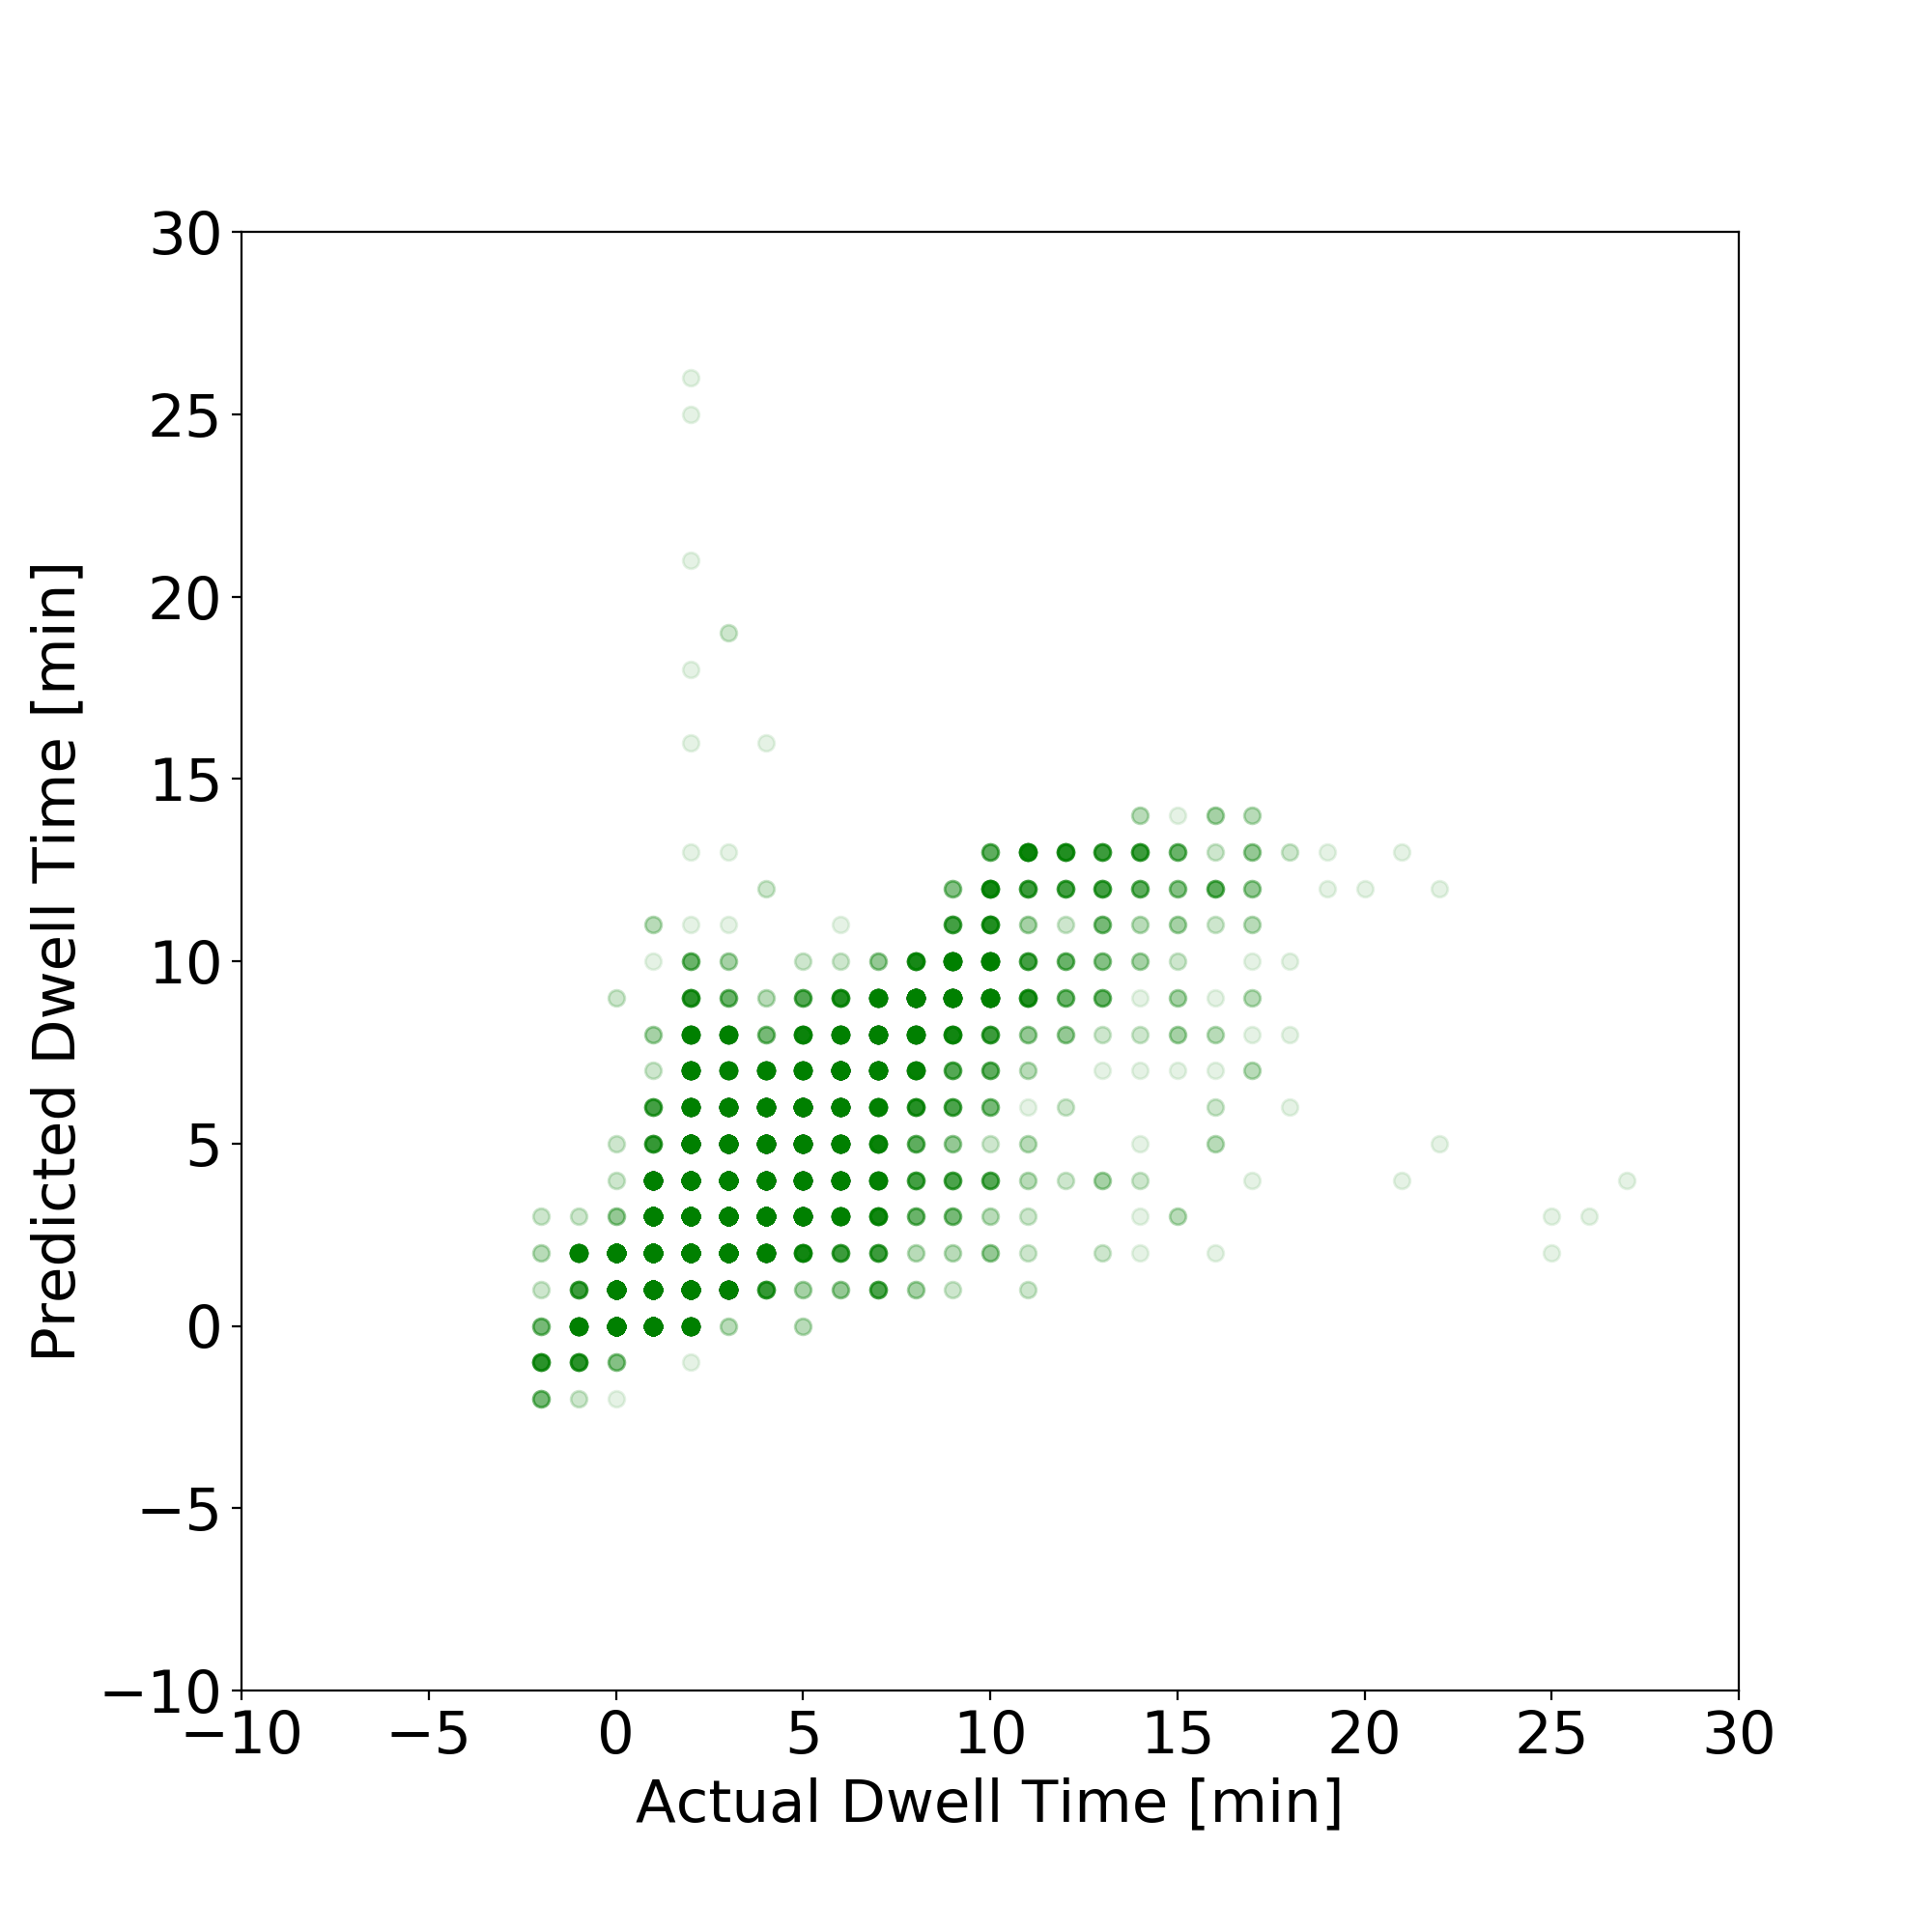
\includegraphics[width=0.5\textwidth]{Images/XGBoost_plot/6_step/6_step_dwell_time.png}\label{fig:6_step_dwell_time}}
\end{figure}

\begin{figure}[H]
\centering
\subfloat[\tiny{7-Step DNN Deviation from Arrival}]{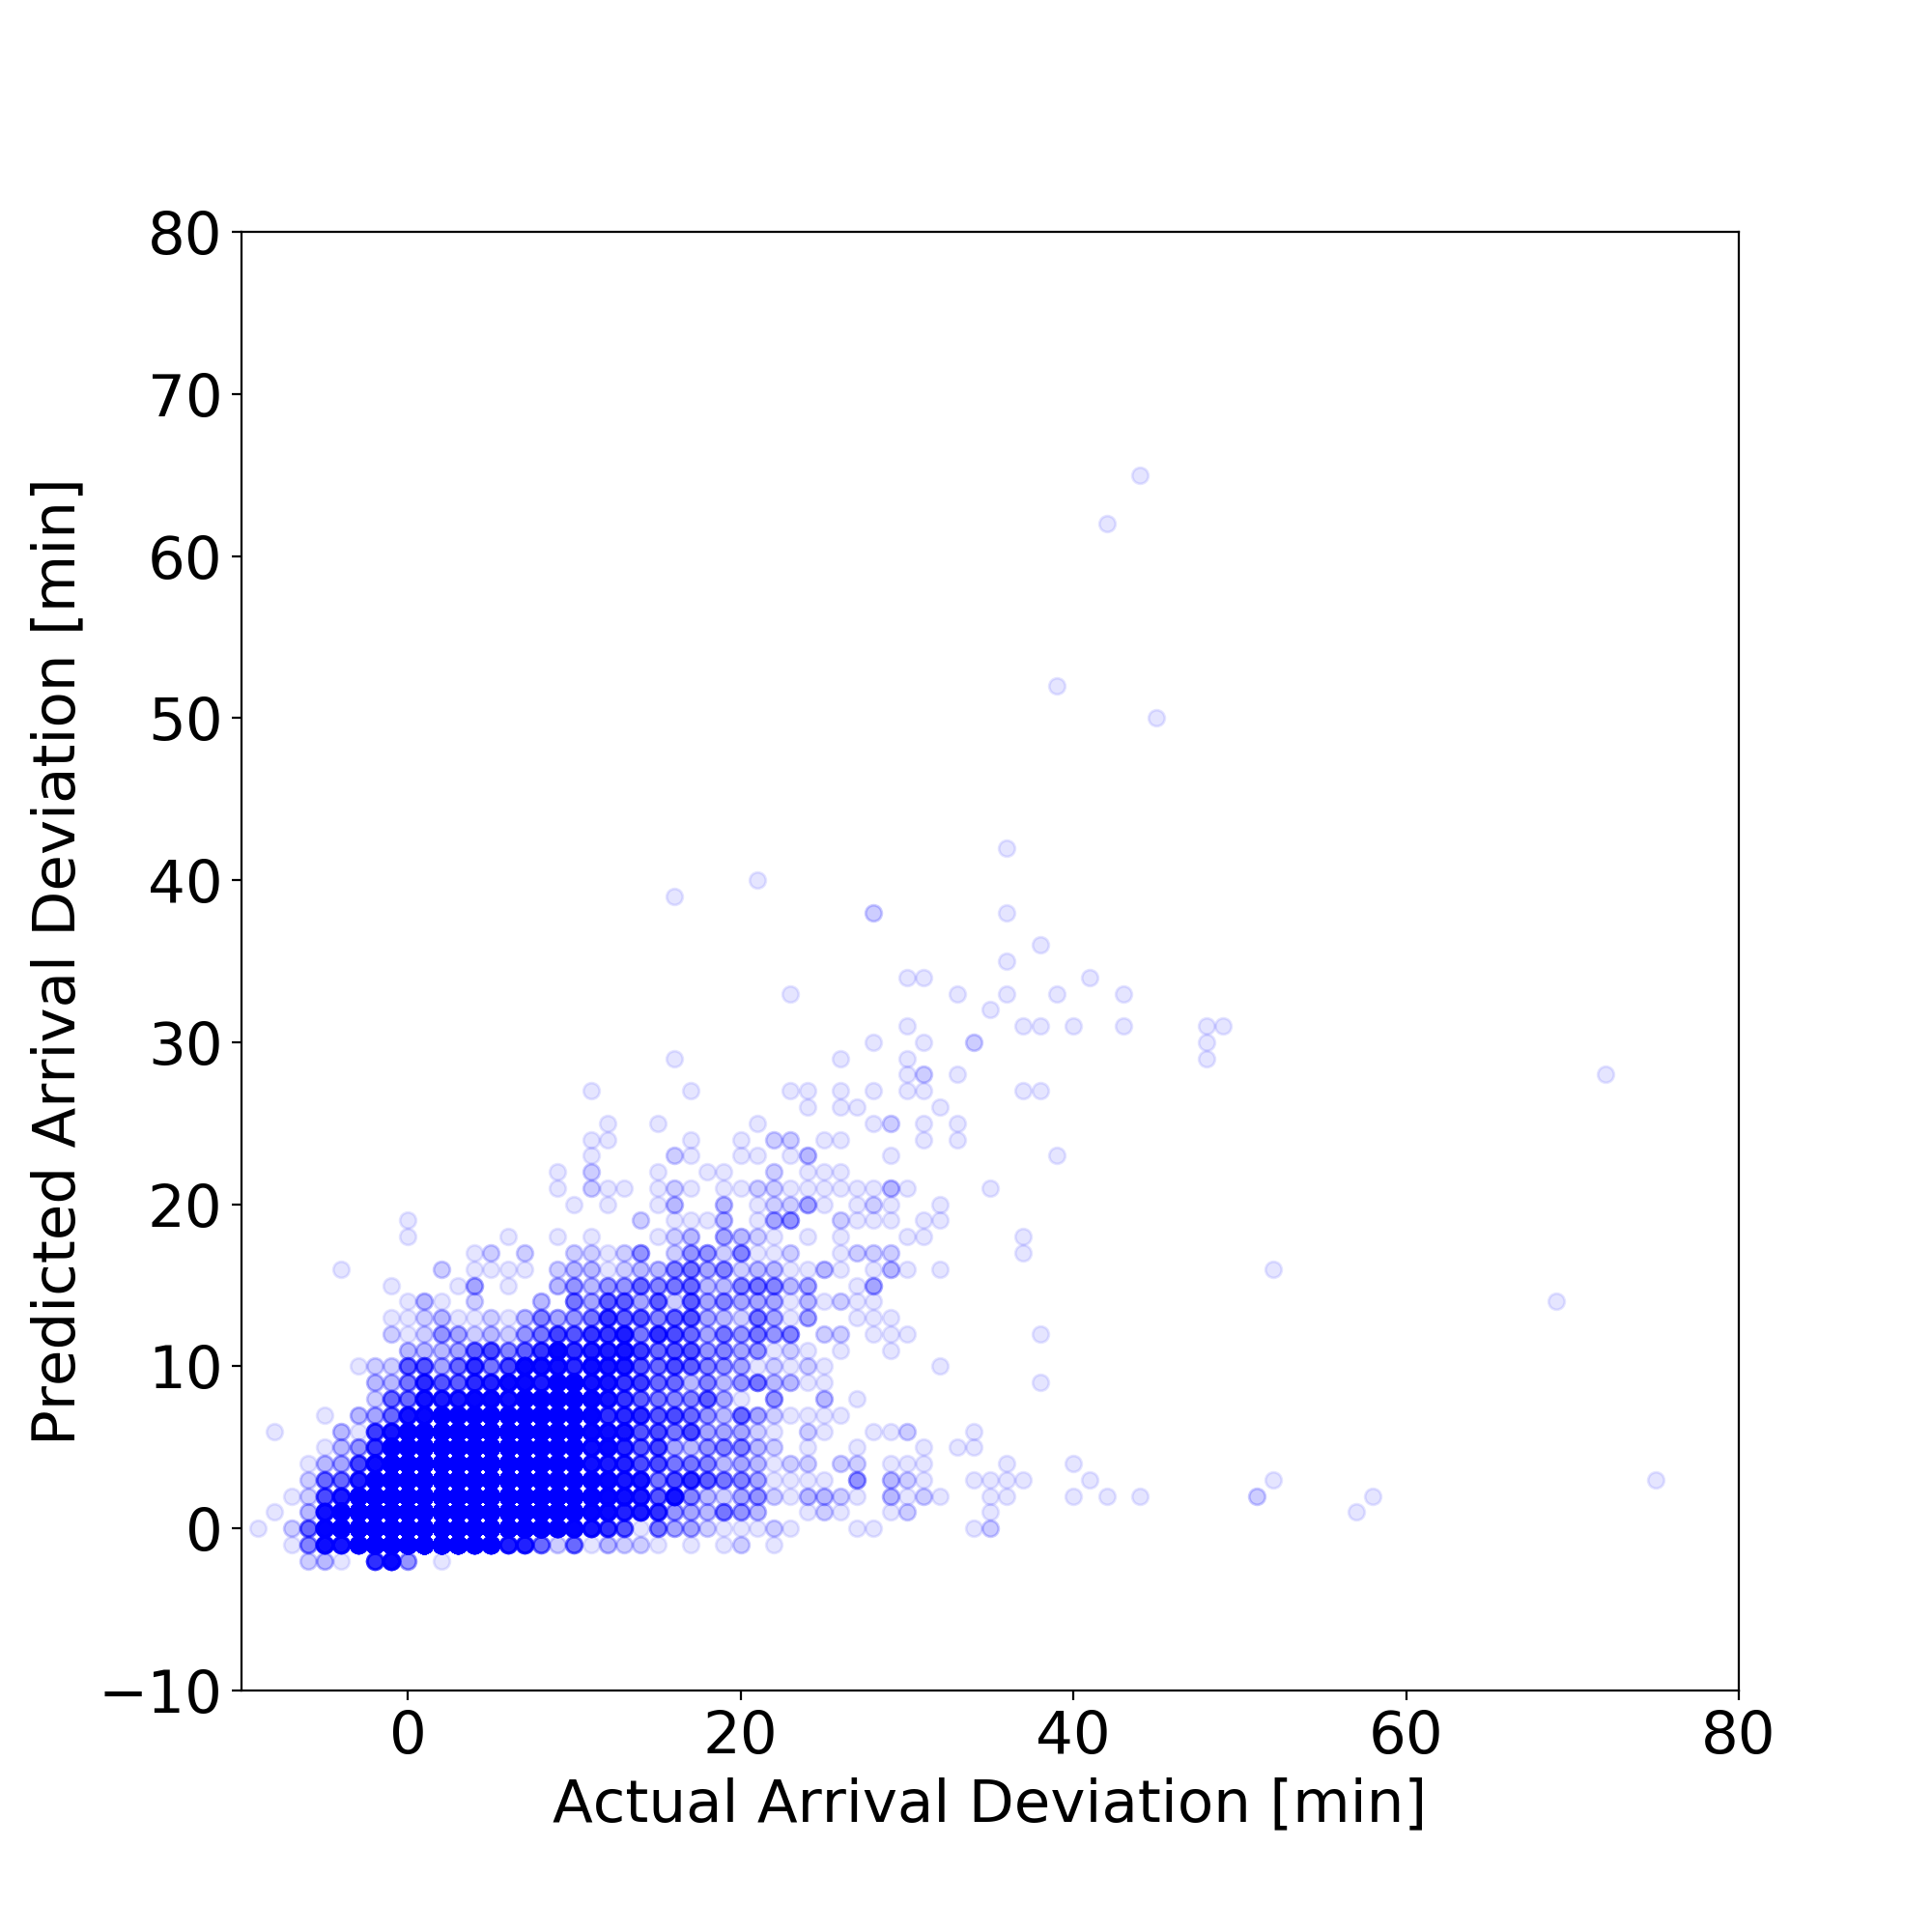
\includegraphics[width=0.5\textwidth]{Images/DNN_plot/7_step/7_step_arrival_deviation.png}\label{fig:7_step_arrival_deviation}}
\subfloat[\tiny{7-Step XGBoost Deviation from Arrival}]{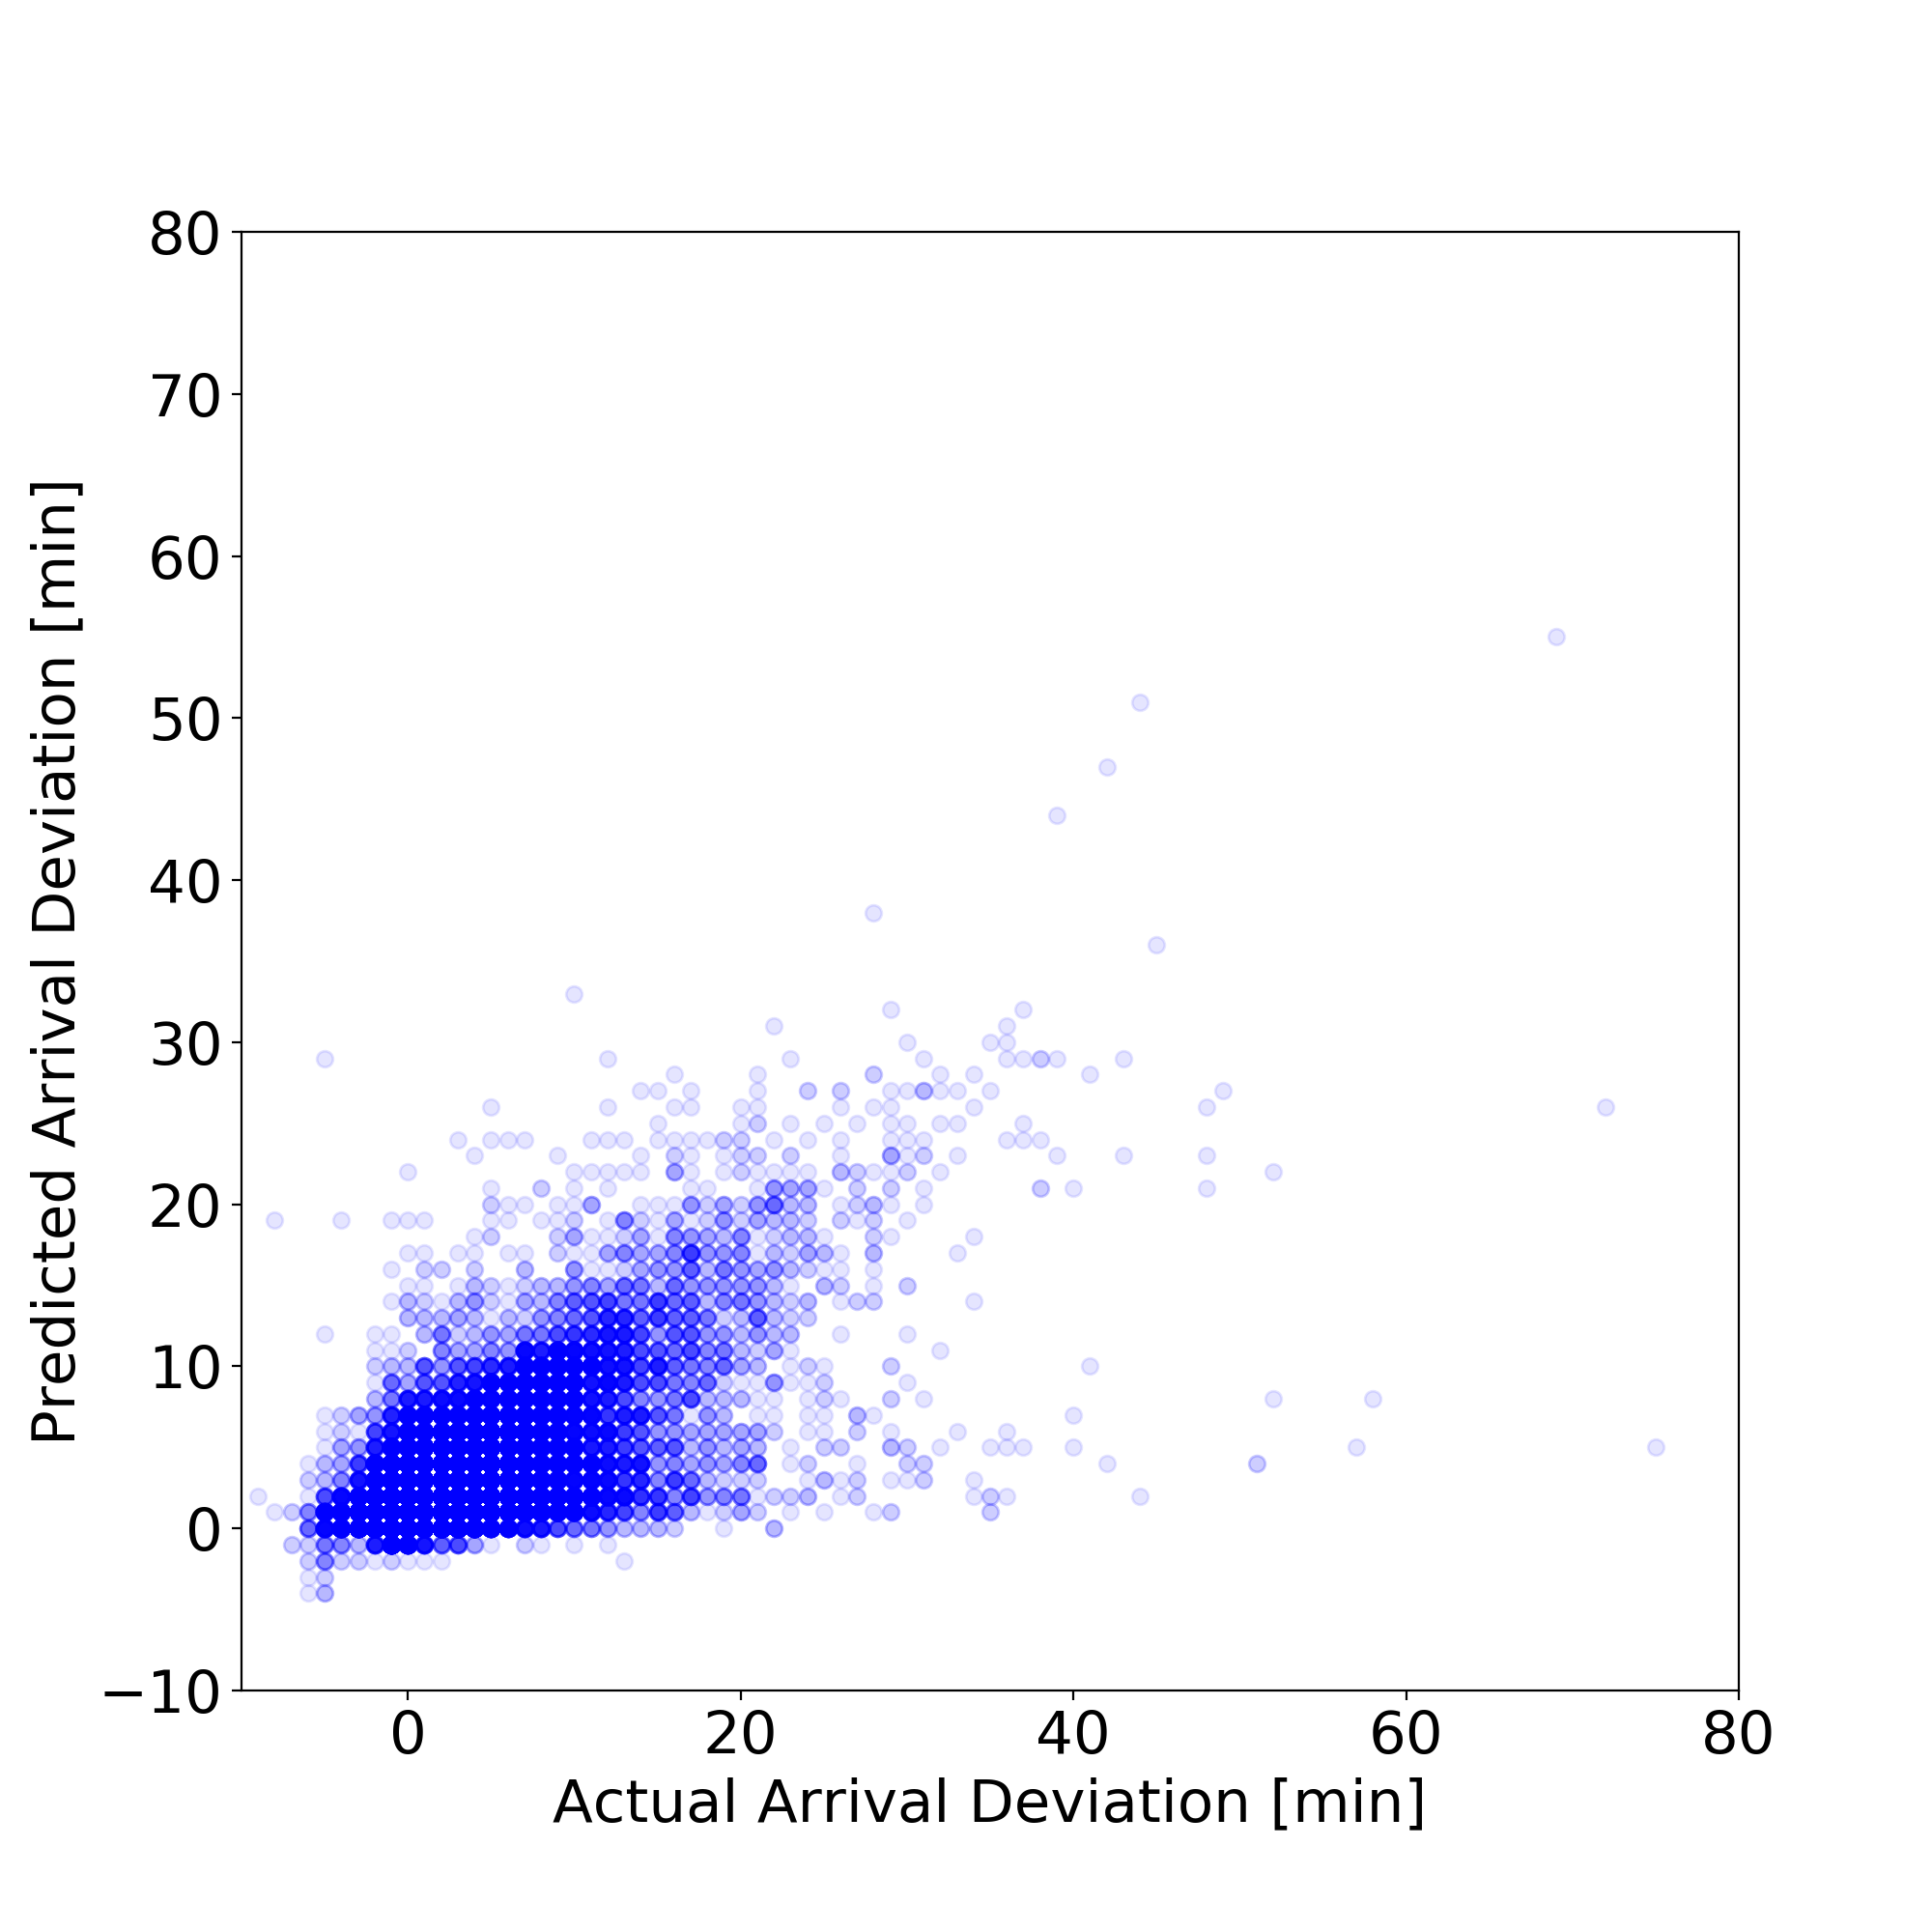
\includegraphics[width=0.5\textwidth]{Images/XGBoost_plot/7_step/7_step_arrival_deviation.png}\label{fig:7_step_arrival_deviation}}
\end{figure}
\begin{figure}[H]
\centering
\subfloat[\tiny{7-Step DNN Deviation from Departure}]{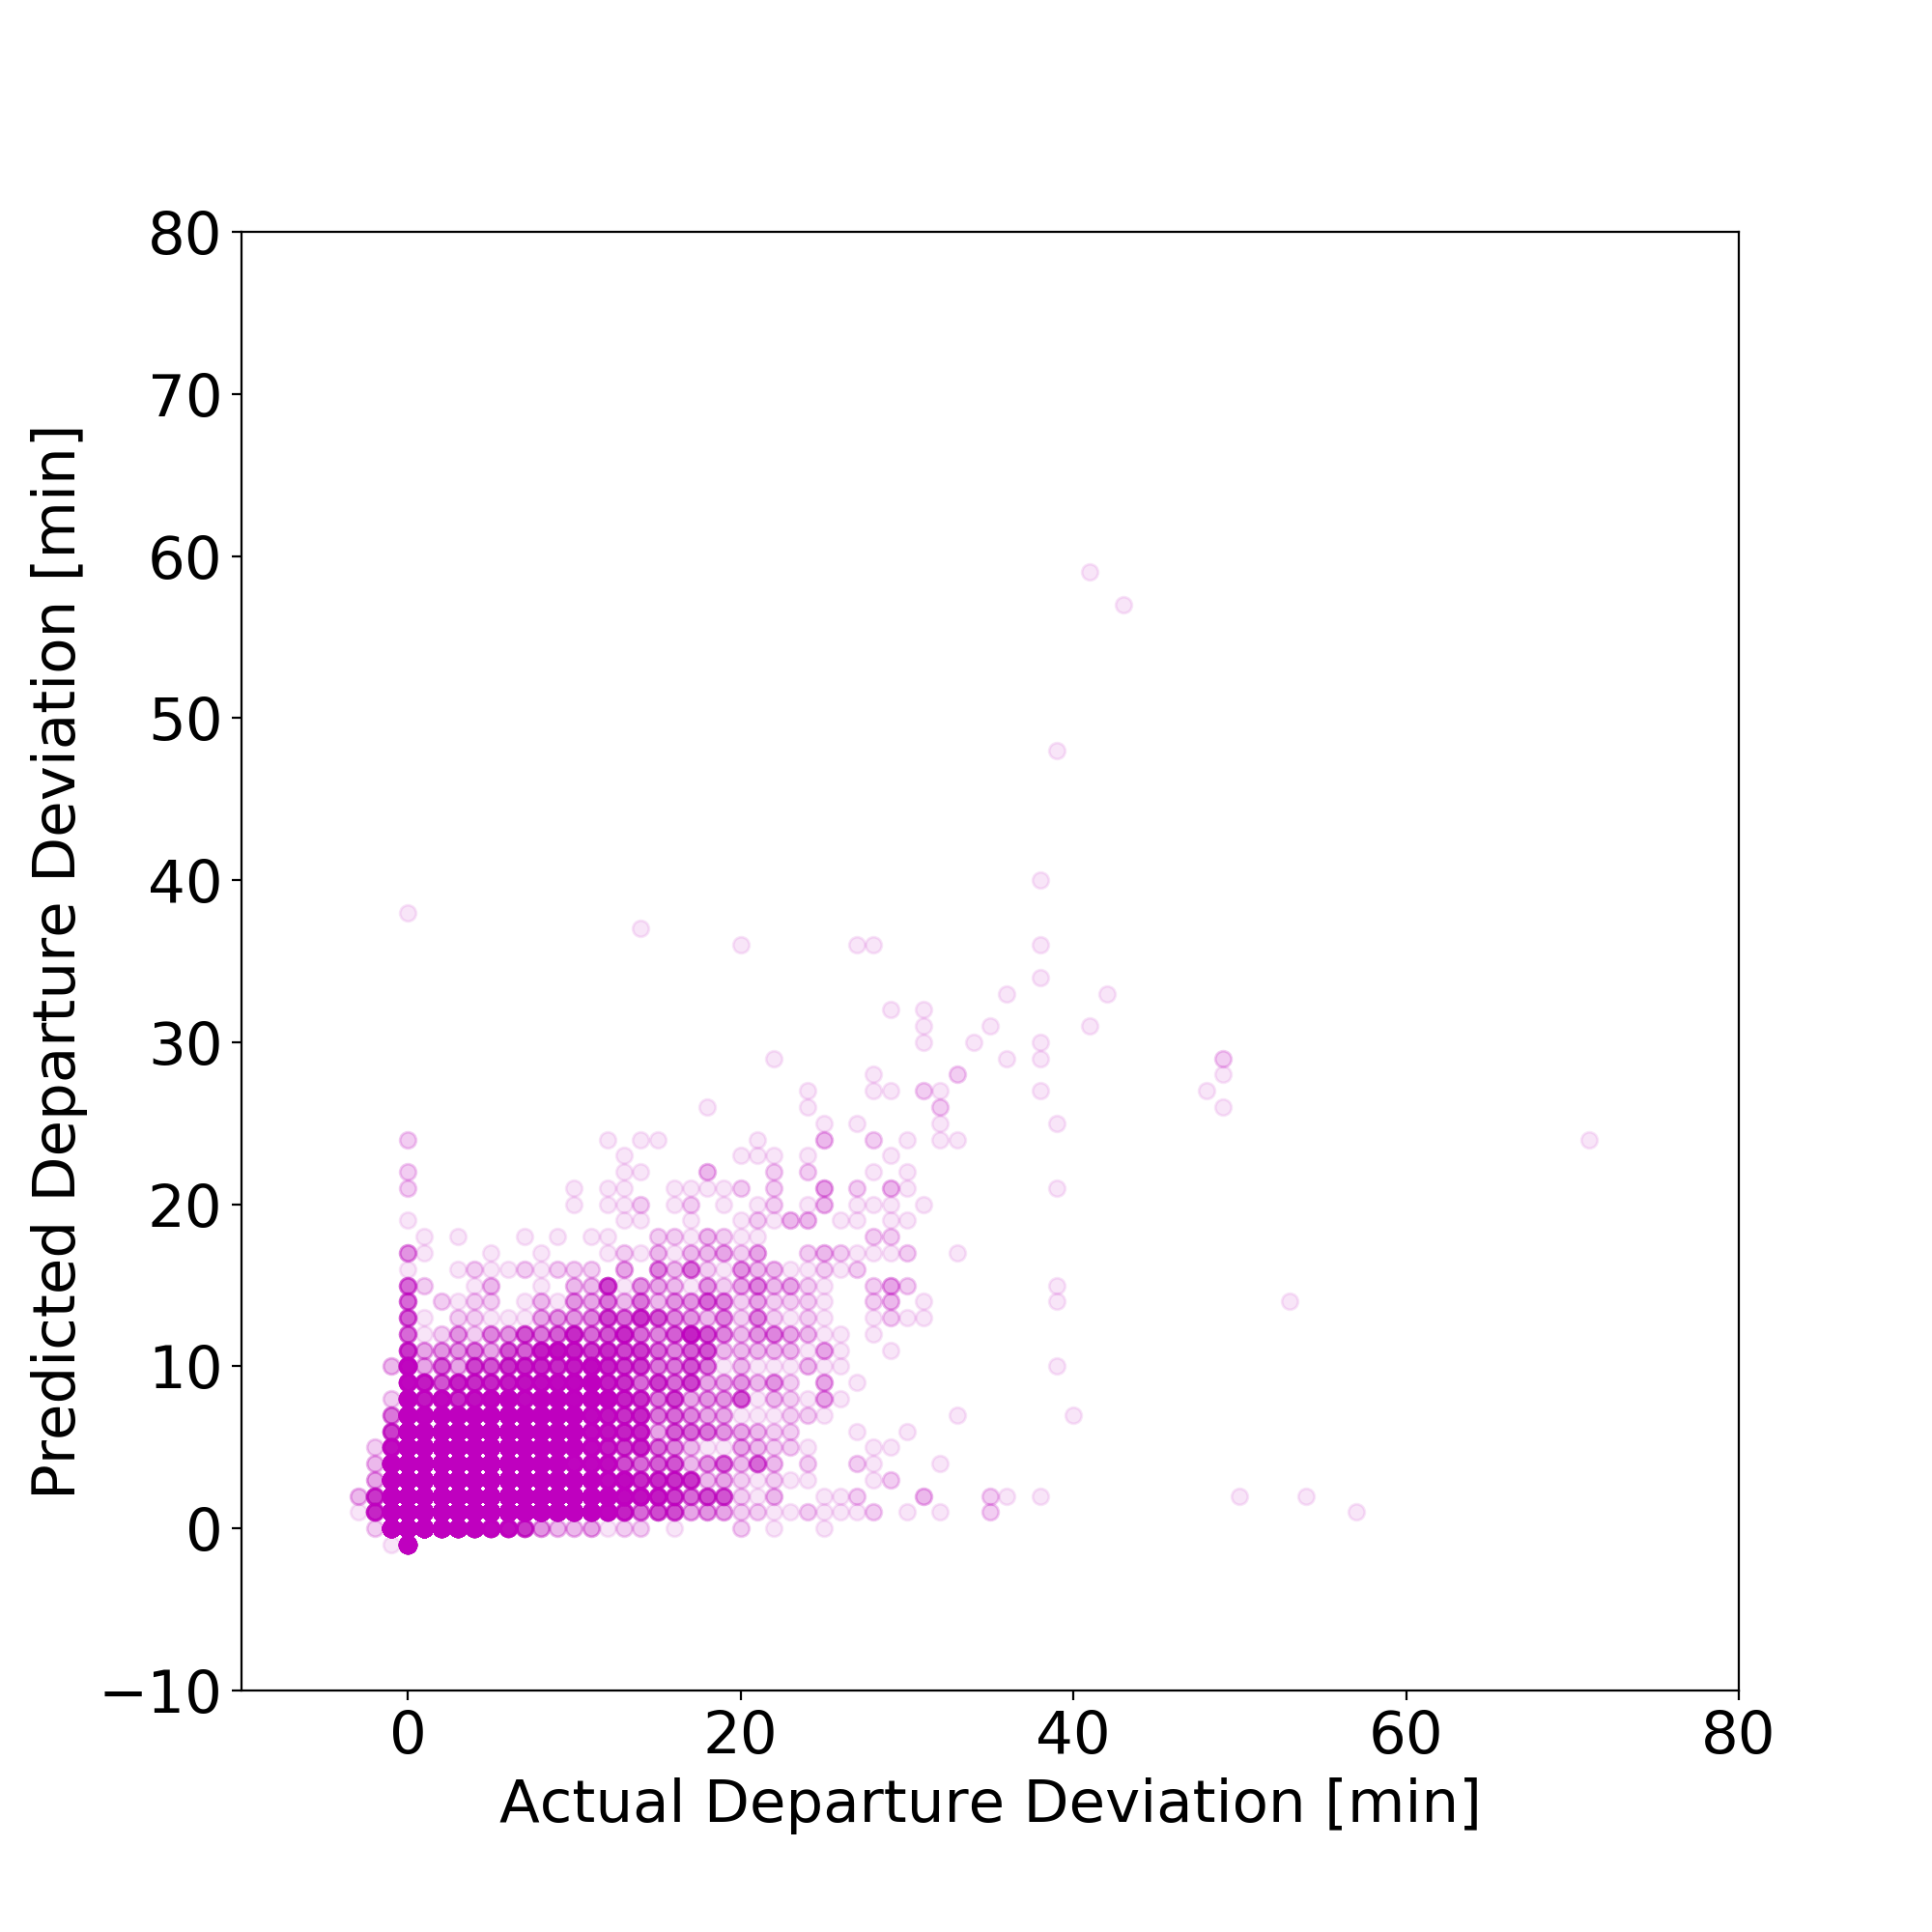
\includegraphics[width=0.5\textwidth]{Images/DNN_plot/7_step/7_step_depature_deviation.png}\label{fig:7_step_depature_deviation}}
\subfloat[\tiny{7-Step XGBoost Deviation from Departure}]{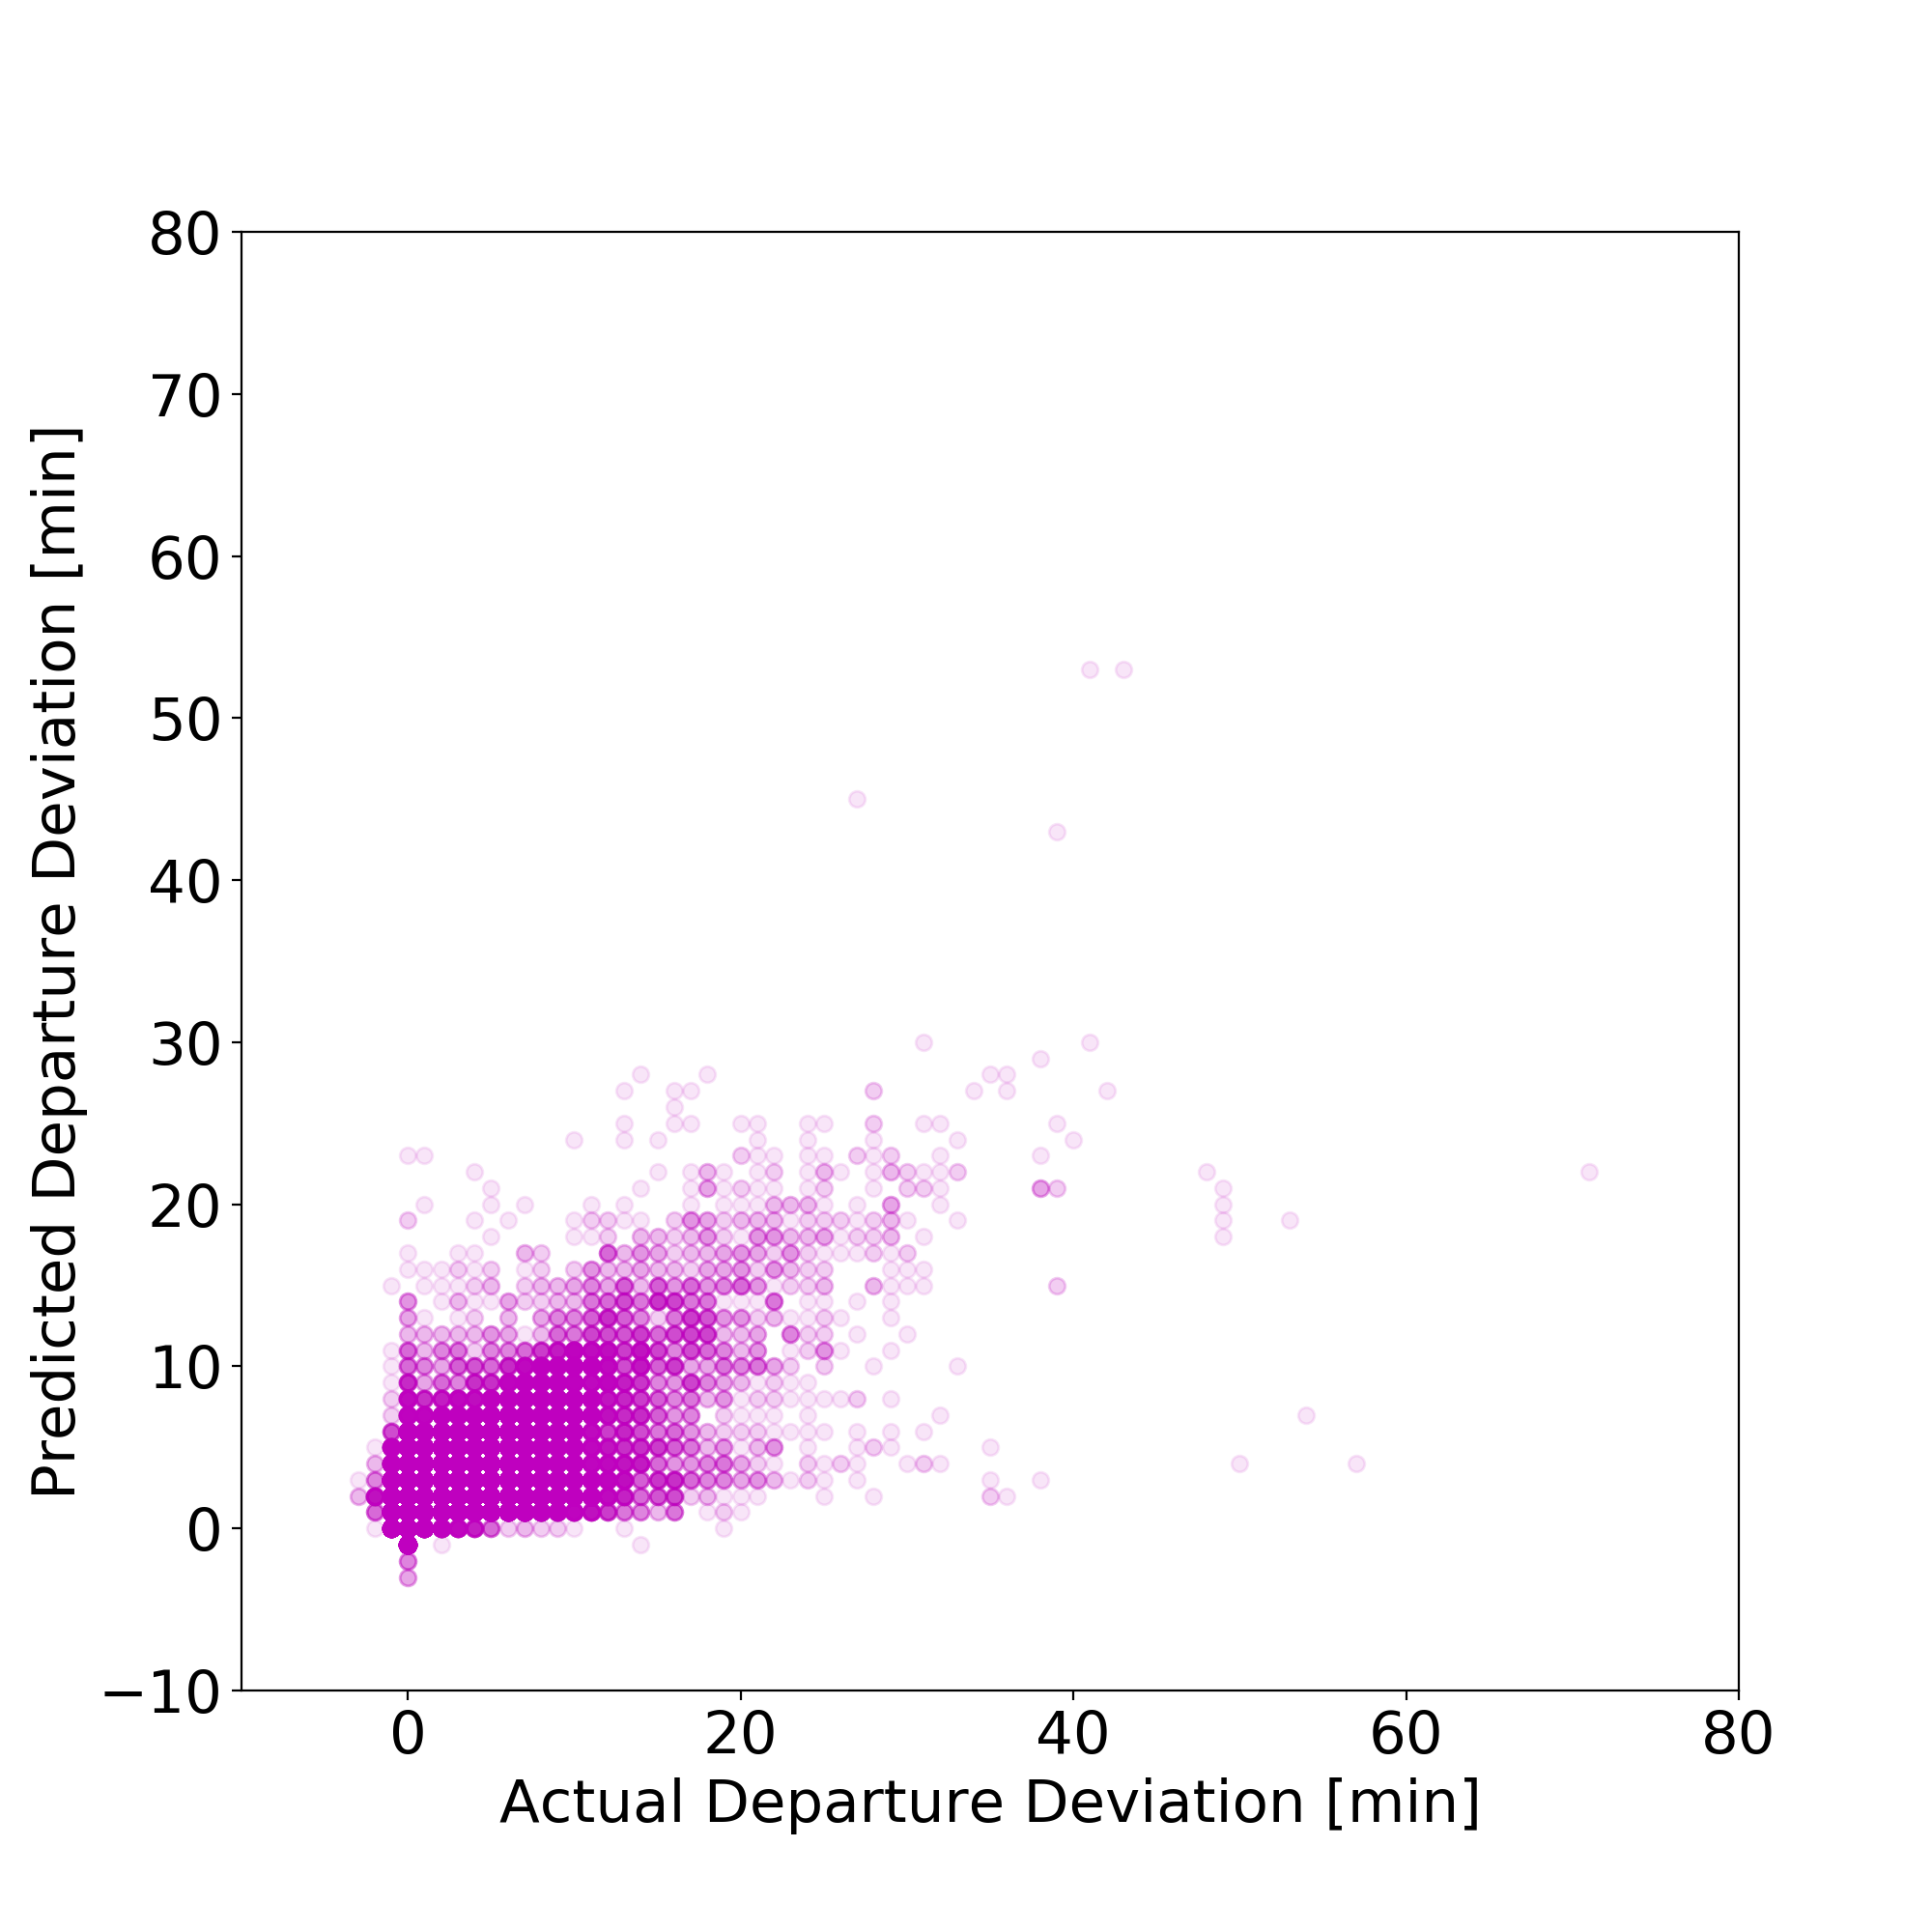
\includegraphics[width=0.5\textwidth]{Images/XGBoost_plot/7_step/7_step_depature_deviation.png}\label{fig:7_step_depature_deviation}}
\end{figure}
\begin{figure}[H]
\centering
\subfloat[\tiny{7-Step DNN Travel Time}]{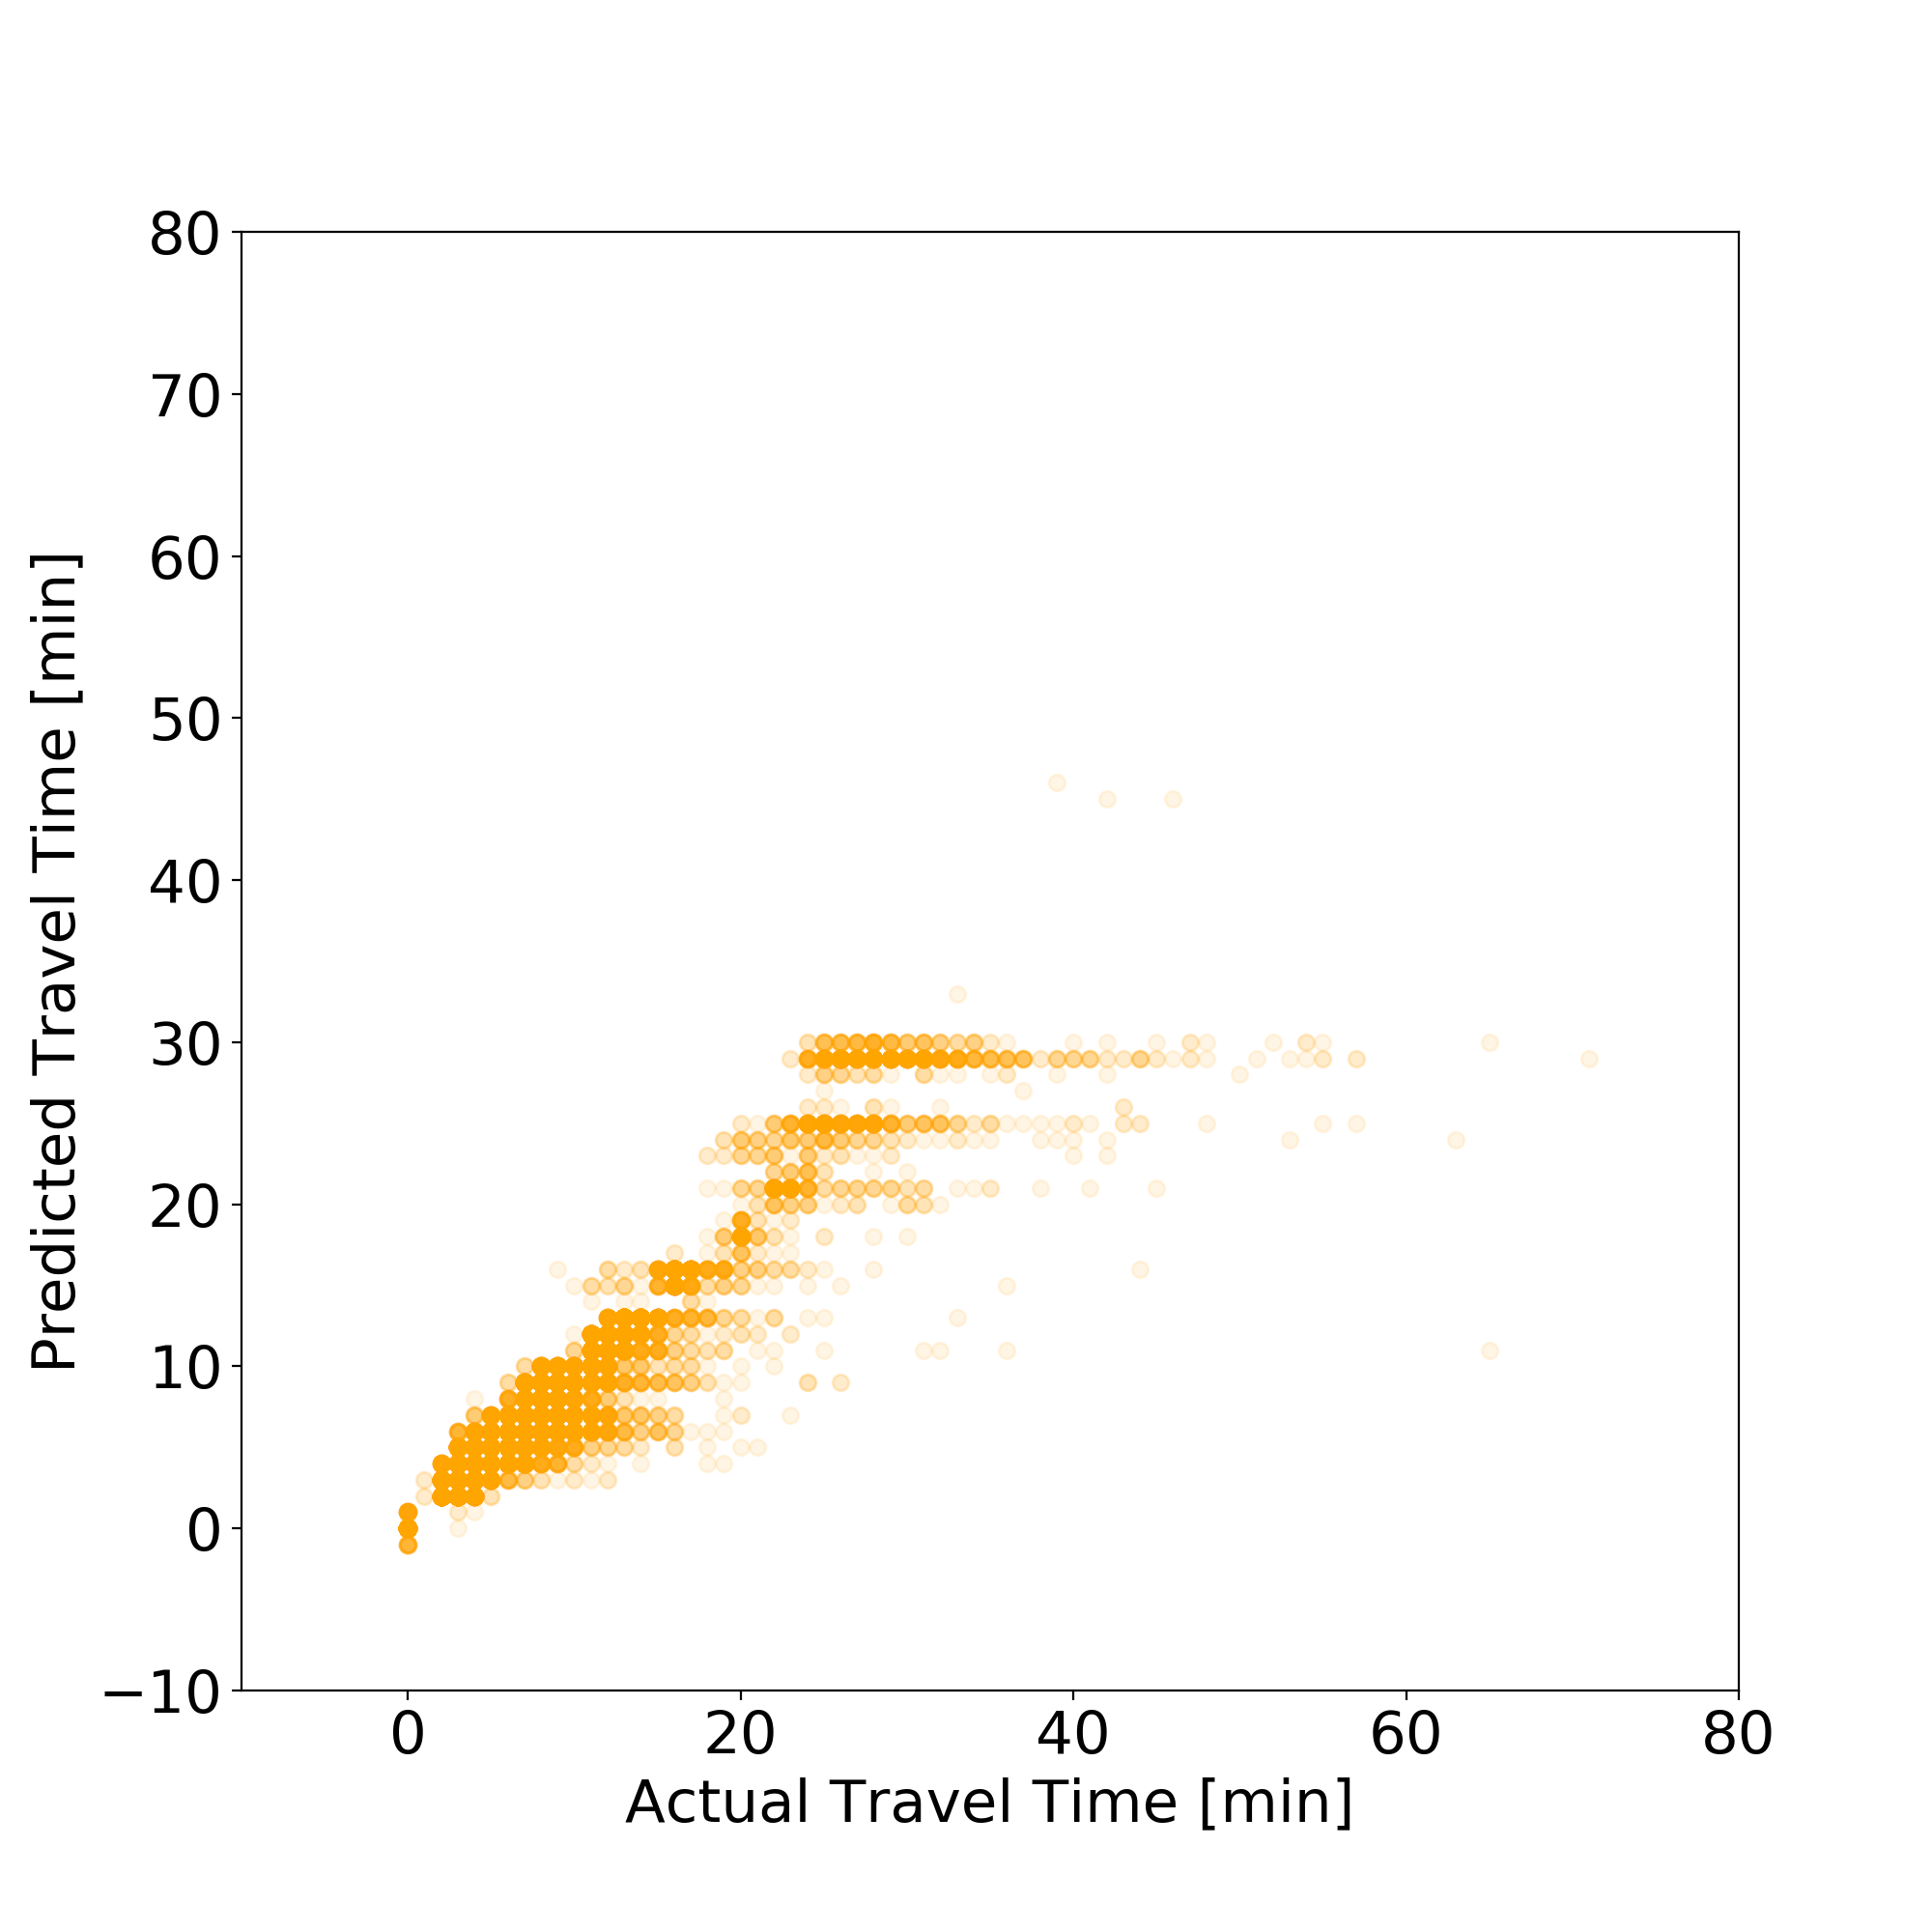
\includegraphics[width=0.5\textwidth]{Images/DNN_plot/7_step/7_step_travel_time.png}\label{fig:7_step_travel_time}}
\subfloat[\tiny{7-Step XGBoost Travel Time}]{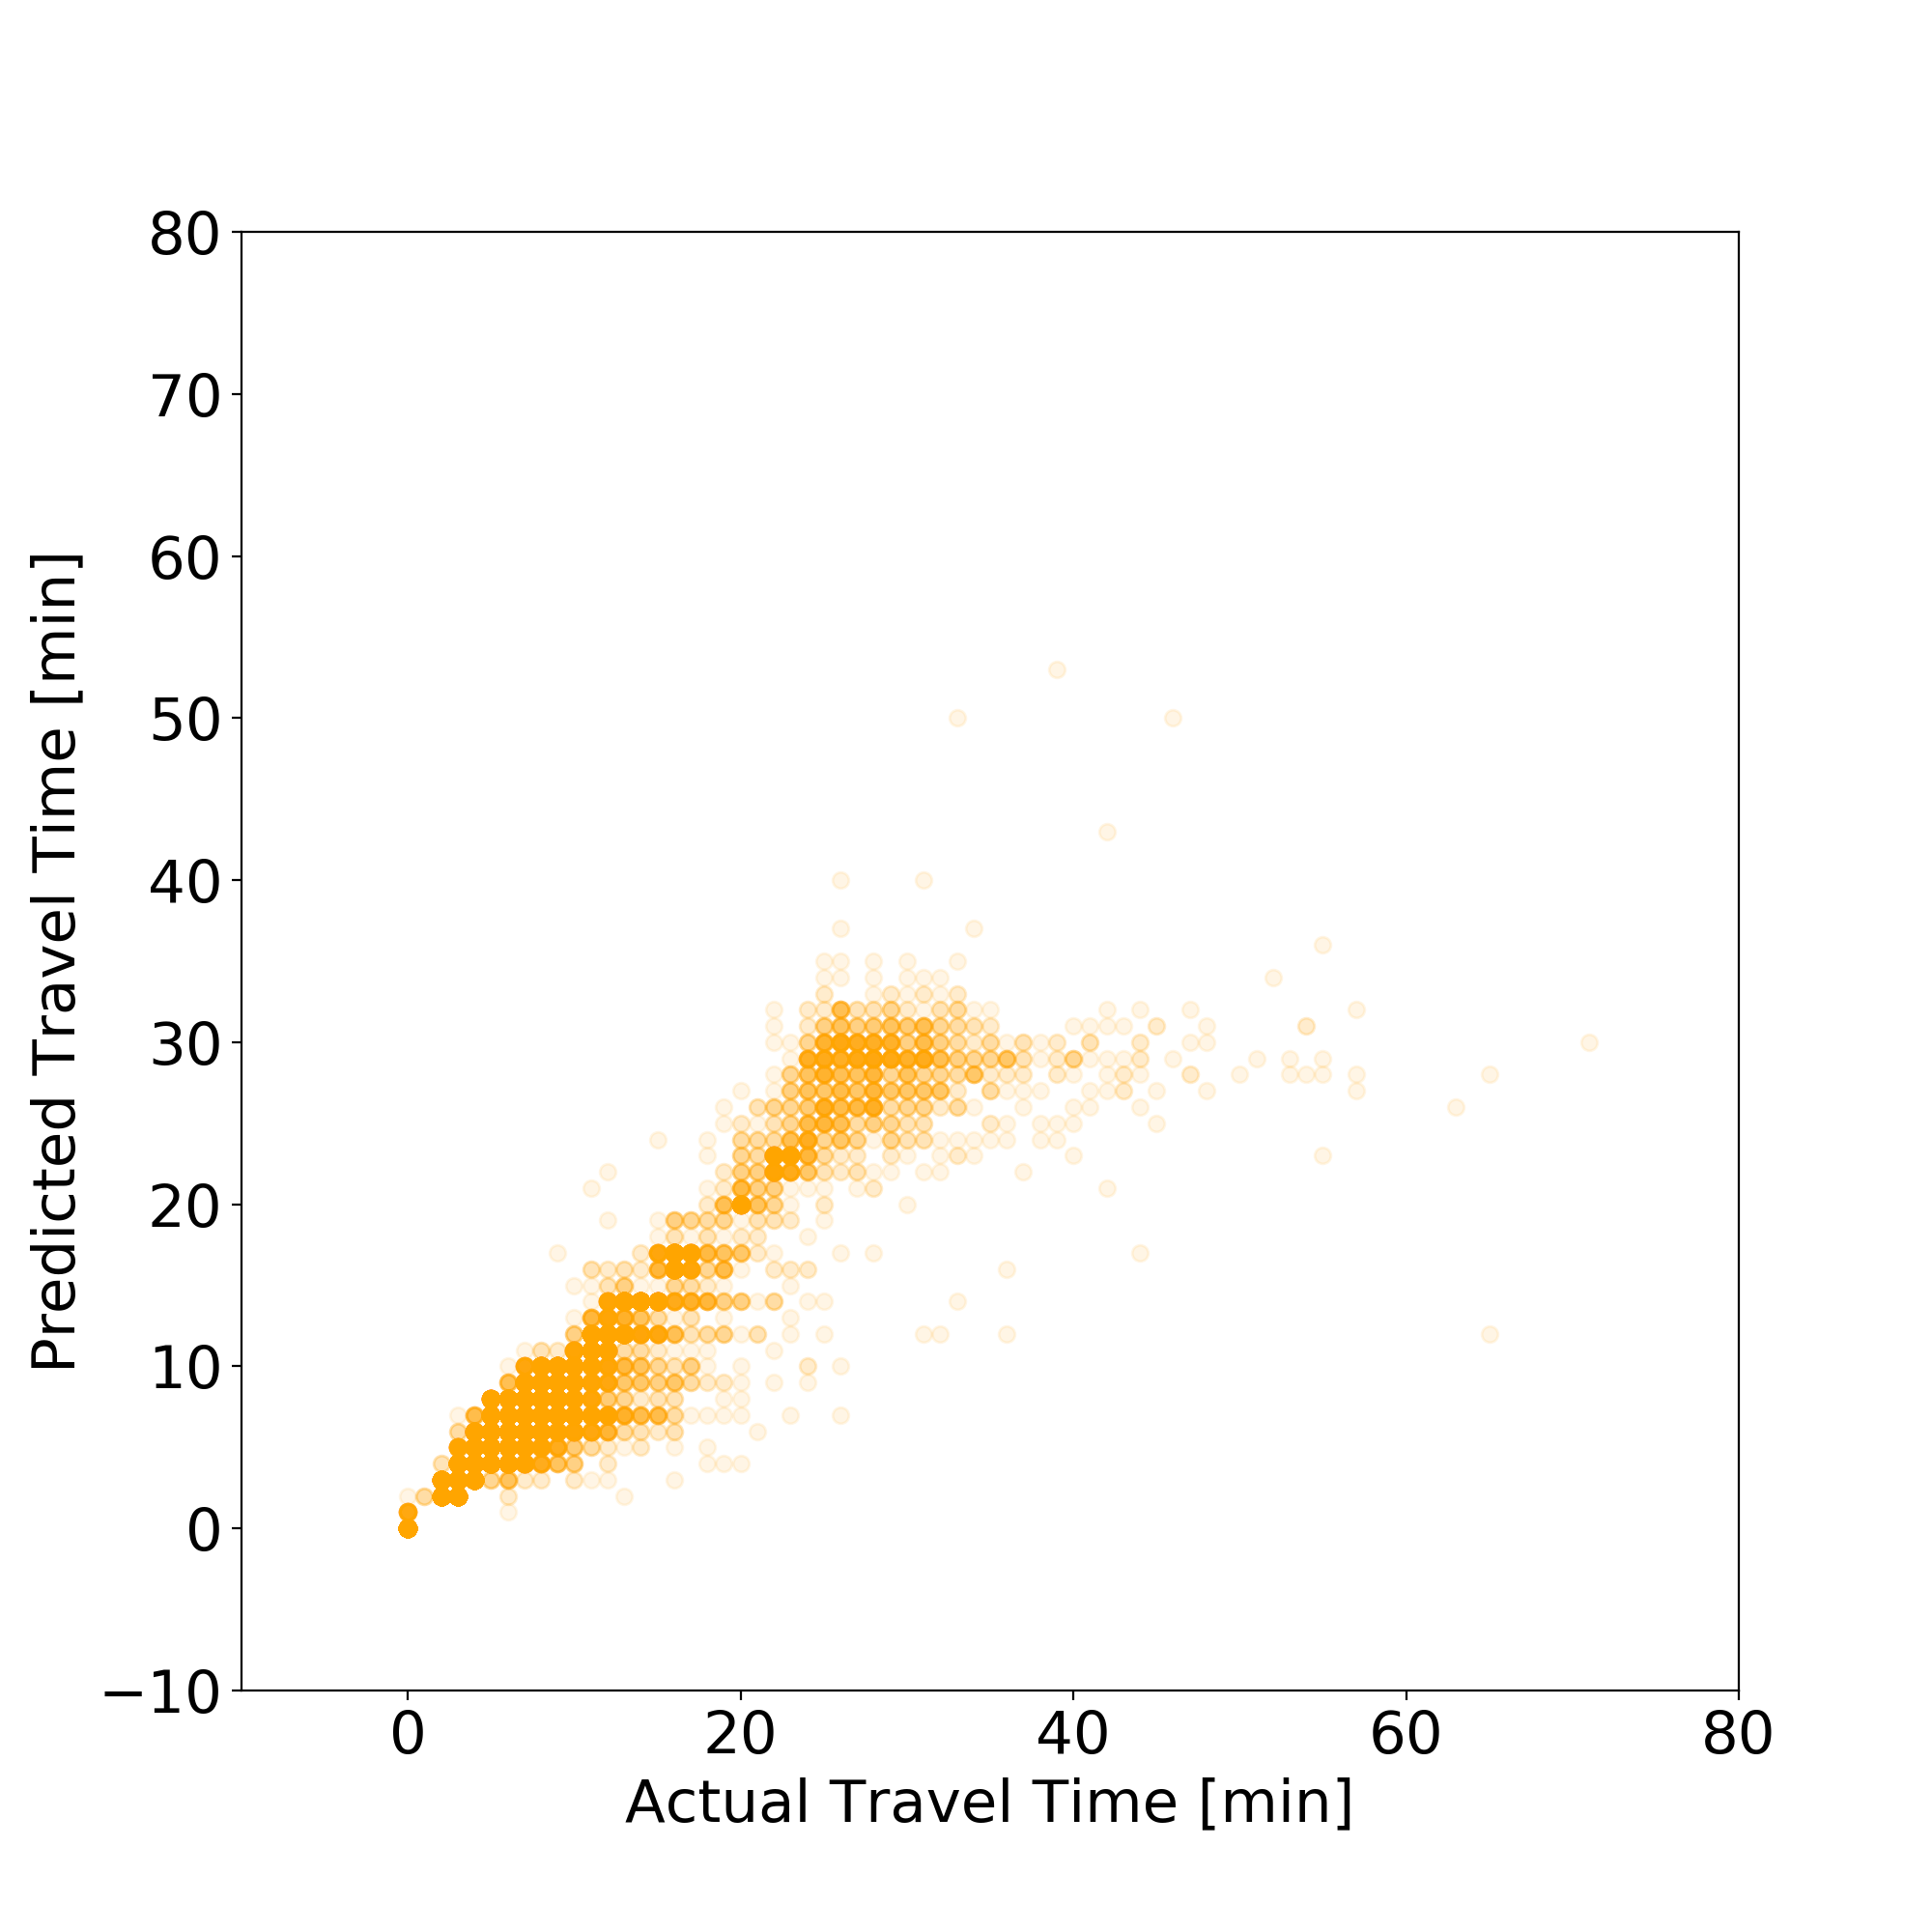
\includegraphics[width=0.5\textwidth]{Images/XGBoost_plot/7_step/7_step_travel_time.png}\label{fig:7_step_travel_time}}
\end{figure}
\begin{figure}[H]
\centering
\subfloat[\tiny{7-Step DNN Dwell Time}]{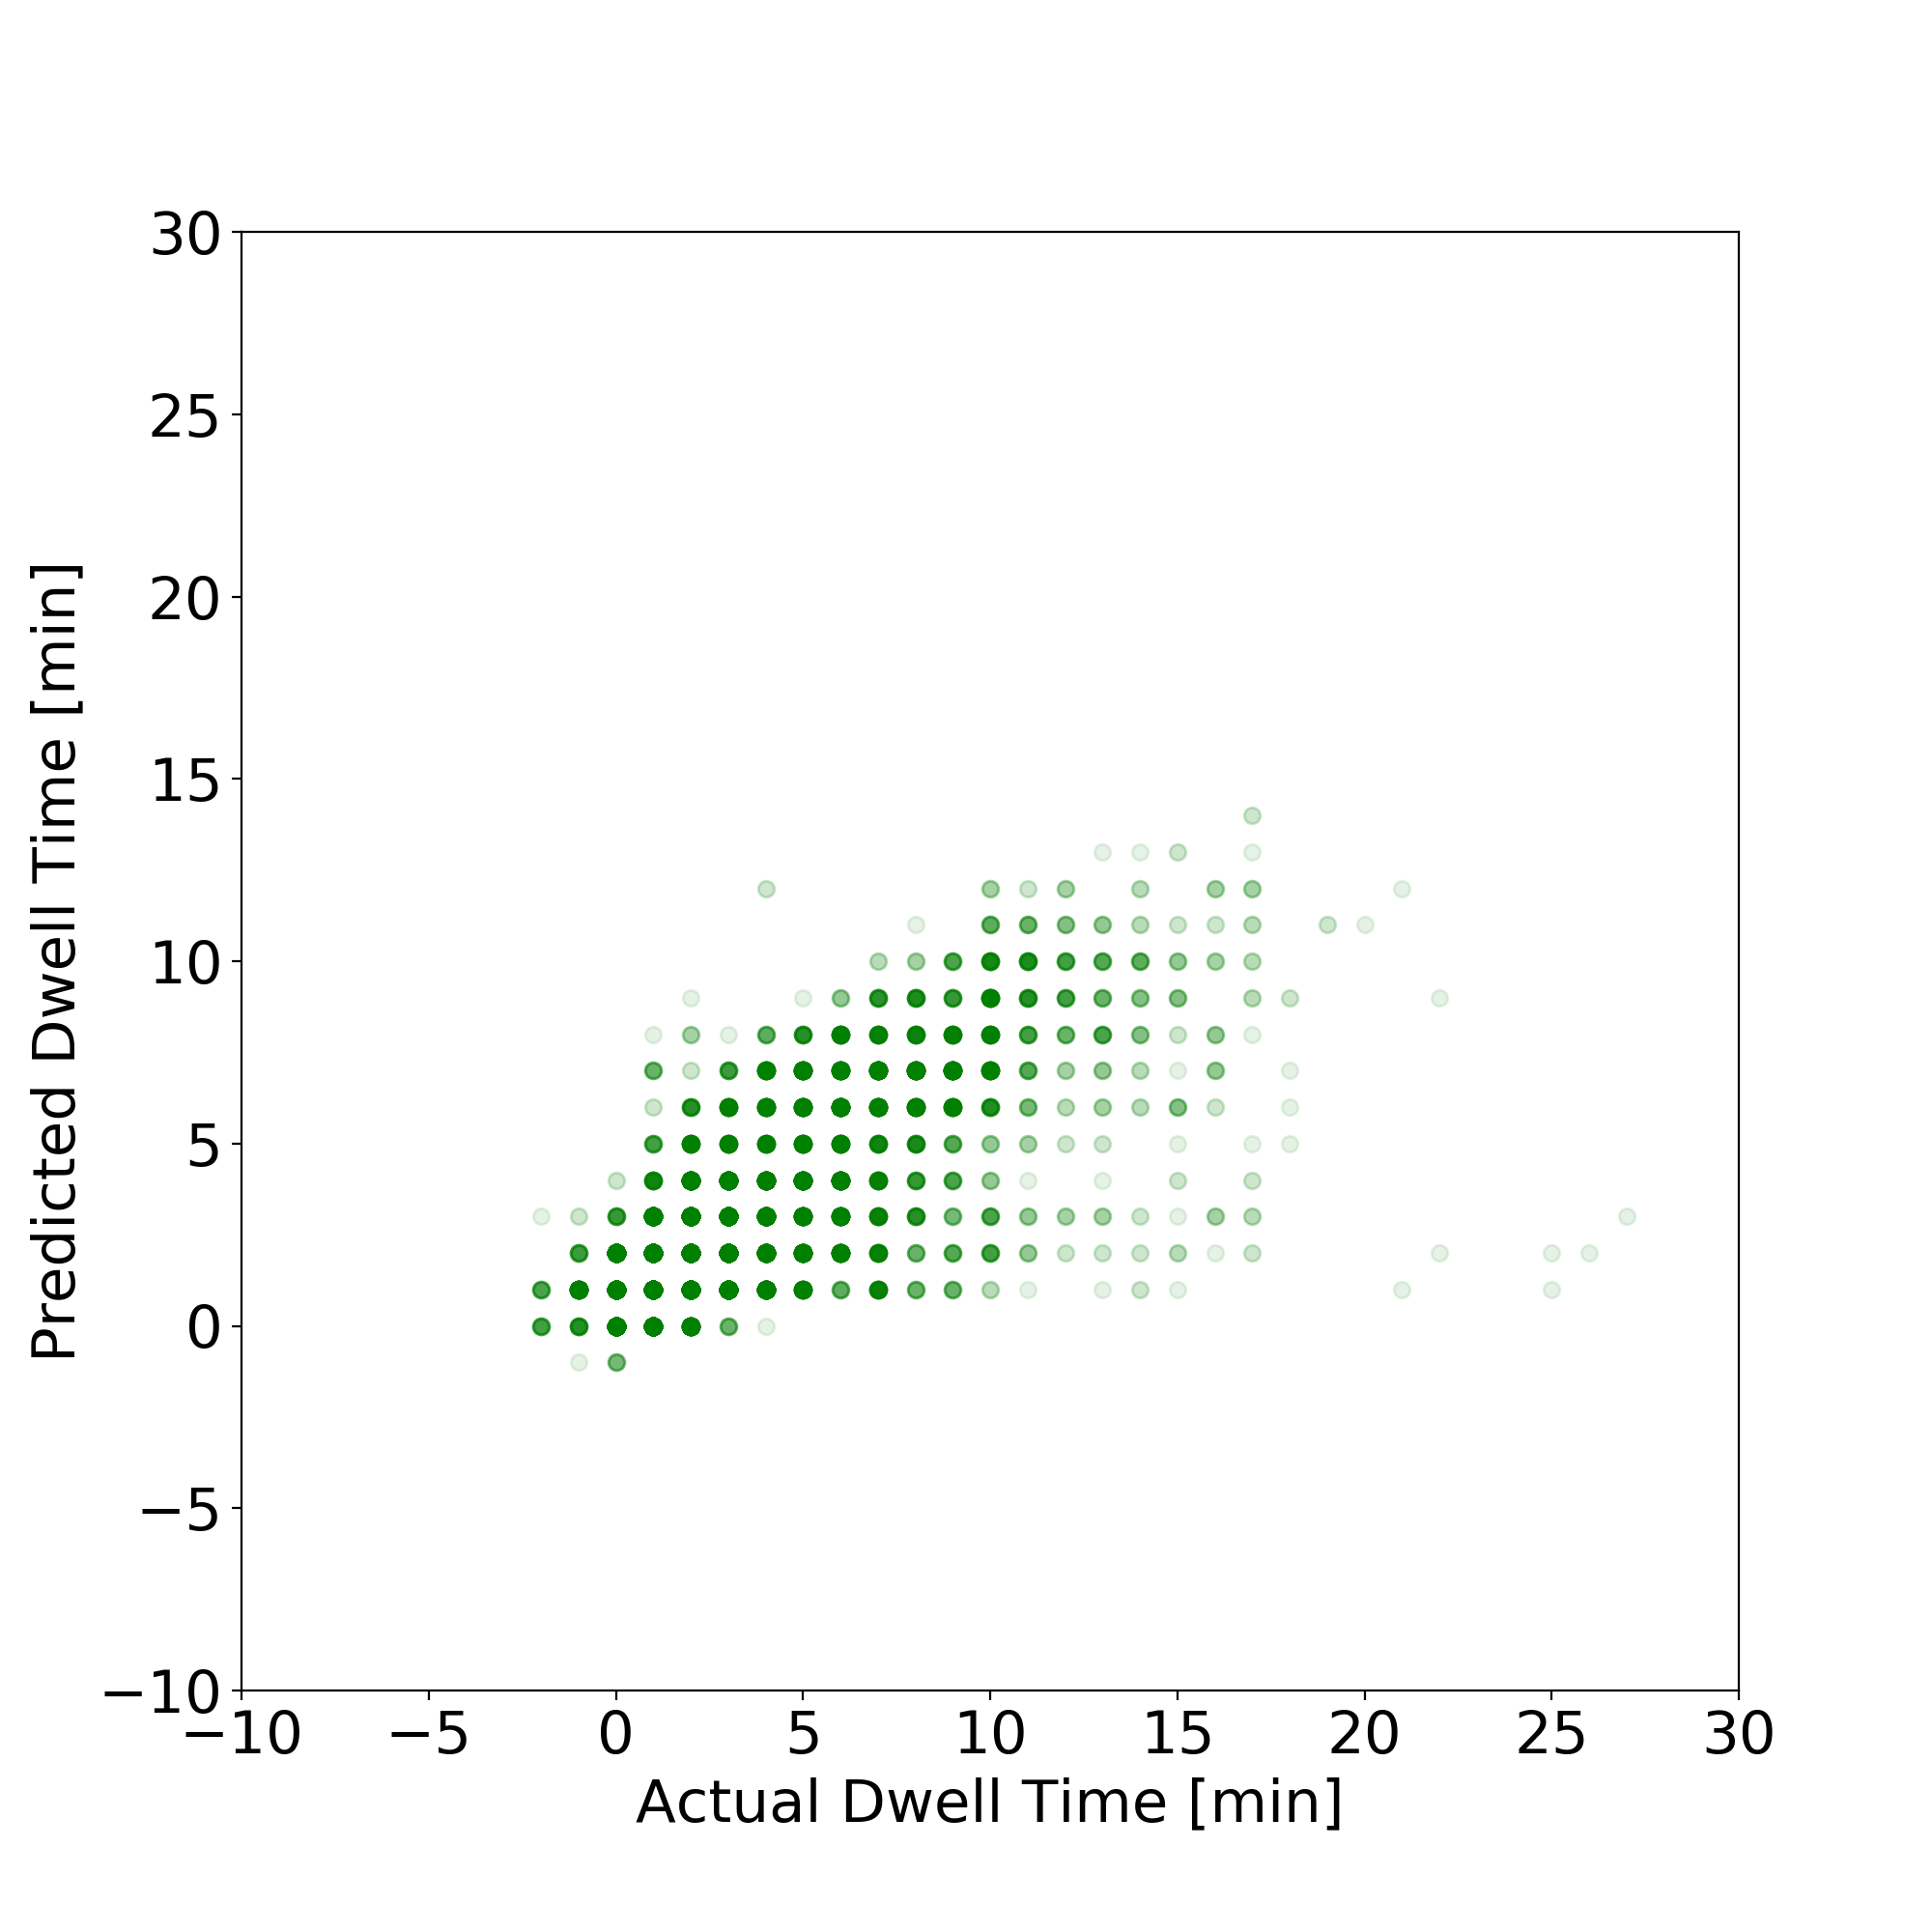
\includegraphics[width=0.5\textwidth]{Images/DNN_plot/7_step/7_step_dwell_time.png}\label{fig:7_step_dwell_time}}
\subfloat[\tiny{7-Step XGBoost Dwell Time}]{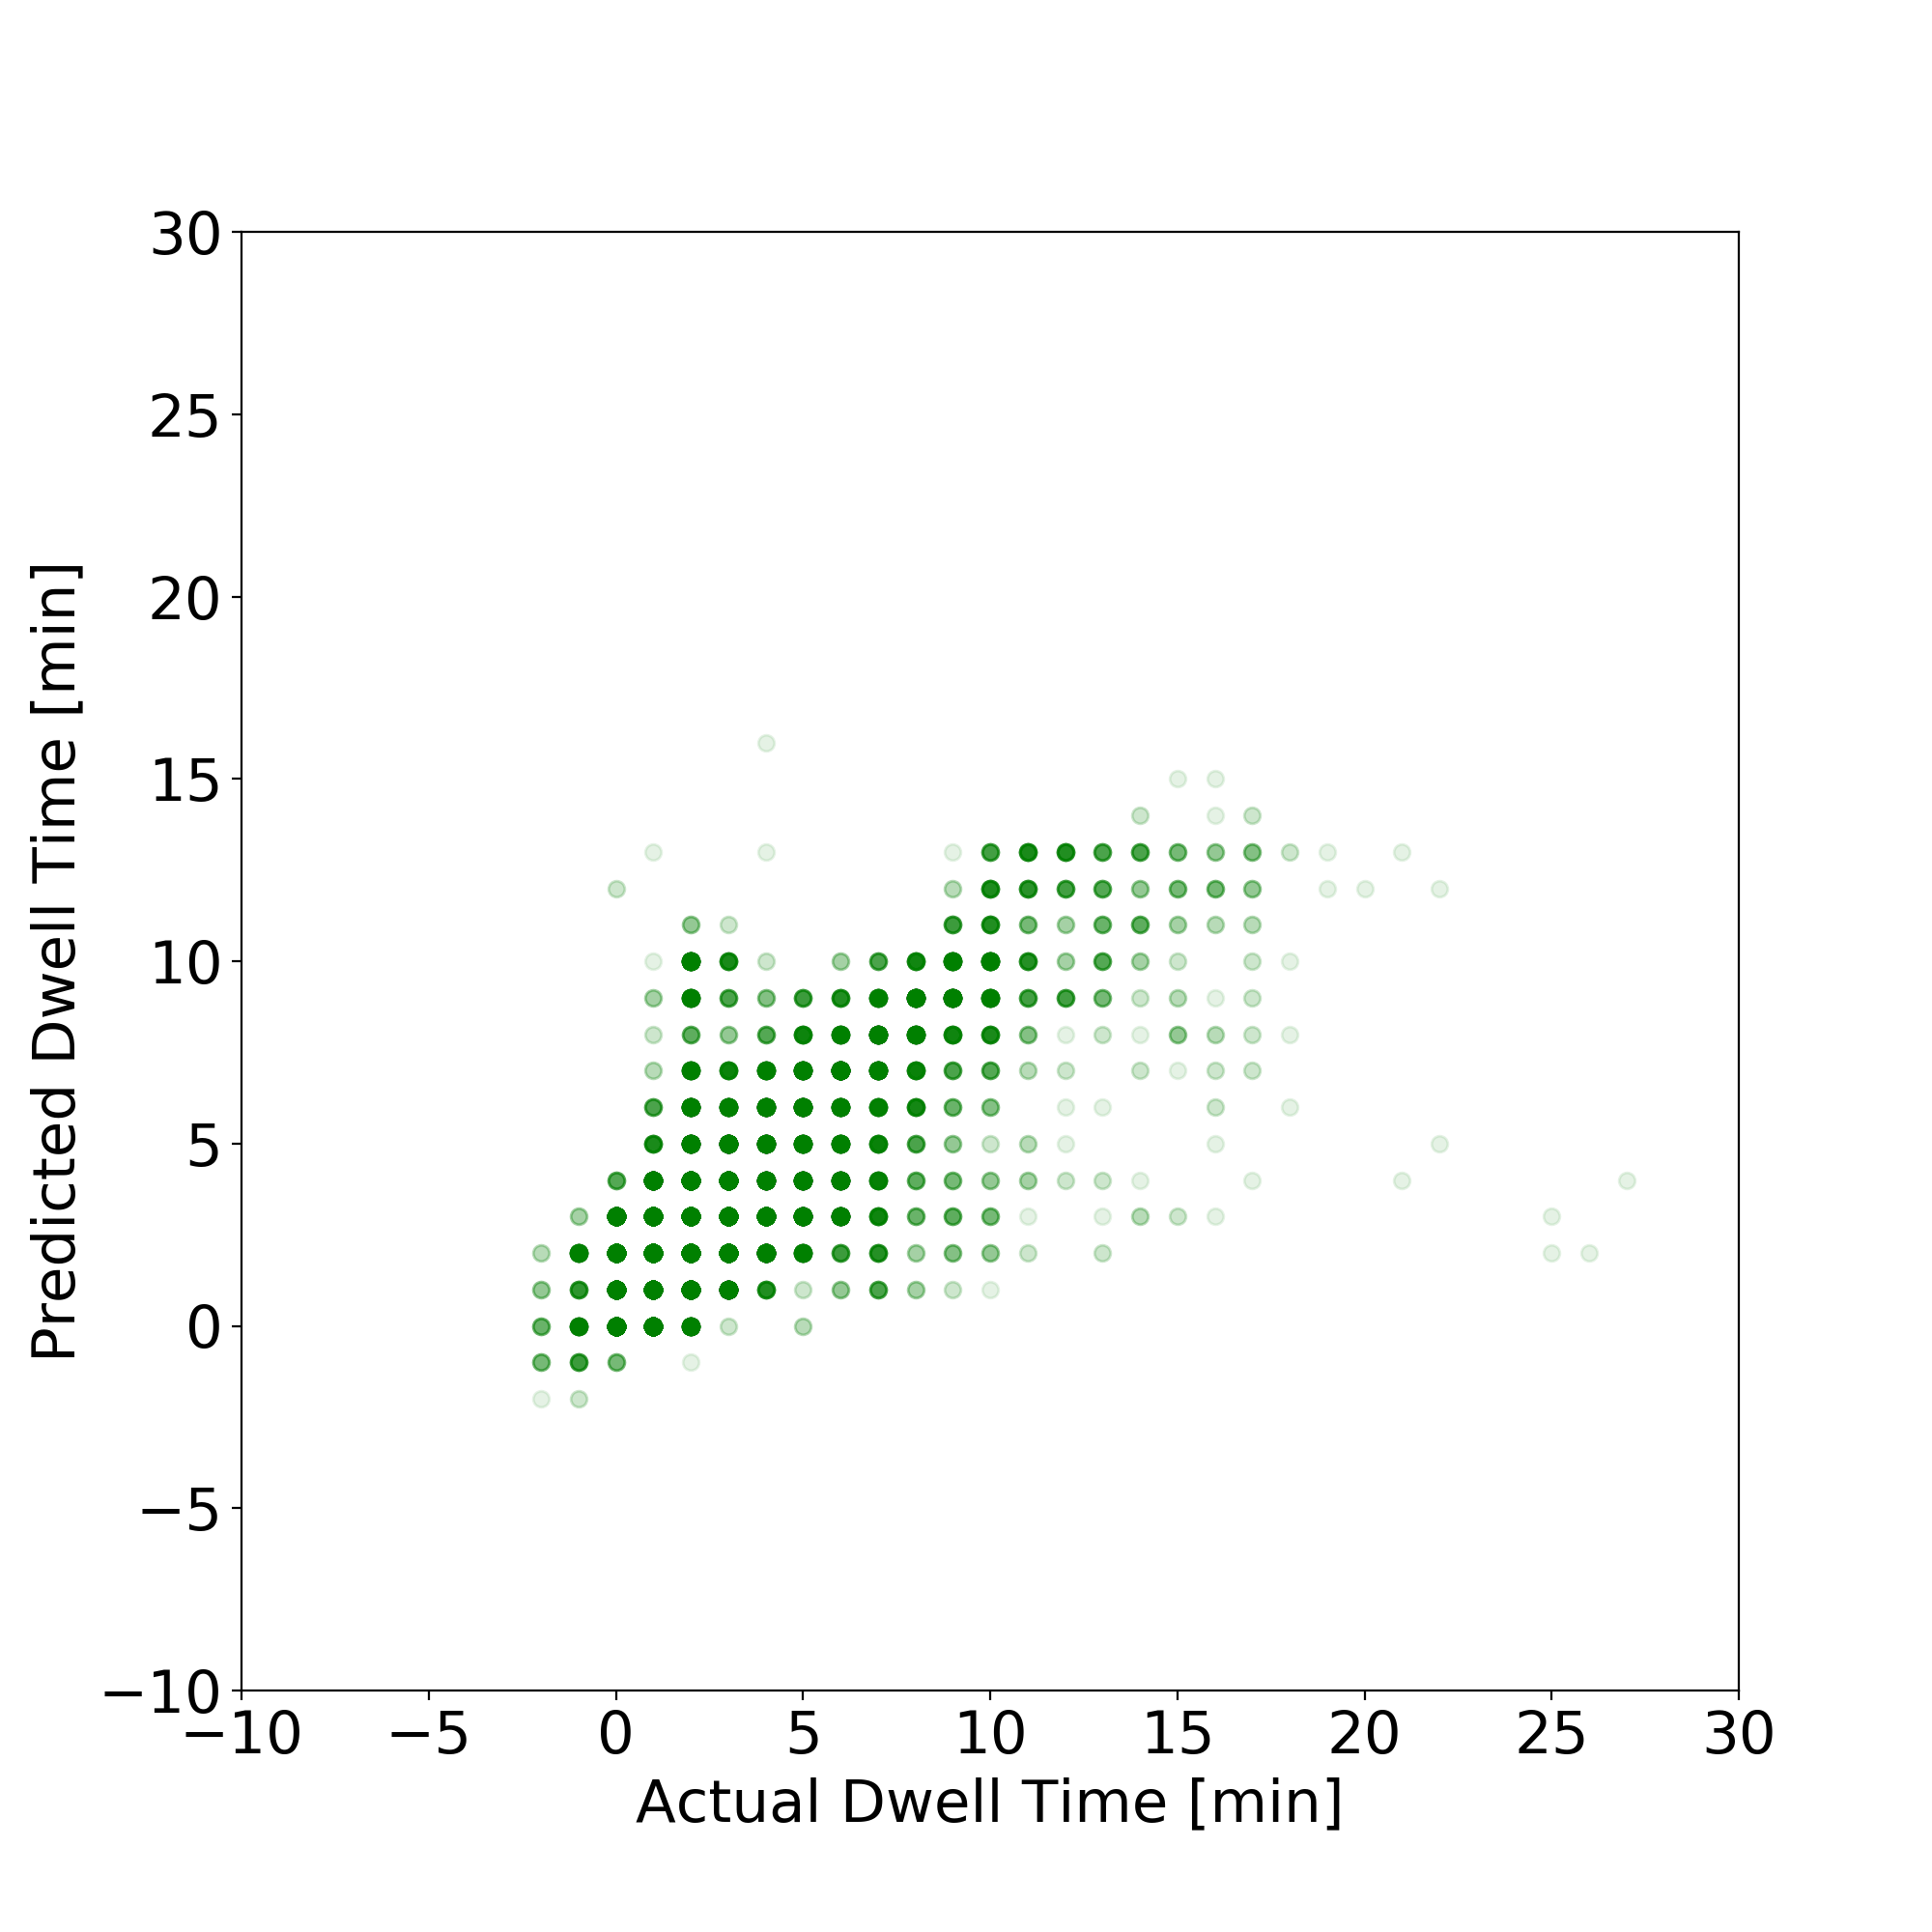
\includegraphics[width=0.5\textwidth]{Images/XGBoost_plot/7_step/7_step_dwell_time.png}\label{fig:7_step_dwell_time}}
\end{figure}

\begin{figure}[H]
\centering
\subfloat[\tiny{8-Step DNN Deviation from Arrival}]{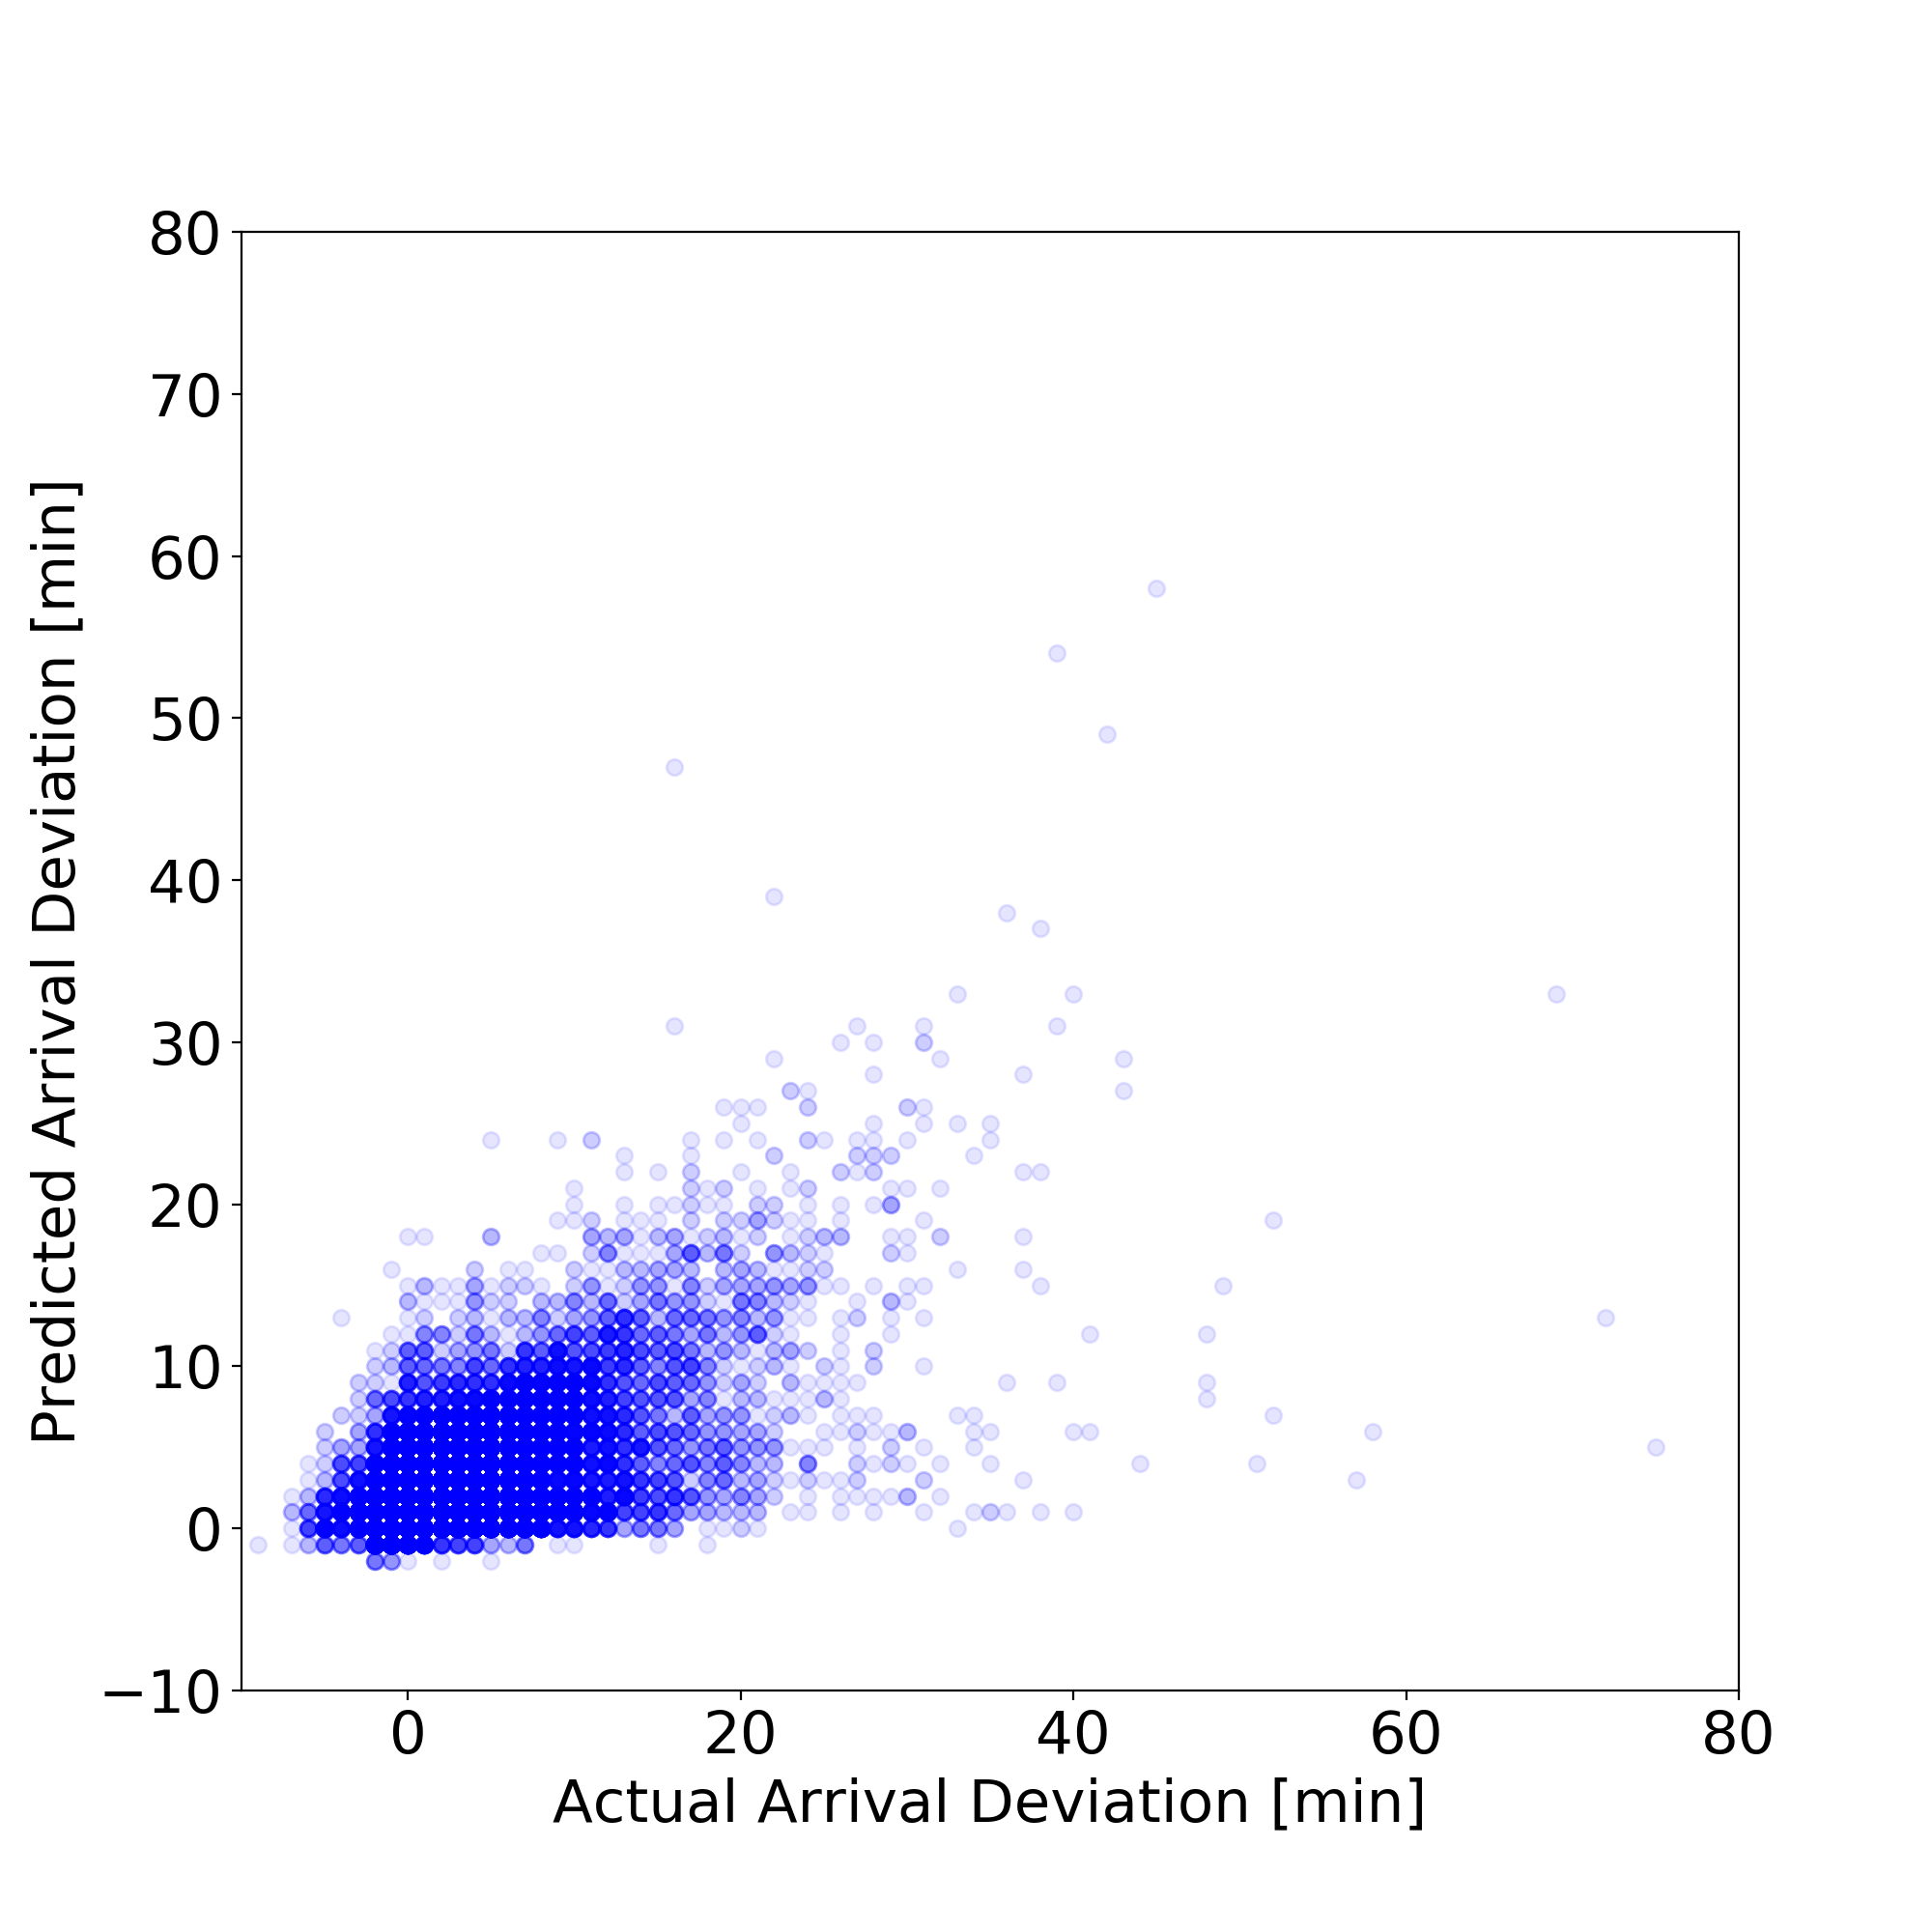
\includegraphics[width=0.5\textwidth]{Images/DNN_plot/8_step/8_step_arrival_deviation.png}\label{fig:8_step_arrival_deviation}}
\subfloat[\tiny{8-Step XGBoost Deviation from Arrival}]{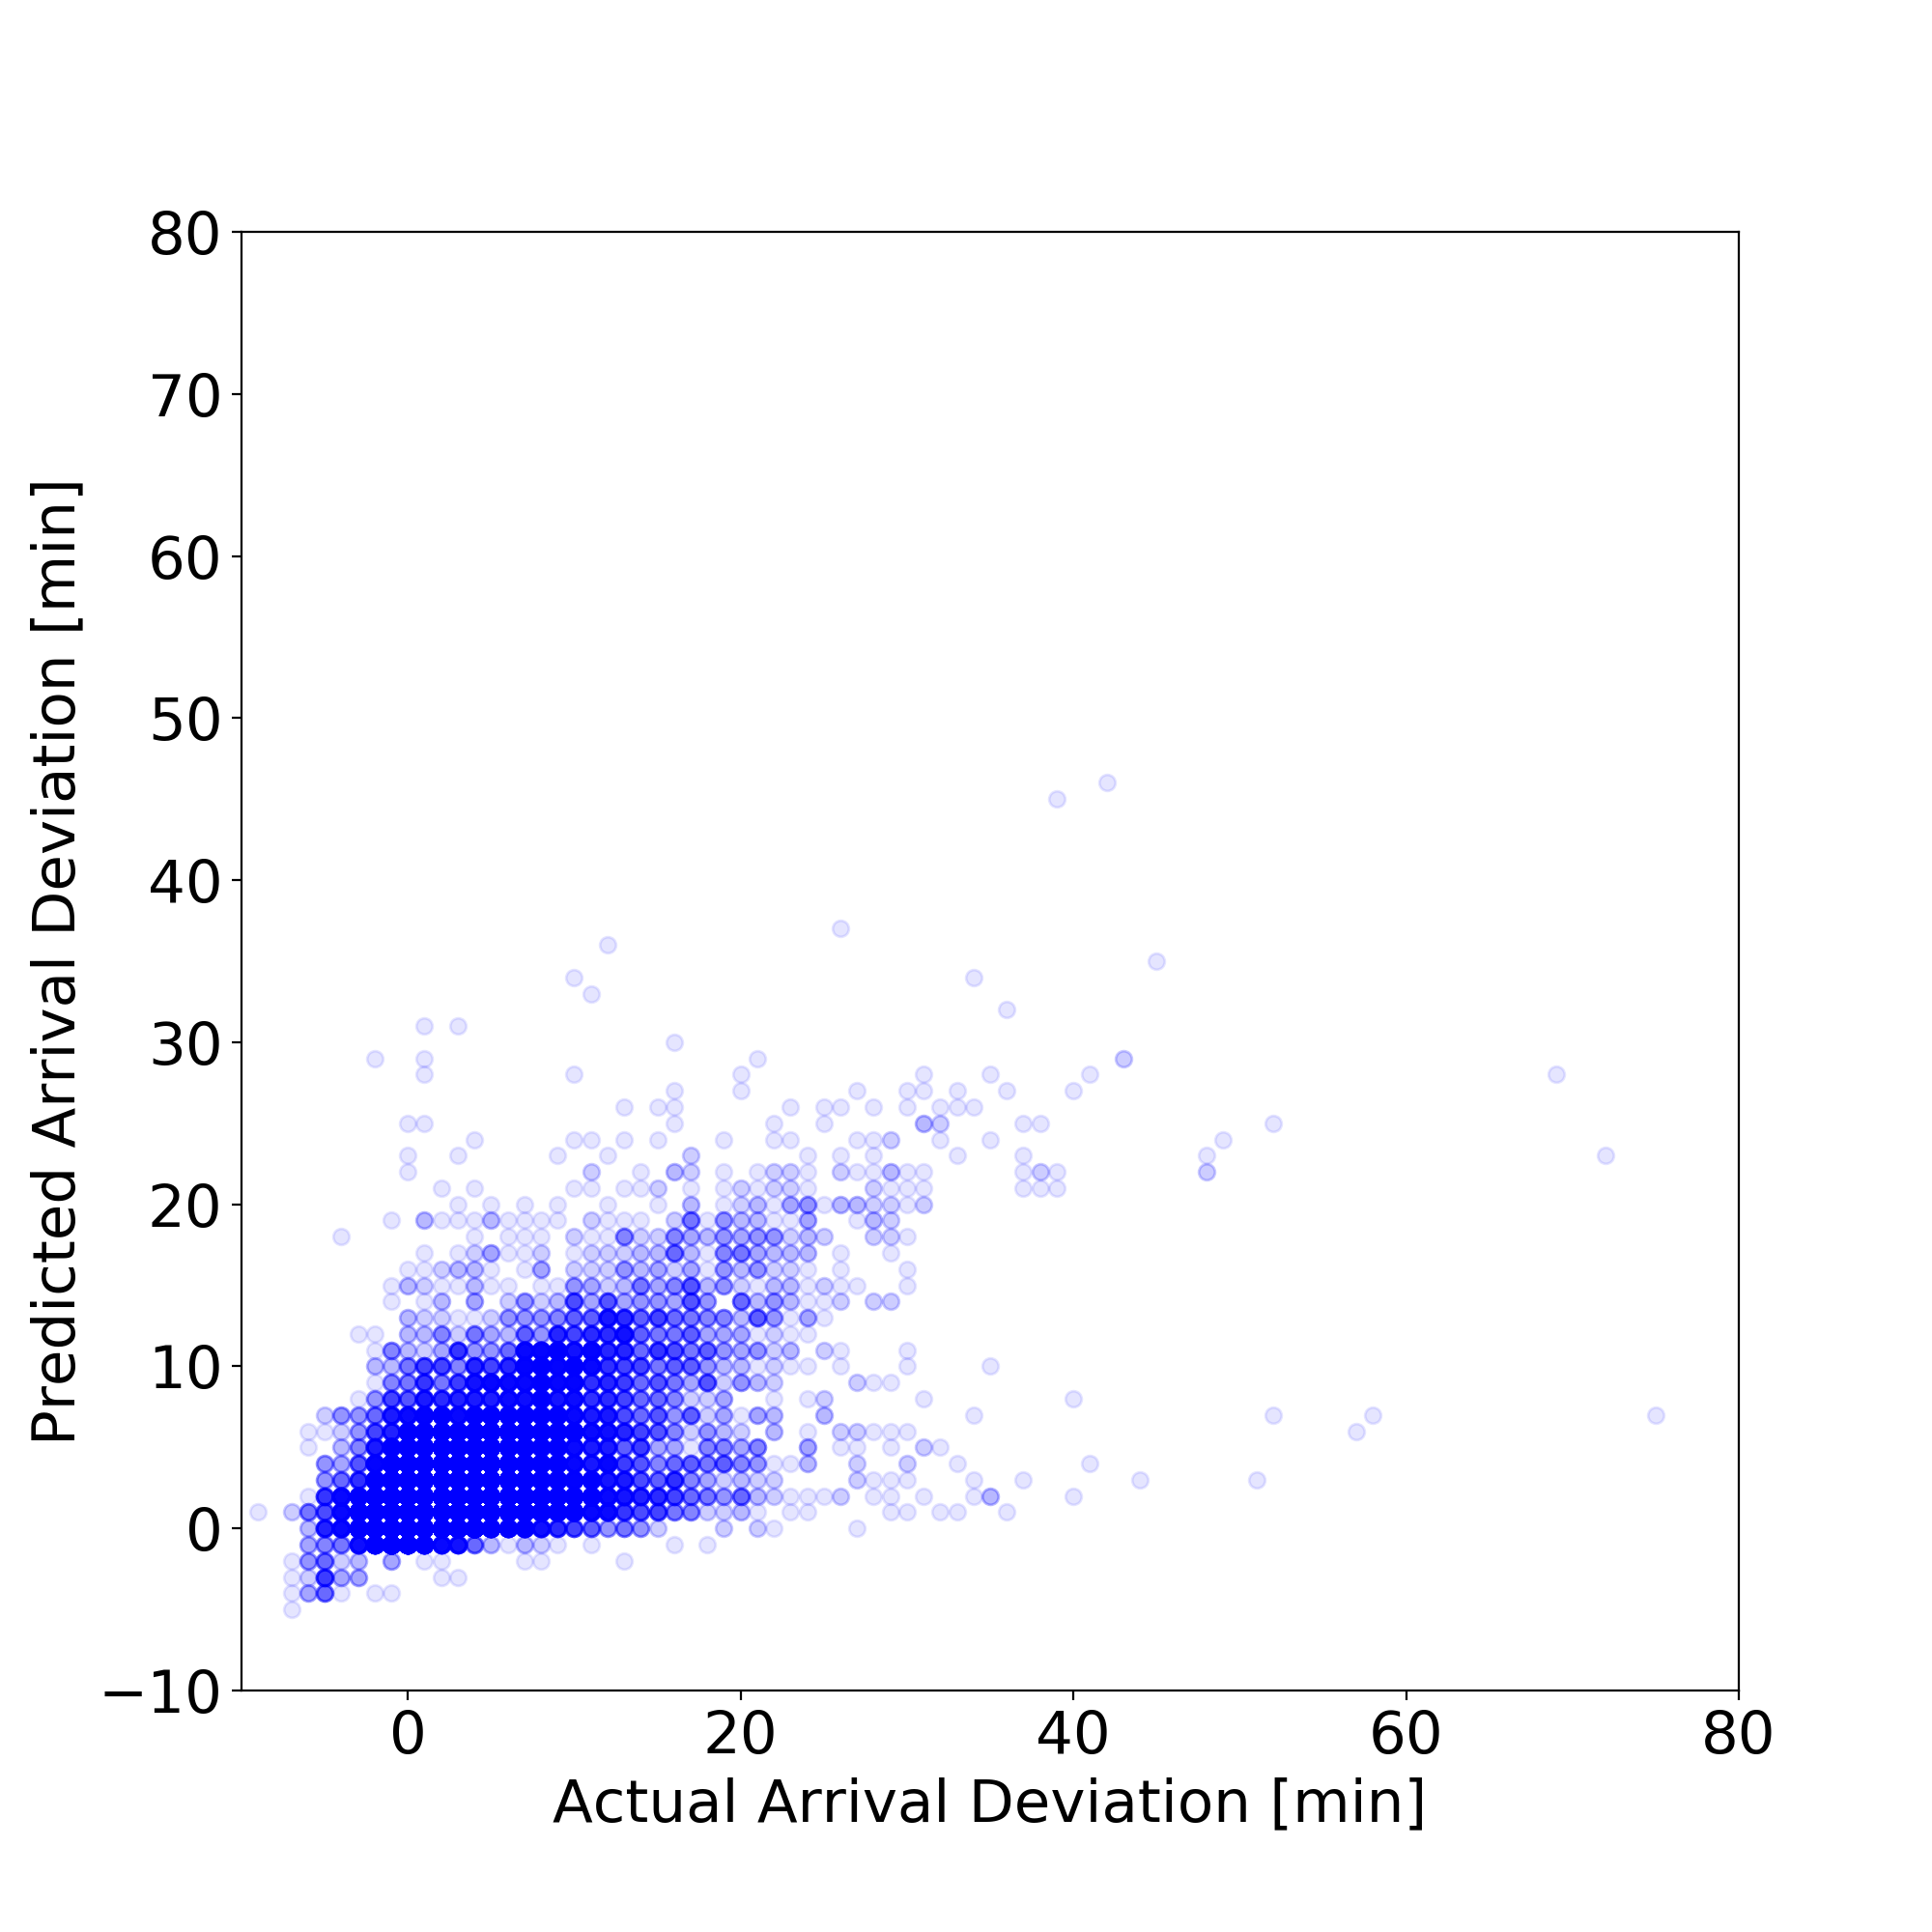
\includegraphics[width=0.5\textwidth]{Images/XGBoost_plot/8_step/8_step_arrival_deviation.png}\label{fig:8_step_arrival_deviation}}
\end{figure}
\begin{figure}[H]
\centering
\subfloat[\tiny{8-Step DNN Deviation from Departure}]{\includegraphics[width=0.5\textwidth]{Images/DNN_plot/8_step/8_step_depature_deviation.png}\label{fig:8_step_depature_deviation}}
\subfloat[\tiny{8-Step XGBoost Deviation from Departure}]{\includegraphics[width=0.5\textwidth]{Images/XGBoost_plot/8_step/8_step_depature_deviation.png}\label{fig:8_step_depature_deviation}}
\end{figure}
\begin{figure}[H]
\centering
\subfloat[\tiny{8-Step DNN Travel Time}]{\includegraphics[width=0.5\textwidth]{Images/DNN_plot/8_step/8_step_travel_time.png}\label{fig:8_step_travel_time}}
\subfloat[\tiny{8-Step XGBoost Travel Time}]{\includegraphics[width=0.5\textwidth]{Images/XGBoost_plot/8_step/8_step_travel_time.png}\label{fig:8_step_travel_time}}
\end{figure}
\begin{figure}[H]
\centering
\subfloat[\tiny{8-Step DNN Dwell Time}]{\includegraphics[width=0.5\textwidth]{Images/DNN_plot/8_step/8_step_dwell_time.png}\label{fig:8_step_dwell_time}}
\subfloat[\tiny{8-Step XGBoost Dwell Time}]{\includegraphics[width=0.5\textwidth]{Images/XGBoost_plot/8_step/8_step_dwell_time.png}\label{fig:8_step_dwell_time}}
\end{figure}

\begin{figure}[H]
\centering
\subfloat[\tiny{9-Step DNN Deviation from Arrival}]{\includegraphics[width=0.5\textwidth]{Images/DNN_plot/9_step/9_step_arrival_deviation.png}\label{fig:9_step_arrival_deviation}}
\subfloat[\tiny{9-Step XGBoost Deviation from Arrival}]{\includegraphics[width=0.5\textwidth]{Images/XGBoost_plot/9_step/9_step_arrival_deviation.png}\label{fig:9_step_arrival_deviation}}
\end{figure}
\begin{figure}[H]
\centering
\subfloat[\tiny{9-Step DNN Deviation from Departure}]{\includegraphics[width=0.5\textwidth]{Images/DNN_plot/9_step/9_step_depature_deviation.png}\label{fig:9_step_depature_deviation}}
\subfloat[\tiny{9-Step XGBoost Deviation from Departure}]{\includegraphics[width=0.5\textwidth]{Images/XGBoost_plot/9_step/9_step_depature_deviation.png}\label{fig:9_step_depature_deviation}}
\end{figure}
\begin{figure}[H]
\centering
\subfloat[\tiny{9-Step DNN Travel Time}]{\includegraphics[width=0.5\textwidth]{Images/DNN_plot/9_step/9_step_travel_time.png}\label{fig:9_step_travel_time}}
\subfloat[\tiny{9-Step XGBoost Travel Time}]{\includegraphics[width=0.5\textwidth]{Images/XGBoost_plot/9_step/9_step_travel_time.png}\label{fig:9_step_travel_time}}
\end{figure}
\begin{figure}[H]
\centering
\subfloat[\tiny{9-Step DNN Dwell Time}]{\includegraphics[width=0.5\textwidth]{Images/DNN_plot/9_step/9_step_dwell_time.png}\label{fig:9_step_dwell_time}}
\subfloat[\tiny{9-Step XGBoost Dwell Time}]{\includegraphics[width=0.5\textwidth]{Images/XGBoost_plot/9_step/9_step_dwell_time.png}\label{fig:9_step_dwell_time}}
\end{figure}

\begin{figure}[H]
\centering
\subfloat[\tiny{10-Step DNN Deviation from Arrival}]{\includegraphics[width=0.5\textwidth]{Images/DNN_plot/10_step/10_step_arrival_deviation.png}\label{fig:10_step_arrival_deviation}}
\subfloat[\tiny{10-Step XGBoost Deviation from Arrival}]{\includegraphics[width=0.5\textwidth]{Images/XGBoost_plot/10_step/10_step_arrival_deviation.png}\label{fig:10_step_arrival_deviation}}
\end{figure}
\begin{figure}[H]
\centering
\subfloat[\tiny{10-Step DNN Deviation from Departure}]{\includegraphics[width=0.5\textwidth]{Images/DNN_plot/10_step/10_step_depature_deviation.png}\label{fig:10_step_depature_deviation}}
\subfloat[\tiny{10-Step XGBoost Deviation from Departure}]{\includegraphics[width=0.5\textwidth]{Images/XGBoost_plot/10_step/10_step_depature_deviation.png}\label{fig:10_step_depature_deviation}}
\end{figure}
\begin{figure}[H]
\centering
\subfloat[\tiny{10-Step DNN Travel Time}]{\includegraphics[width=0.5\textwidth]{Images/DNN_plot/10_step/10_step_travel_time.png}\label{fig:10_step_travel_time}}
\subfloat[\tiny{10-Step XGBoost Travel Time}]{\includegraphics[width=0.5\textwidth]{Images/XGBoost_plot/10_step/10_step_travel_time.png}\label{fig:10_step_travel_time}}
\end{figure}
\begin{figure}[H]
\centering
\subfloat[\tiny{10-Step DNN Dwell Time}]{\includegraphics[width=0.5\textwidth]{Images/DNN_plot/10_step/10_step_dwell_time.png}\label{fig:10_step_dwell_time}}
\subfloat[\tiny{10-Step XGBoost Dwell Time}]{\includegraphics[width=0.5\textwidth]{Images/XGBoost_plot/10_step/10_step_dwell_time.png}\label{fig:10_step_dwell_time}}
\end{figure}

\section{DNN Training and Validation Loss}
\begin{figure}[H]
\centering
\subfloat[\tiny{1-Step}]{\includegraphics[width=75mm]{Images/DNN_validation/DNN_1_step_loss.png}}
\subfloat[\tiny{2-Step}]{\includegraphics[width=75mm]{Images/DNN_validation/DNN_2_step_loss.png}}
\end{figure}
\begin{figure}[H]
\subfloat[\tiny{3-Step}]{\includegraphics[width=75mm]{Images/DNN_validation/DNN_3_step_loss.png}}
\subfloat[\tiny{4-Step}]{\includegraphics[width=75mm]{Images/DNN_validation/DNN_4_step_loss.png}}
\end{figure}
\begin{figure}[H]
\subfloat[\tiny{5-Step}]{\includegraphics[width=75mm]{Images/DNN_validation/DNN_5_step_loss.png}}
\subfloat[\tiny{6-Step}]{\includegraphics[width=75mm]{Images/DNN_validation/DNN_6_step_loss.png}}
\end{figure}
\begin{figure}[H]
\subfloat[\tiny{7-Step}]{\includegraphics[width=75mm]{Images/DNN_validation/DNN_7_step_loss.png}}
\subfloat[\tiny{8-Step}]{\includegraphics[width=75mm]{Images/DNN_validation/DNN_8_step_loss.png}}
\end{figure}
\begin{figure}[H]
\subfloat[\tiny{9-Step}]{\includegraphics[width=75mm]{Images/DNN_validation/DNN_9_step_loss.png}}
\subfloat[\tiny{10-Step}]{\includegraphics[width=75mm]{Images/DNN_validation/DNN_10_step_loss.png}}
\end{figure}

\section{XGBoost Training and Validation Loss}
\begin{figure}[H]
\centering
\subfloat[\tiny{1-Step}]{\includegraphics[width=75mm]{Images/XGBoost_validation/XGBoost_1_step_loss.png}}
\subfloat[\tiny{2-Step}]{\includegraphics[width=75mm]{Images/XGBoost_validation/XGBoost_2_step_loss.png}}
\end{figure}
\begin{figure}[H]
\subfloat[\tiny{3-Step}]{\includegraphics[width=75mm]{Images/XGBoost_validation/XGBoost_3_step_loss.png}}
\subfloat[\tiny{4-Step}]{\includegraphics[width=75mm]{Images/XGBoost_validation/XGBoost_4_step_loss.png}}
\end{figure}
\begin{figure}[H]
\subfloat[\tiny{5-Step}]{\includegraphics[width=75mm]{Images/XGBoost_validation/XGBoost_5_step_loss.png}}
\subfloat[\tiny{6-Step}]{\includegraphics[width=75mm]{Images/XGBoost_validation/XGBoost_6_step_loss.png}}
\end{figure}
\begin{figure}[H]
\subfloat[\tiny{7-Step}]{\includegraphics[width=75mm]{Images/XGBoost_validation/XGBoost_7_step_loss.png}}
\subfloat[\tiny{8-Step}]{\includegraphics[width=75mm]{Images/XGBoost_validation/XGBoost_8_step_loss.png}}
\end{figure}
\begin{figure}[H]
\subfloat[\tiny{9-Step}]{\includegraphics[width=75mm]{Images/XGBoost_validation/XGBoost_9_step_loss.png}}
\subfloat[\tiny{10-Step}]{\includegraphics[width=75mm]{Images/XGBoost_validation/XGBoost_10_step_loss.png}}
\end{figure}


\end{document}
